%%%%%%%%%%%%%%%%%%%%%%%%%%%%%%%%%%%%%%%%%%%%%%%%%%%%%%%%%%%%%%%%%%%%%%%%%%%%%%%%
% Preámbulo                                                                    %
%%%%%%%%%%%%%%%%%%%%%%%%%%%%%%%%%%%%%%%%%%%%%%%%%%%%%%%%%%%%%%%%%%%%%%%%%%%%%%%%

\documentclass[11pt,a4paper,titlepage,oneside]{report}

%%% RELACIÓN DE VARIABLES A PERSONALIZAR %%%
%\def\lingua{gal}
\def\lingua{esp} % descomenta esta liña se redactarás a memoria en español
%\def\lingua{eng} % descomenta esta liña se redactarás a memoria en inglés
\def\nome{Catarina García Cal}                             % substitúe aquí o teu nome
\def\nomedirectorA{Emilio José Padrón González}              % substitúe aquí o nome de quen dirixe
%\def\nomedirectorB{Outro Nome Completo}             % duplica esta liña máis veces se o precisas, cambiando
                                                     % a letra final (A, B, C, D...): úsanse na portada.tex
\def\titulo{Software de gestión de contratación con arquitectura Java EE multicapa para empresas proveedoras de servicios} % substitúe aquí o título do teu TFG
%\def\mencion{NOME DA MENCIÓN}                        % descomenta a mención correspondente
%\def\mencion{COMPUTACIÓN}
%\def\mencion{ENXEÑARÍA DO SOFTWARE}
%\def\mencion{ENXEÑARÍA DE COMPUTADORES}
%\def\mencion{SISTEMAS DE INFORMACIÓN}
\def\mencion{TECNOLOXÍAS DA INFORMACIÓN}

\def\renomearcadros{si} % descomenta esta liña se redactas a memoria en español e prefires que
                         % os "cuadros" e o "índice de cuadros" se renomeen
                         % a "tablas" e "índice de tablas" respectivamente

\usepackage{estilo_tfg}
\usepackage{csquotes}

% Lista de paquetes potencialmente interesantes (uso baixo demanda)

% \usepackage{alltt}       % proporciona o entorno alltt, semellante a verbatim pero que respecta comandos
% \usepackage{enumitem}    % permite personalizar os entornos de lista
% \usepackage{eurofont}    % proporciona o comando \euro
% \usepackage{float}       % permite máis opcións para controlar obxectos flotantes (táboas, figuras)
% \usepackage{hhline}      % permite personalizar as liñas horizontais en arrays e táboas
\usepackage{longtable}   % permite construir táboas que ocupan máis dunha páxina
\usepackage{lscape}      % permite colocar partes do documento en orientación apaisada
% \usepackage{moreverb}    % permite personalizar o entorno verbatim
% \usepackage{multirow}    % permite crear celdas que ocupan varias filas da mesma táboa
% \usepackage{pdfpages}    % permite insertar ficheiros en PDF no documento
% \usepackage{rotating}    % permite diferentes tipos de rotacións para figuras e táboas
% \usepackage{subcaption}  % permite a inclusión de varias subfiguras nunha figura
% \usepackage{tabu}        % permite táboas flexibles
% \usepackage{tabularx}    % permite táboas con columnas de anchura determinada

\usepackage{amsmath}
\usepackage{amsfonts}
\usepackage{amssymb}
\usepackage{geometry} % para poder usar vi\'netas en la tabla (\begin{table})
\usepackage{array} % para poder usar vi\'netas en la tabla (\begin{table})
\usepackage{graphicx} % para fijar la tabla en la posici\'on en la que se encuentra [H]
\usepackage{float}  % para fijar la tabla en la posici\'on en la que se encuentra [H]
\usepackage[normalem]{ulem} % para disponer de subrayado multilínea

\usepackage[acronym]{glossaries}
\usepackage[toc]{glossaries}

\lstdefinestyle{comando}{language=Bash,numbers=none,frame=none,
  escapeinside={(*}{*)},commentstyle=\itshape\color{black!60}}

\usepackage{hyperref}  

%%%%%%%%%%%%%%%%%%%%%%%%%%%%%%%%%%%%%%%%%%%%%%%%%%%%%%%%%%%%%%%%%%%%%%%%%%%%%%%%
% Corpo                                                                        %
%%%%%%%%%%%%%%%%%%%%%%%%%%%%%%%%%%%%%%%%%%%%%%%%%%%%%%%%%%%%%%%%%%%%%%%%%%%%%%%%

\begin{document}

 %%%%%%%%%%%%%%%%%%%%%%%%%%%%%%%%%%%%%%%%
 % Preliminares do documento            %
 %%%%%%%%%%%%%%%%%%%%%%%%%%%%%%%%%%%%%%%%

 \begin{titlepage}
  
  \hspace*{128pt}
  \textcolor{udcpink}{{\fontencoding{T1}\fontfamily{phv}\selectfont Facultade de Informática}}\\[-32pt]

  \begin{center}
    
\includegraphics[scale=0.3]{imaxes/udc}\\[25pt]

    {\large TRABALLO FIN DE GRAO \\
            GRAO EN ENXEÑARÍA INFORMÁTICA \\
            MENCIÓN EN \mencion } \\[10pt]

    
\includegraphics[scale=0.08]{imaxes/euro_inf_seal_bachelor_light background}\\[25pt]

    \begin{huge}
      \begin{spacing}{1.3}
        \bfseries \titulo
      \end{spacing}
    \end{huge}
  \end{center}
  
  \vfill
  
  \begin{flushright}
    {\large
    \begin{tabular}{ll}
      {\bf Estudante:} & \nome \\
      {\bf Dirección:} & \nomedirectorA \\
%                      & \nomedirectorB \\ % duplica esta liña máis veces se o precisas, cambiando
                                           % a letra final (A, B, C, D...); define eses nomes no memoria_tfg.tex
    \end{tabular}}
  \end{flushright}
  \rightline{A Coruña, \datasimple.}
\end{titlepage}

 \dedicatoria{A mis padres.} % escribe neste comando o teu texto de dedicatoria
 
 \paxinaenbranco
 \begin{agradecementos}
 Mi gratitud incondicional a todas y cada una de las personas que han colaborado en la realización de este trabajo.\\ 
 A mi tutor de proyecto, Emilio José Padrón González por aceptar mi propuesta de TFG y conseguir que la llevara a cabo con su continua comprensión, apoyo y motivación para finalizar este trabajo.\\
 A mis amigos que siempre tuvieron palabras de ánimo en los momentos en los que compaginar trabajo y estudios se tornaba un imposible. \\
 A mi familia, por su apoyo y confianza incondicional en todo lo que emprendo. \\
 A todos, gracias.
 \end{agradecementos}
 %%%%%%%%%%%%%%%%%%%%%%%%%%%%%%%%%%%%%%%%%%%%%%%%%%%%%%%%%%%%%%%%%%%%%%%%%%%%%%%%

\pagestyle{empty}
\begin{abstract}
	El presente trabajo presenta una aplicación de gestión de contratación basada en \gls{opensource} con arquitectura \acrlong{jee} multicapa, que pueda ser usada por cualquier proveedor de servicios con una cartera de clientes y un catálogo de productos y servicios facturables. Dichos clientes podrán contratar los diferentes productos y servicios del catálogo, a los que se les podrá aplicar descuentos sobre los correspondiente elementos facturables asociados, registrándose dicha relación contractual en la aplicación.
Además de la implementación de las distintas contrataciones la aplicación permitirá definir el catálogo de productos y servicios junto con las parametrizaciones pertinentes, como pueden ser los tipos de tasas aplicables sobre las distintas entidades facturables, o los ciclos de facturación asociados a los clientes.\\

  \vspace*{25pt}
  \begin{segundoresumo}
   This paper presents an open-source-based contract management application with multilayer \acrlong{jee} architecture, which can be used by any service provider with a client portfolio and a catalog of billable products and services. These customers may contract the different products and services of the catalog, being able to apply discounts on the corresponding associated billable elements, registering the contractual relationship in the application. In addition to the implementation of the different contracts, the application will allow to define the catalog of products and services together with the relevant parameterizations, such as the tax types applicable to the different billable entities, or the billing cycles associated with the clients.
  \end{segundoresumo}
\vspace*{25pt}
\begin{multicols}{2}
\begin{description}
\item [\palabraschaveprincipal:] \mbox{} \\[-20pt]
\item Aplicación Web
\item Jakarta8 EE
\item Primefaces
\item PostgreSql
\item JooQ
\item ERP
\item CRM
\item Software libre
\end{description}
\begin{description}
\item [\palabraschavesecundaria:] \mbox{} \\[-20pt]
\item Web Application
\item Jakarta8 EE
\item Primefaces
\item PostgreSql
\item JooQ
\item ERP
\item CRM
\item Open Source
\end{description}
\end{multicols}

\end{abstract}
\pagestyle{fancy}


%%%%%%%%%%%%%%%%%%%%%%%%%%%%%%%%%%%%%%%%%%%%%%%%%%%%%%%%%%%%%%%%%%%%%%%%%%%%%%%%


 \pagenumbering{roman}
 \setcounter{page}{1}
 \bstctlcite{IEEEexample:BSTcontrol}

 \tableofcontents
 \listoffigures
 \listoftables
 \clearpage
 
 \pagenumbering{arabic}
 \setcounter{page}{1}

 %%%%%%%%%%%%%%%%%%%%%%%%%%%%%%%%%%%%%%%%
 % Capítulos                            %
 %%%%%%%%%%%%%%%%%%%%%%%%%%%%%%%%%%%%%%%%

 \chapter{Introdución}
\label{chap:introducion}


\lettrine{E}{n} economía se entiende por venta \textquote{la entrega de un determinado bien o servicio bajo un precio estipulado o convenido y a cambio de una contraprestación económica en forma de dinero por parte de un vendedor o proveedor}~\cite{ventas}. Por lo tanto la realización de ventas supone el núcleo de la actividad económica de un gran margen del espectro económico, donde los actores económicos obtienen ganancias dinerarias tras la entrega de un producto o servicio en el que se especializan. El proceso de venta culmina con la concreción de transacción de venta efectiva ~\cite{proceso-venta}, por lo que una vez realizada dicha transacción es necesario disponer de una herramienta que permita registrar dicha venta, esto es, la relación entre lo que se ha vendido, a quién, cuando y por qué importe.

Con el objetivo de diseñar y desarrollar una herramienta que le permita a una empresa gestionar su catálogo de productos y servicios, así como la cartera de clientes y los produtos y servicios que han contratado dichos clientes a lo largo de su vinculación la empresa nace este trabajo.

Hemos optado por referirnos genéricamente a esta herramienta como un software de gestión de contratación, ya que su principal función es la de gestionar la contratación de los productos ofertados por los distintos clientes de la empresa. Evitamos así el uso del del término más familiar de \acrfull{crm} ya que éste engloba muchas más funcionalidades que las que realiza la herramienta desarrollada: desde un punto de vista informático, un \acrshort{crm} engloba todos los sistemas informáticos de apoyo a la gestión de las relaciones con los clientes, a la venta y al marketing de una empresa, los cuales se integran en los llamados \acrfull{sge}.


\section{Motivación}
\label{sec:motivacion}

El proyecto "Software de gestión de contratación con arquitectura Java EE multicapa para empresas proveedoras de servicios" surge de aunar el deseo de desarrollar una aplicación web como parte del TFG de la titulación y el conocimiento adquirido durante la labor de soporte realizada en un sistema de facturación de una empresa proveedora de servicios.

Visto a muy alto nivel, los procesos de negocio se pueden definir en tres fases tal y como se muestra en la figura ~\ref{fig:fases-proceso-negocio} (página ~\pageref{fig:fases-proceso-negocio}) 


\begin{figure}[hp!]
  \centering
  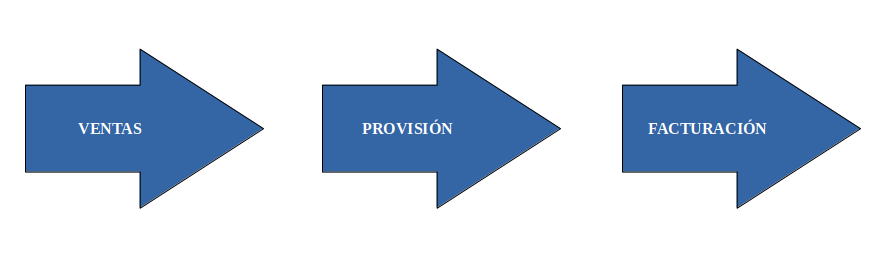
\includegraphics[width=0.50\textwidth]{imaxes/fases-proceso-negocio.png}
  \caption{Fases del proceso de negocio}
  \label{fig:fases-proceso-negocio}
\end{figure}

\begin{itemize}
\item Venta: conjunto de actividades orientadas a realizar y formalizar la venta de un servicio a través de la contratación del mismo.
\item Provisión: conjunto de actividades cuya finalidad es la de proveer el servicio previamente contratado al cliente.
\item Facturación: comprende todas las actividades destinadas a facturar la prestación de los servicios contratados y provisionados y realizar la posterior puesta a cobro de los mismos.
\end{itemize}

Como ya hemos indicado, la herramienta desarrollada para este \acrlong{tfg} se centrará en la fase de venta, concretamente la correspondiente a registrar la venta y gestionar los productos y servicios contratados así como el catálogo de productos y servicios de la empresa.


\section{Definición de objetivos}
\label{sec:objetivos}


El objetivo primordial del presente proyecto es diseñar y desarrollar una aplicación que permita gestionar el catálogo de productos y servicios de una empresa así como la cartera de clientes y sus contrataciones, para lo que se tendrán en cuenta una serie de elementos parametrizables (esto es, modificables según las necesidades del sistema) que conformarán la definición de las entidades a manejar por el sistema.

Además de realizar las diferentes altas, bajas y modificciones de los elementos que comportan el catálogo de productos y servicios y la cartera de clientes, la aplicación desarrollada deberá gestionar el histórico de datos para los elementos susceptibles de cambio y así poder reflejar los continuos cambios derivados que puedan sufrir (cambio de precio en entidades facturables, modificación del servicio contratado, cambios en las tasas impositivas, etc). También permitirá a los usuarios de la misma la gestión de su cuenta, permitiéndoles cambiar tanto la contraseña como los datos de contacto.
La herramienta a desarrollar será una aplicación web con el objetivo de disminuir el riesgo de incompatibilidades y dependencias de software así como de centralizar su distribución y posibles actualizaciones en un único punto.

Durante el desarrollo de este TFG se ha tenido en mente el sector TIC de las operadoras de telefonía, ya que, como se ha indicado anteriormente, se ha querido aprovechar el conocimiento adquirido a través de la experiencia profesional, aunque podría adaptarse a cualquier otra empresa con necesidades similares.


  \chapter{Estado del Arte}
\label{chap:estado-arte}

\lettrine{E}{l} registro de la información comercial no es algo nuevo y la forma de tratar esta información ha ido evolucionando. Y como no podía ser de otra forma la popularización de los sistemas de información supuso un salto cuantitativo a la hora de gestionar todos esos datos, desde las incipientes automatizaciones a través de las bases de datos de los 60 hasta los productos \acrshort{crm} y \acrshort{erp} comercializados hoy en día.

Existen multitud de \acrshort{crm} y \acrshort{erp} en el mercado. Nos hemos centrado en cuatro de ellas que por sus características consideramos las más relevantes, bien por su posición en el mercado o por ser una alternativa de \gls{opensource} con fuerte presencia en el sector.



\section{SalesForce CRM}
\label{sec:estado-arte-salesforce}

Salesforce CRM~\cite{SalesforceCRM} es un \acrfull{saas} por lo que, al residir en la nube permite el acceso la información en cualquier momento y desde cualquier dispositivo. Se trata de un \gls{swpropietario} cuyo modelo de negocio se basa en suscripciones de pago por uso.

El proyecto de Salesforce arrancó en 1999 y actualmente tiene su sede central en San Francisco, California (EE.UU). Fueron los primeros en lanzar un \acrshort{crm} basado en la nube y a día de hoy más de 150.000 empresas de todos los ámbitos y tamaños utilizan este producto, siendo actualmente la empresa que posee la mayor cuota de mercado de los \acrshort{crm}. \newline

Entre los \acrshort{saas} ofrecidos por el sistema Salesforce se encuentra un \acrshort{crm}, una plataforma de \emph{marketing} digital, una plataforma de servicio orientada al equipo de servicio que se complementa con redes sociales, una plataforma de comunicación para empleados, socios y clientes, una plataforma de análisis y visualización de datos y una plataforma para desarrollar aplicaciones personalizadas que se ejecutan en la plataforma Salesforce.

Entre las ventajas que ofrece se encuentran las siguientes:
\begin{itemize}
\item Facilidad de uso.
\item Consta de una amplia gama de funcionalidades.
\item Es muy personalizable.
\item Es altamente escalable.
\item Basado en tecnologías cloud.
\item Su implementación es rápida.
\end{itemize}

Entre las principales desventajas de esta solución destacan:
\begin{itemize}
\item Precio. El paquete completo de Salesforce CRM no está al alcance de todos y muchas pequeñas empresas no pueden costearlo.
\item Su exceso de funcionalidad puede suponer un inconveniente para empresas pequeñas sin equipos de ventas o marketing por ejemplo, que no podrán sacar todo el provecho a la herramienta.
\item Presenta un elevado número de actualizaciones que impactan en la interfaz, lo que en ocasiones confunde al usuario.
\end{itemize}


\section{SAP S/4HANA}
\label{sec:estado-arte-sap}

SAP~\citep{SAP} es una empresa fundada en 1972 bajo el nombre de \textit{Systemanalyse Programmentwicklung} (Desarrollo de programas de sistemas de análisis) que actualmente tiene su sede en Walldorf, Baden-Württemberg (Alemania). Con la presentación de su software original SAP R/2 y SAP R/3, SAP estableció el estándar global para el \acrlong{erp}.

En 2015 se produjo el lanzamiento de SAP S/4HANA Cloud, un software modular y completo potenciado por la inteligencia artificial y el \textit{machine learning} o aprendizaje automático. Se trata de un \gls{swpropietario} que ha sido diseñado como una solución \acrshort{erp} escalable a pequeñas, medianas y grandes empresas en función de sus objetivos y necesidades, siendo válido tanto para entornos orientados en la nube como on-premise. Esta solución es la que lidera actualmente el mercado en Europa occidental. \newline

SAP S/4HANA abarca las siguientes áreas de negocio: finanzas, gestión de activos, abastecimiento y adquisiciones, gestión de la cadena de suministros, I+D e ingeniería 


Entre las ventajas de este \acrshort{erp} se encuentran las siguientes:
\begin{itemize}
\item Es personalizable y funcional.
\item Es portable.
\item Es compatible con otras aplicaciones gracias a su programación basada en módulos funcionales.
\item Consta de una capacidad estadística bien integrada.
\end{itemize}


En cuanto a los inconvenientes de este software destacan lo siguiente:
\begin{itemize}
\item Una elevada curva de aprendizaje.
\item La implementación por módulos resulta lenta ya que suele llevarse a cabo de forma secuencial.
\item Tiene un elevado coste debido a que requiere de equipos potentes para su ejecución.
\item Tiene un elevado número de actualizaciones que suelen acarrear costes (en seguridad, almacenamiento, \dots).
\item Se requiere un gasto adiciona de personal específico para su mantenimiento.
\end{itemize}


\section{ODOO}
\label{sec:estado-arte-odoo}

Odoo~\cite{Odoo} es una empresa nacida en 2005 a partir del proyecto de de software de gestión empresarial en \gls{opensource} TinyERP cuya sede central se encuentra en Ramillies, Bélgica.

Su software Odoo es un \acrshort{erp} integrado que cuenta con una versión \textit{comunitaria} de código abierto bajo licencia LGPLv3 y una versión empresarial bajo licencia comercial que complementa la edición comunitaria y da acceso a todas las funcionalidades del producto. Su política de precios se basa en el número de usuarios y número de módulos instalados.

Se trata de un software empresarial formado por un conjunto perfectamente integrado de aplicaciones que incluye módulos para gestión de proyectos, de almacenes, ventas, comercio electrónico, facturación y contabilidad entre otros. Está disponible tanto para entornos orientados en la nube como on-premise.

Entre las ventajas de esta solución empresarial destacan las siguientes:
\begin{itemize}
\item Sus múltiples aplicaciones permiten cubrir todas las áreas de negocio de una empresa.
\item Su modularidad permite adaptar sus productos a las necesidades particulares de cada empresa
\item Su política de precios basada en el número de usuarios y módulos instalados permite \textit{pagar por lo que realmente se usa}, por lo que puede ser una gran alternativa para pequeñas empresas que no necesitan gran cantidad de aplicaciones para gestionar su negocio.
\item Cuenta con una gran comunidad de usuarios que facilita mucho la resolución de dudas. 
\item Su filosofía de \gls{opensource} lo convierte en una alternativa altamente segura, ya que es más fácil detectar vulnerabilidades en el código y corregirlas.
\end{itemize}

Algunos de los inconvenientes que presenta este producto son:
\begin{itemize}
\item Un precio mucho mayor del esperado si se requieren muchos extras o aplicaciones.
\item No existe la funcionalidad de compatibilidad de versiones, por lo que una nueva versión del producto requiere una migración de datos.
\end{itemize}



\section{ERPNext}
\label{sec:estado-arte-erpNext}
ERPNext~\cite{ERPNext} es un software \acrshort{erp} desarrollado por Frappe Technologies Pvt. Ltd, con sede en Maharashtra, India. Es un software \gls{opensource} desarrollado bajo licencia LGPLv3.

Se trata de un \acrshort{saas} configurable que consta de diferentes módulos como pueden ser \acrshort{crm}, gestión de inventario, de suscripciones, de proyectos, ventas, facturación y atención al cliente entre otros. Consta de tres planes de suscripción mensual basados principalmente en el número de usuarios y requisitos de almacenamiento necesarios.

Entre sus ventajas destacan:
\begin{itemize}
\item No existen costes de licencia.
\item La descarga es gratuita, sólo se paga por el soporte de software.
\item Es flexible y permite adaptarse a cualquier tipo de empresa, pudiendo utilizar sólo aquellos módulos que se adaptan a las necesidades de la empresa.
\item Permite la migración de datos desde el sistema local.
\end{itemize}

Entre los inconvenientes que presenta se encuentran:
\begin{itemize}
\item No es adecuado para grandes empresas.
\item Problemas de actualización con versiones personalizadas.
\item Gestión de permisos compleja.
\end{itemize}


\section{Conclusión}
\label{sec:estado-arte-conclusion}
Como hemos visto las herramientas \acrshort{crm}/\acrshort{erp} que dominan el mercado son de \gls{swpropietario} que ofrecen soluciones muy potentes que pueden ser muy ventajosas para grandes empresas, pero no así para empresas más pequeñas, las cuales no siempre se pueden permitir el coste que este tipo de software conlleva o, en caso de poder, acaban infrautilizando el software por el que están pagando, ya que las funcionalidades mínimas contratadas suelen exceder las necesidades reales de la empresa. Para estos existen herramientas de \gls{opensource} con gran presencia en el mercado en el mercado que pueden ser una buena alternativa a las soluciones de software privativo, aunque tienen el inconveniente de que suelen presentar problemas de compatibilidad de versiones.

 \chapter{Proceso de negocio. Fundamentos teóricos}
\label{chap:teoria}

\lettrine{A} { día} de hoy es innegable el papel crucial que juegan las tecnologías de la información en general y los sistemas de información en particular dentro de la gestión de procesos de negocio de cara a la consecución de objetivos de forma eficaz y eficiente. 

El mercado está en continua evolución. Los sistemas de información nos proporcionan la tecnología básica necesaria tanto para crear nuevas funcionalidades como para adaptar las existentes para poder satisfacer las nuevas necesidades que van surgiendo. 

Este capítulo pretende ser una aproximación a los conceptos teóricos en los que se enmarcan los procesos empresariales dentro del sector \acrfull{tic}.


\section{Proceso de negocio}

Hammer \& Champy (1993)~\cite{Hammer-Champy} definieron el proceso de negocio como:

\begin{displayquote}
Una colección de actividades que toman uno o más tipos de entradas y crean una salida que tiene valor para el cliente. 
\end{displayquote}

Así pues, podemos entender un proceso de negocio como un conjunto de funciones dentro de una secuencia específica que proporciona valor a un cliente interno o externo y cada función dentro de un proceso puede ser a su vez interpretado como un proceso en si mismo llamado sub-proceso. El desencadenante de este subproceso es el proceso previo (o por el evento inicial que da comienzo al proceso en general) y devuelve un resultado de valor para el siguiente proceso o para el cliente final y sus procesos si este es el último suproceso de un proceso de extremo a extremo~\cite{Kirchmer}. 

Esta descomposición de procesos en subprocesos puede extenderse tanto como las funciones resultados sigan teniendo sentido desde el punto de vista de negocio: por ejemplo el subproceso "gestión de ventas" puede describirse en detalle usando funciones como "registro de orden de venta" o "asignación de productos a la orden de venta", sin embargo descomponer la función "registro de orden de venta" en actividades como "introducir nombre de cliente", "introducir dirección de cliente", etc. no aportan relevancia alguna desde el punto de vista de negocio.

Con el objetivo de poder definir de forma sencilla los procesos más complejos sin dejar de lado ningún aspecto importante de los mismos surge la \acrfull{aris}, una aproximación al proceso de arquitectura y modelado empresarial desarrlollado por August-Wilhem Scheers y que permite describir un proceso de negocio desde cinco puntos de vista diferentes, dando respuesta a todas las cuestiones relevantes relativas al proceso:

\begin{itemize}
\item Vista organizacional: ¿quién (gente, departamentos, empresas, etc.) está involucrado en el proceso?
\item Vista funcional: ¿qué funciones se llevan a cabo dentro del proceso?
\item Vista de datos: ¿qué datos o información es necesaria/producida para/en el proceso?
\item Vista de entrega: ¿qué son los entregables del proceso y por qué los necesito?
\item Vista de control: el cómo se ve en conjunto refleja el quién está haciendo qué, qué datos producen entregables y cual es la secuencia lógica que hace que las funciones lleven a cabo su función.
\end{itemize}


La figura ~\ref{fig:aris} (página~\pageref{fig:aris})  muestra la arquitectura \acrshort{aris}:


\begin{figure}[H]
  \centering
  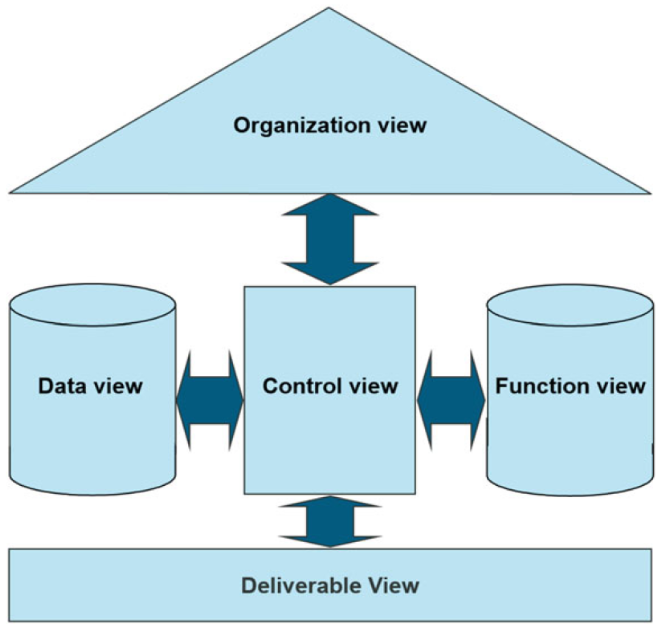
\includegraphics[width=0.30\textwidth]{imaxes/aris.png}
  \caption{Arquitectura de sistema de información integrada (\acrshort{aris})}
  \label{fig:aris}
\end{figure}


El elemento más importante de la arquitectura \acrshort{aris} es la vista de control. Esta muestra como dos o más aspectos de un proceso \textit{encajan}, por ejemplo quién es responsable de una función determinada o qué función usa determinados datos. La vista resultado de la integración de varios aspectos del proceso de negocio es la llave para la gestión exitosa de dichos procesos. \acrshort{aris} ayuda a convertir los procesos en algo \textit{tangible} al definir cómo describirlos asentando la base para convertir la \acrlong{bpm} en una disciplina de gestión real.


\subsection{Gestión de proceso de negocio}

Un \acrfull{bpm} incluye conceptos, métodos y tecnicas para soportar el diseño, la administración, la configuración, la representación y el análisis de los procesos de negocio~\cite{Weske}.

La base del \acrshort{bpm} es la representación explícita de los procesos de negocio con sus actividades y las restricciones de ejecución de los mismos.


El ciclo de vida del \acrshort{bpm} consta de cinco fases~\cite{bpmLifecycle} tal y como se muestra en la figura ~\ref{fig:lifecycle-bpm} (página~\pageref{fig:lifecycle-bpm}):


\begin{figure}[hp!]
  \centering
  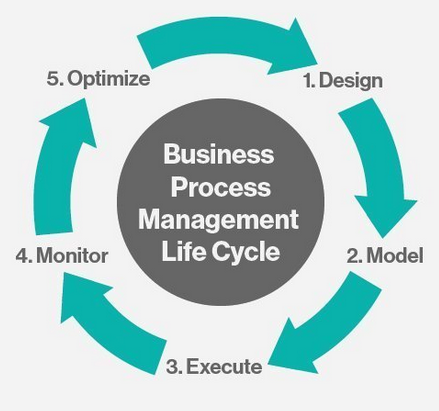
\includegraphics[width=0.30\textwidth]{imaxes/bpm-lifecycle.png}
  \caption{Ciclo de vida del \acrshort{bpm}}
  \label{fig:lifecycle-bpm}
\end{figure}

\begin{enumerate}
\item Diseño: el diseño de procesos abarca tanto la identificación de procesos existentes como el diseño de procesos "futuros". El objetivo de este paso es garantizar un diseño correcto y eficiente. Debe haber una sincronización entre los procesos existentes y el diseño de un nuevo proceso para evitar posibles interrupciones.
\item Modelado: se crea una representación visual del modelo de proceso. Esto debe incluir detalles específicos, como líneas de tiempo, descripciones de tareas y cualquier flujo de datos en el proceso. 
\item Ejecución: consiste en una prueba de concepto, probando el nuevo sistema BPM con un grupo limitado. Después de incorporar cualquier comentario, el equipo puede comenzar a implementar el proceso a un público más amplio.
\item Supervisión:  durante esta etapa, se supervisa el proceso, se miden las mejoras en la eficiencia y se identifica cualquier cuello de botella adicional.
\item Optimización: se realizan los ajustes finales al proceso para mejorar la actividad empresarial.

\end{enumerate}

Entre las ventajas que proporcionan los \acrshort{bpm} se encuentran las siguientes:

\begin{itemize}
\item Mayor eficiencia y ahorro de costes: gracias a la optimización de los procesos existentes y a la incorporación de más estructura en el desarrollo de nuevos procesos, eliminando redundancias y cuellos de botella.
\item Mejor experiencia de empleados y clientes: ya que permite eliminar el trabajo repetitivo y aumentar la accesibilidad de la información mejorando la productividad y la implicación con el cliente.
\item Procesos más escalables: a través de la mejora en la ejecución de procesos y la automatización de flujos de trabajo se facilita el escalado de procesos a otras zonas geográficas de todo el mundo.
\item Mayor transparencia: puesto que la automatización de procesos de negocio define claramente a los propietarios para las tareas a lo largo del proceso, se proporciona más transparencia y responsabilidad a lo largo de un proceso determinad, favoreciendo la comunicación entre equipos.
\end{itemize}




\section{Sistemas de soporte operacional y Sistemas de soporte de negocio}

Centrándonos en el área de las telecomunicaciones, nos encontramos con dos nuevos conceptos:


\acrfull{oss}. Se trata de un término usado para describir los sistemas de procesado de información utilizados por las operadoras para gestionar sus redes de comunicación. Originalmente conocidas como herramientas de Gestión de redes de telecomunicaciones o Telecommunication Network Management tools actualmente estas soluciones son mucho más sofisticadas, permitiendo coordinar clientes, servicios, recursos, procesos y actividades. Ayudan a las operadoras a diseñar, construir, operar y mantener las redes de comunicaciones.

\acrfull{bss} es el término tradicionalmente utilizado para describir las funcionalidades de negocio y/o orientada al cliente. Estas herramientas  permiten que una organización contacte con sus clientes (por ejemplo a través del \acrshort{crm}), crear ofertas para ellos, emitir facturas así como transacciones entre operadores de comunicaciones (liquidaciones, punto de interconexión).

De forma conjunta \acrshort{oss} y \acrshort{bss} permiten a los operadores de red ofrecer servicios de manera eficiente y confiable a un enorme número de suscriptores en algunas de las máquinas más complejas del mundo, las redes globales de telecomunicaciones.

Existen distintos estándares para aportar consistencia entre las distintas aplicaciones existentes. Comentaremos brevemente algunas de ellas.

\subsection{TMN de ITU-T}

Las Comisiones de Estudio del \acrfull{itut} reúnen a expertos de todo el mundo para elaborar documentos de especificación de telecomunicaciones y protocolos informáticos, conocidos como Recomendaciones ITU-T, que actúan como elementos definitorios de la infraestructura mundial de las \acrfull{tic}  ~\cite{ITU-T}. 

Los esfuerzos de normalización de la \acrshort{itut} comenzaron en 1865 con la formación de la International Telegraph Union (en español Unión Telegráfica Internacional), que más tarde se convirtió en la \acrfull{itu}. La \acrshort{itu} se convirtió en un organismo especializado de las Naciones Unidas en 1947. El \acrfull{ccitt} fue creado en 1956, y pasó a llamarse \acrshort{itut} en 1993.


El modelo tecnológico \acrshort{tmn} se presenta en la recomendación M.3010 y suele referenciarse como la pirámide \acrshort{tmn} (figura ~\ref{fig:pirámide-tmn}, página~\pageref{fig:pirámide-tmn}). Aborda la complejidad de la gestión de las telecomunicaciones a través de una arquitectura lógica por capas, la cual organiza las funciones en grupos denominados capas lógicas y describe las relaciones entre las mismas. Una capa lógica refleja aspectos particulares de la gestión e implica el agrupamiento de la información de gestión relativa a ese aspecto. Estas capas son las siguientes:

\begin{itemize}
\item Capa de gestión de elementos. Proporciona definición y coordinación de una colección de dispositivos de red, aunque sea un subconjunto de toda la red. Esta capa normalmente incluiría la consolidación de la administración de alarmas, la copia de seguridad, el registro y el mantenimiento de los sistemas que admiten los dispositivos de red.
\item Capa de gestión de red. Proporciona la vista de administración general de la red como una suma de partes componentes. Es responsable de la supervisión, configuración y control de extremo a extremo de la red.
\item Capa de gestión de servicios. Responsable de definir los servicios ofrecidos por las operadoras de comunicaciones. Esto proporciona la interfaz entre los servicios de un cliente y la red, incluyendo la definición, la administración y la carga.
\item Capa de gestión empresarial. Representa la funcionalidad relacionada con la planificación estratégica del negocio, como las tendencias, la calidad, etc., y proporciona la base para la facturación, el presupuesto y el establecimiento de objetivos.
\end{itemize}


\begin{figure}[H]
  \centering
  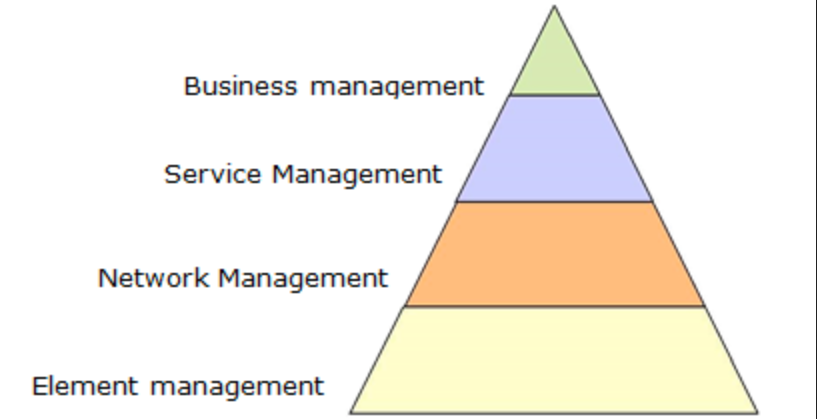
\includegraphics[width=0.40\textwidth]{imaxes/piramide-tmn.png}
  \caption{Modelo tecnológico \acrshort{tmn}}
  \label{fig:pirámide-tmn}
\end{figure}


Las áreas funcionales de gestión presentadas en la recomendación M.3400 incluyen entre otras las siguientes áreas: 
\begin{enumerate}
\item Administración de clientes.
\item Gestión de aprovisionamiento de red.
\item Administración de tarifas, cobros y contabilidad.
\item Administración de Medición y Análisis de Tráfico
\item Gestión del tráfico.
\item Administración de Enrutamiento y Análisis de Dígitos
\item Administración de Seguridad.
\end{enumerate}


\subsection{TMF}

\acrlong{tmf} es una alianza compuesta por más de 850 compañías globales que trabajan conjuntamente proporcionando un entorno abierto y colaborativo y un soporte práctico que permite a las compañías proveedoras de servicios y sus distribuidores transformar rápidamente sus operaciones comerciales, sistemas de TI y ecosistemas para capitalizar las oportunidades presentadas en un mundo digital en rápida evolución~\cite{TMFORUM}.

\acrshort{tmf} fue fundada como OSI/Network Management Forum (en español Foro de Gestión de Redes/OSI) en 1988 por ocho empresas para resolver de forma conjunta los problemas de gestión operativa y de sistemas con los protocolos OSI. En 1998 el nombre fue cambiado a TeleManagement Forum. En 2008, la organización cambió su nombre a TM Forum.

A través de estas colaboraciones los modelos de \acrshort{tmn} han ganado un uso generalizado en el campo de las implementaciones de OSS. Dentro de los trabajos desarrollados por el \acrshort{tmf} encuentra el Frameworx. Se trata un marco de arquitectura empresarial orientado a los proveedores de servicios de comunicaciones que consta de 4 marcos de trabajo o frameworks:

\begin{enumerate}
\item Un modelo de aplicación (\acrfull{tam}). Proporciona un marco modular de bloques funcionales de gestión. Esto ayuda a proporcionar una mayor consistencia (y compatibilidad) entre los conjuntos de productos de diferentes proveedores (figura ~\ref{fig:tam}, página~\pageref{fig:tam}).
\item Un modelo de proceso (\acrfull{etom}). Tiene como objetivo proporcionar un lenguaje común y un catálogo de procesos de negocio utilizados en entornos de telecomunicaciones. Este nivel de normalización tiene por objeto simplificar las líneas de comunicación entre los proveedores de servicios y los integradores de sistemas asociados (figura ~\ref{fig:etom}, página~\pageref{fig:etom}).
\item Un modelo de información (\acrfull{sid}). Su objetivo es definir las entidades esenciales, las relaciones y los atributos de los objetos de datos que prevalecen en las aplicaciones/bases de datos de telecomunicaciones. También proporciona un lenguaje común para su uso por los desarrolladores/integradores de OSS. (\acrshort{tmf}) también ha tratado de desarrollar API estandarizadas basadas en SID (interfaces de programación de aplicaciones) como OSS/J para acelerar la integración de sistemas dispares.
\item Un marco de integración de sistemas (\acrfull{tna}). Tiene como objetivo proporcionar estandarización arquitectónica, sin dejar de ser tecnológicamente neutral, incluyendo interfaces, mecanismos y políticas comunes. La integración también se conoce comúnmente como el (\acrfull{tip})
\end{enumerate}

\begin{figure}[H]
  \centering
  \begin{subfigure}[c]{0.3\textwidth}
    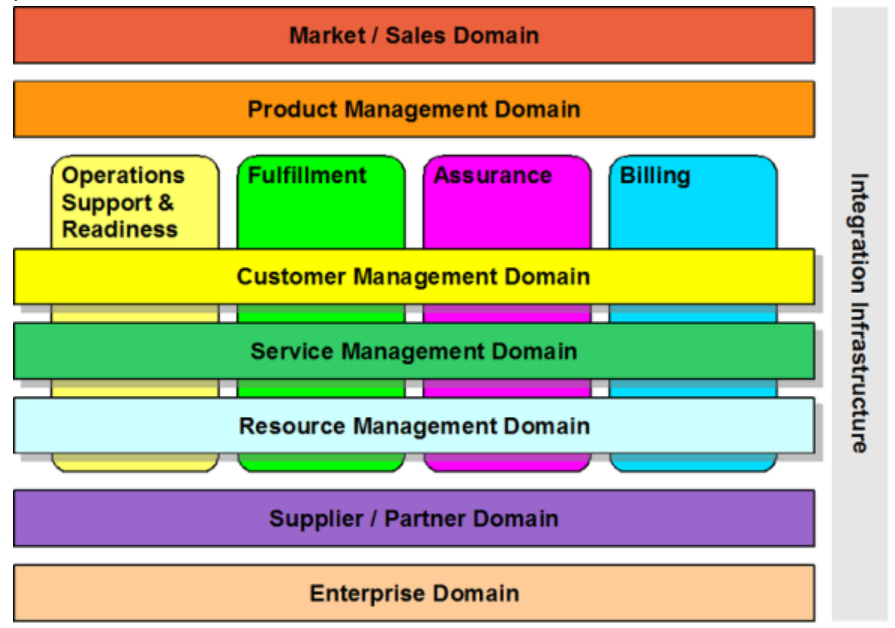
\includegraphics[width=\textwidth]{imaxes/tam.png}
    \caption{Modelo de proceso \acrshort{tam}}
    \label{fig:tam}
  \end{subfigure}
  \hspace{0.1\textwidth}
  \begin{subfigure}[c]{0.3\textwidth}
    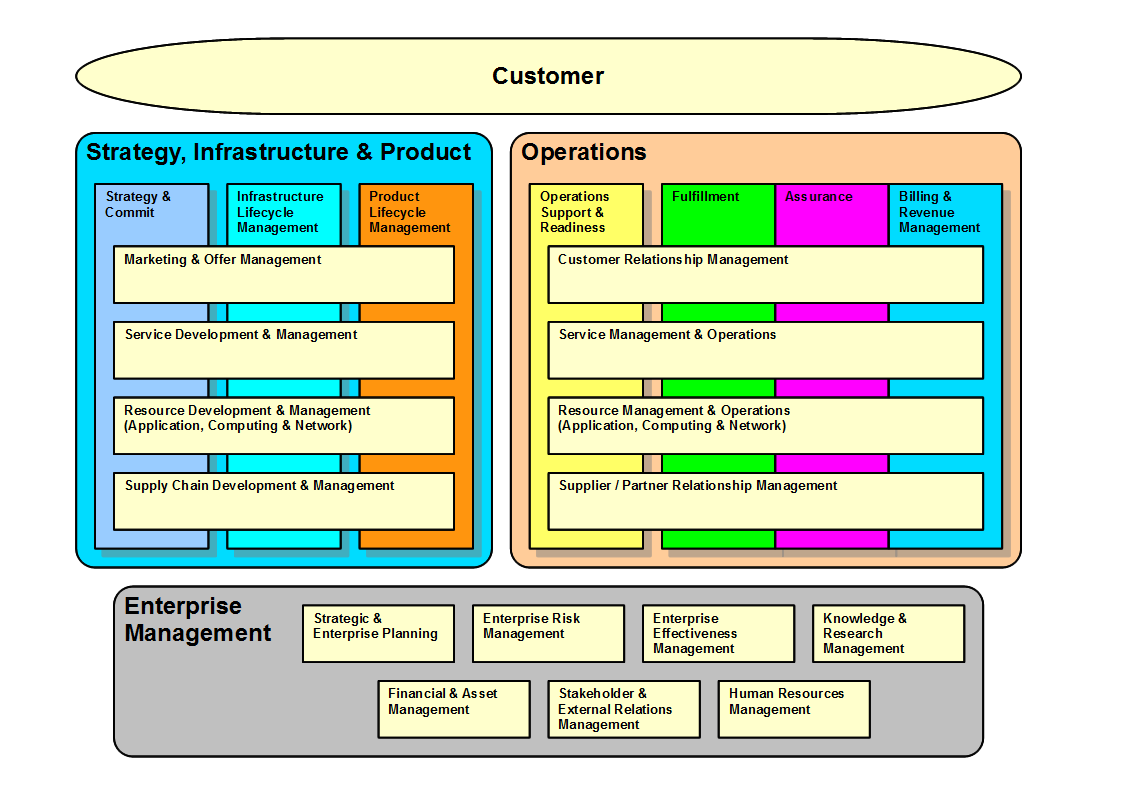
\includegraphics[width=\textwidth,height=3cm]{imaxes/etom.png}
    \caption{Modelo de proceso \acrshort{etom}}
    \label{fig:etom}
  \end{subfigure}
  \caption{Modelos de referencia del marco de trabajo de \acrshort{tmn}}
  \label{fig:tam-etom}
\end{figure}


Además de estos marcos de trabajo (\acrshort{tmf}), el (\acrlong{tmf}) cuenta con la suite TM Forum Open API, que tiene más de 50 API basadas en REST (y muchas más en desarrollo) y con un el (\acrfull{oda}), un estándar en evolución que tiene la intención de establecer una nueva visión para \acrshort{oss}/\acrshort{bss} que parecen estar ganando uso generalizado en el mundo de las telecomunicaciones.


\subsection{ITIL e ITSM}

\acrfull{itil} describe procesos, procedimientos, tareas y listas de verificación que no son ni específicos de la organización ni de la tecnología, pero que pueden ser aplicados por una organización hacia la estrategia, la entrega de valor y el mantenimiento de un nivel mínimo de competencia. Se creó originalmente en la década de 1980 como una colección de libros, cada uno de los cuales cubría una práctica específica de gestión de servicios de \acrshort{ti}. Fue desarrollado por el Gobierno del Reino Unido en un intento de estandarizar los procesos de \acrshort{ti}, en particular el traspaso de la implementación a los entornos de soporte de \acrshort{ti} en curso. Entre 1986 y 1996, esta colección aumentó a más de 30 volúmenes. Durante los años 2000 y 2001 estos volúmenes se consolidaron en 9 conjuntos que agrupaban temas relacionados~\cite{Exin, ItilWiki}. 


\acrfull{itsm} es un conjunto de políticas, procesos y procedimientos para gestionar la implementación, mejora y soporte de servicios de \acrshort{ti} orientados al cliente. A diferencia de otras prácticas de gestión de \acrshort{ti} que se centran en hardware, redes o sistemas, \acrshort{itsm} es un enfoque más centrado en los procesos y las personas, teniendo como objetivo la mejora constante el servicio al cliente de \acrshort{ti} de forma alineada a los objetivos comerciales. Las empresas que utilizan \acrshort{itsm} consideran la \acrshort{ti} como un servicio, con un enfoque en la prestación de servicios valiosos a los clientes, en lugar de un departamento que administra la tecnología.

Los principales elementos de \acrshort{itsm} son:

\begin{itemize}
\item Gestión de incidencias.
\item Gestión de problemas. 
\item Gestión del cambio. 
\item Gestión de proyectos. 
\item Gestión de activos. 
\item Conocimiento, política y procedimiento. 
\item Catálogo de servicios. 
\item \textit{Service Desk.}
\end{itemize}

Aunque a veces se usan indistintamente, \acrshort{itsm} e \acrshort{itil} no son lo mismo: \acrshort{itil} es uno de los marcos más populares dentro de la disciplina \acrshort{itsm}, y ha ayudado a informar e inspirar otros marcos \acrshort{itsm}. Por lo tanto \acrshort{itil} es la base en la que se apoya \acrshort{itsm} proporcionando a las empresas la metodología necesaria para adoptar e implementar \acrshort{itsm} (figura ~\ref{fig:itil-vs-itsm},  página~\pageref{fig:itil-vs-itsm})

\begin{figure}[H]
  \centering
  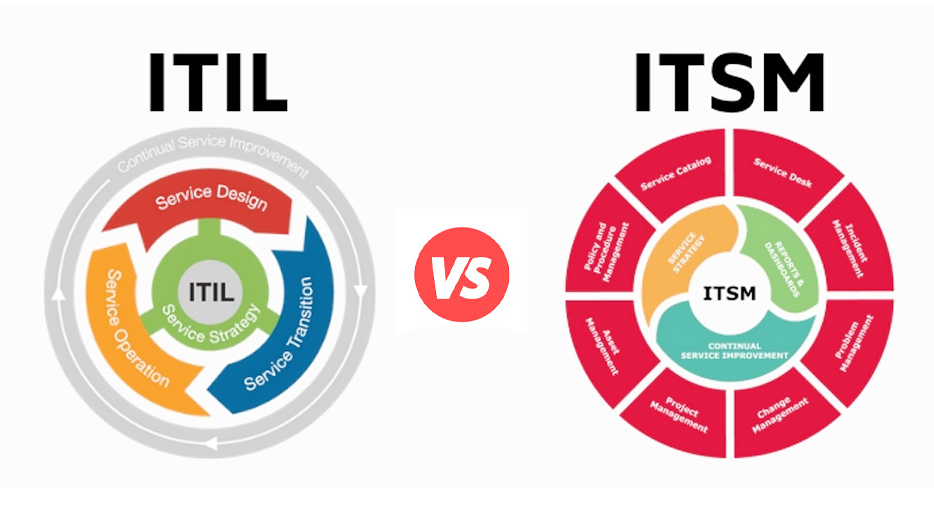
\includegraphics[width=0.30\textwidth]{imaxes/itil-vs-itsm.png}
  \caption{ \acrshort{itil} y \acrshort{itsm}}
  \label{fig:itil-vs-itsm}
\end{figure}



Por otro lado, de la misma forma que existe una una superposición cada vez mayor entre las \acrshort{ti} y las tecnologías de redes de telecomunicaciones, también hay una mayor prevalencia de marcos de \acrshort{ti} (como \acrshort{itil}) que se utilizan junto con los marcos de telecomunicaciones (como \acrshort{etom}). Los proveedores de servicios de telecomunicaciones dependen de una infraestructura de TI altamente confiable (por ejemplo, servidores, etc.) e ITIL se considera actualmente como la mejor práctica para la gestión de este tipo de activos. Del mismo modo, los clientes están subcontratando la gestión de la infraestructura de TI y telecomunicaciones de extremo a extremo, exigiendo a sus proveedores de servicios que suministren una gestión de servicios de alta calidad de la red y los activos de TI cada vez más críticos del cliente.


\acrshort{etom} comparte algunos puntos en común y varias diferencias con \acrshort{itil}. \acrshort{tmf} ha publicado una nota de aplicación eTOM – ITIL (GB921L) titulada "Using eTOM to model the ITIL Processes". Esta nota proporciona orientación sobre el modelado de la gestión de servicios de \acrshort{ti} utilizando los elementos de proceso estándar dentro de \acrshort{etom} así como una superposición detallada de procesos \acrshort{itil} con procesos \acrshort{etom} (figura ~\ref{fig:itil-etom}, página~\pageref{fig:itil-etom})



\begin{figure}[H]
  \centering
  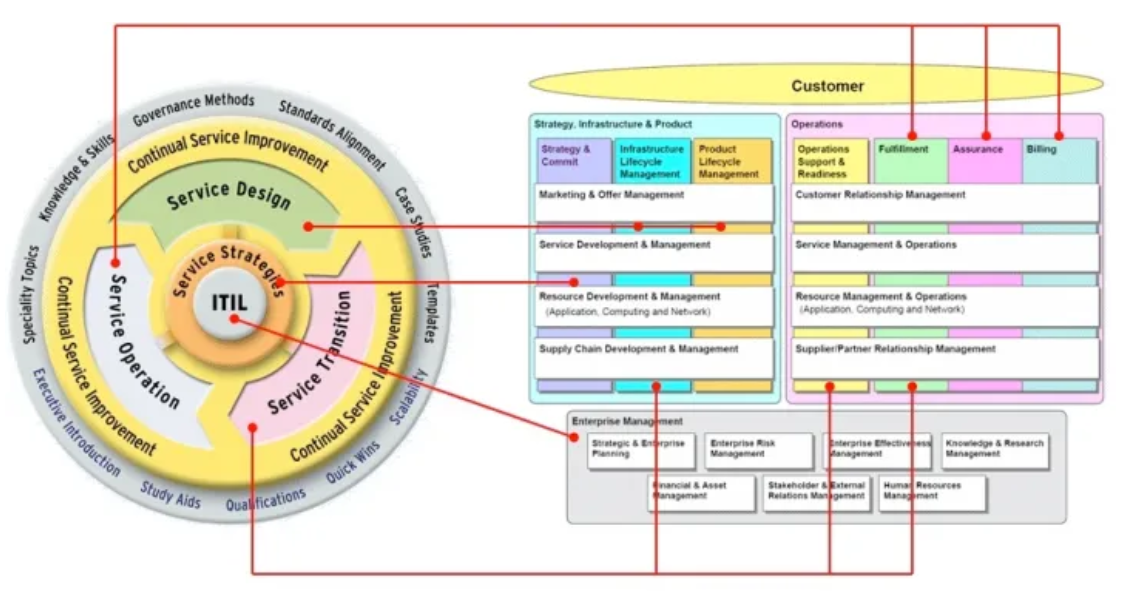
\includegraphics[width=0.30\textwidth]{imaxes/etom-itil.png}
  \caption{Aproximación al mapeo entre \acrshort{etom} e \acrshort{itil}~\cite{Itil-eTom}}
  \label{fig:itil-etom}
\end{figure}


\section{Gestión de relaciones con los clientes}


La \acrfull{crm} es una estrategia comercial que optimiza los ingresos y la rentabilidad al tiempo que promueve la satisfacción y la lealtad del cliente. Las tecnologías CRM permiten la estrategia, e identifican y gestionan las relaciones con los clientes~\cite{GartnerCRM}. El compendio de conceptos, procedimientos y reglas que una corporación sigue al comunicarse con sus consumidores se conocen como  \acrshort{crm}~\cite{WikiCRM} y por definición cubre todas las formas en las que se administran las relaciones con los clientes en los distintos ámbitos empresariales: ventas, marketing, servicio al cliente y comercio electrónico~\cite{SAP-CRM} . 

Por lo general, cuando hablamos de \acrshort{crm} estamos refiriéndonos a los sistemas de software que nos ayudan a construir estrategias de negocio para retener y captar clientes.
El software \acrfull{crm} permite automatizar e integrar estas actividades orientadas al cliente e incluso pueden ofrecer herramientas para el análisis de clientes, la personalización, las redes sociales, la colaboración y mucho más. La funcionalidad que el software \acrshort{crm} proporciona a las empresas se divide en cuatro segmentos: ventas, marketing, servicio al clientes y comercio digital~\cite{GartnerCRM}. 


\subsection{Breve historia del CRM}

La necesidad de mantener registros relativos a la información comercial no es algo nuevo. De hecho podríamos decir que existe desde que existe el comercio: con el tiempo el saber quien poseía qué o quien debía a quién requiería alguna forma de notación y registro permanente, así como alguna forma de contabilidad para la gestión de los bienes. El tratamiento de esta información fue evolucionando adaptándose a las necesidades que iban surgiendo en cada momento como pudiera ser la segmentación de clientes atendiendo a sus capacidad de pago o a su nivel económico, permitiendo aplicar distintas estrategias comerciales en función de la información almacenada. 


La aparición del Rodolex (palabra compuesta a partir de las palabras \textit{rolling} e \textit{index}) en la década de los 50 (figura ~\ref{fig:rodolex} , página~\pageref{fig:rodolex}) supuso un gran avance en el tratamiento de los clientes. Este dispositivo giratorio que permitía almacenar tarjetas indexadas de quita y pon que contenían la información relevante de distintas personas y empresas, resultó ser una forma mucho más rápida, cómoda y eficaz de acceder y/o modificar dicha información que los métodos existentes hasta el momento (principalmente la búsqueda de información en libros de contabilidad y archivos personales del cliente). Este término se ha vuelto algo genérico para nombrar cualquier organizador personal que realice esta función, o como una metonimia para el total de los contactos comerciales acumulados de un individuo.


\begin{figure}[H]
  \centering
  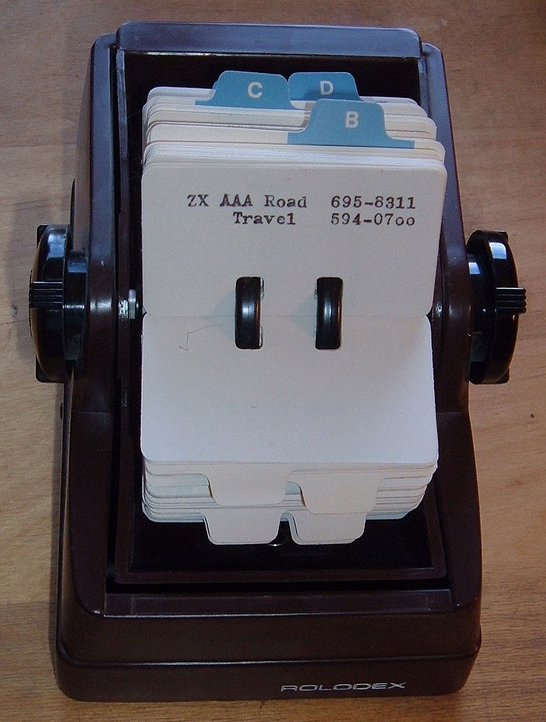
\includegraphics[width=0.3\textwidth]{imaxes/rodolex.png}
  \caption{Rodolex}
  \label{fig:rodolex}
\end{figure}




En la década de los 60 comienza la introducción de las computadoras en las empresas. Los sistemas de mainframe independientes se hicieron ampliamente disponibles para las empresas lo que les permitiría manejar bases de datos de los clientes y aplicar un nivel (básico) de automatización, ayudando a mantener registros contables. Inicialmente la gestión de clientes pertenecía al departamento de cuentas, pero esta automatización pronto se extendió a otros departamentos, incluidos ventas y marketing. En la década de los 70 el precio de los ordenadores disminuyó drásticamente, lo que permitió que hasta las pequeñas empresas se sumaran al carro de la revolución informática y a partir de ahí vino la siguiente evolución del CRM.


Los inicios del CRM tal como lo conocemos comenzaron en la década de 1980. En esta época se produzco el cámbio del márketing directo al márketing de base de datos. Esto marca el comienzo de la combinación de datos de clientes con estrategia de ventas, una parte central de CRM tal como lo conocemos hoy~\citep{ThinkautomationCRM}:

\begin{itemize}
\item Marketing directo: Cualquier práctica de marketing que implique comunicación directa o interacción con clientes individuales. Por ejemplo, a través de la comunicación postal directa como catálogos y cartas.
\item Marketing de base de datos: Una forma de marketing directo que implica recopilar datos de clientes, analizar estos datos y usarlos para crear mensajes de marketing personalizados y predecir las acciones y deseos de nuevos clientes potenciales. Se trata de utilizar datos para optimizar los esfuerzos de marketing.
\end{itemize}


Robert y Kate Kestnbaum fueron pioneros del marketing de bases de datos. Se trataba de una forma de marketing directo que analizaba estadísticamente la base de datos de clientes para identificar qué clientes tendrían más probabilidades de reaccionar a una campaña de marketing. El concepto despegó y Kestnbaum, junto con Robert Shaw, nos trajo nuevos conceptos y metodologías, que van desde el valor de por vida del cliente hasta la gestión del canal. En 1986, Pat Sullivan y Mike Muhney lanzaron un sistema de evaluación de clientes llamado ACT! (acrónimo de "Automated Contact Tracking" - Seguimiento automatizado de contactos en español) basado en el principio de Rolodex digital, que ofrecía por primera vez un servicio de gestión de contactos que facilitaba el almacenamiento de información de contactos (nombres, direcciones, números de teléfono, etc.), lo que podría considerarse como el primer CRM automatizado~\cite{SalesforceCRM}. 


A medida que las oficinas se digitalizaron a lo largo de la década de 1990 surgieron una gran cantidad de nuevos productos de gestión de datos de clientes. Estos productos se definían como \acrfull{sfa} y eran una amalgama de márketing de base de datos y gestión de contactos. En 1993, Tom Siebel diseñó el primer producto de \acrshort{crm}, Siebel Customer Relationship Management. Con el fin de competir con estas novedosas soluciones de \acrshort{crm}, las empresas de \acrfull{erp}\footnote{\acrshort{erp}: sofware que se ocupa de la gestión de los principales procesos comerciales, incluidas las áreas relacionadas con las relaciones con los clientes} también vieron una oportunidad y el mercado se volvió muy competitivo. A mediados de los años 90, este mercado se disparó en ofertas de productos de todas las formas y tamaños, ahora conocidas como sistemas \acrshort{crm}. La gestión de relaciones con los clientes se popularizó en 1997, debido al trabajo de Siebel, Gartner e IBM. Entre 1997 y 2000, los principales productos de \acrshort{crm}. se enriquecieron con capacidades de envío y marketing. Siebel introdujo la primera aplicación de \acrshort{crm}. móvil llamada Siebel Sales Handheld en 1999. La idea de una base de clientes independiente y alojada en la nube pronto fue adoptada por otros proveedores líderes en ese momento, incluidos PeopleSoft (adquirido por Oracle), Oracle, SAP y Salesforce.com.

Y así llegamos a nuestros días, en los que el mercado de nuevos productos \acrshort{crm} no parece haber alcanzado su punto de saturación. Las nuevas empresas continúan llegando al mercado con productos en la nube, mientras que los proveedores existentes han cambiado sus modelos de licencia para ofrecer alternativas en la nube a las licencias de sitios tradicionales. El último cambio es el aumento de los datos sociales y la necesidad de interactuar con los clientes en las diversas plataformas sociales. El móvil se ha vuelto aún más imperativo como una oferta con la llegada del teléfono inteligente. El ritmo del cambio es tan rápido que muchos proveedores están luchando para mantenerse al tanto de los últimos desarrollos, que van desde chatbots hasta big data e IA. Si bien se podría esperar que los productos de \acrshort{crm} hayan madurado, los clientes aún experimentan dificultades para lograr implementaciones exitosas. Esto se debe a que ellos también están luchando por mantener sus modelos de negocio relevantes y sostenibles en esta era disruptiva.

 \chapter{Fundamentos Técnicos}
\label{chap:fmtos-técnicos}


\lettrine{E}{n} este capítulo introduciremos las diferentes tecnologías usadas en el desarrollo del presente \acrshort{tfg}.


\section{Jakarta EE}
\label{sec:jakartaEE}


\acrfull{jee} es un conjunto de especificaciones que amplía \acrfull{jse} con especificaciones propias de características empresariales como pueden ser la informática distribuida y los servicios web. Las aplicaciones de \acrshort{jee} manejan las transacciones, seguridad, escalabilidad, concurrencia y administración de los componentes que está implementando. Algunas áreas en las que se utiliza \acrshort{jee} son el comercio electrónico, la  contabilidad o los sistemas de información bancaria.

Jakarta EE ofrece a los desarrolladores un conjunto completo de especificaciones abiertas y neutrales para proveedores que se utilizan para desarrollar aplicaciones Java modernas y nativas desde cero tanto en servidores locales como residentes en la nube. Ofrece una combinación de ventajas que no se pueden encontrar en otros marcos Java: madurez, estabilidad y retrocompatibilidad. Su flexibilidad arquitectónica permite arquitecturas de microservicios basadas en la nube, así como arquitecturas tradicionales y monolíticas. Se trata de una plataforma con todas las funcionalidades que se puede configurar con unas pocas líneas de código y presenta la capacidad de poder cambiar fácilmente las tecnologías subyacentes para cumplir con los nuevos requisitos y aprovechar las implementaciones más rápidas y ligeras~\cite{JakartaEE-eclipse}. 


\subsection{Historia}
\label{sec:historia}

El lenguaje de programación Java nació en 1991 de la mano de James Gosling, que en aquellos momentos trabajaba en Sun Microsystems, y su equipo. Los objetivos de Gosling eran implementar una máquina virtual y un lenguaje con una estructura y sintaxis similar a C++. La promesa inicial de Gosling era  \textquote{\textit{Write Once, Run Anywhere}} (Escríbelo una vez, ejecútalo en cualquier lugar), proporcionando un lenguaje independiente de la plataforma y un entorno de ejecución ligero y gratuito para las plataformas más populares (la \acrfull{jvm}), de forma que los binarios (\emph{bytecode}) de las aplicaciones Java pudiesen ejecutarse en cualquier plataforma. En 1995 fue lanzado comercialmente por Sun Microsystems como un componente fundamental de la plataforma Java. 

La plataforma Java es un conjunto de programas que facilitan el desarrollo y la ejecución de programas escritos en el lenguaje de programación Java. Una plataforma Java incluye un motor de ejecución (la \acrshort{jvm}), un compilador y un conjunto de bibliotecas. También puede haber servidores adicionales y bibliotecas alternativas que dependen de los requisitos. Las plataformas Java se han implementado para una amplia variedad de hardware y sistemas operativos con el fin de permitir que los programas Java se ejecuten de manera idéntica en todos ellos. Existen distintas plataformas orientadas a distintas clases de dispositivos y aplicaciones, a saber:
\begin{itemize}
\item Java Card: Una tecnología que permite que las pequeñas aplicaciones basadas en Java (applets) se ejecuten de forma segura en tarjetas inteligentes y dispositivos similares de pequeña memoria. 
\item Java ME (Micro Edition): especifica varios conjuntos diferentes de bibliotecas (conocidas como perfiles) para dispositivos con capacidades limitadas de almacenamiento, visualización y energía. A menudo se utiliza para desarrollar aplicaciones para dispositivos móviles, PDA, decodificadores de TV e impresoras. 
\item \acrshort{jse} (\acrlong{jse}): Para uso general en PC de escritorio, servidores y dispositivos similares. 
\item \acrshort{jee} (\acrlong{jee}): conjunto de \acrshort{jse} junto a varias \acrfull{api} que son útiles para aplicaciones empresariales cliente-servidor de varios niveles.
\end{itemize}


Puesto que el desarrollo de este trabajo ha sido a través de \acrshort{jee}, nos centraremos en dicha plataforma. Java Enterprise Edition fue un proyecto iniciado por Sun Microsystems en el año 1999 bajo el nombre de J2EE y adquirida por Oracle diez años más tarde, dando continuidad al proyecto hasta 2017, momento en el que el proyecto pasó a manos de la Eclipse Foundation, quien continúa con su desarrollo bajo la modalidad de código abierto en la actualidad ~\cite{JakartaEE-eclipse}.

Esta transferencia de proyecto de Oracle a Eclipse Foundation no incluyó el uso de la marca Java, por lo que Eclipse Foundation renombró el proyecto pasando a denominarse \acrshort{jee}. La primera versión lanzada bajo el paraguas de Eclipse Foundation fue la 8 (versión con la que se ha desarrollado la aplicación de este \acrshort{tfg}) y actualmente está disponible la versión 9.1. La \tablename~\ref{tab:evolucionJavaEE} muestra la evolución histórica de Java EE y Jakarta EE.

\begin{table}
  \centering
  \rowcolors{2}{white}{udcgray!25}
  \begin{tabular}{c|c|c|c}
  \rowcolor{udcpink!25}
  \textbf{Versión} & \textbf{Año} & \textbf{Soporte Java SE} & \textbf{Empresa}\\
J2EE 1.2 & 1999 & J2SE 1.2 & Sun Microsystems \\
J2EE 1.3 & 2001 & J2SE 1.3 & Sun Microsystems \\
J2EE 1.4 &2003 & J2SE 1.4 & Sun Microsystems \\
Java EE 5 & 2006 & Java SE 5 & Sun Microsystems \\
Java EE 6 & 2009 & Java SE 6 & Oracle \\
Java EE 7 & 2013 & Java SE 7 & Oracle \\
Java EE 8 & 2017 & Java SE 8 & Oracle \\
Jakarta EE 8 & 2019 & Java SE 8 & Eclipse Foundation \\
Jakarta EE 9 & 2020 & Java SE 8 & Eclipse Foundation \\
Jakarta EE 9.1 & 2021 & Java SE 11//Java SE 8 & Eclipse Foundation \\
  \end{tabular}
  \caption{Evolución de Java EE}
  \label{tab:evolucionJavaEE}
\end{table}



\subsection{Arquitectura Jakarta EE}
\label{sec:arquitectura}


\acrshort{jee} se define por su especificación. La especificación define las \acrfull{api} y sus interacciones. \acrshort{jee} incluye varias especificaciones que sirven para diferentes propósitos, como pueden ser generar páginas web, leer y escribir desde una base de datos de manera transaccional, administrar colas distribuidas. Las \acrshort{api} de \acrshort{jee} incluyen varias tecnologías que amplían la funcionalidad de las \acrshort{api} de Java SE base, como Jakarta Enterprise Beans, conectores, servlets, Jakarta Server Pages y varias tecnologías de servicios web. En la \figurename~\ref{fig:arquitecturaJakartaEE} se muestra la arquitectura \acrshort{jee}.


\begin{figure}[hp!]
  \centering
  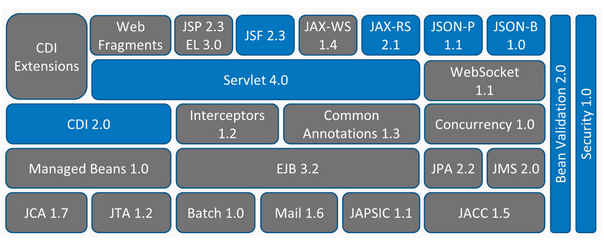
\includegraphics[width=0.6\textwidth]{imaxes/JakartaEE-Architecture.png}
  \caption{Arquitectura Jakarta EE}
  \label{fig:arquitecturaJakartaEE}
\end{figure}

Entre las distintas especificaciones de \acrshort{jee} cabe destacar las siguientes:
\begin{itemize}
   \item Especificaciones web
     \begin{itemize}
       \item Jakarta Servlet: define cómo gestionar las solicitudes \acrfull{http}, de forma síncrona o asíncrona. Es de bajo nivel y otras especificaciones de \acrshort{jee} dependen de él.
	   \item Jakarta WebSocket: define un conjunto de \acrshort{api} para dar servicio a las conexiones de WebSocket
   	   \item \acrshort{jsf} (\acrlong{jsf}): una tecnología para construir interfaces de usuario a partir de componentes.
  	   \item Jakarta \acrshort{el} (\acrlong{el}) es un lenguaje simple diseñado originalmente para satisfacer las necesidades específicas de los desarrolladores de aplicaciones web.
     \end{itemize} 
   \item Especificaciones de servicios web
     \begin{itemize}
       \item Jakarta RESTful Web Services: proporciona soporte en la creación de servicios web de acuerdo con el patrón arquitectónico de \acrfull{rest}.
  	   \item Jakarta JSON Processing: conjunto de especificaciones para gestionar la información codificada en formato \acrfull{json}.
	   \item Jakarta JSON Binding: proporciona especificaciones para convertir información \acrshort{json}. en o desde clases Java
 	   \item Jakarta XML Binding: permite asignar \acrfull{xml} a objetos Java; Los servicios Web \acrshort{xml} de Jakarta se pueden utilizar para crear servicios web \acrfull{soap}.
     \end{itemize}
     
   \item Especificaciones empresariales
     \begin{itemize}
        \item Jakarta Activation (JAF): especifica una arquitectura para extender los beans de componentes proporcionando tipos de datos y enlaces de dichos tipos. 
        \item Jakarta \acrshort{cdi} (\acrlong{cdi}): es una especificación para proporcionar un contenedor de inyección de dependencias
        \item \acrshort{ejb} (\acrlong{ejb}) define un conjunto de \acrshort{api} ligeras que un contenedor de objetos (el contenedor \acrshort{ejb}) admitirá para proporcionar transacciones, llamadas a procedimientos remotos, control de simultaneidad, inyección de dependencias y control de acceso para objetos de negocio. Este paquete contiene las clases e interfaces de \acrshort{ejb} que definen los contratos entre el bean empresarial y sus clientes y entre el bean empresarial y el contenedor ejb. 
        \item \acrshort{jpa} (\acrlong{jpa}): especificaciones sobre el mapeo objeto-relacional entre tablas de bases de datos de relaciones y clases Java.
        \item \acrshort{jta} (\acrlong{jta}): contiene las interfaces y anotaciones para interactuar con el soporte de transacciones ofrecido por Jakarta EE.
	    \item \acrshort{jms} (\acrlong{jms}) proporciona una forma común para que los programas Java creen, envíen, reciban y lean los mensajes de un sistema de mensajería empresarial.      
     \end{itemize}
     
   \item Otras especificaciones
     \begin{itemize}
        \item Validación: contiene las anotaciones e interfaces para el soporte de validación declarativa ofrecido por la \acrshort{api} de validación de Bean. 
		\item Jakarta Batch: proporciona los medios para que el procesamiento por lotes en aplicaciones ejecute tareas en segundo plano de larga duración que posiblemente impliquen un gran volumen de datos y que puedan necesitar ser ejecutadas periódicamente. 
		\item Jakarta Connectors: herramienta basada en Java para conectar servidores de aplicaciones y \acrfull{eis} como parte de la integración de \acrfull{eai}. Esta es una \acrshort{api} de bajo nivel dirigida a proveedores con los que el desarrollador de aplicaciones promedio generalmente no entra en contacto.
     \end{itemize}
\end{itemize}




\subsection{Componentes Jakarta EE}
\label{sec:componentes}
\acrshort{jee} define cuatro tipos de componentes de aplicación~\cite{JakartaEE}:
\begin{itemize}
   \item Aplicaciones cliente: suelen ser programas \acrfull{gui} que se ejecutan en un equipo de escritorio.
   \item Applets: son componentes de \acrshort{gui} que normalmente se ejecutan en un navegador web, pero pueden ejecutarse en una variedad de otras aplicaciones o dispositivos que admiten el modelo de programación de applets. 
   \item Aplicaciones web como servlets, páginas \acrfull{jsp} y \acrshort{jsf} que se ejecutan en un contenedor web y responden a las peticiones \acrshort{http} del cliente.
   \item Aplicaciones empresariales como los componentes \acrshort{ejb}, \acrshort{jta} o \acrshort{jms}, que se ejecutan en un contenedor \acrshort{ejb} .
\end{itemize}



\subsection{Contenedores}
\label{sec:contenedores}
\acrshort{jee} se divide en dominios lógicos llamados contenedores. En una aplicación \acrshort{jee} los componentes nunca interactúan con otros componentes de la aplicación si no que utilizan los protocolos y métodos del contenedor para interactuar entre sí y con los servicios de la plataforma~\cite{JakartaEE}. Cada contenedor tiene una función específica, soporta un conjunto de \acrshort{api} y ofrece servicios a los componentes tales como seguridad, acceso a base de datos, gestión de transacciones, nombres de directorios e inyección de recursos. Los contenedores ocultan la complejidad técnica y mejoran la portabilidad lo que permite al desarrollador centrarse en la lógica de aplicación en lugar de resolver problemas técnicos. Por ejemplo el contenedor \acrshort{ejb} es responsable de administrar la ejecución de los beans que contienen la lógica de negocio.

\subsubsection{Servidores}
\label{sec:servidores}
Detrás de un contenedor \acrshort{jee} se encuentra el servidor del que forma parte~\cite{JakartaEE}. Un proveedor de productos de \acrshort{jee}  por lo general implementa la funcionalidad del lado del servidor de \acrshort{jee}  usando una infraestructura de transacciones existente en combinación con la tecnología \acrshort{jse} de la plataforma Java. La funcionalidad del cliente \acrshort{jee} se basa por lo general en la tecnología \acrshort{jse} .




\section{Librerías y componentes Jakarta EE usados}
\label{sec:componentesJakartaEE}

A continuación ofrecemos una relación de las principales librerías y componentes \acrshort{jee} usados en el desarrollo de este \acrshort{tfg}.

\subsection{Jakarta Enterprise Bean}
\label{sec:jeb}

Un \acrfull{ejb} es un componente del lado del servidor que encapsula la lógica empresarial de una aplicación. La lógica de negocio es el código que cumple el propósito de la aplicación~\cite{JEE7-Tutorial}.

Estos componentes se ejecutan en el contenedor \acrshort{ejb}. Aunque es transparente para el desarrollador de aplicaciones, el contenedor \acrshort{ejb} proporciona servicios a nivel de sistema tales como transacciones y seguridad a sus enterprise beans. Estos servicios le permiten crear e implementar rápidamente \acrshort{ejb}, que son los que forman el núcleo de las aplicaciones transaccionales de \acrshort{jee}.

Entre las ventajas que ofrecen los \textit{enterprise beans} se encuentran los siguientes:
\begin{itemize}
\item Simplifican el desarrollo de la aplicación ya que es el contenedor \acrshort{ejb} el que se encarga de gestionar los servicios a nivel de sistema, como la gestión de transacciones y la autorización de seguridad.
\item La lógica del negocio reside en los \textit{enterprise beans} y no en el lado del cliente, permitiendo que el desarrollo del lado del cliente este desacoplado de la lógica del negocio.
\item Los \textit{enterprise beans} son componentes portables, reutilizables y pueden ser desplegados en servidores que usen los estándares del  \acrshort{jee} \acrshort{jee}.
\item Pueden residir en diferentes servidores pudiendo ser invocados por un cliente remoto.
\end{itemize}

El uso \textit{enterprise beans} está recomendado en aplicaciones escalables, en aquellas en las que necesitemos asegurar la integridad de los datos y/o en aplicaciones con variedad de clientes.


\subsection{Java Server Faces}
\label{sec:jsf}
\acrfull{jsf} es una tecnología para el desarrollo de \acrshort{gui} en aplicaciones web dentro de la plataforma \acrshort{jee}~\cite{DesarrolloJakartaEE}.

La especificación está definida por \acrfull{jcp}, lo que lo convierte en un estándar. Se basa en la utilización del patrón  \acrfull{mvc} que tiene como objetivo separar los datos (modelo) de su procesamiento (controlador) y la forma en la que estos son presentados al usuario en una aplicación (vista).\acrshort{jsf} oculta al programador los detalles de las peticiones y respuestas \acrshort{http}, simplificando la programación de aplicaciones web y acercándolas a un estilo de desarrollo similar al de las aplicaciones de escritorio.

En \acrshort{jsf} se define un \emph{servlet} llamado \emph{\textbf{Faces Servlet}} dentro de un archivo de configuración llamado \emph{web.xml}, que tiene como objetivo recibir las distintas solicitudes \acrshort{http} de los cliente y procesarlas. 

\subsubsection{Ciclo de vida de una aplicación JSF}
\label{sec:ciclo-vida-jsf}
El ciclo de vida de una aplicación \acrshort{jsf} consta de las siguientes fases~\cite{DesarrolloJakartaEE}:
\begin{enumerate}
\item Restaurar la vista: en esta etapa \acrshort{jsf} comprueba si la solicitud \acrshort{http} recibida es nueva o no con el fin de crear o restaurar el árbol de componentes (objetos Java necesarios).
\item Aplicar los valores de la solicitud: una vez creado el árbol cada componente actualiza sus valores con los parámetros presentes en la solicitud.
\item Procesar validaciones: valida y convierte los datos que el usuario ingresó al tipo que corresponda. En caso de que se produzca algún error, se saltará a la etapa de renderización, en la que se le informará al usuario de los errores producidos. En caso contrario se pasará a la siguiente fase (actualizar valores).
\item Actualizar los valores del modelo: se refresca el árbol de componentes actualizando los valores del modelo.
\item Invocar la lógica de la aplicación: se invocan los métodos solicitados por el usuario.
\item Renderizar la respuesta: se envía al cliente la respuesta en \acrshort{html}.
\end{enumerate}


\subsection{Primefaces}
\label{sec:primefaces}

Primefaces es un \emph{framework} de \gls{opensource} para \acrshort{jsf} que cuenta con un amplio conjunto de componentes enriquecidos para diseñar interfaces de usuario creada por PrimeTek Informatics. El desarrollo inicial de PrimeFaces se inició a finales de 2008.

Las principales características que presenta son las siguientes~\cite{Primefaces}:
\begin{itemize}
\item Amplio conjunto de componentes (HtmlEditor, Dialog, Autocompletar, Gráficos y muchos más).
\item Soporte nativo AJAX basado en API JSF AJAX estándar. 
\item Ligero, sin necesidad de dependencias ni configuraciones adicionales. 
\item Capacidad de respuesta y accesibilidad incorporadas. 
\item Amplia documentación y comunidad de usuarios.
\end{itemize}


\subsection{Omnifaces}
\label{sec:omnifaces}

OmniFaces es una biblioteca de utilidades open source para \acrshort{jsf} desarrollada por dos miembros de la JSF Expert Group (JSF EG), Bauke Scholtz (alias BalusC) y Arjan Tijms.

A diferencia de otras bibliotecas de componentes \acrshort{jsf}  existentes en el mercado (como PrimeFaces, BootsFaces o ButterFaces), OmniFaces no contiene ningún componente orientado a embellecer la visualización, si no que está más orientado a las \textit{utilidades} que resuelven problemas prácticos cotidianos y soluciones para (pequeñas) deficiencias en la \acrshort{api}  \acrshort{jsf}. Esta librería se centra en utilidades que facilitan las tareas cotidianas con la \acrshort{api} \acrshort{jsf} estándar. Estamos ante una respuesta a los problemas recurrentes con los que los autores se han encontrado a lo largo de su desarrollo profesional con \acrshort{jsf} y de las preguntas que se publican en Stack Overflow.

\subsection{Java Object Orientated Query}
\label{sec:jooq}
\acrfull{jooq} es una biblioteca de software de asignación de bases de datos ligera en Java que implementa el patrón de registro activo desarrollada por Lukas Eder. Su propósito es ser tanto relacional como orientado a objetos al proporcionar por un lado un lenguaje específico del dominio para construir consultas SQL seguras y por otro generar clases a partir de un esquema de base de datos a través de su \acrshort{api} fluida sobre las que construir dichas consultas.

El enfoque de \acrshort{jooq} pone el foco en el lado de \acrfull{sql} en lugar de \acrshort{jpa} como hacen los \acrfull{orm} como por ejemplo Hibernate.

Alguna de las características que presenta \acrshort{jooq} son las siguientes\citep{VentajasJooq}:
\begin{itemize}
\item Proporciona un generador de código que permite, mediante ingeniería inversa, convertir el esquema de base de datos en conjunto de tablas de modelado de clases Java, registros, secuencias, POJO, DAO, procedimientos almacenados, tipos definidos por el usuario y muchos más listas para usarse. 
\item Ofrece la posibilidad de utilizar toda la funcionalidad de la base de datos seleccionada en lugar de una abstracción o un subconjunto limitado gracias a su \acrfull{dsl} fluido que se asigna uno a uno con \acrshort{sql}
\item El \acrfull{dsl} que genera permite que su IDE se complete automáticamente mientras escribe las consultas.
\item Utiliza el sistema de tipos de Java para garantizar que el SQL que genera es válido.
\item La \acrshort{api} de \acrshort{jooq} hace todo lo posible para asegurarse de que está utilizando el tipo de datos Java correcto para cada columna de su base de datos. 
\item Presenta una extensión de conversor de tipos fácil de usar para transformar tipos de datos comunes, como Timestamp o \acrshort{sql} Date/Time a java.time.ZonedDateTime.
\item Existe una funcionalidad de mapeo que ayuda a asignar conjuntos de resultados a \acrfull{pojo} y proporciona una implementación del patrón de registro activo para trabajar de una manera similar a \acrshort{orm}
\item Se pueden usar los streams existentes a partir de Java 8 para transformar conjuntos de resultados de forma fácil y sucinta.
\item Si se producen cambios en el esquema de la base de datos se obtienen errores de compilación en lugar de los de tiempo de ejecución.
\item Funciona con las principales bases de datos relacionales: MS Access, MS Access 2013, CUBRID, IBM DB2, Apache Derby, Firebird, H2, Hypersonic, Informix, Ingres, MariaDB, MySQL, Oracle, Oracle, PostgreSQL, SQLite, SQL Server, SQL Server y Sybase.
\item Tiene doble licencia, siendo de uso gratuito para todas las bases de datos de código abierto.
\end{itemize}

\subsection{Log4j}
 Es una biblioteca \gls{opensource} perteneciente a los Java Logging Frameworks desarrollada en Java por la Apache Software Foundation que permite generar mensajes de logging de una forma limpia, sencilla, permitiendo filtrarlos por importancia y pudiendo configurar su salida por vía consola, fichero u otras distintas.

Existen diversos niveles de prioridad. A continuación se muestran los más utilizados
\begin{itemize}
\item DEBUG: usado para escribir mensajes de depuración.
\item INFO: mensajes puramente informativos.
\item WARN: alertas. Generalmente utilizados para alertar de eventos de los que se quiere dejar constancia pero que no afectan al correcto funcionamiento de la aplicación.
\item ERROR: usado para mensajes de eventos que afectan al programa pero lo dejan seguir funcionando (por ejemplo un parámetro figura como vacío por lo que se se carga el parámetro por defecto).
\item FATAL: usado para errores críticos. 
\end{itemize}  
  
    


\section{Formatos de almacenamiento. PostgreSQL}
\label{sec:almacenamiento}

Los datos se han almacenado en una base de datos relacional. Para ello se ha optado por el gestor de base de datos de código abierto PostgreSQL, ya que se trata de una solución robusta, con amplias funcionalidades cuyo uso está cada vez más extendido y es 100\% open source~\cite{Postgresql}.


\subsection{Historia}
\label{sec:historiapsql}

El sistema de gestión de bases de datos objeto-relacionales ahora conocido como PostgreSQL se deriva del paquete POSTGRES escrito en la Universidad de California en Berkeley.

\paragraph{Inicios}
La implementación de POSTGRES comenzó en 1986. Desde entonces ha tenido varios lanzamientos importantes. El primer sistema \emph{``demoware''}\footnote{Tipo de software que permite su uso sin ninguna restricción por un período limitado de tiempo, por un número de usos o por progresión hasta un determinado punto. Generalmente pasado el período de prueba, se deshabilitan todas las funciones o parte de ellas.} entró en funcionamiento en 1987 y se mostró en la Conferencia ACM-SIGMOD de 1988. La versión 1 fue lanzada a algunos usuarios externos en junio de 1989. La Versión 2 fue lanzada en junio de 1990 con un nuevo sistema de reglas. La versión 3 apareció en 1991 y agregó soporte para múltiples administradores de almacenamiento, un ejecutor de consultas mejorado y un sistema de reglas reescrito. En su mayor parte, las versiones posteriores hasta Postgres95 se centraron en la portabilidad y la confiabilidad.

POSTGRES se ha utilizado para implementar muchas aplicaciones diferentes de investigación y producción. También se ha utilizado como una herramienta educativa en varias universidades. A finales de 1992, POSTGRES se convirtió en el principal gestor de datos del proyecto de computación científica Sequoia 2000.

\paragraph{Postgres95}
En 1994, Andrew Yu y Jolly Chen agregaron un intérprete de lenguaje \acrshort{sql} a POSTGRES. Bajo un nuevo nombre, Postgres95 fue posteriormente lanzado a la web para encontrar su propio camino en el mundo como un descendiente de código abierto del código original de POSTGRES Berkeley. Estaba codificado completamente en ANSI C y redujo su tamaño un 25\% respecto al código original. También se mejoró el rendimiento y la capacidad de mantenimiento.

\paragraph{PostgreSQL}
En 1996 se eligió un nuevo nombre, PostgreSQL, para reflejar la relación entre el POSTGRES original y las versiones más recientes con capacidad \acrshort{sql}. Al mismo tiempo se configuró la numeración de la versión para que comenzara en 6.0, poniendo los números de nuevo en la secuencia originalmente iniciada por el proyecto POSTGRES de Berkeley.

Durante el desarrollo de PostgreSQL el foco se trasladó hacia el aumento de las características y capacidades .

\subsection{Características}
\label{sec:caracteristicas}

PostgreSQL es compatible con una gran parte del estándar SQL y entre sus características figuran las siguientes: 
\begin{itemize}
\item Es \textit{open source}.
\item Emplea un lenguaje SQL estándar lo que permite la importación de otras bases de datos.
\item Cumple con el modelo ACID (atomicidad, consistencia, aislamiento y durabilidad de los datos almacenados).
\item Capacidad de realizar consultas complejas.
\item Claves foráneas.
\item Triggers (disparadores).
\item Vistas actualizables.
\item Integridad transaccional.
\item Control de versiones simultánea.
\end{itemize}

También permite ampliaciones por parte del usuario de múltiples formas, por ejemplo mediante la agregación de:
\begin{itemize}
\item Nuevos tipos de datos 
\item Funciones 
\item Operadores 
\item Funciones agregadas 
\item Lenguajes procedurales 
\item Extensiones
\end{itemize}



 \chapter{Metodología}
\label{chap:metodologia}

\lettrine{E} {n} informática se define la metodología como \textquote{un proceso para producir software de forma organizada, empleando una colección de técnicas y convenciones de notación predefinidas.}

Existen distintas metodologías de desarrollo de software. Para desarrolla este \acrshort{tfg} nos hemos basado en una metodología clásica basada en el método incremental, ya que se partía de una báse de conocimiento del proceso de negocio previa pero no así de la tecnología a usar.

Nuestro modelo incremental ha constado de tres fases, cada una de las cuales ha contado con sus correspondiente parte de análisis, diseño, codificación y pruebas y ha culminado con una entrega del producto completamente operacional atendiendo a los requisitos especificados para dicha fase.

\section{Descripción de las fases definidas}
\label{sec:metodologia-fases}

A continuación se muestra una breve descripción para cada una de las fases definidas con el método incremental usado. Los casos de uso definidos en cada una de las fases se detallan en el anexo \ref{chap:ref-tecnica}.

\subsection{Fase I - Fase inicial}
Finalización estimada de la fase: finales de mayo.

En esta fase se realiza un análisis global del producto a desarrollar, realizando una primera aproximación a los elementos que deberá contener.
Se realiza un análisis de los requistos técnicos necesarios para llevar a cabo el desarrollo y se establece el entorno de desarrollo, realizando las instalaciones y configuraciones pertinentes. 

Atendiendo a la parte funcional del producto a desarrollar, esta fase se centra en crear la estructura del proyecto: el acceso a la aplicación y la parte correspondiente a los elementos de parametrización y de catálogo simple, los elementos con menor complejidad de la aplicación. Se realiza la parte de análisis, diseño, codificación y pruebas correspondientes a los casos de uso \textbf{CU-02 Inicio de sesión}, \textbf{CU-02 Fin de sesión}, \textbf{CU-19 Gestionar ficha personal}, \textbf{CU-29 Gestión de usuarios}, \textbf{CU-22 Acceder parametrización}, \textbf{CU-23 Acceder catálogo entidad simple} y \textbf{CU-25 Acceder a relacion simple del catálogo}, (con sus correspondientes casos de uso anidados). 


\subsection{Fase II - Elementos históricos}
Finalización estimada de la fase: mediados de julio.

Esta fase se centra en el desarrollo de las entidades con histórico del catálogo. Se realiza la parte de análisis, diseño, codificación y pruebas correspondientes a los casos de uso \textbf{CU-24 Acceder al catálogo entidad con históricos} y \textbf{CU-26 Acceder a relacion con histórico del catálogo} (con sus correspondientes casos de uso anidados).


\subsection{Fase III - Contratación}
Finalización estimada de la fase: finales de agosto.

Fase final del proyecto que se centra en el desarrollo de las instancias del catálogo y la vista jerárquica de la contratación. Se realiza la parte de análisis, diseño, codificación y pruebas correspondientes a los casos de uso \textbf{CU-26 Acceder a relacion con histórico del catálogo} y \textbf{CU-28 Acceder jerarquía} (con sus correspondientes casos de uso anidados). 



 
 \chapter{Análisis y diseño}
\label{chap:analisis-diseño}


\lettrine{E}{n} este capítulo nos centraremos en el análisis y posterior diseño realizado en este \acrshort{tfg} para el desarrollo de la herramienta de gestión de contratación propuesta.

\section{Análisis de las necesidades}
\label{sec:analisis}
Se pretende desarrollar una aplicación web de \gls{opensource} que permita registrar las distintas contrataciones realizadas por los clientes de una empresa proveedora de servicios. Puesto que las contrataciones se realizan sobre el catálogo de servicios de la empresa, también proveerá de las herramientas necesarias para mantener dicho catálogo. Asimismo deberá permitir definir una serie de elementos parmetrizables necesarios para definir las distintas entidades que alberga dicha aplicación. Por lo tanto las entidades a tratar en el sistema se englobarán en tres grandes grupos:
\begin{itemize}
\item Parametrización: esta categoría engloba todos los elementos de parametrización necesarios para la definición de las distintas entidades del sistema (niveles de aplicación, tipos de descuento, tipos impositivos, etc.).
\item Catálogo: esta categoría engloba todos los elementos que definen el catálogo de servicios de la empresa (tipos de productos, servicios, cuotas, etc. y sus relaciones), así como los tipos de entidades que definen el catálogo de clientes y contrataciones (tipos de clientes, tipos de ciclos de facturación, etc.).
\item Instancia: esta categoría engloba todos los elementos que conforman las contrataciones: clientes, cuentas, elementos contratados, etc.
\end{itemize}


La aplicación de gestión de la contratación propuesta será utilizada, principalmente, por el personal del departamento de contratación y ventas de una empresa, que podrá llevar a cabo las pertinentes altas, bajas y modificaciones; pero también por personal de otros departamentos que pueda necesitar acceder puntualmente a información recogida en la herramienta con el fin de poder llevar a cabo sus tareas. Estos usuarios pertenecientes a otros departamentes han de tener limitado el acceso a ciertas funcionalidades definidas en la aplicación. Además existirá una figura de administrador, que tendrá acceso a funcionalidades avanzadas.


Es por ello que se definen tres perfiles de acceso a la herramienta en función de las funcionalidades a las que se le quiera dar acceso al usuario. Dichos perfiles serán los siguientes:
\begin{itemize}
\item READ: perfil que da sólo acceso a la consulta de los datos almacenados en el sistema, esto es, los usuarios que tengan este perfil asociado solo podrán listar la información, pero no podrán realizar ninguna modificación sobre los mismos.
\item MODIF: perfil que además de permitir la consulta de los datos almacenados en el sistema permite realizar altas, bajas y modificaciones sobre todos los elementos que conforman el sistema.
\item ADMIN: perfil que amplía el acceso a las funcionalidades definidas para el perfil MODIF, otorgándole acceso a la gestión de usuarios: podrá dar de alta nuevos usuarios, modificar usuarios existentes (incluido el cambio de contraseña) o darlos de baja.
\end{itemize}


Con el fin de poder hacer un seguimiento de los distintos cambios producidos en el sistema se deberá llevar registro de la creación de los elementos  del catálogo y de las instancias, así como de la última modificación realizada.

También con el objetivo de poder llevar un registro sobre los cambios producidos sobre determinadas entidades que pueden sufrir cambios durante su ciclo de vida se establecen registros de histórico para dichas entidades. El objetivo de estos históricos es poder tener la \textit{foto} del estado de una determinada entidad en un momento determinado, por ejemplo, el precio que tenía la definición de una cuota determinada o los distintos servicios activos de un cliente en una fecha determinada.


Esta aplicación tendrá el objetivo de formar parte de un ecosistema mayor, integrándose en una segunda fase con el resto de herramientas de la empresa para conformar el área comercial de la misma. En la \figurename~\ref{fig:area-comercial} se muestra un esquema con las distintas aplicaciones que típicamente darían soporte a la actividad comercial de una empresa de servicios TIC. El flujo de contratación en un sistema integrado sería el siguiente y sería análogo para el caso de modificaciones o bajas de contrataciones:
\begin{enumerate}
\item Se registra una contratación en el sistema de contrataciones. Éste notifica al sistema de provisiones la contratación y queda a la espera de que le confirmen que todos los servicios están provisionados. 
\item Una vez provisionados, el sistema de provisión notificará al sistema de contratación del fin de la provión y éste facilita al sistema facturador todos los elementos necesarios para registrar esa contratacion en el sistema y realizar las correspondientes facturaciones. 
\item En caso de que se produzca algún cambio de estado de alguna de las entidades contratadas por parte del sistema de facturación, éste notificará del cambio al sistema de contrataciones. Estos cambios pueden obdecer a impagos incurridos por el cliente, los cuales son notificados al facturador por el sistema de cobros (a quien el facturado envía los recibos de las facturas generadas para su puesta a cobro).
\end{enumerate}

La relación que se muestra entre el sistema de facturación y el de tarificación se refiere a los consumos que pueden realizar las distintas entidades facturables contratadas (el sistema de facturación notifica al de tarificación las nuevas entidades dadas de alta, modificadas o dadas de baja susceptibles de generar consumos , y el sistema de tarificación le envía al sistema de facturación los datos de los consumos realizados en tiempo real para su facturación).


\begin{figure}
  \centering
  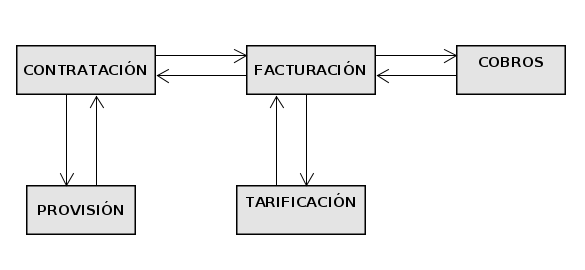
\includegraphics[width=0.55\textwidth]{imaxes/area-comercial.png}
  \caption{Entorno comercial y la comunicación establecida entre las distintas áreas de negocio.}
  \label{fig:area-comercial}
\end{figure}


\subsection{Catálogo de servicios}
\label{sub:catalogo-chap-analisis}

\acrshort{itil} define el catálogo de servicios como~\cite{catalogoITIL}:
\textquote{una base de datos centralizada que contiene información precisa sobre las ofertas de servicios de TI activas y un subconjunto de la cartera de servicios del proveedor de servicios de TI}. De forma simple vendría siendo la \textit{mercancía} que ofrece una determinada empresa. Pero va un paso más allá del mero listado de elementos ofertados en este momento, pues lleva además el registro del ciclo de vida de todos los productos y servicios gestionados por la empresa, tanto los servicios y productos retirados como los que se ofrecen actualmente e incluso los que están en desarrollo.

Entendemos por prestación de servicios aquella actividad o actividades llevadas a cabo por un proveedor con el propósito de satisfacer una determinada necesidad del cliente a través de servicios, entendiendo por servicio un activo de naturaleza económica intangible.

La idea es la siguiente: la empresa define su catálogo de servicios (tecnología a ofertar), los elementos facturables a aplicar por la prestación de servicios y los descuentos existentes sobre dichos elementos facturables. Se distinguen dos tipos de elementos facturables: cuotas (cargos periódicos asociados a la prestación de los distintos servicios) y consumos (cargos puntuales derivados del consumo de algún elemento definido como consumible).
El catálogo de servicios de nuestra empresa estará formado por cinco entidades principales y las relaciones que guardan entre sí. Dichas entidades son las siguientes:

\paragraph{Tipo de producto.} Es el elemento raíz del catálogo del sistema sobre el que se irán definiendo el resto de elementos que se pueden ofrecer al cliente. Podemos verlo como el \textit{paquete} que contendrá todo lo que se le ofrece al cliente.
\paragraph{Tipo de servicio.} Es el elemento que realmente aporta valor al cliente, ya que es el que define el elemento que va a aportar el valor de la contratación, por ejemplo la línea de telefono.
\paragraph{Tipo de promoción.} Es el elemento que definen los descuentos que ofrece la empresa. Su ámbito de aplicación se circunscribe a productos y servicios y forma parte de su definición. El descuento se aplicará sobre los distintos elementos facturables existente en el sistema.
\paragraph{Tipo de cuota.} Es el elemento que define la contraprestación económica que va a recibir la empresa de forma periódica por la prestación de servicios que ofrece al cliente. Su ámbito de aplicación se circunscribe a productos y servicios y forma parte de la definición del tipo de producto o servicio.
\paragraph{Tipo de consumos.} Es el elemento que define el consumo puntual de un determinado elemento por parte del cliente, como puede ser una llamada de teléfono. Sólo tiene interés desde el punto de vista de la definición de la aplicación de los distintos descuentos, ya que a diferencia de las cuotas, para las que podemos definir un precio cerrado que puede conocerse de antemano, el importe de los consumos vendrá definido por la naturaleza propia del evento del consumo (por ejemplo, el coste de una llamada de teléfono viene dado, además de por el tipo de llamada, que lleva asociado un precio por minuto, por la duración de la misma o la franja horaria en la que se realiza) por lo que en la herramienta simplemente se definirán los consumos susceptibles de ser descontados. Se considera un único ámbito de aplicación: el de servicio.

Y las relaciones que se establecen entre ellas como se muestra en el diagrama de la \figurename~\ref{fig:catalogo-chap-analisis}) y son como sigue:

\begin{itemize}
\item Un tipo de producto consta de:
	\begin{itemize}
		\item Uno o más tipos de servicio.
		\item Cero, uno o más tipos de cuotas.
		\item Cero, uno o más tipos de promociones.
	\end{itemize}
\item Un servicio consta de:
	\begin{itemize}
		\item Cero, uno o más tipos de cuotas.
		\item Cero, uno o más tipos de promociones.
	\end{itemize}
		\item Un tipo de cuota puede estar relacionada con 
	\begin{itemize}
		\item Cero, uno o más tipos de productos.
		\item Cero, uno o más tipos de servicios.
		\item Cero, uno o más tipos de promociones.
	\end{itemize}
\item Un tipo de promoción puede estar relacionada con 
	\begin{itemize}
		\item Cero, uno o más tipos de productos.
		\item Cero, uno o más tipos de servicios.
		\item Uno o más tipos de cuotas.
		\item Uno o más tipos de consumos.
	\end{itemize}
\end{itemize}


\begin{figure}
  \centering
  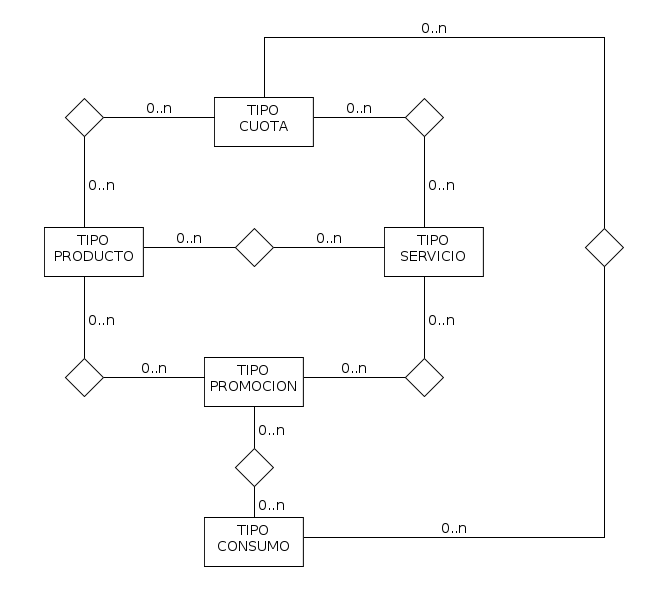
\includegraphics[width=0.55\textwidth]{imaxes/catalogo.png}
  \caption{Modelo Entidad-Relación del catálogo de servicios.}
  \label{fig:catalogo-chap-analisis}
\end{figure}

\paragraph{}
Puesto que el catálogo de servicios contiene la definición de los distintos elementos que podrán contratarse, hemos incluido dentro del concepto de catálogo otros elementos que permiten definir la plantilla con la que crear la posterior \textit{instanciación} de las mismas, a saber:

\paragraph{Tipo de ciclo de facturación.} La instanciación de los distintos ciclos de facturación no forma parte del ámbito de la herramienta de contratación propiamente (entraría dentro del ámbito de facturación) pero puesto que forma parte de la definición de los distintos tipos de cuentas existentes, incluimos la definición del tipo de ciclo de facturación en la herramienta a desarrollar.

\paragraph{Tipo de cliente.} Esta entidad permitirá la creación de clientes atendiendo a una clasificación definida por la empresa, por ejemplo para distinguir entre clientes particulares de clientes de empresa.

\paragraph{Tipo de cuenta.} La cuenta es la entidad sobre la que se realizarán las contrataciones, que a su vez dependerá de un cliente particular. La cuenta estará definida por una serie de valores especificados en la tipología de la misma, como el tipo de pago.



\subsection{Contratación}
\label{sub:contratacion-chap-analisis}
La contratación contendrá la implementación (instancia) real de los distintos elementos definidos en el catálogo, esto es el conjunto de clientes y sus relaciones con los productos y servicios contratados. La \figurename~\ref{fig:contratacion-chap-analisis} muestra el diagrama de clases para la gestión de la contratación.



\begin{figure}
  \centering
  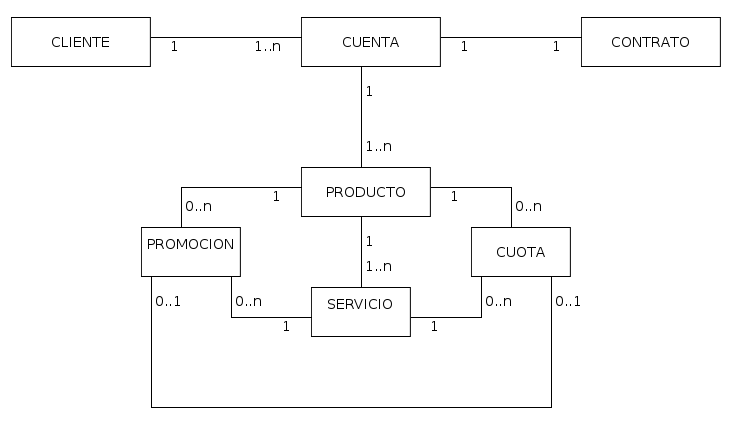
\includegraphics[width=0.55\textwidth]{imaxes/instancia.png}
  \caption{Modelo de Contratación}
  \label{fig:contratacion-chap-analisis}
\end{figure}


\subsection{Elementos de parametrización}
\label{sub:parametrizacion-chap-analisis}
Los elementos de parametrización son elementos que nos permiten modelar entidades superiores para que se comporten de una forma determinada. No es lo mismo aplicar un descuento en forma de porcentaje sobre el total que en número de unidades contratadas. Para el desarrollo de la herramienta se han considerado los siguientes elementos de parametrización.
\begin{description}
\item[Endidades:] define los distintos tipos de entidades definidas en el sistema.
\item[Clases de consumo:] define las distintas clases de consumo definidas en el sistema (llamadas a fijo, a móviles, sms,\dots).
\item[Estado:] para reflejar los distintos estados que tienen las entidades del sistema a lo largo de su ciclo de vida.
\item[Nivel de aplicación:] para indicar sobre qué entidad aplican las distintas cuotas y promociones: si sobre un producto o sobre un servicio.
\item[Tipos de descuento:] reflejan los distintos tipos de descuento que pueden tenerse en cuenta (porcentaje sobre el total, unidades de consumo,\dots).
\item[Tipos de pago:] reflejan los distintos métodos de pago que contempla la empresa (domiciliación bancaria, transferencia,\dots).
\item[Período de facturación:] define el número de días que conforman los  períodos de facturación.
\item[Tipo impositivo:] define los distintos tipos impositivos que contempla la aplicación (iva, igic,\dots) y sus valores porcentuales de aplicación.
\item[Tipo de documento de identificación:] define los distintos tipos de documento de identificación contemplados por el sistema.
\end{description}




\section{Casos de uso}
\label{sec:casos-uso-chap-analisis}

Se consideran tres tipos de usuarios de la aplicación en función de los funcionalidades que puedan realizar en la misma en función del perfil que tengan asignado. Los perfiles definidos para la aplicación son los siguientes:
\begin{itemize}
\item READ: perfil de sólo lectura. Solamente permite visualizar la información almacenada en la aplicación, pero no puede realizar ninguna modificación, salvo la relativa a su información de contacto y su contraseña.
\item MODIF: perfil de lectura y modificación. Además de las funcionalidades descritas para el perfil READ, permite realizar modificaciones sobre las distintas entidades del sistema (altas/bajas/modificaciones).
\item ADMIN: perfil de administrador. Además de las funcionalidades descritas para el perfil WRITE, permite la gestión de usuarios (altas/bajas/modificaciones).
\end{itemize}


\subsection{Actores}
\label{sub:actores-chap-analisis}

El actor ADMIN representa a los usuarios de la aplicación que tienen
acceso completo a todas las funciones, incluyendo la gestión de usuarios.

Los actores  READ y  WRITE representan a cualquier usuario con un perfil READ o MODIF, respectivamente, que haya sido dado de alta previamente por un actor ADMIN, que representa a cualquier usuario con perfil ADMIN, y disponga de un nombre de usuario y una contraseña.


\subsection{Casos de uso}
\label{sub:casos-uso-chap-analisis}


Todos los usuarios comparten los casos de uso de acceso y los relativos a la consulta de las entidades del sistema. El actor WRITE amplía esos casos de uso con funcionalidades de creación, modificación y borrado de entidades y por último el actor ADMIN amplía esos casos de uso con el caso de uso de administración de usuarios. Las siguientes figuras (\figurename{}s~\ref{fig:cu-acceso-chap-analisis}, \ref{fig:cu-read-write-chap-analisis} y \ref{fig:cu-admin-chap-analisis}) muestran una visión de alto nivel de los distintos casos de uso definidos en el sistema. Dichos casos de uso se analizan con más detalle en los siguientes apartados.


\begin{figure}[H]
  \centering
  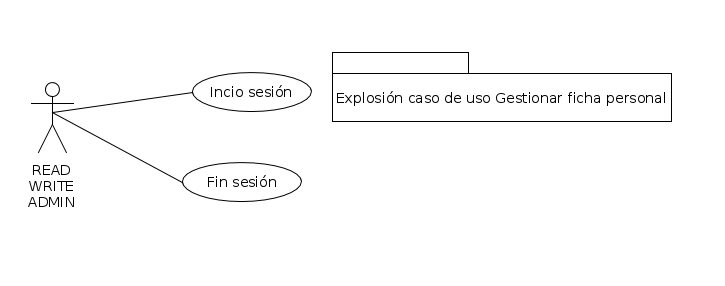
\includegraphics[width=0.6\textwidth]{imaxes/cu_acceso.png}
  \caption{Caso de uso del acceso al sistema - Actores READ, WRITE y ADMIN}
  \label{fig:cu-acceso-chap-analisis}
\end{figure}



\begin{figure}[H]
  \centering
  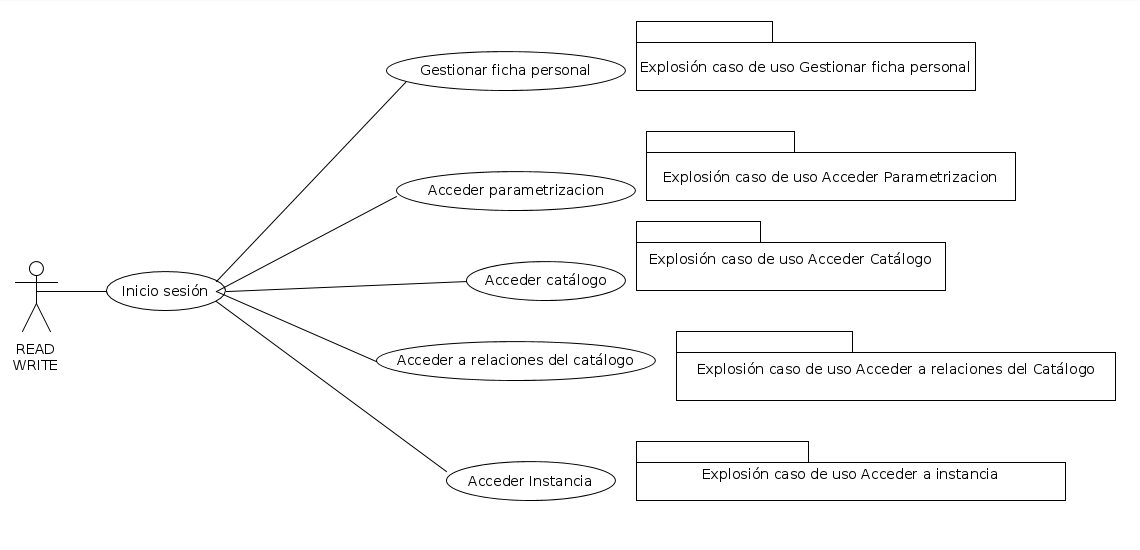
\includegraphics[width=\textwidth]{imaxes/cu-read-write.png}
  \caption{Casos de uso de los actores READ, WRITE}
  \label{fig:cu-read-write-chap-analisis}
\end{figure}


\begin{figure}[H]
  \centering
  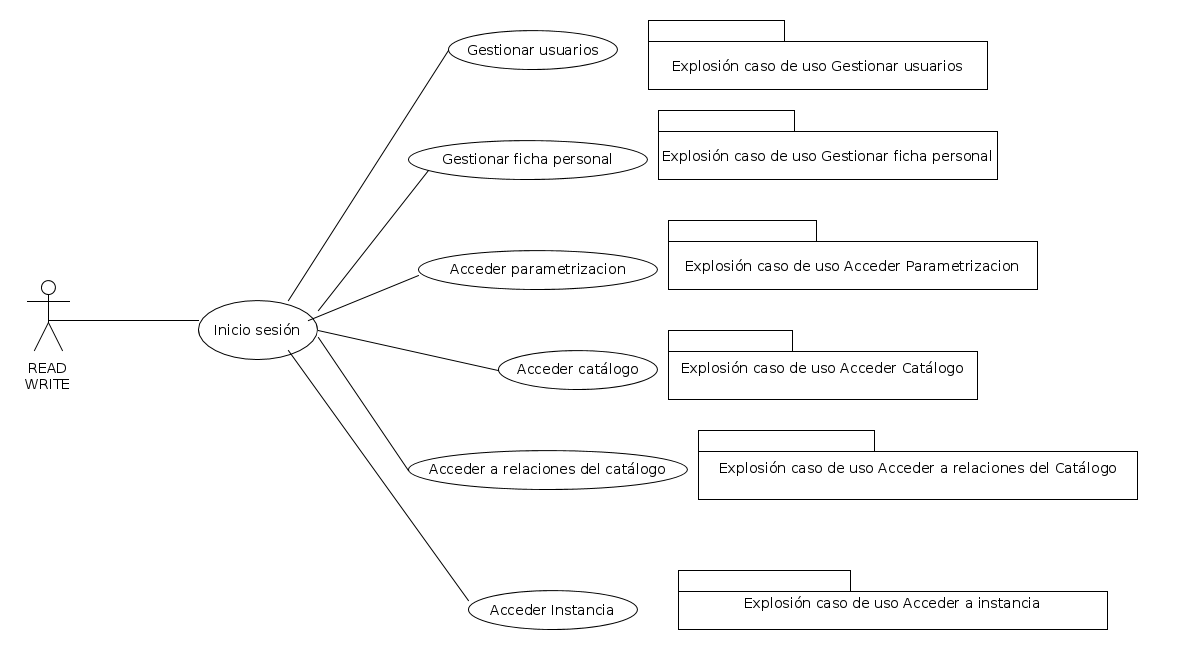
\includegraphics[width=\textwidth]{imaxes/cu-admin.png}
  \caption{Casos de uso del actor ADMIN}
  \label{fig:cu-admin-chap-analisis}
\end{figure}



A continuación se muestra un caso de uso destacable que representa
aspecto centrales de la aplicación. La definición completa de casos de uso se encuentra en el Apéndice~\ref{chap:ref-tecnica}. 

Se trata del caso de uso CU-24 (\tablename~\ref{tab:cu-listar-catálogo-historico-chap-analisis}, página \pageref{tab:cu-listar-catálogo-historico-chap-analisis}) y los casos de uso asociados  CU-05 (\tablename~\ref{tab:cu-editar-historico-chap-analisis}, página \pageref{tab:cu-editar-historico-chap-analisis}), CU-06 (\tablename~\ref{tab:cu-cancelar-historico-chap-analisis}, página \pageref{tab:cu-cancelar-historico-chap-analisis}), CU-07 (\tablename~\ref{tab:cu-anhadir-historico-elemento-chap-analisis}, página \pageref{tab:cu-anhadir-historico-elemento-chap-analisis}) y CU-09 (\tablename~\ref{tab:cu-borrar-historico-elemento-chap-analisis} página \pageref{tab:cu-borrar-historico-elemento-chap-analisis}), que hacen referencia a la modificación de un registro de histórico de una entidad con histórico de registros (como pudiera ser un tipo de cuota). A estos casos de uso pueden acceder los actores WRITE y ADMIN a través del correspondiente caso de uso de listado de la entidad a tratar y seleccionando el correspondiente registro de histórico a modificar.

Para este tipo de entidades con registro de histórico es fundamental que exista una consecución temporal de los mismos. No puede haber registros de histórico que se solapen para una misma instacia de una entidad, ni tampoco \textit{huecos} en la línea temporal del ciclo de vida de la misma. Por lo tanto se debe revisar que los cambios producidos en las fechas de una entidad con registro de histórico sean coherentes con lo almacenado en el sistema, actualizando fechas de registros anteriores y/o posteriores en caso de ser necesario, para \textit{acortarlos} o \textit{alargarlos} según sea el caso.


\begin{table} [H]
    \centering
    \rowcolors{2}{white}{white}
    \setlength{\leftmargini}{0.4cm}
	\resizebox{14cm}{!} { % evita que la tabla sobresalga de la p\'agina, ajustando tama\'no de letra y grosor de l\'ineas
    \begin{tabular}{| m{3cm} | m{11cm} |}   
    \hline
	  \textbf{CU-24} & \textbf{Acceder al catálogo entidad con históricos} \\\hline
	  \textbf{Descripción} & Listar entidad histórica de catálogo seleccionada y gestionar los datos si se tienen los permisos correspondientes. \\\hline
	  \textbf{Actores} & READ, WRITE y ADMIN. \\\hline
	  \textbf{Precondiciones} & El usuario está conectado y ha seleccionado del menú la entidad histórica a listar del catálogo. \\\hline
	  \textbf{Postcondiciones} & Se muestra el listado de históricos de la entidad seleccionada. \\\hline
	  \textbf{Flujo básico} & 
		\begin{enumerate}
	  	\item Se muestran un área de búsqueda con dos opciones, buscar histórico completo o buscar por fecha, y un botón para realizar la búsqueda de la entidad en función del criterio seleccionado.
	  	\item Si el usuario es el actor WRITE o ADMIN se muestra un botón para crear una nueva entidad.
	  	\item Si el cliente pulsa el botón de búsqueda se da paso al caso de uso \ref{tab:cu-buscar-elementos-historico} y a continuación se muestra el listado del elemento seleccionado.
	  	\item Si el usuario es el actor WRITE o ADMIN y selecciona la opción crear nuevo se da paso al \ref{tab:cu-nuevo-elemento} (\pageref{tab:cu-nuevo-elemento} y a continuación se muestra el listado del nuevo elemento creado.
		\item Si el usuario es el actor WRITE o ADMIN, sobre cada registro de histórico se mostrarán tres botones, uno para añadir registro de histórico, otro para editar el registro y otro para borrar el registro. Si el usuario selecciona un registro del listado y
		    \begin{enumerate}
		         \item Pulsa el botón de añadir se da paso al caso de uso \ref{tab:cu-anhadir-historico-elemento} (página \pageref{tab:cu-anhadir-historico-elemento})
		        \item Pulsa el botón de edición se da paso a los casos de uso \ref{tab:cu-editar-historico} (página \pageref{tab:cu-editar-historico}) y \ref{tab:cu-cancelar-historico} (página \pageref{tab:cu-cancelar-historico}).
		        \item Pulsa el botón de borrado se da paso al caso de uso \ref{tab:cu-borrar-historico-elemento} (página \pageref{tab:cu-borrar-historico-elemento}).
		    \end{enumerate} 
		\item Finaliza el caso de uso.
	  \end{enumerate} 	  	  
	  \\\hline
    \end{tabular}
    } % end /resizebox
    \caption{CU-24 Acceder al catálog entidad con históricos}
    \label{tab:cu-listar-catálogo-historico-chap-analisis}
\end{table}




\begin{table} [H]
    \centering
    \rowcolors{2}{white}{white}
    \setlength{\leftmargini}{0.4cm}
	\resizebox{14cm}{!} { % evita que la tabla sobresalga de la p\'agina, ajustando tama\'no de letra y grosor de l\'ineas
    \begin{tabular}{| m{3cm} | m{11cm} |}   
    \hline
	  \textbf{CU-05} & \textbf{Editar registro de histórico del elemento seleccionado} \\\hline
	  \textbf{Descripción} & Editar registro de histórico del elemento seleccionado. \\\hline
	  \textbf{Actores} & WRITE y ADMIN. \\\hline
	  \textbf{Precondiciones} & El usuario con perfil WRITE o ADMIN ha pulsado el botón editar para el registro de histórico para el elemento seleccionado. \\\hline
	  \textbf{Postcondiciones} & Se modifica el registro de histórico elemento del listado de la entidad  y, si es necesario, se modifican las fechas de los regisros registros anterior y posterior para que sean consecutivos. \\\hline
	  \textbf{Flujo básico} & 
		\begin{enumerate}
	  	\item El sistema muestra los campos editables del registro seleccionado y dos botones: guardar y cancelar.
        \item El usuario modifica los campos deseados sobre el registro. Si el estado del registro cambia al estado cancelado se dispara el caso de uso \ref{tab:cu-cancelar-historico} (página \pageref{tab:cu-cancelar-historico}).
			\begin{enumerate}	
			   \item El usuario pulsa el botón de guardar. El sistema comprueba que los campos obligatorios han sido completados y que los datos tienen el formato correcto. Realiza las modificaciones pertinentes en los registros de histórico anterior y posterior del elemento seleccionado, de forma que todos los registros de histórico sean correlativos. Se guardan los datos de fecha de creación y nombre de usuario tanto para el nuevo registro de histórico como para los registros adyacentes modificados. Se termina la edición del registro. Se informa al usuario que el registro ha sido modificado y se actualiza el listado de la entidad con las modificaciones realizadas.
			   \begin{enumerate}	
			   \item  \textit{\textbf{Flujo alternativo:} Si no se cubre algún campo obligatorio o se produce algún error de validación el sistema informa del error.}
			   \end{enumerate}
			   \item El usuario pulsa el botón cancelar. Se termina la edición del registro y se descartan los posibles cambios.
			\end{enumerate}
	  \item Finaliza el caso de uso.
	  \end{enumerate} 	  	  
	  \\\hline
    \end{tabular}
    } % end /resizebox
    \caption{CU-05 Editar histórico de elemento seleccionado}
    \label{tab:cu-editar-historico-chap-analisis}
\end{table}


\begin{table} [H]
    \centering
    \rowcolors{2}{white}{white}
    \setlength{\leftmargini}{0.4cm}
	\resizebox{14cm}{!} { % evita que la tabla sobresalga de la p\'agina, ajustando tama\'no de letra y grosor de l\'ineas
    \begin{tabular}{| m{3cm} | m{11cm} |}   
    \hline
	  \textbf{CU-06} & \textbf{Cancelar el registro de histórico del elemento seleccionado} \\\hline
	  \textbf{Descripción} & Cancelar el registro de histórico del elemento seleccionado. \\\hline
	  \textbf{Actores} & WRITE y ADMIN. \\\hline
	  \textbf{Precondiciones} & El usuario con perfil WRITE o ADMIN ha seleccionado el estado cancelado para el registro de histórico que está modificando. \\\hline
	  \textbf{Postcondiciones} & Se propaga el estado de cancelado para todos los registros de histórico posteriores al registro seleccionado. \\\hline
	  \textbf{Flujo básico} & 
		\begin{enumerate}
	  	\item Se muestra un cuadro de diálogo solicitando propagar el estado cancelado para los registros posteriores al registro de histórico seleccionado.
        \item 
			\begin{enumerate}	
			   \item El usuario pulsa el botón de aceptar. El sistema propaga el nuevo estado al resto de registros de históricos posteriores al registro de histórico seleccionado. Se cierra el cuadro de diálogo.
			   \item El usuario pulsa el botón cancelar. Se cierra el cuadro de diálogo y se descarta el cambio de estado.
			\end{enumerate}
	  \item Finaliza el caso de uso.
	  \end{enumerate} 	  	  
	  \\\hline
    \end{tabular}
    } % end /resizebox
    \caption{CU-06 Cancelar el registro de histórico del elemento seleccionado}
    \label{tab:cu-cancelar-historico-chap-analisis}
\end{table}


\begin{table} [H]
    \centering
    \rowcolors{2}{white}{white}    
    \setlength{\leftmargini}{0.4cm}
	\resizebox{14cm}{!} { % evita que la tabla sobresalga de la p\'agina, ajustando tama\'no de letra y grosor de l\'ineas
    \begin{tabular}{| m{3cm} | m{11cm} |}   
    \hline
	  \textbf{CU-07} & \textbf{Añadir registro de histórico del elemento seleccionado} \\\hline
	  \textbf{Descripción} & Añadir registro de histórico del elemento seleccionado. \\\hline
	  \textbf{Actores} & WRITE y ADMIN. \\\hline
	  \textbf{Precondiciones} & El usuario con perfil WRITE o ADMIN ha pulsado el botón añadir registro de histórico para el elemento seleccionado. \\\hline
	  \textbf{Postcondiciones} & Se añade un nuevo registro de histórico  comprendido entre el elemento seleccionado del listado de la entidad y el siguiente elemento de la lista, o a continuación del elemento seleccionado si no hay más elementos en la lista, modificando las fechas de dichos regisros para que sean consecutivos. \\\hline
	  \textbf{Flujo básico} & 
		\begin{enumerate}
	  	\item El sistema muestra un formulario con una copia del registro de histórico del elemento seleccionado con los campos susceptibles de modificar habilitados. El usuario modificará las fechas de inicio y/o fin del registro, así como el resto de campos que considere oportuno. 
			\begin{enumerate}	
			   \item El usuario pulsa el botón de guardar. El sistema comprueba que los campos obligatorios han sido completados y que los datos tienen el formato correcto. Evalúa las fechas de inicio y fin y realiza las modificaciones pertinentes sobre los histórico anterior y posterior del elemento seleccionado o sólo del anterior en caso de que no hubiera más registros, de forma que todos los registros de histórico sean correlativos. Se guardan los datos de fecha de creación y nombre de usuario para el nuevo registro de histórico, así como los de fecha de modificación y usuario para los registros de histórico adyacentes modificados. Se termina la edición del registro. Se informa al usuario que el elemento ha sido añadido. Se añade el registro al listado de la entidad y se actualiza con las modificaciones realizadas.
			   \begin{enumerate}	
			   \item  \textit{\textbf{Flujo alternativo:} Si no se cubre algún campo obligatorio o se produce algún error de validación el sistema informa del error.}
			   \end{enumerate}
			   \item El usuario pulsa el botón cancelar. Se vuelve al caso de uso inicial \ref{tab:cu-listar-parametrización} (\pageref{tab:cu-listar-parametrización}).
			\end{enumerate}
	  \item Finaliza el caso de uso.
	  \end{enumerate} 	  	  
	  \\\hline
    \end{tabular}
    } % end /resizebox
    \caption{CU-07 Añadir histórico de elemento seleccionado}
    \label{tab:cu-anhadir-historico-elemento-chap-analisis}
\end{table}




\begin{table} [H]
    \centering
    \rowcolors{2}{white}{white}
    \setlength{\leftmargini}{0.4cm}
	\resizebox{14cm}{!} { % evita que la tabla sobresalga de la p\'agina, ajustando tama\'no de letra y grosor de l\'ineas
    \begin{tabular}{| m{3cm} | m{11cm} |}   
    \hline
	  \textbf{CU-09} & \textbf{Borrar histórico del elemento seleccionado} \\\hline
	  \textbf{Descripción} & Borrar histórico elemento seleccionado. \\\hline
	  \textbf{Actores} & WRITE y ADMIN. \\\hline
	  \textbf{Precondiciones} & El usuario con perfil WRITE o ADMIN ha pulsado el botón de borrar para el registro de histórico del elemento selecconado. \\\hline
	  \textbf{Postcondiciones} & Se elimina el registro de histórico del elemento seleccionado, modificando las fechas de los regisros anterior y/o posterior para que sean consecutivos. \\\hline
	  \textbf{Flujo básico} & 
		\begin{enumerate}
	  	\item El sistema muestra un cuadro de diálogo solicitando confirmación de borrado del registro de histórico del elemento seleccionado con dos botones: aceptar y cancelar.
		\item 
			\begin{enumerate}	
			   \item El usuario pulsa el botón de aceptar. El sistema elimina del el registro de histórico del elemento seleccionado y realiza las modificaciones pertinentes en los registros de histórico anterior y posterior del elemento seleccionado, de forma que todos los registros de histórico sean correlativos. Se informa al usuario que el elemento ha sido borrado. Se elimina el elemento del listado de la entidad  y se actualiza con las modificaciones realizadas. Se cierra el cuadro de diálogo.
			   \begin{enumerate}	
			   \item  \textit{\textbf{Flujo alternativo:} Si se produce algún error el sistema informa del error.}
			   \end{enumerate}
			   \item El usuario pulsa el botón cancelar. Se vuelve al caso de uso inicial \ref{tab:cu-listar-parametrización} (\pageref{tab:cu-listar-parametrización}).
			\end{enumerate}
	  \item Finaliza el caso de uso.
	  \end{enumerate} 	  	  
	  \\\hline
    \end{tabular}
    } % end /resizebox
    \caption{CU-09 Borrar histórico del elemento seleccionado}
    \label{tab:cu-borrar-historico-elemento-chap-analisis}
\end{table}




\section{Diseño}
\label{sec:disenho}

En esta sección describiremos los distintos elementos usados para el diseño de la aplicación.


\subsection{Arquitectura en tres niveles}
\label{sub:arquitectura3niveles}

Para el desarrollo de este proyecto se ha optado por el patrón de arquitectura \acrlong{mvc} que presenta una arquitectura que separa las aplicaciones en tres niveles \footnote{Aunque está comunmente aceptado capa como sinónimo de nivel, no significan lo mismo. Una \textit{\textbf{capa}} se refiere a una \textit{división funcional del software}, pero un \textit{\textbf{nivel}} se refiere a una \textit{división funcional del software que se ejecuta en una infraestructura separada}  de las otras divisiones, por lo que las capas no pueden ofrecer los mismos beneficios que los niveles}: la interfaz de usuario, el nivel donde se procesan los datos y el nivel donde se almacenan y gestionan esos datos ~\cite{ibmMVC} (ver \figurename~\ref{fig:arquitectura-3-niveles}).

\begin{figure}
  \centering
  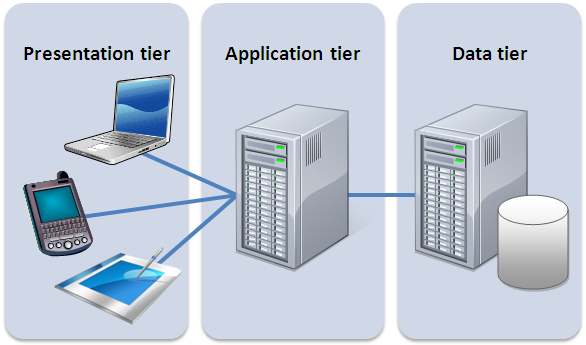
\includegraphics[width=0.55\textwidth]{imaxes/arquitectura-3-niveles.png}
  \caption{Representación de la arquitectura en tres niveles}
  \label{fig:arquitectura-3-niveles}
\end{figure}


El propósito de cada una de ellas es el siguiente:
\begin{itemize}
\item \textbf{Nivel de presentación}. Es la interfaz de usuario, donde el usuario final interactúa con la aplicación. Este primer nivel puede ejecutarse en una navegador web como una aplicación de escritorio o una \acrshort{gui}.
\item \textbf{Nivel de aplicación}. También conocido como el \textit{nivel lógico o medio}, es el núcleo de la aplicación. Se procesa la información recogida en el nivel de presantación. En ocasiones este procesado de información se realiza junto con otra información en el nivel de datos a través de lo que se conoce como  lógica empresarial: un conjunto específico de reglas empresariales. Este nivel también puede añadir, suprimir o modificar datos en el nivel de datos. Se comunica con el nivel de datos mediante llamadas a las distintas \acrshort{api}. 
\item \textbf{Nivel de datos}. También denominado nivel de base de datos, de acceso a datos o backend, es donde se almacena y gestiona la información procesada por la aplicación. Puede ser un sistema de gestión de base de datos relacional (PostgreSQL, MySQL, Oracle,\dots) o en un servidor de bases de datos NoSQL (MongoDB, Cassandra,\dots). \newline
\end{itemize}


En una aplicación de tres niveles, toda la comunicación pasa por el nivel de aplicación. Los niveles de presentación y de datos no pueden comunicarse directamente entre sí.

La arquitectura de tres niveles aporta múltiples ventajas~\cite{ibmMVC}:
\begin{itemize}
\item Desarrollo más rápido: debido a que cada nivel puede ser desarrollado simultáneamente por diferentes equipos, una empresa puede llevar su aplicación al mercado más rápido y los programadores pueden utilizar los mejores y más recientes lenguajes y herramientas para cada nivel.
\item Escalabilidad mejorada: cualquier nivel se puede escalar independientemente de los demás según sea necesario.
\item Confiabilidad mejorada: es menos probable que una interrupción en un nivel afecte la disponibilidad o el rendimiento de los otros niveles.
\item Seguridad mejorada: debido a que los niveles de presentación y de datos no se pueden comunicar directamente entre sí, un nivel de aplicación bien diseñado puede funcionar como una especie de firewall interno, lo que impide ataques de inyecciones SQL y otras vulnerabilidades maliciosas.
\end{itemize}


\subsection{Patrones utilizados}
\label{sub:patrones}

A continuación se listan algunos de los patrones utilizados en el diseño de la herramienta presentada.



\paragraph{Patrón modelo vista controlador}
El framework \acrshort{jsf} se basa en el patrón \acrlong{mvc}.

Aunque el patrón \acrshort{mvc} comparte con la arquitectura de tres niveles la visión de la apliación en 3 áreas separadas, difiere en la forma de entender la comunicación entre ellas: en el patrón de modelo vista controlador las distintas capas se comunican de forma triangular, dos a dos, mientras que en la arquitectura de tres niveles toda comunicación pasa por el nivel de aplicación.
\begin{itemize}
\item \textbf{Nivel de persistencia}. Recibe solicitudes de almacenamiento o recuperación de información por parte del nivel de negocio, es decir, es la encargada de cargar y modificar la información guardada en el servidor de base de datos. Se encarga de convertir los datos de los registros de la base de datos a objetos manejables por Jakarta EE, para lo que cuenta con un mecanismo de conversión de datos relacionales a objetos. 
\item \textbf{Nivel de negocio}. Se encarga de las reglas del negocio que resuelve o satisface las necesidades de un dominio en un negocio particular. En este nivel se encuentra en el servidor de aplicaciones. Los componentes de este nivel interactúan con el nivel de persistencia y suelen implementarse como componentes EJB.
\item \textbf{Nivel de presentación}. Se encarga de interactuar con el usuario final. Contiene la lógica de presentación que se emplea para generar una respuesta al cliente y sus operaciones son soportadas por el contenedor web que es el encargado de dar un acceso visual al sistema a través de una interfaz de usuario como la web a través de un navegador. Este nivel utiliza el nivel de negocio para realizar ciertas operaciones.
\end{itemize}


\begin{figure}[H]
  \centering
  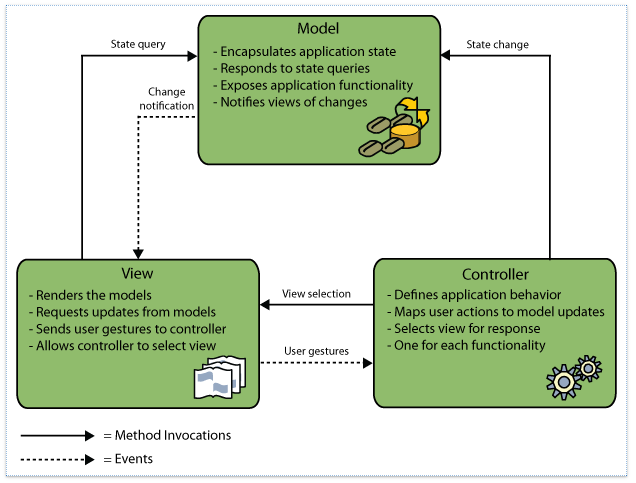
\includegraphics[width=0.6\textwidth]{imaxes/mvc-patron.png}
  \caption{Diagrama del patron MVC donde se observan los distintos niveles y la comunicación entre ellos.}
  \label{fig:patron-mvc}
\end{figure}




    
\paragraph{Composite View}
El sistema de plantillas de JSF se basa en el patrón de diseño Composite View,
lo que significa que las secciones de una página o incluso las propias páginas pueden ser reutilizadas por otras páginas.
Se han utilizado plantillas en el diseño de la ventana principal de la aplicación, la barra de herramientas de la aplicación que contiene el acceso al menú y a la información del usuario, así como la información de la vista actual.


\paragraph{DTO - Data Transfer Object}
Se utiliza este patrón para reducir el número de llamadas a métodos mediante el uso de objetos que transportan datos entre procesos. También permite la encapsulación de la lógica de la serialización (el mecanismo que traduce la estructura del objeto y los datos a un formato específico que se puede almacenar y transferir) proporcionando un único punto de cambio en los matices de serialización.

Los objetos de este patrón generalmente se crean como \acrlong{pojo}. Se trata de estructuras de datos planas que no contienen lógica de negocio, sólo  almacenamiento, accesorios y, finalmente, métodos relacionados con la serialización o el análisis.


\paragraph{DAO - Data Access Object}
Se usa este patrón para abstraer y encapsular todos los accesos al almacén de datos persistente, gestionando la conexión con el origen de datos para obtener y almacenar los datos. 
Este patrón ha sido utilizado en la herramienta para insertar, modificar y borrar los distintos datos de la base de datos.



 
 \chapter{Implementación}
\label{chap:implementacion}


\lettrine{E}{n} este capítulo se detallan los detalles técnicos necesarios para llevar a cabo la implementación de la aplicación.


\section{Hardware Utilizado}
\label{sec:hw}
El proyecto fue desarrollado sobre un equipo con las siguientes características:

\begin{itemize}
\item Procesador: Intel® Core™ i7-1195G7, 2.90GHz × 8
\item Memoria: 16,0 GiB
\item Disco Duro: 1,0 TB
\end{itemize}
	

\section{Software Utilizado}
\label{sec:sw}	

 UBUNTU 22.04.1 LTS y 22.04.1 LTS\\
 Sistema operativo sobre el que se desarrolló la aplicación.
 \\	 
 
 WILDFLY 20.0.1\\
 Servidor de aplicaciones \acrshort{jee} de \gls{opensource}, utilizado para la implantación de la aplicación web.
 \\
 
 MOZILLA FIREFOX 104.0\\
 Navegador web usado para la ejecución y pruebas de la aplicación web.
 \\ 
 
 ECLIPSE 4.16 2020-06\\
 \acrfull{ide} \gls{opensource} utilizado para la generación del código de la aplicación .
 \\
 
 JAKARTA EE 8.0 (y JAVA SE 1.8.0)\\
 Lenguaje de programación utilizado para desarrollar la aplicación.
 \\
 
 MAVEN 3.6.3
 Herramienta de software de \gls{opensource} para la gestión y construcción de proyectos Java.
 \\

 
 POSTGRESQL 14.5\\
 \acrshort{sgbd} de \gls{opensource} utilizado como soporte de almacenamiento.
 \\
 
 DBeaver 22.1.4\\
 Herramienta gráfica \gls{opensource} de diseño y gestión de bases de datos, utilizada para gestionar la base de datos creada para la aplicación.
 \\

 SCHEMASPY 5.0.0\\
 Herramienta basada en Java que genera representaciones visuales de un esquema de base de datos en un formato visible por el navegador.
 \\ 
 
 UMLET 15.0\\
 Herramienta \gls{opensource} para la modelización de diagramas \acrshort{uml}.


 
 UMBRELLO 2.35.0\\
 Programa para desarrllollar diagramas en \acrfull{uml} basado en tecnología KDE.
 \\
 
 \LaTeX{}\\
 Sistema de composición de textos utilizado para generar el presente documento.
 \\ 
 
 TEXMAKER 5.0.3\\
 Editor \LaTeX{} para redactar el presente documento.
 
 
 

	
 
 \chapter{Planificación temporal y estimación de costes}
\label{chap:planificacion}

Tan importante como la estimación económica del proyecto es la planificación temporal del mismo. La duración de cada activida del proyecto vendrá dada por múltiples factores entre ellos la complejidad, el esfuerzo requerido y el tiempo disponible.

Del equilibrio entre ambos factores depende en buena parte la viabilidad del
proyecto. Por ello, es necesario realizar un estudio del tiempo que se va a dedicar a cada fase y un análisis económico. Una buena gestión maximiza la probabilidad de consecución de resultados a tiempo, dentro de presupuesto y con la calidad esperada.

A continuación se presenta la planificación temporal y la estimación de costes de nuestro proyecto.

\section{Fases del proyecto} 

La planificación se ha realizado desglosando el proyecto en seis fases o tareas: análisis, diseño, codificación, pruebas, documentación y memoria. 

La duración de cada actividad del proyecto viene dada por múltiples factores, entre ellos la curva de aprendizaje de las tecnologías utilizadas para cada actividad, la complejidad de los problemas a resolver y los contratiempos que han surgido en cada etapa.

Para la realización del proyecto, por circunstancias personales se ha establecido un horario de 28 horas semanales, salvo para el último mes que han sido de 40 horas semanales. En aquellos casos en que las actividades se solapan, para facilitar los cálculos, se ha supuesto que el tiempo dedicado a cada una de ellas ha sido equivalente. Cada cuadro sombreado de la gráfica mostrada en la \figurename~\ref{fig:planificacion} corresponde aproximadamente a una semana de trabajo.


\begin{figure}[H]
  \centering
  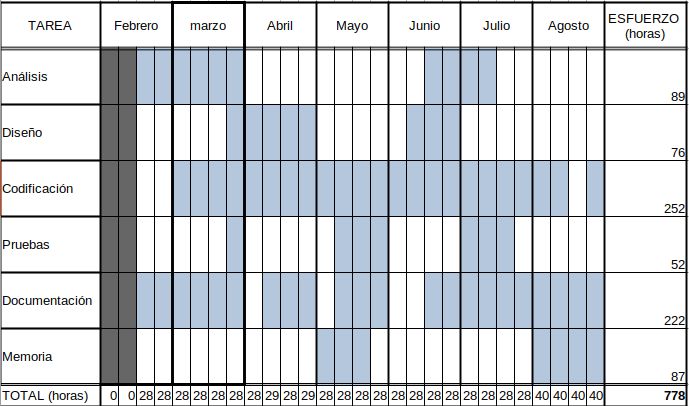
\includegraphics[width=0.9\textwidth]{imaxes/planificacion.png}
  \caption{Tabla de tiempos de planificación del proyecto}
  \label{fig:planificacion}
\end{figure}


\section {Costes estimados}

Este trabajo ha requerido aproximadamente 776 horas de trabajo personal que
podríamos valorar en 15.520 € a razón de 20 €/hora. A este coste habría que añadir el coste del esfuerzo dedicado por el director del proyecto, software, equipo, y otros gastos generales como electricidad, conexión a Internet, etc.

Si el proyecto fuese llevado a cabo por un equipo multidisciplinar, el coste laboral total dependería de la categoría de cada integrante atendiendo a su cualificación profesional. Podría estar formado por:
\begin{itemize}
\item Consultor, que se encarga de las líneas de investigación del
departamento.
\item Ingeniero Senior, con funciones de dirección de proyecto.
\item Ingeniero Junior, con una experiencia menor de cinco años.
\item Técnicos Informáticos.
\item Personal Auxiliar.
\end{itemize}

A los costes laborales habría que añadir los derivados de: material y equipo (hardware, consumibles, etc.), costes generales (luz, teléfono, Internet, impuestos) así como otros gastos no reflejados en los apartados anteriores.


%\include{contido/...}
 \chapter{Conclusións}
\label{chap:conclusions}

\lettrine{E}{n} este \acrshort{tfg} se ha desarrollado una herramienta para la gestión del catálogo de servicios y contratación de una cartera de clientes para una empresa proveedora de servicios, alcanzándose los principales objetivos que se pretendían al comienzo de su realización:

\begin{itemize}
\item Se ha implementado una aplicación con acceso vía web que abarca los principales componentes que conforman el sistema: catálogo de servicios, contrataciones y la parametrización necesaria para la configuración de estos elementos.

\item La herramienta permite una gestión de usuarios para implementar el control de acceso o modificación de la información.

\item Se definen distintos niveles de acceso a las funcionalidades de la aplicación en función de distintos perfiles de usuario, lo que evita accesos inadecuados a determinadas funcionalidades del sistema.

\item A la hora de manejar entidade con histórico se realiza una correcta gestión de las fechas de inicio y fin de los mismos de forma que queda garantizada la no existencia de \textit{huecos} entre registros históricos para una misma entidad o instancia (es decir, todos los registros comprendidos entre la fecha mínima de inicio y la máxima de fin son consecutivos).

\item Permite gestionar las diferentes relaciones de dependencia de entidades del catálogo de servicios con un sólo click.

\item Permite búsquedas sencillas para establecer las relaciones de dependencia de las distintas contrataciones a realizar.

\end{itemize}


A esto hay que sumar el cumplimiento de los objetivos personales de ampliar mis conocimientos en distintas áreas técnicas como la de iniciar una aplicación web desde cero con \acrshort{jee} o gestionar una base de datos completa.



\section{Líneas futuras}
\label{sec:futuro}

La herramienta aquí presentada es un prototipo cuyo principal objetivo es la puesta en escena de las principales funcionalidades descritas para la herramienta de contratación. Con vistas a la difusión de una herramienta como la propuesta sería interesante mejorar, o desarrollar en algunos casos, los siguientes aspectos:

\begin{itemize}
\item Mejorar el entorno gráfico para que resulte más agradable y atractivo.
\item Mejorar la experiencia de los usuarios añadiendo opciones de personalización de la interfaz.
\item Incluir la funcionalidad de extracción de informes útiles para departamentos como márketing como pudiera ser volumetrías de clientes dados de alta en un período determinado o productos más contratados.
\item Incluir un canal de comunicación (por ejemplo procesos batch que generan o cargan ficheros de datos) con los distintos sistemas con los que se comunica dentro del área comercial de la empresa, como pudieran ser los sistemas de provisión y facturación, de forma que exista un flujo de información que garantice una correcta alineación en los sistemas del estado de los datos implicados (contrataciones pendientes de provisión, finalización de provisión, suspensión por impago,\dots).
\item Incluir la posibilidad de presentar la aplicación en distintos idiomas mediante la internalización de java.
\end{itemize}


 %%%%%%%%%%%%%%%%%%%%%%%%%%%%%%%%%%%%%%%%
 % Apéndices, glosarios e bibliografía  %
 %%%%%%%%%%%%%%%%%%%%%%%%%%%%%%%%%%%%%%%%

 \appendix
 \appendixpage
 \chapter{CoMaSw. Manual de la Aplicación}
\label{chap:manual}

\lettrine{CoMaSw} (\emph{\textbf{Co}}ntract \emph{\textbf{Ma}}nagement \emph{\textbf{S}}of\emph{\textbf{w}}are) una aplicación de código abierto desarrollada bajo licencia \acrfull{licencia}.


Se trata de un software para la gestión de la contratación de cualquier empresa cuyo modelo de negocio se base en suscripciones con tarifas periódicas (proveedores de servicios, gimnasios, academias, etc.). Las dos actividades principales de esta herramienta son:
\begin{itemize}
\item La gestión del catálogo de servicios de la empresa, mediante la definición de nuevos productos y servicios, elementos facturables como cuotas de consumo y aplicación de descuentos a través de promociones o modificación de las ya existentes.
\item La gestión de la cartera de clientes, creando nuevos clientes o modificando clientes existentes y estableciendo las contrataciones oportunas de los distintos elementos ofertados por la empresa para esos clientes.
\end{itemize}

Para mayor flexibilidad se han definido una serie de elementos parametrizables cuyo objetivo es dotar de mayor adaptabilidad a las entidades ante nuevas necesidades que puedan surgir en el futuro.


\section{Manual del administrador}
\label{sec:manual-administrador}

En esta sección veremos todo lo relacionado con la administración de la aplicación: instalación y gestión de usuarios.

\subsection{Instalación}
\label{sub:instalacion}

\subsubsection{Requisitos hardware y software}
\label{sub:requisitos}

Los requisitos hardware y software para garantizar el funcionamiento correcto de
la aplicación son los que se indican a continuación, aunque es posible que funcione
sobre un hardware con características inferiores y con otras versiones de los requisitos
software no está garantizada la compatibilidad.
\begin{itemize}
\item \textbf{REQUISITOS HARDWARE}\newline
Los requisitos hardware son los generales para un servidor de base de datos y un servidor web básico. Dependiendo del número de usuarios y del volumen de datos será necesario aumentar el número de recursos.
Requisitos mínimos de instalación:
	\begin{itemize}
	\item Memoria: 8 GB
	\item Disco Duro: 30 GB de espacio libre.
	\end{itemize} 

\item \textbf{REQUISITOS SOFTWARE}\newline
Los requisitos software necesarios para ejecutar la aplicación son los siguientes:
	\begin{itemize}
		\item \textit{\textbf{Servidor}}
		\begin{itemize}
			\item Servidor web: Wildfly 20.0.1
			\item Sistema gestor de bases de datos: PostgreSQL 14.5
		\end{itemize}

		\item \textit{\textbf{Cliente}}
		\begin{itemize}
			\item Navegador web: Mozilla Firefox 104.0.1, Chromium 105.0.5195.52
		\end{itemize}
	\end{itemize}
\end{itemize}




\subsubsection{Procedimiento de instalación}
\label{sub:proceso-instalacion}
A continuación se detallan los pasos a seguir para el proceso de instalación (nota: Antes de comenzar la instalación, revisar que el software necesario esté instalado y configurado correctamente).
\begin{enumerate}
\item \underline{\textbf{Descomprimir el fichero \emph{comasw\_files.zip}}} \newline
Este fichero comprimido contiene lo siguiente:
	\begin{itemize}
	    \item readme.txt - fichero con los pasos a realizar para la instalación (los mismos que aquí se describen).
		\item CoMaSw.war - fichero war de la aplicación.
		\item postgresql-42.4.1.jar - driver jdbc para postgres.
		\item creacion\_db.sql - script con los pasos necesarios para la creación de la base de datos.
		\item db\_comasw.sql - fichero de importación de la base de datos.
	\end{itemize}

\item \underline{\textbf{Configurar la base de datos}}\newline
La base de datos de la aplicación se llama \emph{\textbf{db\_comasw}} y tiene dos usuarios:
	\begin{itemize}
		\item \emph{comasw\_admin} - usuario propietario de la base de datos. Todo nuevo objeto a crear en la base de datos de la aplicación deberá crearse con este usuario.
		\item \emph{comasw\_app} - usuario de la aplicación CoMaSw (con el que establece conexión la aplicación a la base de datos). En caso de crear nuevos objetos en la base de datos relacionados con la aplicación deberán otorgársele los permisos correspondientes a este usuario sobre dichos objetos.
	\end{itemize}
\underline{\textbf{Por seguridad se recomienda cambiar las contraseñas de los usuarios comasw\_admin y comasw\_app}}.
A continuación se describen los pasos a seguir para crear y configurar la base de datos.	
	\begin{enumerate}
		\item \underline{\textbf{Crear la base de datos \emph{\textbf{db\_comasw}}}}\\
Desde la ruta en la que hemos descomprimido el fichero nos conectaremos a la base de datos de postgresql y ejecutamos lo siguiente:
\begin{lstlisting}[style=comando]
  $ creacion_db.sql
\end{lstlisting}

	\item \underline{\textbf{Importar la base de datos \emph{\textbf{db\_comasw}}}}.\\
Desde el terminal nos colocamos en la ruta en la que hemos descomprimido el fichero y ejecutamos lo siguiente:
\begin{lstlisting}[style=comando]
  $ psql -U postgres db_comasw < db_comasw.sql
\end{lstlisting}

	\end{enumerate}
\item \underline{\textbf{Configurar el servidor web Wildfly}}\newline
A través del CLI de Wildfly ejecutar lo siguiente:

	\begin{enumerate}
	\item  \underline{\textbf{Desplegar el driver JDBC}}\newline
Ejecutamos lo siguiente, siendo \textbf{[ruta\_driver]} la ruta en la que hemos ubicado el driver contenido en el fichero \emph{comasw\_files.zip}:
\begin{lstlisting}[style=comando]
  module add --name=org.postgresql --resources=(*\bfseries[ruta\_driver]*)/postgresql-42.4.1.jar --dependencies=javax.api,javax.transaction.api
\end{lstlisting}

	\item \underline{\textbf{Asociar el driver JDBC}}\newline
Ejecutamos lo siguiente:
\begin{lstlisting}[style=comando]
/subsystem=datasources/jdbc-driver=postgres:add( driver-name="postgres", driver-module-name="org.postgresql", driver-class-name=org.postgresql.Driver)
\end{lstlisting}

\item \underline{\textbf{Añadir la base de datos db\_comasw con el usuario de la aplicación comasw\_app}}\newline
Ejecutamos lo siguiente, cambiando [comasw\_app] por la nueva contraseña del usuario comasw\_app asignada en la configuración de la base de datos:
\begin{lstlisting}[style=comando]
data-source add --name=db\_comasw --driver-name=postgres --jndi-name=java:jboss/datasources/db\_comasw --connection-url=jdbc:postgresql://localhost:5432/db\_comasw --user-name=comasw\_app --password=[comasw\_app] --enabled=true
\end{lstlisting}
	\end{enumerate}

\item \underline{\textbf{Copiar el fichero comasw.war a la carpeta de aplicaciones de Wildfly}}
\item \underline{\textbf{Desplegar la aplicación en el servidor}}
\end{enumerate}


 
\subsection{Acceso}
\label{sub:acceso-administrador}
 
Para acceder a la aplicación escribir en la barra de direcciones de la aplicación la
siguiente URL: {\footnotesize \tt http://[servidor]:8080}, donde servidor es el nombre del servidor web.

La aplicación utiliza usuarios para el control de acceso y para auditar la
modificación de la información almacenada.

Las credenciales establecidas por defecto para el usuario administrador son ADMIN/ADMIN como nombre de usuario/contraseña. Por razones de seguridad es recomendable que una vez iniciada la sesión se cambie la contraseña del usuario administrador.
 
 
 
\subsection{Gestión de usuarios}
\label{sub:gestion-usuarios}

Cualquier usuario con perfil ADMIN puede gestionar las altas, bajas y modificaciones de otros usuarios del sistema. Los usuarios con este perfil tienen habilitado un botón \emph{Configuration} situado en la esquina superior derecha de la aplicación, que al pulsarlo despliega un menú con una única opción Manage Users (\figurename~\ref{fig:boton-gestion-usuarios}):

\begin{figure}[H]
  \centering
  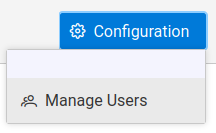
\includegraphics[width=0.25\textwidth]{imaxes/gestion-usuarios-01.png}
  \caption{Acceso a la pantalla de gestión de usuarios}
  \label{fig:boton-gestion-usuarios}
\end{figure}


Cada usuario tendrá asociado un perfil que define los permisos que tiene sobre la aplicación:
\begin{itemize}
\item \textbf{ADMIN} - permisos de administrador. Los usuarios con este perfil puede realizar altas, bajas y modificaciones de cualquier entidad de la aplicación: elementos de la parametrización, del catálogo, de la contratación o los usuarios del sistema.
\item \textbf{ADMIN} - permisos de lectura/escritura. Los usuarios con este perfil puede realizar altas, bajas y modificaciones de las entidades del catálogo del servicio, así como de las contrataciones, y únicamente consultar las entidades de la parametrización. No tienen habilitado el acceso a la gestión de usuarios.
\item \textbf{READ} - permisos de solo lectura. Los usuarios con este perfil sólo pueden consultar los datos de la aplicación correspondientes a la parametrización, el catálogo o la contratación. No tienen habilitado el acceso a la gestión de usuarios.
\end{itemize}


Una vez seleccionado se nos mostrará el listado de todos los usuarios del sistema (\figurename~\ref{fig:listado-usuarios}).
Desde ahí se pueden gestionar las siguientes operaciones:
\begin{description}
\item[\underline{\textsl{\textbf{Crear nuevo usuario}}}] Para crear un nuevo usuario se pulsará el botón \emph{New Data} situado en la parte superior de la tabla. Aparecerá una ventana emergente que mostrará un formulario con los campos a cubrir, entre ellos el perfil con el que se va a crear el usuario y que definirá los permisos de este sobre los elementos de la aplicación.

\item[\underline{\textsl{\textbf{Editar usuario}}}] Para editar un usuario se seleccionará del listado y se pulsará el botón editar de la columna \emph{EDIT ROW}. Se editarán los campos pertinentes de la tabla para realizar las modificaciones oportunas. 

\item[\underline{\textsl{\textbf{Borrar usuario}}}] Para borrar un usuario se seleccionará del listado y se pulsará el botón amarillo de borrar de la columna \emph{DEL ROW} correspondiente.
\end{description}


\begin{figure}[H]
  \centering
  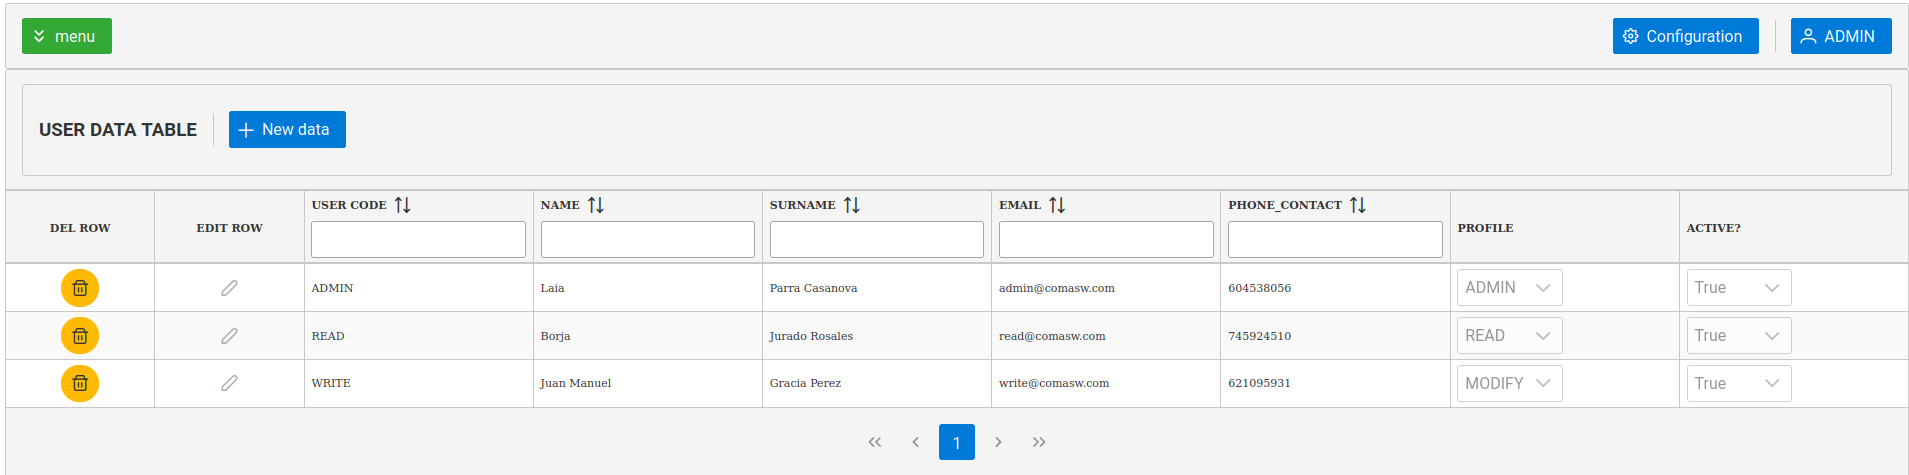
\includegraphics[width=\textwidth]{imaxes/gestion-usuarios-02.png}
  \caption{Listado de usuarios}
  \label{fig:listado-usuarios}
\end{figure}



\section{Manual de usuario}
\label{sec:manual-usuario}

En esta sección se mostrará toda la información necesaria para conocer el funcionamiento por parte del usuario de CoMaSw.


\subsection{Introducción}
\label{sub:introduccion}

Antes de explicar cómo usar \emph{CoMaSw} veamos la visión de contratación que propone la aplicación y los elementos que la conforman.



\subsubsection{Conceptos relativos a las contrataciones}
\label{sub:contratacion-conceptos}

Una contratación es una estructura jerárquica en la que el que la \textit{cabeza} de la misma es el cliente. Dicho cliente puede tener una o más cuentas asociadas. Cada una de estas cuentas es responsable de la contratación de un conjunto de productos, servicios, cuotas y promociones ofertados por la empresa. La \figurename~\ref{fig:estructura-contratacion} muestra dicha estructura de contratación. Vamos a introducir algunos conceptos al respecto.

\begin{figure}
  \centering
  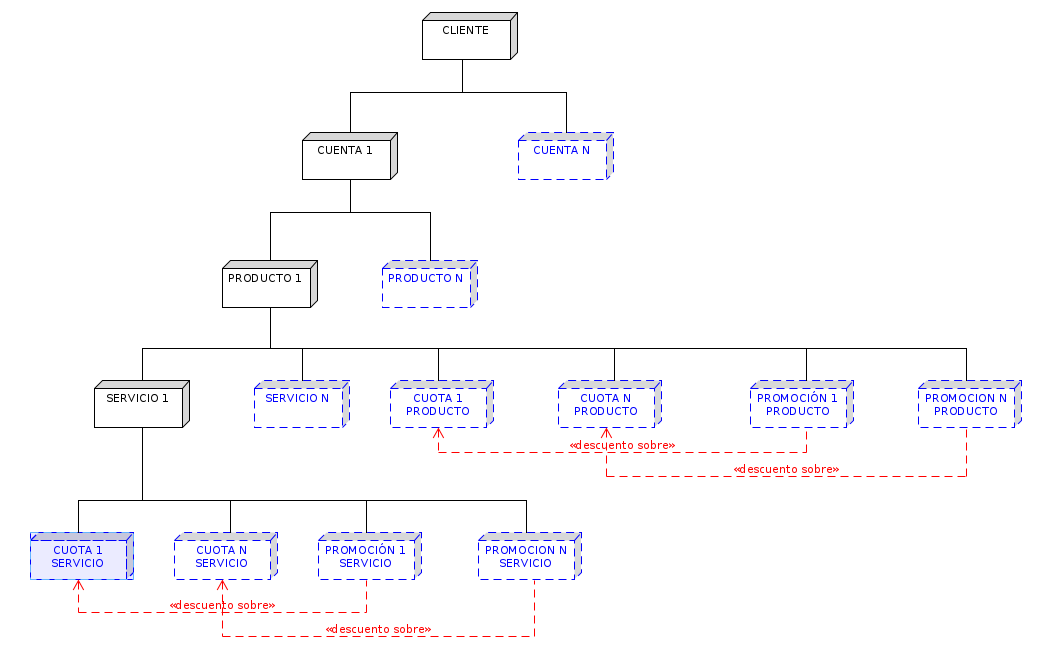
\includegraphics[width=\textwidth]{imaxes/estructura-contratacion.png}
  \caption{Estructura de la contratación}
  \label{fig:estructura-contratacion}
\end{figure}

\paragraph{Cliente.} Por cliente entendemos la persona física (particular o autónomo) o persona jurídica que adquiere los bienes y servicios proporcionados por la empresa a cambio de una transacción monetaria. Es el responsable último de la contratación de los servicios.

\paragraph{Cuenta.} Por cuenta entendemos la entidad del sistema que permite gestionar los distintos productos y servicios contratados por el cliente y es la responsable de la transacción económica asociada a la contratación, esto es, el \textit{pagador}, por lo que tendrá asociada una persona física o jurídica que es la que efectuará el pago y que puede coincidir con el cliente o ser otra distinta. Por lo tanto el ciclo de facturación que aplicará sobre los distintos elementos contratados vendrá dado por la cuenta asociada a los mismos.

\paragraph{Entidad facturable.} Por entidad facturable entendemos todo aquel elemento del sistema susceptible de generar un cargo facturable, y por lo tanto ha de tener un tipo impositivo asociado a la generación de estos cargos, de acuerdo con la ley vigente. Los cargos facturables se denomina elementos facturables y se clasifican en dos tipos:
\begin{itemize}
	\item \emph{\textbf{Cuotas}}: son los elementos que definen los cargos fijos a aplicar sobre las distintas entidades contratadas. Puede tratarse de un cargo que se emite una única vez durante el ciclo de vida de la entidad facturable (por ejemplo la cuota de alta) o cargos periódicos asociados a la prestación de servicios (por ejemplo la cuota mensual).
	\begin{itemize}
		\item Al hablar de cuotas aparece el concepto de \textbf{prorrateable}. Una cuota prorrateable es aquella para la que a la hora de calcular el cargo asociado a la misma durante la facturación se tiene en cuenta el tiempo en el que ha estado vigente dicha cuota: 
		\begin{itemize}
			\item si ha estado en vigencia durante todo el período de facturación se 		facturará el importe completo de la misma.
			\item si ha estado en vigencia sólo una parte del período de facturación se facturará la parte correspondiente a esa vigencia. 
		\end{itemize}
	\end{itemize}
	\item \emph{\textbf{Consumos}}: son los elementos que definen los cargos asociados a los distintos consumos que puede realizar el cliente bajo demanda y que, a diferencia de las cuotas, son importes variables sujetos a la naturaleza de los mismos y al comportamiento propio del consumidor en la demanda de los bienes ofertados. Un ejemplo de este tipo de consumos serían las llamadas de teléfono no incluidas en ningún plan de descuento. El importe a facturar por las llamadas dependerá de varios factores como el número de llamadas realizadas por el cliente, la duración de las mismas o el día y hora a las que las realice.
\end{itemize}


\paragraph{Producto.} Un producto es una entidad facturable conformada por el conjunto de servicios facturables y los posibles descuentos a aplicar sobre los distintos elementos facturables. Es el \textit{paquete} que la empresa oferta a sus clientes. Los únicos elementos facturables que se pueden aplicar sobre este tipo de entidad son del tipo cuota, y por lo tanto los descuentos a aplicar sólo afectarán a dichos cargos facturables.

\paragraph{Servicio.} Un servicio es otra entidad facturable que representa el bien inmaterial que se le presta al cliente y que es el verdadero objetivo de la contratación. Sobre este tipo de entidad pueden aplicarse tanto cuotas como consumos  y por lo tanto los descuentos a aplicar pueden afectara ambos tipos de elementos facturables.

\paragraph{Promoción.} Se entiende por promoción aquella entidad encargada de aplicar los descuentos previamente definidos sobre los distintos elementos facturables.



\subsubsection{Conceptos relativos al catálogo}
\label{sub:catálogo-conceptos}


Para llevar a cabo las distintas contrataciones deberemos saber qué características puede tener cada uno de los elementos que intervienen y elegir unas u otras en función de las necesidades que presenta el cliente. Estas características vienen definidas por unas entidades \textit{plantillas} denominadas tipos que se encuentran englobadas dentro de lo que damos en denominar catálogo. En la \figurename~\ref{fig:estructura-catalogo} se muestra la estructura que define el catálogo de servicios de la aplicación y su implementación en una contratación de los mismos.

\begin{figure}[H]
  \centering
  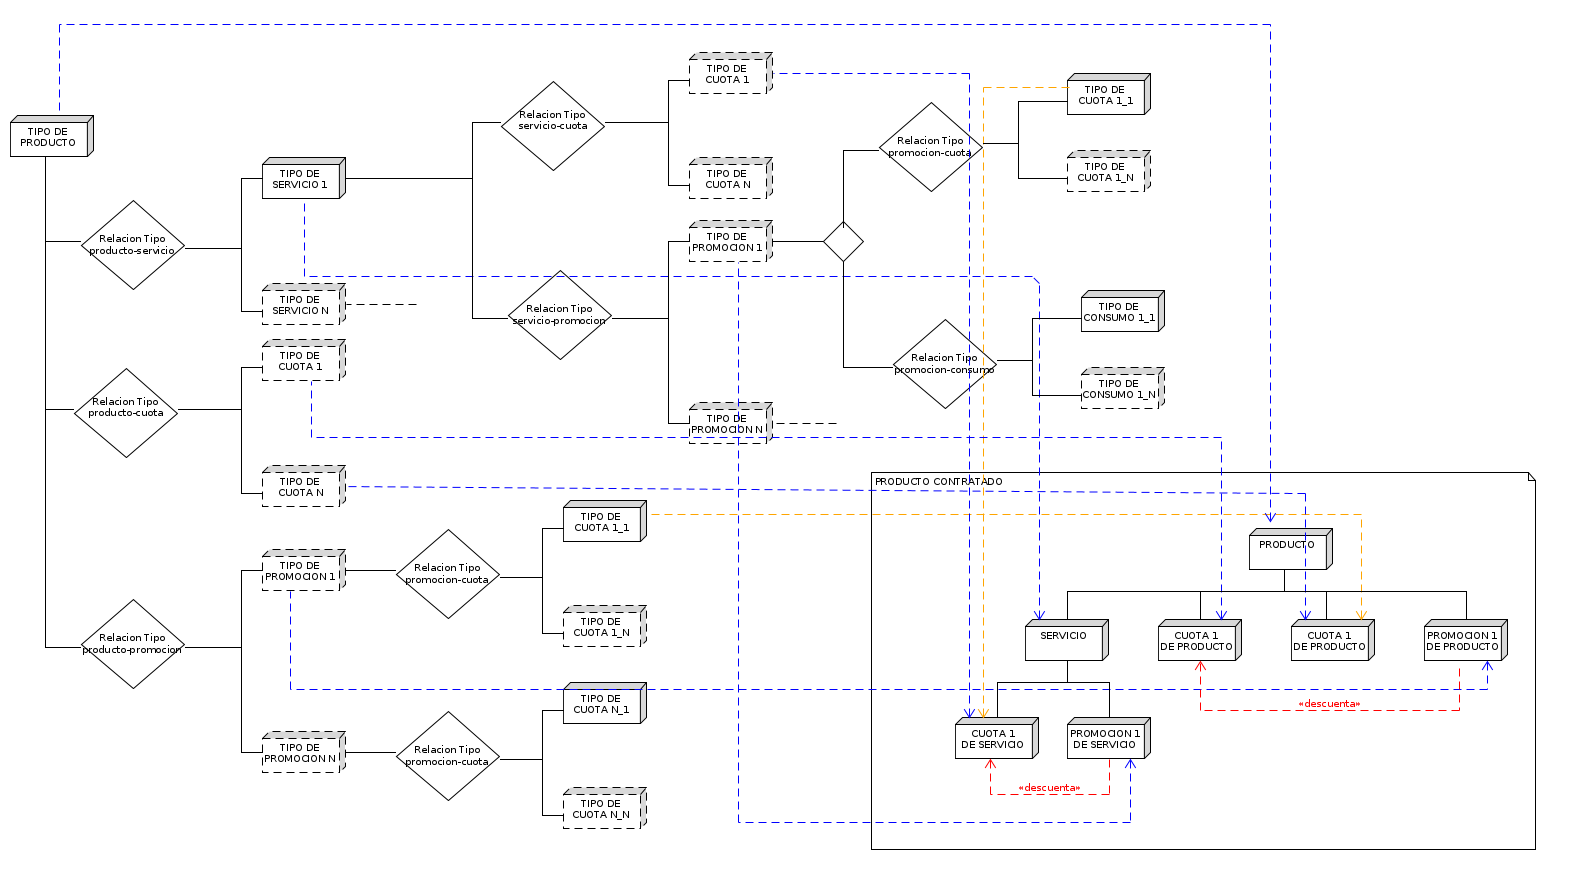
\includegraphics[width=\textwidth]{imaxes/estructura-catalogo.png}
  \caption{Estructura del catálogo de servicios y su implementación en una contratación}
  \label{fig:estructura-catalogo}
\end{figure}


El catálogo de la aplicación define los distintos elementos que conforman el catálogo de servicios así como otras entidades que permiten definir las instancias finales de contratación.



En la sección \ref{sec:manual-usuario} de la página \pageref{sec:manual-usuario} veremos cómo definir todos estos elementos y alguno más con el fin de disponer de una herramienta de contratación plenamente funcional.



\subsubsection{Conceptos relativos a los registros de histórico}
\label{sub:histórico-conceptos}

Puesto que los elementos que conforman las contrataciones son susceptibles de sufrir modificaciones durante su ciclo de vida (nuevas altas de productos, modificación en el precio de las cuotas, expiración de promociones, etc.) todas estas entidades están conformadas por un conjunto de registros históricos que contienen la \textit{foto} de la contratación para el período temporal indicado por las fechas inicio y fin de dicho registro. Lo mismo ocurre con los elementos del catálogo que también pueden sufrir modificaciones en sus condiciones de aplicación, como son las definiciones de cuotas y promociones.

En todos estos casos los registros deben ser consecutivos en el tiempo, para lo que se define una serie de limitaciones a tener en cuenta a la hora de manejar los distintos registros de histórico. Por lo tanto, dado el total de registros de histórico para una determinada entidad ordenados de forma cronológica, desde la menor fecha de inicio a la mayor, estos registros deberán cumplir con las siguientes condiciones:
\begin{itemize}
\item Si existen varios registros en el sistema para una entidad dada, la fecha de inicio de cada uno de ellos deberá ser igual a la fecha  de finalización del registro inmediatamente anterior más un día, salvo para el primero de los registros de histórico.
	\item Si existen varios registros en el sistema para una entidad dada, la fecha de fin de cada uno de ellos deberá ser igual a la fecha  de inicio del registro inmediatamente anterior menos un día, salvo para el último de los registros de histórico.
	\item Si queremos \textit{partir} un registro existente para introducir un nuevo registro de histórico se modificarán las fechas de inicio y fin del registro existente para adaptarlo a las condiciones indicadas en los dos puntos anteriores, de tal forma que:
	\begin{itemize}
		\item Si la fecha de inicio del nuevo registro a insertar coincide con la fecha de inicio del nuevo registro a insertar, se modificará la fecha de inicio del registro existente a la fecha de fin del nuevo registro más un día, por lo que en este caso debe haber un \uline{margen de al menos un día entre la fecha de inicio y la fecha fin del registro existente} que se desea partir. 
		\item Si la fecha de fin del nuevo registro a insertar coincide con la fecha de fin del nuevo registro a insertar, se modificará la fecha de fin del registro existente a la fecha de inicio del nuevo registro menos un día, por lo que en este caso debe haber un \uline{margen de al menos un día entre la fecha de inicio y la fecha fin del registro existente} que se desea partir. 
		\item Si las fechas de inicio y fin del nuevo registro a insertar están comprendidas dentro de las fechas de inicio y fin del registro existente, pero no coinciden con éstas, a partir del registro existente se creará una copia del registro con la misma información que el registro existente de tal forma que la fecha de fin del registro existente será la fecha de inicio menos un día del nuevo registro y la fecha de inicio del registro copiado será la fecha de fin del nuevo registro más un día, por lo que en este caso debe haber un \uline{margen de al menos un día entre la fecha de inicio del registro existente y la fecha de inicio del nuevo registro} y  \uline{otro margen de al menos un día entre la fecha de fin del nuevo registro y la fecha de fin del registro existente}.
	\end{itemize}
	\item Si se borra un registro de histórico intermedio, la fecha de fin del registro anterior al registro borrado se modificará a la fecha de fin del registro posterior al borrado menos un día. Si se borra el primer o el último elemento del histórico no se realiza ninguna modificación adicional sobre el resto de los registros de histórico.	
\end{itemize}


\subsubsection{Registro de operaciones en el sistema}
\label{sub:registro-operaciones}

La aplicación lleva a cabo un registro de las operaciones de edición sobre las entidades del sistema, de tal forma que:
\begin{itemize}
\item si se crea una nueva entidad, se registrará el usuario y la fecha en la que se realizó dicho alta.
\item si se modifica alguna entidad existente, se registrará el usuario y la fecha en la que se realizó dicha modificación sobre la entidad. Para el caso de las entidades con registro de histórico este registro se realizará sobre los registros de histórico afectados.
\end{itemize}



\subsection{Acceso}

Para acceder a la aplicación es necesario estar dado de alta y disponer de un
usuario y contraseña.

El administrador se encargará de proporcionarle un usuario y contraseña válidos para el acceso a la aplicación, así como la dirección web de acceso a la aplicación.

La aplicación utiliza usuarios para el control de acceso y para auditar la
modificación de la información almacenada. 

Una vez introducida la dirección web indicada por nuestro administrador, aparecerá una ventana con un formulario de acceso(\figurename~\ref{fig:login}). Introduciremos el usuario y la contraseña y pulsaremos aceptar. 


\begin{figure}[H]
  \centering
  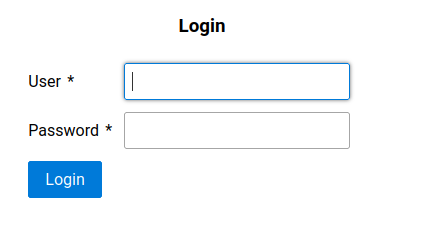
\includegraphics[width=0.40\textwidth]{imaxes/login.png}
  \caption{Pantalla de logado}
  \label{fig:login}
\end{figure}

Si los datos introducidos son correctos se mostrará la página de inicio de la aplicación.

Para salir de la aplicación pulsaremos el botón con nuestro nombre de usuario situado en la esquina superior derecha y seleccionaremos la opción logout (ver \figurename~\ref{fig:logout}). Una vez pulsado se cierra la sesión y la aplicación nos redirige a la pantalla de inicio de sesión.

\begin{figure}[H]
  \centering
  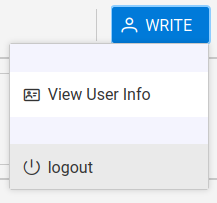
\includegraphics[width=0.25\textwidth]{imaxes/logout.png}
  \caption{Logout}
  \label{fig:logout}
\end{figure}


\subsection{Cambio de contraseña y/o datos de contacto de un usuario}
\label{sub:contraseña}
Un usuario puede modificar tanto su contraseña de acceso como los datos relativos a su ficha. Para ello pulsará el botón de la esquina superior derecha con su nombre de usuario y seleccionará la opción \textit{View User Info} .
Se mostrará una pantalla con un botón para cambiar la contraseña así como un área con los datos del usuario y un botón para editar la información.

\begin{description}
\item[\underline{\textsl{Modificar contraseña}}] Se pulsará el botón \emph{Change Password}. Aparecerán dos campos editables para introducir la nueva contraseña a cambiar y un botón para guardar los cambios. Los valores introducidos en ambos campos deberán ser iguales. En caso contrario la aplicación mostrará un error de validación y no se modificará la contraseña.

\item[\underline{\textsl{Editar información del usuario}}] Pulsando el botón \emph{Edit Data} se habilitará la edición de los campos con la información del usuario y un botón para guardar los cambios.
\end{description}


\subsection{Acceder al menú de la aplicación}
\label{sub:menu}
Pulsando el botón \emph{Menu} de la esquina superior izquierda se despliega el menú de la aplicación (\figurename~\ref{fig:menu}).

\begin{figure}[H]
  \centering
  
\includegraphics[width=0.6\textwidth]{imaxes/menu-aplicacion.png}
  \caption{Detalle del menú de la aplicación}
  \label{fig:menu}
\end{figure}

El menú se divide en cuatro bloques:
\begin{itemize}
\item \emph{\textbf{PARAMETERS}}: da acceso a las distintas entidades de parametrización, necesarias para la definición del resto de entidades de la aplicación.
\item \emph{\textbf{CATALOG}}: da acceso a las distintas entidades del catálogo de servicios de la aplicación.
\item \emph{\textbf{CONTRACT}}: da acceso a las distintas entidades de contratación de la aplicación.
\item \emph{\textbf{HIERARCHY}}: da acceso a la ventana de visualización jerárquica de las contrataciones.
\end{itemize}

El botón que se encuentra más a la izquierda, fuera del área del menú, permite ocultar la ventana emergente del menú.


A continuación entraremos en detalle en cada uno de estos apartados.

\subsection{Parametrización}
\label{sub:parametrizacion}

Con idea de hacer lo más flexible y adaptable posible esta aplicación, se han definido una serie de elementos de parametrización para la definición de las distintas entidades de la aplicación. En la \tablename~\ref{tab:parametrizacion} se puede consultar un listado de los elementos de parametrización existentes en la aplicación. Para acceder a cada una de estas entidades se desplegará la sección \emph{PARAMETERS} del menú principal y se seleccionará el tipo de entidad correspondiente del listado desplegado.



\begin{table}[H]
  \centering
  \rowcolors{2}{white}{udcgray!25}
  \setlength{\leftmargini}{0.4cm}
  \resizebox{14cm}{!} {
  \begin{tabular}{|m{4cm} m{11cm}|}
  \rowcolor{udcpink!25}
  \hline
  	\textbf{Elemento} & \textbf{Descripción} \\\hline
	\textbf{Entity Types} & Listado de entidades contempladas en el sistema. Son siete, correspondientes a producto, servicio, cuota, consumo, promoción, cliente y cuenta.   \\
	\textbf{Consumption Classes} & Clases de consumos definidos. Actualmente hay cuatro correspondientes a llamada, SMS, MMS y Datos. Necesario para definir los consumos definidos en el catálogo. \\
	\textbf{Status} & Estados permitidos dentro del sistema para las entidades del catálogo y la contratación.. Se definen dos ámbitos de aplicación: para las entidades del catálogo y/o para las de la contratación. Un mismo estado puede ser compartido por entidades de distinto ámbito. \\
	\textbf{Application Level} & Define el nivel de aplicación de las cuotas y las promociones. Actualmente hay dos niveles definidos: producto y servicio.  \\
	\textbf{Discount Type} & Tipos de descuento existentes en la aplicación. Usados para definir las promociones. Actualmente hay cuatro tipos: (volumen de) Megabytes, (volumen de) minutos, unidades (número de sms) y porcentaje (a descontar sobre el total facturado).   \\
	\textbf{Payment Method} & Métodos de pago. Se usa a la hora de instanciar una cuenta (contratación) para definir el método de pago de ese cliente. \\
Billing Period & Los distintos períodos de facturación definidos. Usado para definir los distintos tipos de facturación. \\
	\textbf{Tax Type} & Tipo impositivo. Usado durante la contratación de un producto o servicio, para definir el tipo impositivo que se debe aplicar sobre el mismo de cara a la facturación.\\
	\textbf{Identity Card Type} & Tipo de documento de identificación (NIF, NIE, Pasaporte).
	\\\hline
  \end{tabular}
  } % end /resizebox
  \caption{Entidades de Parametrización}
  \label{tab:parametrizacion}
\end{table}

La gestión de estas entidades no está disponible para todos los usuarios, tal y como se muestra en la \figurename~\ref{fig:parametrizacion}). Sólo los usuarios con permisos de administrador de la aplicación podrán añadir, editar o borrar elementos, habilitándoseles los correspondientes botones para dichas operaciones (\figurename~\ref{fig:parametrizacion-admin}). Para el resto de usuarios sólo se mostrará el listado de dichos elementos (\figurename~\ref{fig:parametrizacion-usuario}).


\begin{figure}[H]
  \centering
  \begin{subfigure}[c]{\textwidth}
    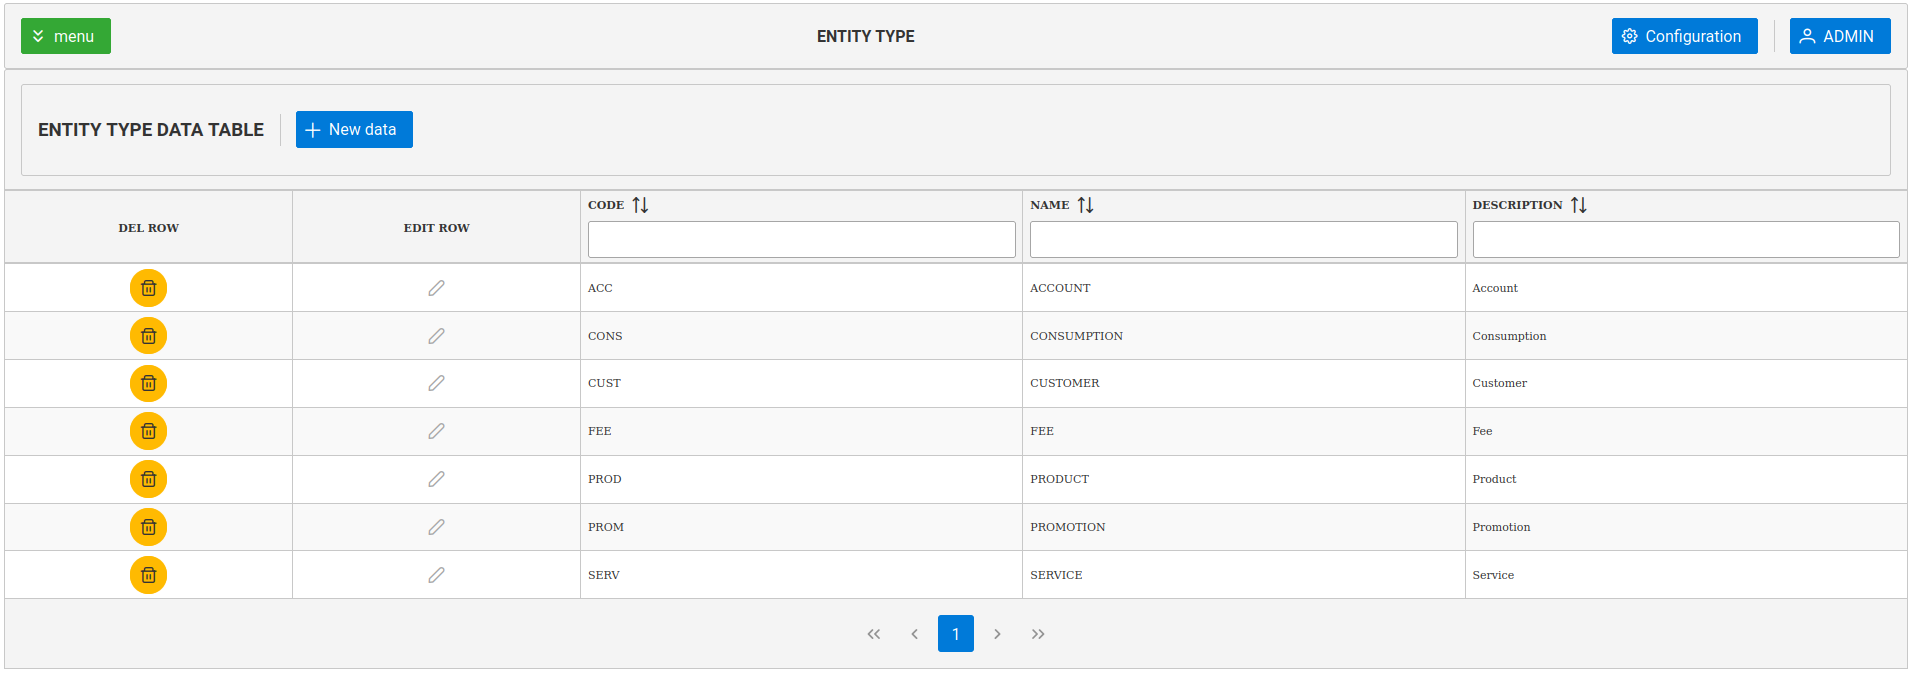
\includegraphics[width=\textwidth]{imaxes/entity-type-admin.png}
    \caption{Vista de la pantalla Entity Types para usuarios con perfil de administrador\newline}
    \label{fig:parametrizacion-admin}
  \end{subfigure}
  \begin{subfigure}[c]{\textwidth}
    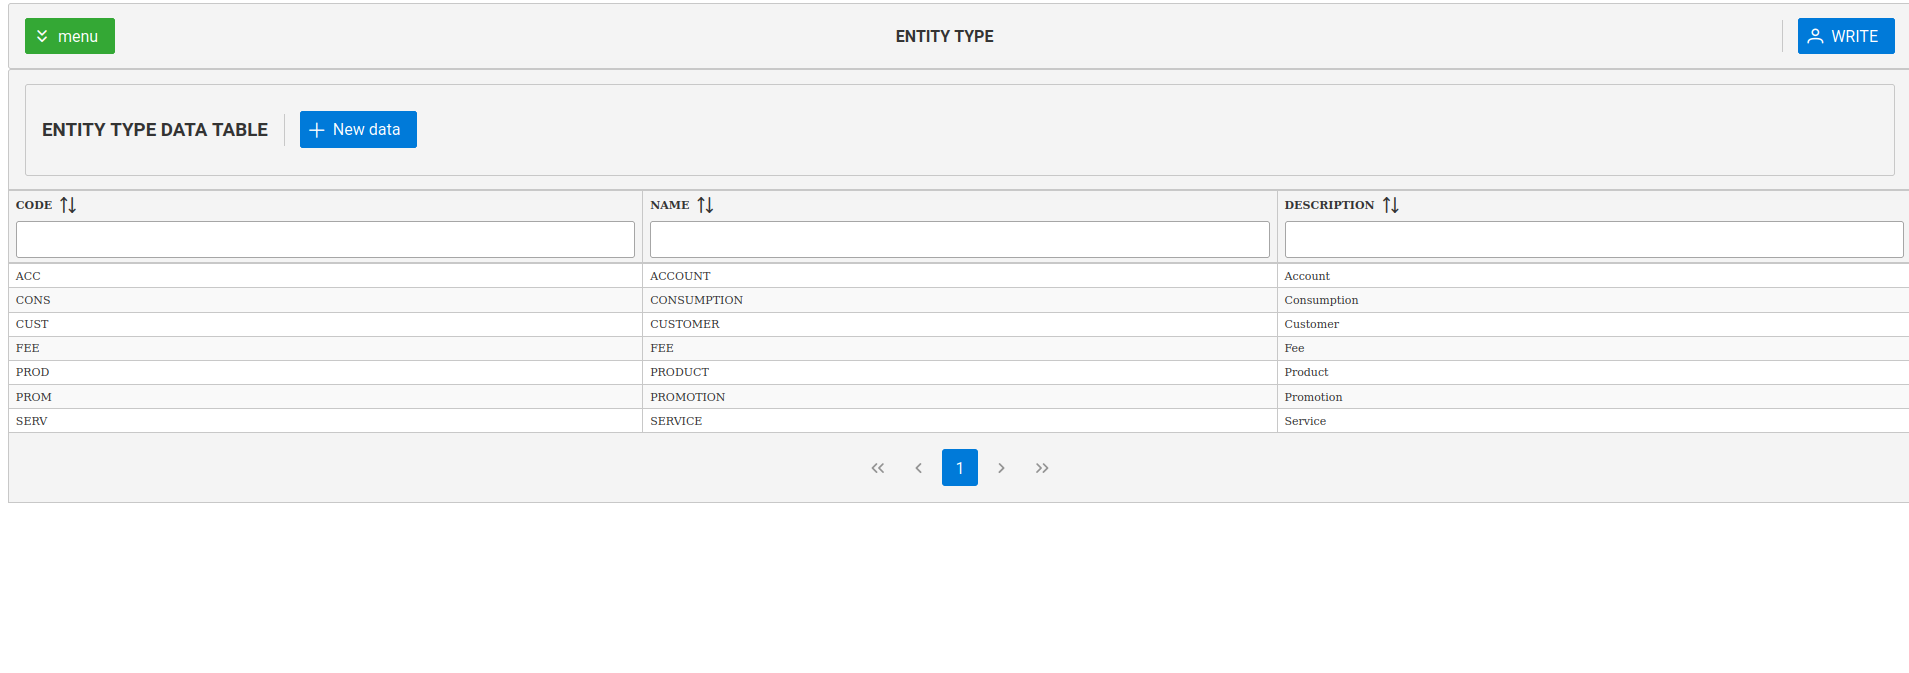
\includegraphics[width=\textwidth,height=3cm]{imaxes/entity-type-usuario.png}
    \caption{Vista de la pantalla Entity Types para el resto de perfiles de usuario}
    \label{fig:parametrizacion-usuario}
  \end{subfigure}
  \caption{Comparativa de las vistas de la pantalla Entity Types según los permisos del usuario.}
  \label{fig:parametrizacion}
\end{figure}

Para los usuarios con perfil de administrador se definen las siguientes operaciones, siendo \textit{entidad} el tipo de elemento al que hemos accedido a través del menú. El funcionamiento es el mismo para todas las entidades, sólo cambia la información a almacenar, que vendrá dada por la naturaleza de la misma.

\begin{description}
\item[\underline{\textsl{\textbf{Crear nueva entidad}}}] Para crear una nueva entidad se pulsará el botón \textit{New Data} situado en la parte superior de la tabla. Aparecerá una ventana emergente que mostrará un formulario con los campos a cubrir.

\item[\underline{\textsl{\textbf{Editar entidad existente}}}] Para editar una entidad se seleccionará del listado y se pulsará el botón editar de la columna \textit{EDIT ROW} correspondiente. Se editarán los campos pertinentes directamente en la tabla para realizar las modificaciones oportunas. 

\item[\underline{\textsl{\textbf{Borrar entidad}}}] Para borrar una entidad se seleccionará del listado y se pulsará el botón amarillo de borrar de la columna \textit{DEL ROW} correspondiente.
\end{description}

Todos los valores mostrados para la entidad son obligatorios y deberán cubrirse al realizar un alta o modificación. Asimismo el valor del campo CODE es único. No pueden existir dos entidades del mismo tipo con el mismo código.


\subsection{Catálogo}
\label{sub:catálogo}

El catálogo del sistema está formado por las distintas definiciones de productos, servicios, cuotas, consumos y promociones que ofrece la empresa y las relaciones que guardan entre sí. A estas definiciones les hemos dado en llamar tipos (\textit{type}).

Además de estas seis entidades indicadas, hemos incluido en esta clasificación otras entidades, que si bien no forman parte del catálogo de servicios de una empresa propiamente dicho, sí son definiciones de entidades que nos ayudarán a clasificar los datos a la hora de realizar contrataciones.


Todos los usuarios del sistema tienen acceso a los elementos del catálogo, pero aquellos que tengan permisos de edición (perfil ADMIN o MODIF) podrán gestionarlos (realizar altas, bajas y modificaciones). Los usuarios con el perfil READ sólo podrán acceder en modo consulta, y no se mostrarán habilitados los correspondientes botones para las operaciones de gestión. Por comodidad las imágenes que proceden a ilustrar esta sección se corresponderán con el acceso a las vistas de un usuario con permisos de edición. Los usuarios sin estos permisos verán la misma pantalla pero sin los botones que permiten la gestión de los datos.


Se definen tres estados distintos para las entidades del catálogo:
\begin{description}
\item[ACTIVE] Estado activo. Para las entidades del catálogo que están disponibles para ofertar.
\item[DEVELOP] Estado \textit{en desarrollo}. Para las entidades del catálogo que todavía no están disponibles para ofertar.
\item[CANCEL] Estado cancelado. Para las entidades del catálogo que están disponibles para ofertar.
\end{description}



A continuación detallaremos cada una de estas entidades a las que accederemos a través del menú \emph{CATALOG}.

\subsubsection{Bill Cycle Type - Tipo de ciclo de facturación}
\label{sub:billcycle}

Nota: Para acceder a la pantalla que da acceso a la operativa de este tipo de entidad se desplegará la sección \emph{CATALOG} del menú principal y se seleccionará el tipo de entidad \emph{Bill Cycle Type}.

La facturación escapa del ámbito de esta aplicación. Sin embargo toda contratación de servicios tiene como fin último monetizar la prestación de un servicio, por lo que la información del ciclo de facturación en el que va a entrar un elemento contratado es un factor a tener en cuenta a la hora de de realizar las contrataciones.

Un tipo de ciclo de facturación viene definido por los elementos indicados en la \tablename~\ref{tab:ciclo-facturacion}:



\begin{table}[H]
  \centering
  \rowcolors{2}{white}{udcgray!25}
  \setlength{\leftmargini}{0.4cm}
  \resizebox{14cm}{!} {
  \begin{tabular}{|m{3.5cm} m{11cm}|}
  \rowcolor{udcpink!25}
  \hline
  	\textbf{Elemento} & \textbf{Descripción} \\\hline
	\textbf{CODE} & Código identificativo del ciclo de facturación. Es único.   \\
	\textbf{NAME} & Nombre del ciclo del facturador. \\
	\textbf{DESCRIPTION} & Descripción del ciclo de facturador. \\
	\textbf{CORRECTIVE} & Valor \emph{True} indica que estamos ante un ciclo de facturación correctivo (a aplicar en refacturaciones). En caso contrario estaremos ante un ciclo de facturación ordinario (el que se ejecuta periódicamente)\\
	\textbf{BILLING PERIOD} & Período de facturación definido para el ciclo de facturación. Se corresponde con los períodos de facturación definidos en la correspondiente entidad de \emph{PARAMETERS} definida en la sección \ref{sub:parametrizacion}.   \\
	\textbf{BILL CYCLE DAY} & Día en el que se inicia un período de facturación. \\
	\textbf{CODENUM} & Código alfanumérico que identifica el número de la factura.\\
	\textbf{STATUS} & Estado del ciclo de facturación.
	\\\hline
  \end{tabular}
  } % end /resizebox
  \caption{Datos que definen el ciclo de facturación.}
  \label{tab:ciclo-facturacion}
\end{table}


Las operaciones definidas para esta entidad son las siguientes (nota: sólo están habilitadas para usuarios con permisos de edición):
\begin{description}
  \item[\underline{\textsl{\textbf{Crear nuevo tipo de ciclo de facturación}}}] Para crear un nuevo tipo ciclo de facturación se pulsará el botón \textit{New Data} situado en la parte superior de la tabla. Aparecerá una ventana emergente que mostrará un formulario con los campos a cubrir.

  \item[\underline{\textsl{\textbf{Editar tipo de ciclo de facturación existente}}}] Para editar un tipo de ciclo de facturación existente se seleccionará del listado y se pulsará el botón editar de la columna \textit{EDIT ROW} correspondiente. Se editarán los campos pertinentes directamente en la tabla para realizar las modificaciones oportunas. 

  \item[\underline{\textsl{\textbf{Borrar ciclo de facturación}}}] Para borrar un tipo de ciclo de facturación se seleccionará del listado y se pulsará el botón amarillo de borrar de la columna \textit{DEL ROW} correspondiente.
\end{description}

Todos los valores mostrados para la entidad son obligatorios y deberán cubrirse al realizar un alta o modificación. Asimismo el valor del campo CODE es único. No pueden existir dos entidades del mismo tipo con el mismo código.



\subsubsection{Customer Type - Tipo de cliente}
\label{sub:customer-type}

Nota: Para acceder a la pantalla que da acceso a la operativa de este tipo de entidad se desplegará la sección \emph{CATALOG} del menú principal y se seleccionará el tipo de entidad \emph{Customer Type}.

En este apartado nos centraremos en la gestión de los tipos de cliente, que permiten clasificar los distintos clientes de la cartera de clientes existentes en el sistema.


Un tipo de cliente viene definido por los elementos indicados en la \tablename~\ref{tab:tipo-cliente}:



\begin{table}[H]
  \centering
  \rowcolors{2}{white}{udcgray!25}
  \setlength{\leftmargini}{0.4cm}
  \resizebox{14cm}{!} {
  \begin{tabular}{|m{3cm} m{11cm}|}
  \rowcolor{udcpink!25}
  \hline
  	\textbf{Elemento} & \textbf{Descripción} \\\hline
	\textbf{CODE} & Código identificativo del tipo del cliente. Es único.   \\
	\textbf{NAME} & Nombre del tipo del cliente. \\
	\textbf{DESCRIPTION} & Descripción del tipo de cliente. \\	
	\textbf{STATUS} & Estado del tipo de cliente.
	\\\hline
  \end{tabular}
  } % end /resizebox
  \caption{Datos que define un tipo de cliente.}
  \label{tab:tipo-cliente}
\end{table}

Las operaciones definidas para esta entidad son las siguientes (nota: sólo están habilitadas para usuarios con permisos de edición):
\begin{description}
\item[\underline{\textsl{\textbf{Crear nuevo tipo de cliente}}}] Para crear un nuevo cliente se pulsará el botón \textit{New Data} situado en la parte superior de la tabla. Aparecerá una ventana emergente que mostrará un formulario con los campos a cubrir.

\item[\underline{\textsl{\textbf{Editar tipo de cliente existente}}}] Para editar un tipo de cliente existente se seleccionará del listado y se pulsará el botón editar de la columna \textit{EDIT ROW} correspondiente. Se editarán los campos pertinentes directamente en la tabla para realizar las modificaciones oportunas. 

\item[\underline{\textsl{\textbf{Borrar tipo de cliente}}}] Para borrar un tipo de cliente se seleccionará del listado y se pulsará el botón amarillo de borrar de la columna \textit{DEL ROW} correspondiente.
\end{description}

Todos los valores mostrados para la entidad son obligatorios y deberán cubrirse al realizar un alta o modificación. Asimismo el valor del campo CODE es único. No pueden existir dos entidades del mismo tipo con el mismo código.




\subsubsection{Account Type - tipo de cuenta}
\label{sub:account-type}

Nota: Para acceder a la pantalla que da acceso a la operativa de este tipo de entidad se desplegará la sección \emph{CATALOG} del menú principal y se seleccionará el tipo de entidad \emph{Customer Type}.

En este apartado nos centraremos en la gestión de los tipos de cuenta, que permiten clasificar las distintas cuentas de la cartera de clientes existentes en el sistema.

Una cuenta es la entidad que alberga el conjunto de elementos contratados y es sobre la que se definen los datos de facturación. Un cliente puede tener varias cuentas en función de, por ejemplo, la ubicación en la que se encuentran los servicios contratados (por ejemplo una cuenta para la vivienda habitual y otra para la segunda residencia). 


Un tipo de cuenta viene definido por los elementos indicados en la \tablename~\ref{tab:tipo-cuenta}:



\begin{table}[H]
  \centering
  \rowcolors{2}{white}{udcgray!25}
  \setlength{\leftmargini}{0.4cm}
  \resizebox{14cm}{!} {
  \begin{tabular}{|m{4cm} m{11cm}|}
  \rowcolor{udcpink!25}
  \hline
  	\textbf{Elemento} & \textbf{Descripción} \\\hline
	\textbf{CODE} & Código identificativo del tipo de cuenta. Es único.   \\
	\textbf{NAME} & Nombre del tipo de cuenta. \\
	\textbf{DESCRIPTION} & Descripción del tipo de cuenta. \\	
	\textbf{PAYMENT METHOD} & Tipo de pago asociado a la cuenta. Se corresponde con los métodos de pago definidos en la correspondiente entidad de \emph{PARAMETERS} definida en la sección \ref{sub:parametrizacion}. \\	
	\textbf{ORDINARY CYCLE} & Tipo de ciclo de facturación ordinario especificado para este tipo de cuenta. Se corresponde los tipos de ciclo de facturación definidos como ordinarios de la entidad de catálogo \ref{sub:billcycle}. \\	 		\textbf{CORRECTIVE CYCLE} & Tipo de ciclo de facturación correctivo especificado para este tipo de cuenta. Se corresponde los tipos de ciclo de facturación definidos como correctivos de la entidad de catálogo \ref{sub:billcycle}. \\	
	\textbf{STATUS} & Estado del tipo de la cuenta.
	\\\hline
  \end{tabular}
  } % end /resizebox
  \caption{Datos que define un tipo de cuenta.}
  \label{tab:tipo-cuenta}
\end{table}

Las operaciones definidas para esta entidad son las siguientes (nota: sólo están habilitadas para usuarios con permisos de edición):
\begin{description}
\item[\underline{\textsl{\textbf{Crear nuevo tipo de cuenta}}}] Para crear una nueva cuenta se pulsará el botón \textit{New Data} situado en la parte superior de la tabla. Aparecerá una ventana emergente que mostrará un formulario con los campos a cubrir.

\item[\underline{\textsl{\textbf{Editar tipo de cuenta existente}}}] Para editar un tipo de cuenta existente se seleccionará del listado y se pulsará el botón editar de la columna \textit{EDIT ROW} correspondiente. Se editarán los campos pertinentes directamente en la tabla para realizar las modificaciones oportunas.

\item[\underline{\textsl{\textbf{Borrar tipo de cuenta}}}] Para borrar un tipo de cuenta se seleccionará del listado y se pulsará el botón amarillo de borrar de la columna \textit{DEL ROW} correspondiente.
\end{description}

Todos los valores mostrados para la entidad son obligatorios y deberán cubrirse al realizar un alta o modificación. Asimismo el valor del campo CODE es único. No pueden existir dos entidades del mismo tipo con el mismo código.




\subsubsection{Consumption Type - tipo de consumo}
\label{sub:consumption-type}

Nota: Para acceder a la pantalla que da acceso a la operativa de este tipo de entidad se desplegará la sección \emph{CATALOG} del menú principal y se seleccionará el tipo de entidad \emph{Consumption Type}.

Consideramos los tipos de consumo como entidades perteneciente al catálogo de servicios propiamente dicho.

Como ya hemos indicado anteriormente, el importe a facturar por los consumos no puede saberse de antemano, ya que va ligada a los comportamientos a la hora de consumir esos elementos facturables. Sin embargo, puesto que como todo elemento facturable es susceptible de ser descontado por una promoción, deberemos guarda la definición de estos consumos.

Para simplificar su manejo nos hemos quedado con una definición lo más simple posible de este tipo de elementos facturables para poder establecer una relación entre estos elementos y los posibles descuentos a aplicar sobre los mismos. Por lo tanto se ignora lo relativo la información relativa a los costes asociados a los mismos, ya que esto está ligado a la definición de la tarificación de estos elementos facturables y consideramos que entra dentro del ámbito de un sistema de tarificación. 

Un tipo de consumo viene definido por los elementos indicados en la \tablename~\ref{tab:tipo-consumo}:



\begin{table}[H]
  \centering
  \rowcolors{2}{white}{udcgray!25}
  \setlength{\leftmargini}{0.4cm}
  \resizebox{14cm}{!} {
  \begin{tabular}{|m{3cm} m{11cm}|}
  \rowcolor{udcpink!25}
  \hline
  	\textbf{Elemento} & \textbf{Descripción} \\\hline
  	\textbf{CONSUMPTION CLASS} & Clase de consumo que estamos tratando. Las clases de consumo están definidas en la correspondiente entidad de \emph{PARAMETERS} definida en la sección \ref{sub:parametrizacion}.   \\
	\textbf{CODE} & Código identificativo del tipo de consumo. Es único.   \\
	\textbf{NAME} & Nombre del tipo de consumo. \\
	\textbf{DESCRIPTION} & Descripción del tipo de consumo. \\		
	\textbf{STATUS} & Estado del tipo del consumo.
	\\\hline
  \end{tabular}
  } % end /resizebox
  \caption{Datos que define un tipo de consumo.}
  \label{tab:tipo-consumo}
\end{table}

Las operaciones definidas para esta entidad son las siguientes (nota: sólo están habilitadas para usuarios con permisos de edición):
\begin{description}
\item[\underline{\textsl{\textbf{Crear nuevo tipo de consumo}}}] Para crear un nuevo consumo se pulsará el botón \textit{New Data} situado en la parte superior de la tabla. Aparecerá una ventana emergente que mostrará un formulario con los campos a cubrir.

\item[\underline{\textsl{\textbf{Editar tipo de consumo existente}}}] Para editar un tipo de consumo existente se seleccionará del listado y se pulsará el botón editar de la columna \textit{EDIT ROW} correspondiente. Se editarán los campos pertinentes directamente en la tabla para realizar las modificaciones oportunas.

\item[\underline{\textsl{\textbf{Borrar tipo de consumo}}}] Para borrar un tipo de consumo se seleccionará del listado y se pulsará el botón amarillo de borrar de la columna \textit{DEL ROW} correspondiente.
\end{description}

Todos los valores mostrados para la entidad son obligatorios y deberán cubrirse al realizar un alta o modificación. Asimismo el valor del campo CODE es único. No pueden existir dos entidades del mismo tipo con el mismo código.





\subsubsection{Fee Types - tipo de cuota}
\label{sub:fee-type}

Nota: Para acceder a la pantalla que da acceso a la operativa de este tipo de entidad se desplegará la sección \emph{CATALOG} del menú principal y se seleccionará el tipo de entidad \emph{Fee Types}.

Consideramos los tipos de cuotas como entidades pertenecientes al catálogo de servicios propiamente dicho.

A diferencia de los consumos, los cargos a facturar generados por las cuotas sí son conocidos de antemano y se definen dentro del catálogo de servicio.

Puesto que el importe de los cargos a facturar generados por las cuotas varían con el tiempo, se ha considerado la necesidad de llevar un registro de estos cambios a lo largo de la vida útil de este tipo de elementos. Por lo tanto una entidad de este tipo estará conformada por uno o varios registros con una fecha inicio y una fecha fin que definen el período en el que aplican las condiciones definidas para esa entidad. Estos registros deben ser consecutivos de forma que si existen varios registros la fecha de inicio de un registro debe ser la fecha de fin del registro anterior mas un día (salvo para el primer registro que conforma el período del ciclo de vida del elemento). De igual forma la fecha de finalización de un registro debe ser la fecha de inicio del registro siguiente menos un día (salvo para el último registro que conforma el período del ciclo de vida del elemento).


Un tipo de cuota viene definido por los elementos indicados en la \tablename~\ref{tab:tipo-cuota}:




\begin{table}[H]
  \centering
  \rowcolors{2}{white}{udcgray!25}
  \setlength{\leftmargini}{0.4cm}
  \resizebox{14cm}{!} {
  \begin{tabular}{|m{3cm} m{11cm}|}
  \rowcolor{udcpink!25}
  \hline
  	\textbf{Elemento} & \textbf{Descripción} \\\hline
  	\textbf{START DATE} & Fecha de inicio del período temporal para el que aplican las condiciones especificadas para dicho período.\\
  	\textbf{END DATE} & Fecha de finalización del período temporal para el que aplican las condiciones especificadas para dicho período.\\
  	\textbf{CODE} & Código identificativo del tipo de cuota. Es único.\\
	\textbf{NAME} & Nombre del tipo de cuota.\\
	\textbf{DESCRIPTION} & Descripción del tipo de cuota.\\
	\textbf{APPLICATION LEVEL} & Nivel de aplicación de la cuota, esto es, a qué entidad facturable va asociado. Los niveles de aplicación están definidas en la correspondiente entidad de \emph{PARAMETERS} definida en la sección \ref{sub:parametrizacion}.\\	
	\textbf{PRORRATE} & Indica si la cuota es prorrateable (\textit{TRUE}) o no (\textit{FALSE}).\\
	\textbf{PRICE} & Indica el importe a facturar por dicha cuota.\\
	\textbf{STATUS} & Estado del tipo de cuota.	
	\\\hline
  \end{tabular}
  } % end /resizebox
  \caption{Datos que define un tipo de cuota.}
  \label{tab:tipo-cuota}
\end{table}



Las operaciones definidas para esta entidad son las siguientes:
\begin{description}
\item[\underline{\textsl{\textbf{Buscar un tipo de cuota existente}}}] Esta operación está disponible para todos los usuarios de la aplicación.

Puesto que los tipos de cuota son entidades con histórico, por motivos de operatividad no se muestra el listado de todas las entidades del sistema por defecto, si no que se establecen unos criterios de búsqueda para seleccionar el tipo de cuota a consultar. Para ello se define un área de búsqueda en los que se definen los criterios de búsqueda a tener en cuenta:
\begin{itemize}
\item Buscar todos los históricos de los tipos de consumo. Se realizará una búsqueda de todos los históricos de los distintos tipos de consumo.
\item Buscar por fecha. Se realizará una búsqueda de los históricos de todos los tipos de consumo existentes en el sistema para los que la fecha de búsqueda definida se encuentre entre la fecha de inicio y fin del registro de histórico. Opción marcada por defecto
\end{itemize}

Pulsando el botón \emph{Search} se mostrará un panel emergente con el listado de los registros encontrados. Seleccionaremos el elemento sobre el que queramos operar pulsando el botón amarillo de la columna \emph{Show Historic} (\figurename~\ref{fig:seleccion-tipo-cuota}):

\begin{figure}[H]
  \centering
  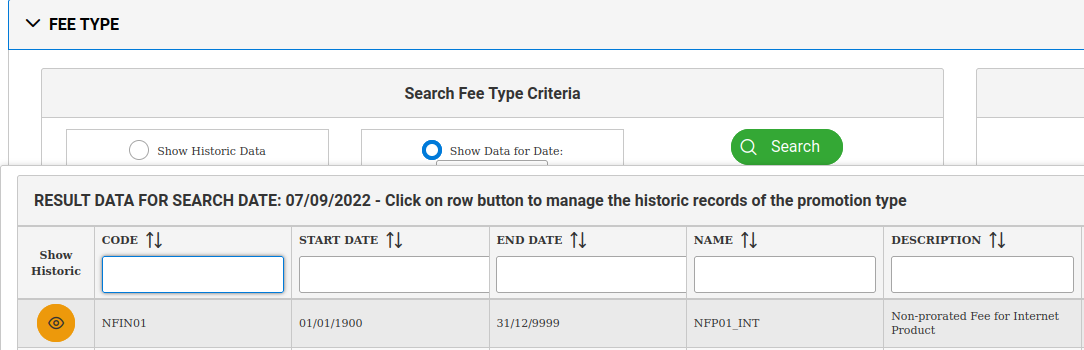
\includegraphics[width=0.90\textwidth]{imaxes/seleccion-tipo-cuota.png}
  \caption{Selección del tipo de cuota a modificar}
  \label{fig:seleccion-tipo-cuota}
\end{figure}


Se mostrará el área de históricos de la entidad con los distintos registros de histórico existentes (\figurename~\ref{fig:listado-historicos-tipo-cuota}):

\begin{figure}[H]
  \centering
  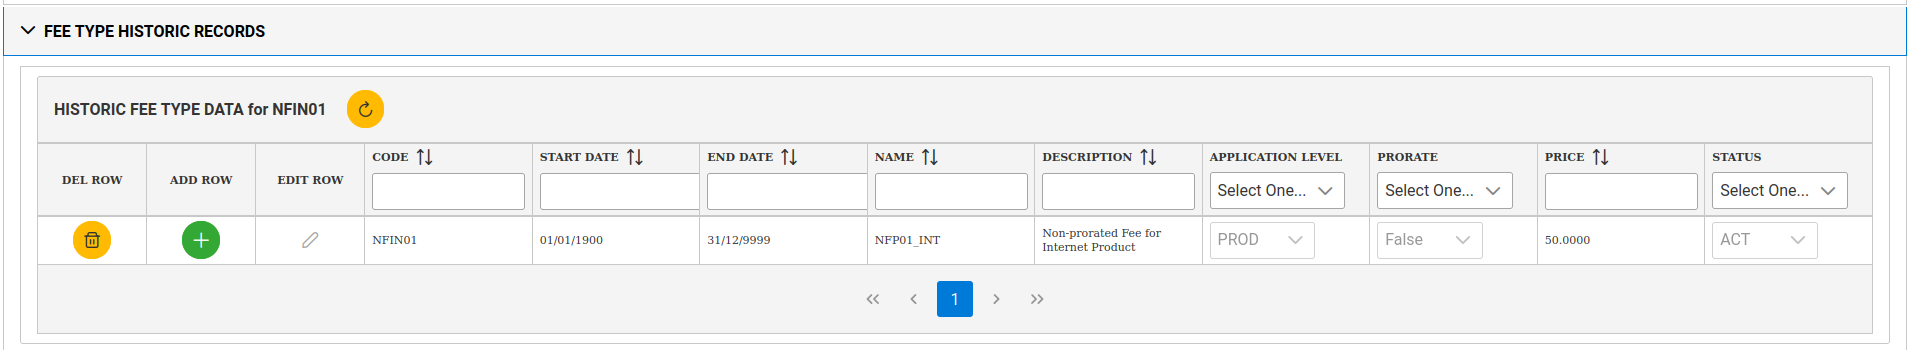
\includegraphics[width=\textwidth]{imaxes/listado-historicos-tipo-cuota.png}
  \caption{Listado de los históricos del tipo de cuota}
  \label{fig:listado-historicos-tipo-cuota}
\end{figure}


\item[\underline{\textsl{\textbf{Crear nuevo tipo de cuota}}}] Esta operación sólo está habilitada para usuarios con permisos de edición.
Para crear un nuevo consumo se pulsará el botón \textit{New Data} situado en la parte superior de la tabla. Aparecerá una ventana emergente que mostrará un formulario con los campos a cubrir. Por defecto se establecen como fecha de inicio y fin del nuevo tipo de cuota las fechas 01/01/1900 y 31/12/9999.

\item[\underline{\textsl{\textbf{Editar registro de histórico de un tipo de cuota existente}}}] Esta operación sólo está disponible para usuarios con permisos de edición.
Para editar un tipo de consumo existente se seleccionará del listado y se pulsará el botón editar de la columna \textit{EDIT ROW} correspondiente. Se editarán los campos pertinentes directamente en la tabla para realizar las modificaciones oportunas teniendo en cuenta los criterios de fechas establecidos (definidos en la sección \ref{sub:histórico-conceptos} de la página \pageref{sub:histórico-conceptos}).

\item[\underline{\textsl{\textbf{Añadir registro de histórico de un tipo de cuota existente}}}] Esta operación sólo está disponible para usuarios con permisos de edición.
Para añadir un nuevo registro de histórico sobre tipo de consumo existente se seleccionará del listado el registro en el que se ubicará el nuevo registro a añadir 
y se pulsará el botón añadir de la columna \textit{ADD ROW} correspondiente. Aparecerá una nueva ventana emergente como la que se muestra en la operación de creación, pero con los campos cubiertos con la información del registro sobre el que se va a añadir el nuevo registro y se realizarán las modificaciones oportunas teniendo en cuenta los criterios de fechas establecidos (definidos en la sección \ref{sub:histórico-conceptos} de la página \pageref{sub:histórico-conceptos}).

\item[\underline{\textsl{\textbf{Borrar registro de histórico del tipo de cuota}}}] Esta operación sólo está disponible para usuarios con permisos de edición.
Para borrar un registro de histórico del tipo de consumo se seleccionará del listado el registro a borrar y se pulsará el botón amarillo de borrar de la columna \textit{DEL ROW} correspondiente.

\item[\underline{\textsl{\textbf{Borrar el tipo de cuota}}}] Esta operación sólo está disponible para usuarios con permisos de edición.
Para borrar completamente un tipo de cuota se deben borrar uno a uno todos los registros de histórico del tipo de cuota según lo indicado en el punto anterior. 

Todos los valores mostrados para la entidad son obligatorios y deberán cubrirse al realizar un alta o modificación. Asimismo el valor del campo CODE es único. No pueden existir dos entidades del mismo tipo con el mismo código.
\end{description}

A continuación describimos cómo proceder para realizar las distintas operaciones de modificación de un registro de histórico (edición de registro de histórico, añadir un nuevo registro de histórico y borrar un registro de histórico). Como paso previo a estas operaciones deberemos haber buscado la entidad de tipo cuota a modificar:


\paragraph{Añadir un nuevo registro de histórico:} para ello seleccionamos el registro de histórico a modificar y pulsamos el botón verde \emph{ADD ROW}. Aparecerá una ventana emergente con un formulario de edición. Modificamos los datos correspondientes, por ejemplo la fecha inicio del nuevo registro y el importe de la cuota y pulsamos el botón azul \emph{OK} de confirmación (\figurename~\ref{fig:añadir-registro-historico-tipo-cuota}).

\begin{figure}
  \centering
  \includegraphics[width=0.45\textwidth]{imaxes/añadir-registro-historico-tipo-cuota.png}
  \caption{Formulario para añadir un nuevo registro de histórico del tipo de cuota}
  \label{fig:añadir-registro-historico-tipo-cuota}
\end{figure}


Una vez pulsado el botón de confirmación se cierra el formulario y se muestra la lista actualizada del registro de histórico con la nueva definición del tipo de consumo. Comprobamos que se ha modificado la fecha de inicio del registro ya existente en el sistema y que figura el nuevo registro añadido con los correspondientes valores modificados, tal y como se muestra en la \figurename~\ref{fig:listado-historico-tipo-consumo-tras-añadir}.

\begin{figure}
  \centering
  \includegraphics[width=\textwidth]{imaxes/listado-historico-tipo-consumo-tras-añadir.png}
  \caption{Listado de registros de histórico tras la adición de un nuevo registro de histórico}
  \label{fig:listado-historico-tipo-consumo-tras-añadir}
\end{figure}


\paragraph{Borrar un registro de histórico:} para ello seleccionamos el registro de histórico a modificar y pulsamos el botón amarillo \emph{DEL ROW}, por ejemplo el registro añadido en el ejemplo anterior. Aparecerá un diálogo de confirmación indicando el período del registro a borrar, tal y como se muestra en la \figurename~\ref{fig:borrado-historico-tipo-cuota}.


\begin{figure}
  \centering
  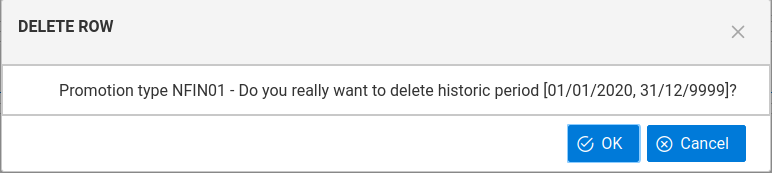
\includegraphics[width=0.70\textwidth]{imaxes/borrado-historico-tipo-cuota.png}
  \caption{Diálogo de confirmación del borrado del registro de histórico seleccionado}
  \label{fig:borrado-historico-tipo-cuota}
\end{figure}


Una vez pulsado el botón  \emph{OK}  de confirmación de la operación se cerrará el cuadro de diálogo y se mostrará el listado de históricos de la entidad actualizado tal y como muestra la \figurename~\ref{fig:listado-historico-tipo-consumo-tras-borrar}.


\begin{figure}
  \centering
  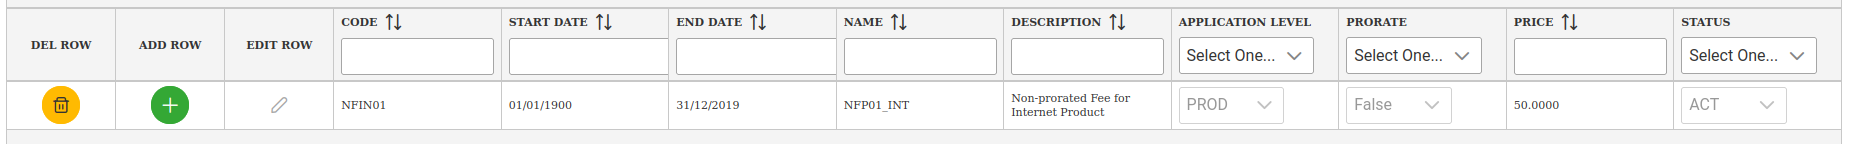
\includegraphics[width=\textwidth]{imaxes/listado-historico-tipo-consumo-tras-borrar.png}
  \caption{Listado de registros de histórico tras el borrado de un registro de histórico}
  \label{fig:listado-historico-tipo-consumo-tras-borrar}
\end{figure}




\paragraph{Editar un registro de histórico:} para ello seleccionamos el registro de histórico a editar y pulsamos el botón de edición de la columna \emph{EDIT ROW}. El registro del diálogo muestra los campos susceptibles de modificarse como editables, pudiendo realizar las modificaciones oportunas en el registro del listado. En caso de modificar el campo \emph{STATUS} del registro a \emph{CANCEL} se mostrará un cuadro de diálogo solicitando confirmación de extender este estado a todos los registros de histórico posteriores al actual, ya que se considera que una vez cancelado un registro todos los registros posteriores deben compartir dicho estado.

Supongamos el siguiente ejemplo que se ve en la \figurename~\ref{fig:listado-tipos-cuotas-inicial}: un tipo de consumo con varios registros de histórico, al que vamos a cambiar el estado del segundo registro de histórico a \emph{CANCEL}.

\begin{figure}[H]
  \centering
  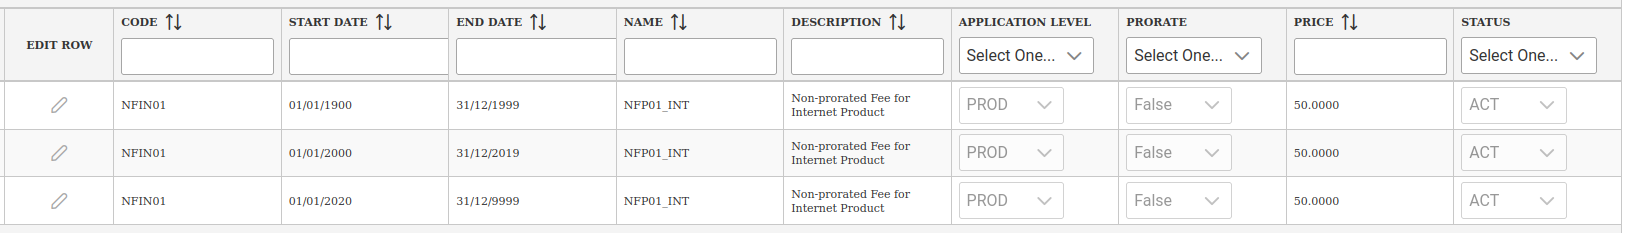
\includegraphics[width=\textwidth]{imaxes/listado-tipos-cuotas-inicial.png}
  \caption{Listado inicial de registros de histórico}
  \label{fig:listado-tipos-cuotas-inicial}
\end{figure}


Al seleccionar el estado \emph{CANCEL} del desplegable del campo correspondiente al estado del registro se nos muestra el diálogo de confirmación de la \figurename~\ref{fig:confirmación-cambio-estado-cancelado}:

\begin{figure}[H]
  \centering
  \includegraphics[width=0.9\textwidth]{imaxes/confirmación-cambio-estado-cancelado.png}
  \caption{Diálogo de confirmación para el cambio de estado del registro de la entidad}
  \label{fig:confirmación-cambio-estado-cancelado}
\end{figure}


Pulsamos el botón \emph{OK} de confirmación de la operación y se nos muestra el listado de los registros de histórico con los estados cambiados. Pulsando el botón de confirmar la edición se confirman los cambios realizados, actualizándose el listado de los registros de histórico con los cambios producidos, incluido el cambio de estado para el registro modificado y los siguientes, tal y como se muestra en la \figurename~\ref{fig:cambio-estado-cancelado}:

\begin{figure}[H]
  \centering
  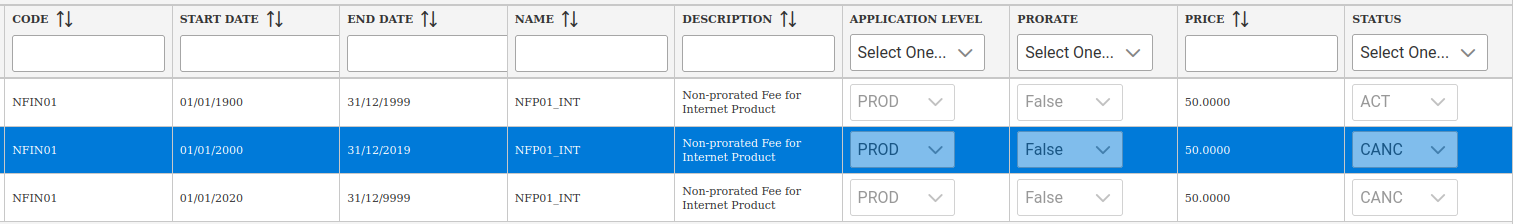
\includegraphics[width=\textwidth]{imaxes/cambio-estado-cancelado.png}
  \caption{Listado actualizado con el cambio de estado}
  \label{fig:cambio-estado-cancelado}
\end{figure}




\subsubsection{Product Type - tipo de producto}
\label{sub:product-type}

Nota: Para acceder a la pantalla que da acceso a la operativa de este tipo de entidad se desplegará la sección \emph{CATALOG} del menú principal y se seleccionará el tipo de entidad \emph{Product Type} $\rightarrow$ \emph{Product Type Definition}.

Consideramos los tipos de productos como entidades pertenecientes al catálogo de servicios propiamente dicho.

Entendemos por tipo de producto un paquete a ofertar a los clientes que tiene asociado un conjunto de tipos de cuotas y tipos de descuentos sobre esos tipos cuotas y que contiene los distintos servicios ofertados con sus correspondientes tipos de elementos facturables y tipos de promoción.

La definición completa de un tipo de producto viene dado por sí mismo y las relaciones que establece con el resto de entidades del catálogo de servicios ofertados: tipos de cuotas que aplican sobre el producto, tipos de promociones que pueden aplicar descuentos sobre esos tipos de cuotas y tipos de servicio que dependen del tipo de producto. En este apartado nos centraremos en la definición del tipo de producto \textit{per se} dejando la definición del tipo de producto con el resto de tipos de entidades para más adelante, una vez visto el resto de elementos que conforman el catálogo de servicios.

Un tipo de producto viene definido por los elementos indicados en la \tablename~\ref{tab:tipo-producto}:



\begin{table}[H]
  \centering
  \rowcolors{2}{white}{udcgray!25}
  \setlength{\leftmargini}{0.4cm}
  \resizebox{14cm}{!} {
  \begin{tabular}{|m{3cm} m{11cm}|}
  \rowcolor{udcpink!25}
  \hline
  	\textbf{Elemento} & \textbf{Descripción} \\\hline
	\textbf{CODE} & Código identificativo del tipo de producto. Es único.   \\
	\textbf{NAME} & Nombre del tipo de producto. \\
	\textbf{DESCRIPTION} & Descripción del tipo de producto. \\		
	\textbf{STATUS} & Estado del tipo del producto.
	\\\hline
  \end{tabular}
  } % end /resizebox
  \caption{Datos que definen un tipo de producto.}
  \label{tab:tipo-producto}
\end{table}

Las operaciones definidas para esta entidad son las siguientes (nota: sólo están habilitadas para usuarios con permisos de edición):
\begin{description}
\item[\underline{\textsl{\textbf{Crear nuevo tipo de producto}}}] Para crear un nuevo tipo de producto se pulsará el botón \textit{New Data} situado en la parte superior de la tabla. Aparecerá una ventana emergente que mostrará un formulario con los campos a cubrir.

\item[\underline{\textsl{\textbf{Editar tipo de producto existente}}}] Para editar un tipo de producto existente se seleccionará del listado y se pulsará el botón editar de la columna \textit{EDIT ROW} correspondiente. Se editarán los campos pertinentes directamente en la tabla para realizar las modificaciones oportunas. 

\item[\underline{\textsl{\textbf{Borrar tipo de consumo}}}] Para borrar un tipo de producto se seleccionará del listado y se pulsará el botón amarillo de borrar de la columna \textit{DEL ROW} correspondiente.
\end{description}

Todos los valores mostrados para la entidad son obligatorios y deberán cubrirse al realizar un alta o modificación. Asimismo el valor del campo CODE es único. No pueden existir dos entidades del mismo tipo con el mismo código.




\subsubsection{Service Type - tipo de servicio}
\label{sub:service-type}

Nota: Para acceder a la pantalla que da acceso a la operativa de este tipo de entidad se desplegará la sección \emph{CATALOG} del menú principal y se seleccionará el tipo de entidad \emph{Service Type} $\rightarrow$  \emph{Service Type Definition}.

Consideramos los tipos de servicios como entidades pertenecientes al catálogo de servicios propiamente dicho.

Entendemos por tipo de servicio el bien inmaterial que se le presta al cliente y que es el verdadero objetivo de la contratación.

La definición completa de un tipo de servicio viene dado por sí mismo y las relaciones que establece con el resto de entidades del catálogo de servicios ofertados: tipos de productos en los que está englobado, tipos de cuotas que pueden aplicar sobre él y los tipos de promociones que pueden aplicar descuentos sobre los distintos tipos de elementos facturables asociados al tipo de servicio. En este apartado nos centraremos en la definición del tipo de servicio \textit{per se} dejando la definición del tipo de servicio con el resto de tipos de entidades para más adelante, una vez visto el resto de elementos que conforman el catálogo de servicios.

Un tipo de servicio viene definido por los elementos indicados en la \tablename~\ref{tab:tipo-servicio}:



\begin{table}[H]
  \centering
  \rowcolors{2}{white}{udcgray!25}
  \setlength{\leftmargini}{0.4cm}
  \resizebox{14cm}{!} {
  \begin{tabular}{|m{3cm} m{11cm}|}
  \rowcolor{udcpink!25}
  \hline
  	\textbf{Elemento} & \textbf{Descripción} \\\hline
	\textbf{CODE} & Código identificativo del tipo de servicio. Es único.   \\
	\textbf{NAME} & Nombre del tipo de servicio. \\
	\textbf{DESCRIPTION} & Descripción del tipo de servicio. \\		
	\textbf{STATUS} & Estado del tipo del servicio.
	\\\hline
  \end{tabular}
  } % end /resizebox
  \caption{Datos que define un tipo de servicio.}
  \label{tab:tipo-servicio}
\end{table}

Las operaciones definidas para esta entidad son las siguientes (nota: sólo están habilitadas para usuarios con permisos de edición):
\begin{description}
\item[\underline{\textsl{\textbf{Crear nuevo tipo de producto}}}] Para crear un nuevo tipo de producto se pulsará el botón \textit{New Data} situado en la parte superior de la tabla. Aparecerá una ventana emergente que mostrará un formulario con los campos a cubrir.

\item[\underline{\textsl{\textbf{Editar tipo de producto existente}}}] Para editar un tipo de producto existente se seleccionará del listado y se pulsará el botón editar de la columna \textit{EDIT ROW} correspondiente. Se editarán los campos pertinentes directamente en la tabla para realizar las modificaciones oportunas. 

\item[\underline{\textsl{\textbf{Borrar tipo de consumo}}}] Para borrar un tipo de producto se seleccionará del listado y se pulsará el botón amarillo de borrar de la columna \textit{DEL ROW} correspondiente.
\end{description}

Todos los valores mostrados para la entidad son obligatorios y deberán cubrirse al realizar un alta o modificación. Asimismo el valor del campo CODE es único. No pueden existir dos entidades del mismo tipo con el mismo código.



\subsubsection{Promotion Type - tipo de Promoción}
\label{sub:promotion-type}

Nota: Para acceder a la pantalla que da acceso a la operativa de este tipo de entidad se desplegará la sección \emph{CATALOG} del menú principal y se seleccionará el tipo de entidad \emph{Promotion Type} $\rightarrow$  \emph{Promotion Type Definition}.

Consideramos los tipos de promociones como entidades pertenecientes al catálogo de servicios propiamente dicho.

Entendemos por tipo de promoción aquellos descuentos que pueden aplicarse sobre tipos de elementos facturables.

La definición completa de un tipo de promoción viene dado por sí mismo y las relaciones que establece con el resto de entidades del catálogo de servicios ofertados: los distintos tipos de elementos facturables sobre los que puede aplicar un descuento y las entidades facturables sobre las que aplican dichos elementos facturables.  En este apartado nos centraremos en la definición del tipo de promoción \textit{per se} dejando la definición del tipo de promoción con el resto de tipos de entidades para más adelante.

Al igual que ocurre con los tipos de cuota, los tipos de promoción pueden variar con el tiempo, modificándose las condiciones de descuento. Por lo tanto se ha considerado la necesidad de llevar un registro de estos cambios a lo largo de la vida útil de este tipo de elementos. Así pues una entidad de este tipo estará conformada por uno o varios registros con una fecha inicio y una fecha fin que definen el período en el que aplican las condiciones definidas para esa entidad. Estos registros deben ser consecutivos de forma que si existen varios registros la fecha de inicio de un registro debe ser la fecha de fin del registro anterior mas un día (salvo para el primer registro que conforma el período del ciclo de vida del elemento). De igual forma la fecha de finalización de un registro debe ser la fecha de inicio del registro siguiente menos un día (salvo para el último registro que conforma el período del ciclo de vida del elemento).


Un tipo de promoción viene definido por los elementos indicados en la \tablename~\ref{tab:tipo-promoción}.
Las operaciones definidas para esta entidad son las siguientes:

\begin{table}
  \centering
  \rowcolors{2}{white}{udcgray!25}
  \setlength{\leftmargini}{0.4cm}
  \resizebox{14cm}{!} {
  \begin{tabular}{|m{4cm} m{11cm}|}
  \rowcolor{udcpink!25}
  \hline
  	\textbf{Elemento} & \textbf{Descripción} \\\hline
  	\textbf{START DATE} & Fecha de inicio del período temporal para el que aplican las condiciones especificadas para dicho período.\\
  	\textbf{END DATE} & Fecha de finalización del período temporal para el que aplican las condiciones especificadas para dicho período.\\
  	\textbf{CODE} & Código identificativo del tipo de promoción. Es único.\\
	\textbf{NAME} & Nombre del tipo de promoción.\\
	\textbf{DESCRIPTION} & Descripción del tipo de promoción.\\
	\textbf{APPLICATION LEVEL} & Nivel de aplicación del tipo de promoción, esto es, a qué entidad facturable va asociado. Los niveles de aplicación están definidos en la correspondiente entidad de \emph{PARAMETERS} definida en la sección \ref{sub:parametrizacion}.\\	
	\textbf{DISCOUNT TYPE} & Indica el tipo de descuento a aplicar por el tipo de promoción. Los distintos tipos de descuento definidos en la correspondiente entidad de \emph{PARAMETERS} definida en la sección \ref{sub:parametrizacion}..\\
	\textbf{DISCOUNT VALUE} & Descuento a aplicar en función del tipo de descuento definido en el tipo de promoción (volumen, unidades, porcentaje\dots.\\
	\textbf{STATUS} & Estado del tipo de promoción.	
	\\\hline
  \end{tabular}
  } % end /resizebox
  \caption{Datos que define un tipo de promoción.}
  \label{tab:tipo-promoción}
\end{table}

\begin{description}
\item[\underline{\textsl{\textbf{Buscar un tipo de promoción existente}}}] Esta operación está disponible para todos los usuarios de la aplicación.
Puesto que los tipos de promoción son entidades con histórico, por motivos de operatividad no se muestra el listado de todas las entidades del sistema por defecto, si no que se establecen unos criterios de búsqueda para seleccionar el tipo de promoción a consultar. Para ello se define un área de búsqueda en los que se definen los criterios de búsqueda a tener en cuenta:
\begin{itemize}
\item Buscar todos los históricos de los tipos de consumo. Se realizará una búsqueda de todos los históricos de los distintos tipos de consumo.
\item Buscar por fecha. Se realizará una búsqueda de los históricos de todos los tipos de consumo existentes en el sistema para los que la fecha de búsqueda definida se encuentre entre la fecha de inicio y fin del registro de histórico. Opción marcada por defecto
\end{itemize}

Pulsando el botón \emph{Search} se mostrará un panel emergente con el listado de los registros encontrados. Seleccionaremos el elemento sobre el que queramos operar pulsando el botón amarillo de la columna \emph{Show Historic} y se mostrará el área de históricos de la entidad con los distintos registros de histórico existentes de forma análogo a lo ya visto en la sección \ref{sub:fee-type}

\item[\underline{\textsl{\textbf{Crear nuevo tipo de promoción}}}] Esta operación sólo está disponible para usuarios con permisos de edición.
Para crear un nuevo consumo se pulsará el botón \textit{New Data} situado en la parte superior de la tabla. Aparecerá una ventana emergente que mostrará un formulario con los campos a cubrir. Por defecto se establecen como fecha de inicio y fin del nuevo tipo de cuota las fechas 01/01/1900 y 31/12/9999.

\item[\underline{\textsl{\textbf{Editar registro de histórico de un tipo de promoción existente}}}] Esta operación sólo está disponible para usuarios con permisos de edición.
Para editar un tipo de consumo existente se seleccionará del listado y se pulsará el botón editar de la columna \textit{EDIT ROW} correspondiente. Se editarán los campos pertinentes directamente en la tabla para realizar las modificaciones oportunas teniendo en cuenta los criterios de fechas establecidos (definidos en la sección \ref{sub:histórico-conceptos} de la página \pageref{sub:histórico-conceptos}).

\item[\underline{\textsl{\textbf{Añadir registro de histórico de un tipo de promoción existente}}}] Esta operación sólo está disponible para usuarios con permisos de edición.
Para añadir un nuevo registro de histórico sobre tipo de consumo existente se seleccionará del listado el registro en el que se ubicará el nuevo registro a añadir 
y se pulsará el botón añadir de la columna \textit{ADD ROW} correspondiente. Aparecerá una nueva ventana emergente como la que se muestra en la operación de creación, pero con los campos cubiertos con la información del registro sobre el que se va a añadir el nuevo registro y se realizarán las modificaciones oportunas teniendo en cuenta los criterios de fechas establecidos (definidos en la sección \ref{sub:histórico-conceptos} de la página \pageref{sub:histórico-conceptos}).

\item[\underline{\textsl{\textbf{Borrar registro de histórico del tipo de promoción}}}] Esta operación sólo está disponible para usuarios con permisos de edición.
Para borrar un registro de histórico del tipo de consumo se seleccionará del listado el registro a borrar y se pulsará el botón amarillo de borrar de la columna \textit{DEL ROW} correspondiente.

\item[\underline{\textsl{\textbf{Borrar el tipo de promoción}}}] Esta operación sólo está disponible para usuarios con permisos de edición.
Para borrar completamente un tipo de cuota se deben borrar uno a uno todos los registros de histórico del tipo de cuota según lo indicado en el punto anterior.
\end{description}

Todos los valores mostrados para la entidad son obligatorios y deberán cubrirse al realizar un alta o modificación. Asimismo el valor del campo CODE es único. No pueden existir dos entidades del mismo tipo con el mismo código.

La realización de las distintas operaciones es análogo a lo visto para las operaciones de los tipos de cuotas. Para más información consulte la sección \ref{sub:fee-type}.


\subsubsection{Product Fee Type - Relación entre tipo de Producto y de Cuota}
\label{sub:product-fee-type-relation}

Nota: Para acceder a la pantalla que da acceso a la operativa de este tipo de entidad se desplegará la sección \emph{CATALOG} del menú principal y se seleccionará el tipo de entidad \emph{Product Type} $\rightarrow$  \emph{Product Fee Type}.


A continuación veremos cómo gestionar las distintas relaciones que se establecen entre un tipo de producto y los tipos de cuotas que pueden asociarse al tipo de producto dado.


En la parte superior de la pantalla se encuentra el área de búsqueda. Pulsando el botón verde \emph{SEARCH} aparece un listado de todos los productos del sistema. Seleccionaremos el tipo de producto sobre el que queramos consultar las relaciones de las entidades pulsando el botón amarillo de la columna \emph{Show Data}. A continuación se visualizará el área de relaciones del producto en los que se muestran los tipos de cuotas para los que existe una relación con el producto (ver \figurename~\ref{fig:area-relacion-tipos-entidades}).


\begin{figure}[H]
  \centering
  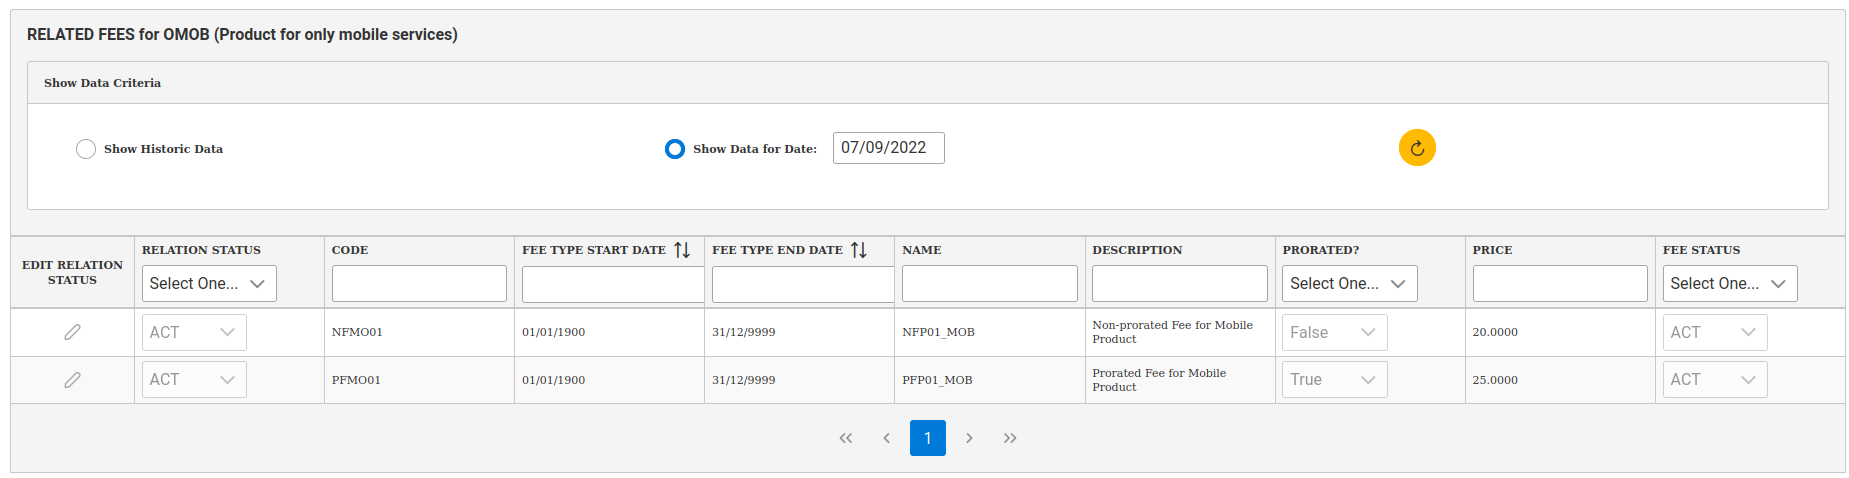
\includegraphics[width=\textwidth]{imaxes/area-relacion-tipos-entidades.png}
  \caption{Área que muestra los tipos de entidad cuota relacionada con el producto}
  \label{fig:area-relacion-tipos-entidades}
\end{figure}



Al ser el tipo de cuota una entidad con registro de histórico en el área de relaciones se muestran por defecto los registros para los que la fecha definida en el área de visualización de la entidad relacionada (que por defecto es la fecha actual) se encuentra comprendida en el período del histórico. Si queremos mostrar todos los registros de histórico de las distintas entidades relacionadas seleccionaremos la opción de \emph{Show Historic Data} y pulsaremos el botón de refrescar que se encuentra a la derecha del área de criterios de visualización. Lo mismo si queremos que se muestren los históricos para otra fecha distinta de la especificada por defecto: bastará con modificar la fecha y pulsar el botón de refrescar.

Si accedemos a la vista con un usuario con permisos de edición se mostrará otro listado con los tipos de cuota con nivel de aplicación producto para los que no se ha establecido relación con el tipo de producto consultado, así como dos botones, uno con una flecha apuntando hacia arriba y otro con una flecha apuntando hacia abajo. Estos botones permitirán añadir un tipo de cuota a la relación con el producto o eliminar dicha relación respectivamente. 



\begin{figure}[H]
  \centering
  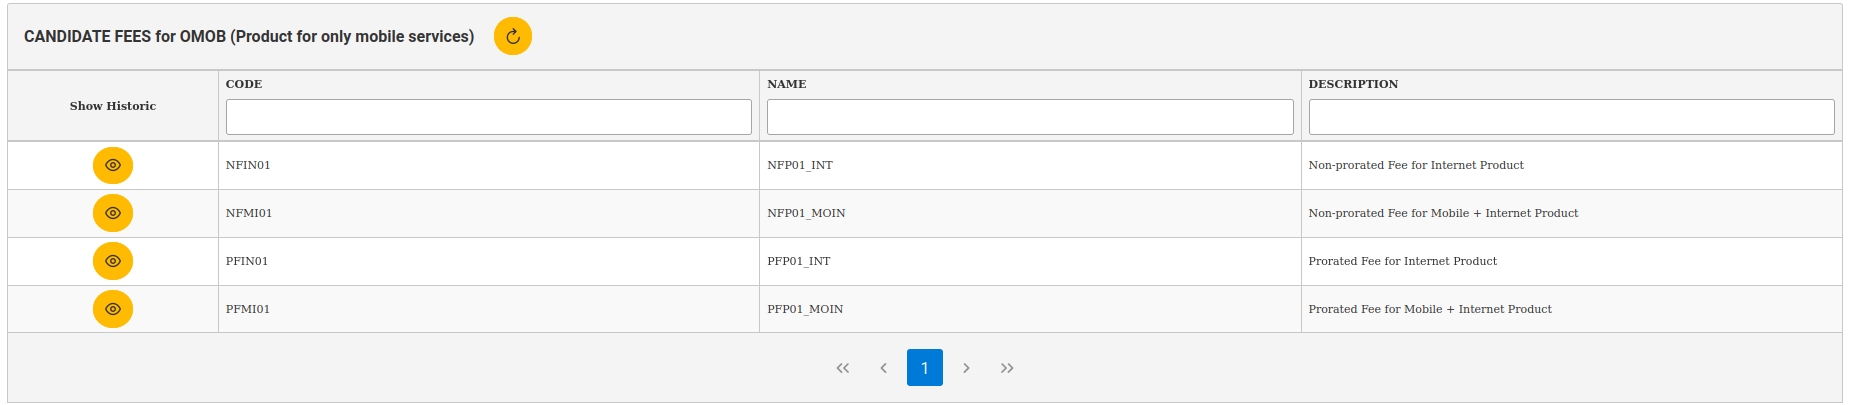
\includegraphics[width=\textwidth]{imaxes/area-tipos-entidades-candidatas.png}
  \caption{Área que muestra los tipos de entidad cuota candidatas a establecer relación con el producto}
  \label{fig:area-tipos-entidades-candidatas}
\end{figure}



\begin{figure}[H]
  \centering
  \includegraphics[width=0.15\textwidth]{imaxes/botones-añadir-eliminar-relacion-tipos.png}
  \caption{Detalle de los botones para gestionar las relaciones: a la izquierda el botón de añadir relación, a la derecha el botón de eliminar relación}
  \label{fig:botones-añadir-eliminar-relacion-tipos}
\end{figure}

A mayores el listado de entidades relacionadas permite editar el estado de la relación mientras que en el listado de candidatos existe un botón que permite ver el histórico de la entidad candidata, siempre que el usuario tenga permisos de edición.



Las operaciones definidas para esta vista son las siguientes (nota: sólo están habilitadas para usuarios con permisos de edición):
\begin{description}
\item[\underline{\textsl{\textbf{Añadir una nueva entidad tipo cuota a la relación}}}] Para añadir una nueva relación seleccionaremos el tipo de cuota deseado del listado de candidatos y pulsaremos el botón de la flecha que apunta hacia arriba (hacia el listado de entidades relacionadas). Se eliminará el registro del listado de candidatos y se añadirá al listado de tipos de cuotas relacionadas.

\item[\underline{\textsl{\textbf{Eliminar una entidad tipo cuota existente de la relación}}}] Para eliminar una relación existente seleccionaremos el tipo de cuota deseado del listado de relaciones y pulsaremos el botón de la flecha que apunta hacia abajo (hacia el listado de entidades candidatas). Se eliminará el registro del listado de relaciones y se añadirá al listado de tipos de cuotas candidatas.

\item[\underline{\textsl{\textbf{Editar el estado de la relación de histórico de un tipo de cuota existente}}}] Para editar el estado de la relación se seleccionará la entidad del tipo cuota deseada del listado de entidades relacionadas y se pulsará el botón editar de la columna \textit{EDIT RELATION STATUS} correspondiente. Se editará el campo \emph{RELATION STATUS}  pertinentes directamente en la tabla para realizar las modificaciones oportunas.

\item[\underline{\textsl{\textbf{Visualizar el registro de históricos de un tipo de cuota candidata}}}] Para visualizar todos los históricos de un tipo de cuota candidata se seleccionará la entidad del tipo cuota deseada del listado de entidades relacionadas y se pulsará el botón amarillo de la columna \textit{SHOW HISTORICS}. Se mostrará un panel que muestra el listado de históricos para la entidad seleccionada.
\end{description}


\subsubsection{Product Service Type - Relación entre tipo de Producto y de Servicio}
\label{sub:product-service-type-relation}

Nota: Para acceder a la pantalla que da acceso a la operativa de este tipo de entidad se desplegará la sección \emph{CATALOG} del menú principal y se seleccionará el tipo de entidad \emph{Product Type} $\rightarrow$  \emph{Promotion Service Type}.


A continuación veremos cómo gestionar las distintas relaciones que se establecen entre un tipo de producto y los tipos de servicio que pueden contener.


En la parte superior de la pantalla se encuentra el área de búsqueda. Pulsando el botón verde \emph{SEARCH} aparece un listado de todos los productos del sistema. Seleccionaremos el tipo de producto sobre el que queramos consultar las relaciones de las entidades pulsando el botón amarillo de la columna \emph{Show Data}. A continuación se visualizará el área de relaciones del producto en los que se muestran los tipos de servicio para los que existe una relación con el producto.

Si accedemos a la vista con un usuario con permisos de edición se mostrará otro listado con los tipos de servicio para los que no se ha establecido relación con el tipo de producto consultado, así como dos botones, uno con una flecha apuntando hacia arriba y otro con una flecha apuntando hacia abajo. Estos botones permitirán añadir un tipo de servicio a la relación con el producto o eliminar dicha relación respectivamente. 

A mayores el listado de entidades relacionadas permite editar el estado de la relación mientras que en el listado de candidatos existe un botón que permite ver el histórico de la entidad candidata, siempre que el usuario tenga permisos de edición.


Las operaciones definidas para esta vista son las siguientes (nota: sólo están habilitadas para usuarios con permisos de edición):
\begin{description}
\item[\underline{\textsl{\textbf{Añadir una nueva entidad tipo servicio a la relación}}}] Para añadir una nueva relación seleccionaremos el tipo de servicio deseado del listado de candidatos y pulsaremos el botón de la flecha que apunta hacia arriba (hacia el listado de entidades relacionadas). Se eliminará el registro del listado de candidatos y se añadirá al listado de tipos de servicio relacionados.

\item[\underline{\textsl{\textbf{Eliminar una entidad tipo servicio existente de la relación}}}] Para eliminar una relación existente seleccionaremos el tipo de servicio deseado del listado de relaciones y pulsaremos el botón de la flecha que apunta hacia abajo (hacia el listado de entidades candidatas). Se eliminará el registro del listado de relaciones y se añadirá al listado de tipos de servicios candidatas.

\item[\underline{\textsl{\textbf{Editar el estado de la relación de histórico de un tipo de servicio existente}}}] Para editar el estado de la relación se seleccionará la entidad del tipo servicio de consumo deseado del listado de entidades relacionadas y se pulsará el botón editar de la columna \textit{EDIT RELATION STATUS} correspondiente. Se editará el campo \emph{RELATION STATUS} pertinentes directamente en la tabla para realizar las modificaciones oportunas.
\end{description}



\subsubsection{Product Promotion Type - Relación entre tipo de Producto y de Promoción}
\label{sub:product-promotion-type-relation}

Nota: Para acceder a la pantalla que da acceso a la operativa de este tipo de entidad se desplegará la sección \emph{CATALOG} del menú principal y se seleccionará el tipo de entidad \emph{Product Type} $\rightarrow$  \emph{Product Promotion Type}.


A continuación veremos cómo gestionar las distintas relaciones que se establecen entre un tipo de producto y los tipos de promociones que pueden asociarse al tipo de producto dado.


En la parte superior de la pantalla se encuentra el área de búsqueda. Pulsando el botón verde \emph{SEARCH} aparece un listado de todos los productos del sistema. Seleccionaremos el tipo de producto sobre el que queramos consultar las relaciones de las entidades pulsando el botón amarillo de la columna \emph{Show Data}. A continuación se visualizará el área de relaciones del producto en los que se muestran los tipos de promociones para los que existe una relación con el producto.

Al ser el tipo de promoción una entidad con registro de histórico en el área de relaciones se muestran por defecto los registros para los que la fecha definida en el área de visualización de la entidad relacionada (que por defecto es la fecha actual) se encuentra comprendida en el período del histórico. Si queremos mostrar todos los registros de histórico de las distintas entidades relacionadas seleccionaremos la opción de Show Historic Data y pulsaremos el botón de refrescar que se encuentra a la derecha del área de criterios de visualización. Lo mismo si queremos que se muestren los históricos para otra fecha distinta de la especificada por defecto: bastará con modificar la fecha y pulsar el botón de refrescar.

Si accedemos a la vista con un usuario con permisos de edición se mostrará otro listado con los tipos de promoción con nivel de aplicación producto para los que no se ha establecido relación con el tipo de producto consultado, así como dos botones, uno con una flecha apuntando hacia arriba y otro con una flecha apuntando hacia abajo. Estos botones permitirán añadir un tipo de promoción a la relación con el producto o eliminar dicha relación respectivamente. 

A mayores el listado de entidades relacionadas permite editar el estado de la relación mientras que en el listado de candidatos existe un botón que permite ver el histórico de la entidad candidata, siempre que el usuario cuente con permisos de edición.


Las operaciones definidas para esta vista son las siguientes (nota: sólo están habilitadas para usuarios con permisos de edición):
\begin{description}
\item[\underline{\textsl{\textbf{Añadir una nueva entidad tipo promoción a la relación}}}] Para añadir una nueva relación seleccionaremos el tipo de promoción deseado del listado de candidatos y pulsaremos el botón de la flecha que apunta hacia arriba (hacia el listado de entidades relacionadas). Se eliminará el registro del listado de candidatos y se añadirá al listado de tipos de cuotas relacionadas.

\item[\underline{\textsl{\textbf{Eliminar una entidad tipo promoción existente de la relación}}}] Para eliminar una relación existente seleccionaremos el tipo de promoción deseado del listado de relaciones y pulsaremos el botón de la flecha que apunta hacia abajo (hacia el listado de entidades candidatas). Se eliminará el registro del listado de relaciones y se añadirá al listado de tipos de promociones candidatas.

\item[\underline{\textsl{\textbf{Editar el estado de la relación de histórico de un tipo de promoción existente}}}] Para editar el estado de la relación se seleccionará la entidad del tipo promoción  deseada del listado de entidades relacionadas y se pulsará el botón editar de la columna \textit{EDIT RELATION STATUS} correspondiente. Se editará el campo \emph{RELATION STATUS}  pertinentes directamente en la tabla para realizar las modificaciones oportunas.

\item[\underline{\textsl{\textbf{Visualizar el registro de históricos de un tipo de promoción candidata}}}] Para visualizar todos los históricos de un tipo de promoción candidata se seleccionará la entidad del tipo promoción deseada del listado de entidades relacionadas y se pulsará el botón amarillo de la columna \textit{SHOW HISTORICS}. Se mostrará un panel que muestra el listado de históricos para la entidad seleccionada. 
\end{description}


\subsubsection{Service Fee Type - Relación entre tipo de Servicio y de Cuota}
\label{sub:service-fee-type-relation}

Nota: Para acceder a la pantalla que da acceso a la operativa de este tipo de entidad se desplegará la sección \emph{CATALOG} del menú principal y se seleccionará el tipo de entidad \emph{Service Type} $\rightarrow$  \emph{Service Fee Type}.


A continuación veremos cómo gestionar las distintas relaciones que se establecen entre un tipo de servicio y los tipos de cuotas que pueden asociarse al tipo de servicio dado.


En la parte superior de la pantalla se encuentra el área de búsqueda. Pulsando el botón verde \emph{SEARCH} aparece un listado de todos los servicios del sistema. Seleccionaremos el tipo de servicio sobre el que queramos consultar las relaciones de las entidades pulsando el botón amarillo de la columna \emph{Show Data}. A continuación se visualizará el área de relaciones del producto en los que se muestran los tipos de cuotas para los que existe una relación con el servicio.

Al ser el tipo de cuota una entidad con registro de histórico en el área de relaciones se muestran por defecto los registros para los que la fecha definida en el área de visualización de la entidad relacionada (que por defecto es la fecha actual) se encuentra comprendida en el período del histórico. Si queremos mostrar todos los registros de histórico de las distintas entidades relacionadas seleccionaremos la opción de Show Historic Data y pulsaremos el botón de refrescar que se encuentra a la derecha del área de criterios de visualización. Lo mismo si queremos que se muestren los históricos para otra fecha distinta de la especificada por defecto: bastará con modificar la fecha y pulsar el botón de refrescar.

Si accedemos a la vista con un usuario con permisos de edición se mostrará otro listado con los tipos de cuota con nivel de aplicación servicio para los que no se ha establecido relación con el tipo de servicio consultado, así como dos botones, uno con una flecha apuntando hacia arriba y otro con una flecha apuntando hacia abajo. Estos botones permitirán añadir un tipo de cuota a la relación con el servicio o eliminar dicha relación respectivamente. 

A mayores el listado de entidades relacionadas permite editar el estado de la relación mientras que en el listado de candidatos existe un botón que permite ver el histórico de la entidad candidata, siempre que el usuario cuente con permisos de edición.



Las operaciones definidas para esta vista son las siguientes (nota: sólo están habilitadas para usuarios con permisos de edición):
\begin{description}
\item[\underline{\textsl{\textbf{Añadir una nueva entidad tipo cuota a la relación}}}] Para añadir una nueva relación seleccionaremos el tipo de cuota deseado del listado de candidatos y pulsaremos el botón de la flecha que apunta hacia arriba (hacia el listado de entidades relacionadas). Se eliminará el registro del listado de candidatos y se añadirá al listado de tipos de cuotas relacionadas.

\item[\underline{\textsl{\textbf{Eliminar una entidad tipo cuota existente de la relación}}}] Para eliminar una relación existente seleccionaremos el tipo de cuota deseado del listado de relaciones y pulsaremos el botón de la flecha que apunta hacia abajo (hacia el listado de entidades candidatas). Se eliminará el registro del listado de relaciones y se añadirá al listado de tipos de cuotas candidatas.

\item[\underline{\textsl{\textbf{Editar el estado de la relación de histórico de un tipo de cuota existente}}}] Para editar el estado de la relación se seleccionará la entidad del tipo cuota deseada del listado de entidades relacionadas y se pulsará el botón editar de la columna \textit{EDIT RELATION STATUS} correspondiente. Se editará el campo \emph{RELATION STATUS}  pertinentes directamente en la tabla para realizar las modificaciones oportunas.

\item[\underline{\textsl{\textbf{Visualizar el registro de históricos de un tipo de cuota candidata}}}] Para visualizar todos los históricos de un tipo de cuota candidata se seleccionará la entidad del tipo cuota deseada del listado de entidades relacionadas y se pulsará el botón amarillo de la columna \textit{SHOW HISTORICS}. Se mostrará un panel que muestra el listado de históricos para la entidad seleccionada.
\end{description}



\subsubsection{Service Promotion Type - Relación entre tipo de Servicio y de Promoción}
\label{sub:service-promotion-type-relation}

Nota: Para acceder a la pantalla que da acceso a la operativa de este tipo de entidad se desplegará la sección \emph{CATALOG} del menú principal y se seleccionará el tipo de entidad \emph{Service Type} $\rightarrow$  \emph{Service Promotion Type}.


A continuación veremos cómo gestionar las distintas relaciones que se establecen entre un tipo de servicio y los tipos de promociones que pueden asociarse al tipo de servicio dado.


En la parte superior de la pantalla se encuentra el área de búsqueda. Pulsando el botón verde \emph{SEARCH} aparece un listado de todos los servicios del sistema. Seleccionaremos el tipo de producto sobre el que queramos consultar las relaciones de las entidades pulsando el botón amarillo de la columna \emph{Show Data}. A continuación se visualizará el área de relaciones del servicio en los que se muestran los tipos de promoción para los que existe una relación con el servicio.

Al ser el tipo de promoción una entidad con registro de histórico en el área de relaciones se muestran por defecto los registros para los que la fecha definida en el área de visualización de la entidad relacionada (que por defecto es la fecha actual) se encuentra comprendida en el período del histórico. Si queremos mostrar todos los registros de histórico de las distintas entidades relacionadas seleccionaremos la opción de Show Historic Data y pulsaremos el botón de refrescar que se encuentra a la derecha del área de criterios de visualización. Lo mismo si queremos que se muestren los históricos para otra fecha distinta de la especificada por defecto: bastará con modificar la fecha y pulsar el botón de refrescar.

Si accedemos a la vista con un usuario con permisos de edición se mostrará otro listado con los tipos de promoción con nivel de aplicación servicio para los que no se ha establecido relación con el tipo de servicio consultado, así como dos botones, uno con una flecha apuntando hacia arriba y otro con una flecha apuntando hacia abajo. Estos botones permitirán añadir un tipo de promoción a la relación con el servicio o eliminar dicha relación respectivamente. 

A mayores el listado de entidades relacionadas permite editar el estado de la relación mientras que en el listado de candidatos existe un botón que permite ver el histórico de la entidad candidata, siempre que el usuario cuente con permisos de edición


Las operaciones definidas para esta vista son las siguientes (nota: sólo están habilitadas para usuarios con permisos de edición):
\begin{description}
\item[\underline{\textsl{\textbf{Añadir una nueva entidad tipo promoción a la relación}}}] Para añadir una nueva relación seleccionaremos el tipo de promoción deseado del listado de candidatos y pulsaremos el botón de la flecha que apunta hacia arriba (hacia el listado de entidades relacionadas). Se eliminará el registro del listado de candidatos y se añadirá al listado de tipos de cuotas relacionadas.

\item[\underline{\textsl{\textbf{Eliminar una entidad tipo promoción existente de la relación}}}] Para eliminar una relación existente seleccionaremos el tipo de promoción deseado del listado de relaciones y pulsaremos el botón de la flecha que apunta hacia abajo (hacia el listado de entidades candidatas). Se eliminará el registro del listado de relaciones y se añadirá al listado de tipos de promociones candidatas.

\item[\underline{\textsl{\textbf{Editar el estado de la relación de histórico de un tipo de promoción existente}}}] Para editar el estado de la relación se seleccionará la entidad del tipo promoción  deseada del listado de entidades relacionadas y se pulsará el botón editar de la columna \textit{EDIT RELATION STATUS} correspondiente. Se editará el campo \emph{RELATION STATUS}  pertinentes directamente en la tabla para realizar las modificaciones oportunas.

\item[\underline{\textsl{\textbf{Visualizar el registro de históricos de un tipo de promoción candidata}}}]
Para visualizar todos los históricos de un tipo de promoción candidata se seleccionará la entidad del tipo promoción deseada del listado de entidades relacionadas y se pulsará el botón amarillo de la columna \textit{SHOW HISTORICS}. Se mostrará un panel que muestra el listado de históricos para la entidad seleccionada. 
\end{description}


\subsubsection{Promotion Fee Type - Relación entre tipo de Promoción y de Cuota}
\label{sub:promotion-fee-type-relation}

Nota: Para acceder a la pantalla que da acceso a la operativa de este tipo de entidad se desplegará la sección \emph{CATALOG} del menú principal y se seleccionará el tipo de entidad \emph{Promotion Type} $\rightarrow$  \emph{Promotion Fee Type Discount}.


A continuación veremos cómo gestionar las distintas relaciones que se establecen entre un tipo de promoción y los tipos de consumos que pueden asociarse al tipo de promoción dado.


En la parte superior de la pantalla se encuentra el área de búsqueda. Puesto que los tipos de promoción son entidades con histórico, dicha área contendrá los criterios de búsqueda según lo especificado en las secciones relativas a los tipos de entidad con histórico \ref{sub:fee-type} y \ref{sub:promotion-type}. 
Seleccionaremos el tipo de promoción sobre el que queramos consultar las relaciones de las entidades pulsando el botón amarillo de la columna \emph{Show Data}. A continuación se visualizará el área de relaciones de la promoción en los que se muestran los tipos de cuotas para los que existe una relación con la promoción.


Al ser el tipo de cuota una entidad con registro de histórico en el área de relaciones se muestran por defecto los registros para los que la fecha definida en el área de visualización de la entidad relacionada (que por defecto es la fecha actual) se encuentra comprendida en el período del histórico. Si queremos mostrar todos los registros de histórico de las distintas entidades relacionadas seleccionaremos la opción de Show Historic Data y pulsaremos el botón de refrescar que se encuentra a la derecha del área de criterios de visualización. Lo mismo si queremos que se muestren los históricos para otra fecha distinta de la especificada por defecto: bastará con modificar la fecha y pulsar el botón de refrescar.

Si accedemos a la vista con un usuario con permisos de edición se mostrará otro listado con los tipos de cuota con el mismo nivel de aplicación que la promoción para los que no se ha establecido relación con el tipo de promoción consultado, así como dos botones, uno con una flecha apuntando hacia arriba y otro con una flecha apuntando hacia abajo. Estos botones permitirán añadir un tipo de cuota a la relación con el promoción o eliminar dicha relación respectivamente. 

A mayores el listado de entidades relacionadas permite editar el estado de la relación mientras que en el listado de candidatos existe un botón que permite ver el histórico de la entidad candidata, siempre que el usuario disponga de permisos de edición.


Las operaciones definidas para esta vista son las siguientes (nota: sólo están habilitadas para usuarios con permisos de edición):
\begin{description}
\item[\underline{\textsl{\textbf{Añadir una nueva entidad tipo cuota a la relación}}}] Para añadir una nueva relación seleccionaremos el tipo de cuota deseado del listado de candidatos y pulsaremos el botón de la flecha que apunta hacia arriba (hacia el listado de entidades relacionadas). Se eliminará el registro del listado de candidatos y se añadirá al listado de tipos de cuotas relacionadas.

\item[\underline{\textsl{\textbf{Eliminar una entidad tipo cuota existente de la relación}}}] Para eliminar una relación existente seleccionaremos el tipo de cuota deseado del listado de relaciones y pulsaremos el botón de la flecha que apunta hacia abajo (hacia el listado de entidades candidatas). Se eliminará el registro del listado de relaciones y se añadirá al listado de tipos de promociones candidatas.

\item[\underline{\textsl{\textbf{Editar el estado de la relación de histórico de un tipo de cuota existente}}}] Para editar el estado de la relación se seleccionará la entidad del tipo cuota  deseada del listado de entidades relacionadas y se pulsará el botón editar de la columna \textit{EDIT RELATION STATUS} correspondiente. Se editará el campo \emph{RELATION STATUS} pertinente directamente en la tabla para realizar las modificaciones oportunas.

\item[\underline{\textsl{\textbf{Visualizar el registro de históricos de un tipo de cuota candidata}}}] Para visualizar todos los históricos de un tipo de cuota candidata se seleccionará la entidad del tipo cuota deseada del listado de entidades relacionadas y se pulsará el botón amarillo de la columna \textit{SHOW HISTORICS}. Se mostrará un panel que muestra el listado de históricos para la entidad seleccionada. 
\end{description}



\subsubsection{Promotion Consumption Type - Relación entre tipo de Promoción y de Consumo}
\label{sub:promotion-consumption-type-relation}

Nota: Para acceder a la pantalla que da acceso a la operativa de este tipo de entidad se desplegará la sección \emph{CATALOG} del menú principal y se seleccionará el tipo de entidad \emph{Promotion Type} $\rightarrow$  \emph{Promotion Consumption Type Discount}.


A continuación veremos cómo gestionar las distintas relaciones que se establecen entre un tipo de promoción y los tipos de consumos que pueden asociarse al tipo de promoción dado.


En la parte superior de la pantalla se encuentra el área de búsqueda. Puesto que los tipos de promoción son entidades con histórico, dicha área contendrá los criterios de búsqueda según lo especificado en las secciones relativas a los tipos de entidad con histórico \ref{sub:fee-type} y \ref{sub:promotion-type}. 
Seleccionaremos el tipo de promoción sobre el que queramos consultar las relaciones de las entidades pulsando el botón amarillo de la columna \emph{Show Data}. A continuación se visualizará el área de relaciones de la promoción en los que se muestran los tipos de consumos para los que existe una relación con la promoción.


Si accedemos a la vista con un usuario con permisos de edición se mostrará otro listado con los tipos de consumo con el mismo nivel de aplicación que la promoción para los que no se ha establecido relación con el tipo de promoción consultado, así como dos botones, uno con una flecha apuntando hacia arriba y otro con una flecha apuntando hacia abajo. Estos botones permitirán añadir un tipo de consumo a la relación con el promoción o eliminar dicha relación respectivamente. 

A mayores el listado de entidades relacionadas permite editar el estado de la relación, siempre que el usuario disponga de permisos de edición.


Las operaciones definidas para esta vista son las siguientes (nota: sólo están habilitadas para usuarios con permisos de edición):
\begin{description}
\item[\underline{\textsl{\textbf{Añadir una nueva entidad tipo consumo a la relación}}}] Para añadir una nueva relación seleccionaremos el tipo de consumo deseado del listado de candidatos y pulsaremos el botón de la flecha que apunta hacia arriba (hacia el listado de entidades relacionadas). Se eliminará el registro del listado de candidatos y se añadirá al listado de tipos de consumos relacionadas.

\item[\underline{\textsl{\textbf{Eliminar una entidad tipo consumo existente de la relación}}}] Para eliminar una relación existente seleccionaremos el tipo de consumo deseado del listado de relaciones y pulsaremos el botón de la flecha que apunta hacia abajo (hacia el listado de entidades candidatas). Se eliminará el registro del listado de relaciones y se añadirá al listado de tipos de promociones candidatas.

\item[\underline{\textsl{\textbf{Editar el estado de la relación de histórico de un tipo de consumo existente}}}] Para editar el estado de la relación se seleccionará la entidad del tipo consumo  deseada del listado de entidades relacionadas y se pulsará el botón editar de la columna \textit{EDIT RELATION STATUS} correspondiente. Se editará el campo \emph{RELATION STATUS} pertinente directamente en la tabla para realizar las modificaciones oportunas.
\end{description}



\subsection{Contratación}
\label{sub:contratacion}

Las contrataciones del sistema están formadas por la aplicación de las definiciones vistas en el catálogo al mundo real para satisfacer las necesidades de un cliente de la empresa.

Para ello se cuenta con la cartera de clientes, entidad conformada por los distintos clientes de la empresa que han contratado diferentes productos y a los que la empresa presta los servicios contratados.

Un cliente puede tener una o varias cuentas, que son las que definen el conjunto de contrataciones de los distintos productos, servicios, cuotas y promociones específicas para dicho cliente.

Puesto que los elementos de contratación pueden variar (y mucho) a lo largo de su ciclo de vida, se han definido todos ellos como elementos con histórico, por lo que aplican las restricciones relativas a los registros de histórico indicadas en secciones anteriores.

Se definen cinco estados distintos para las entidades de contratación:
\begin{description}
\item[ACTIVE] Estado activo. Para las entidades de contratación que están en vigencia.
\item[CANCEL] Estado cancelado. Para las entidades de contratación que han cursado baja.
\item[PEND] Estado pendiente. Para las entidades de contratación pendientes de finalizar su proceso de provisión. Este estado se ha definido con vistas a una interacción con un sistema de provisión a desarrollar en el futuro.
\item[SUSP] Estado suspendido. Para las entidades de contratación que actualmente tienen su estado suspendido, por ejemplo una suspensión temporal solicitada por el cliente porque durante un período de tiempo no va a usar un determinado servicio.
\item[DEB] Estado deuda. Para las entidades de contratación cuyo cliente ha recurrido en impagos.
\end{description}


Todos los usuarios del sistema tienen acceso a los elementos de contratación, pero aquellos que tengan permisos de edición (perfil ADMIN o MODIF) podrán gestionarlos (realizar altas, bajas y modificaciones). Los usuarios con el perfil READ sólo podrán acceder en modo consulta, y no se mostrarán habilitados los correspondientes botones para las operaciones de gestión. Por comodidad las imágenes que proceden a ilustrar esta sección se corresponderán con el acceso a las vistas de un usuario con permisos de edición. Los usuarios sin estos permisos verán la misma pantalla pero sin los botones que permiten la gestión de los datos.

A continuación veremos en detalle cada una de las vistas que conforman los distintos elementos de la contratación a los que se accede a través del menú  \emph{CONTRACT}. Todas las vistas están orientadas a consultar una instancia en particular, ya que el volumen de elementos contratados deberá exceder con creces el volumen de productos contratados y mostrar todos los elementos en una única vista haría inmanejable el sistema.



\subsubsection{Customer - Clientes}
\label{sub:customer}

Esta vista muestra la información relativa a los clientes contenidos en la cartera de clientes de la empresa. La \tablename~\ref{tab:cliente} recoge los elementos más relevantes en la definición de un cliente.
Las operaciones definidas para esta entidad son las siguientes:

\begin{table}
  \centering
  \rowcolors{2}{white}{udcgray!25}
  \setlength{\leftmargini}{0.4cm}
  \resizebox{14cm}{!} {
  \begin{tabular}{|m{6cm} m{8cm}|}
  \rowcolor{udcpink!25}
  \hline
  	\textbf{Elemento} & \textbf{Descripción} \\\hline
  	\textbf{START DATE} & Fecha de inicio del período temporal para el que aplican las condiciones especificadas para dicho período.\\
  	\textbf{END DATE} & Fecha de finalización del período temporal para el que aplican las condiciones especificadas para dicho período.\\
	\textbf{CLIENT TYPE} & Tipo de cliente asociado al cliente.\\
	\textbf{CLIENT ID} & Identificador unívoco del cliente generado por la aplicación.\\
	\textbf{NAME} & Nombre del cliente.\\
	\textbf{1st SURNAME} & Primer apellido del cliente.\\
	\textbf{2nd SURNAME} & Segundo apellido del cliente.\\
	\textbf{IDENTITY CARD} & Número del documento de identificación.\\	
	\textbf{ADDRESS}, \textbf{CITY}, \textbf{STATE}, \textbf{POST CODE}, \textbf{COUNTRY}  & Datos relativos a la dirección del cliente.\\	
	\textbf{CONTACT PHONE} & Número de teléfono de contacto (no obligatorio).\\
	\textbf{EMAIL} & Dirección de correo electrónico (no obligatorio).\\
	\textbf{IBAN}, \textbf{BANK ENTITY}, \textbf{BANK BRANCH}, \textbf{BANK CONTROL DIGIT}, \textbf{BANK ACCOUNT NUMBER} & Cuenta corriente del cliente (no obligatorio).\\
	\textbf{ACTIVE DATE} & Fecha de activación del cliente. Común a todos los registros de histórico. Sólo cubierta cuando el cliente se ha activado en el sistema.\\
	\textbf{CANCELLED DATE} & Fecha de baja del cliente. Común a todos los registros de histórico. Sólo cubierta cuando el cliente ha cursado baja (estado cancelado).\\	
	\textbf{STATUS} & Estado del cliente para el histórico actual.	
	\\\hline
  \end{tabular}
  } % end /resizebox
  \caption{Datos que definen un cliente.}
  \label{tab:cliente}
\end{table}

\begin{description}
\item[\underline{\textsl{\textbf{Buscar un cliente existente}}}] Esta operación está disponible para todos los usuarios de la aplicación.
Se define un área de búsqueda en los que se definen los criterios de búsqueda a tener en cuenta:
\begin{itemize}
\item Customer Id: identificador del cliente.
\item Identity Card: número del documento de identificación del cliente (NIF, NIE\dots).
\item Search Date: fecha de referencia de búsqueda. Se obtendrá como resultado el registro de histórico en el que esté comprendida dicha fecha. Este campo es obligatorio para realizar la búsqueda.
\end{itemize}

Una vez cubiertos los criterios indicados se pulsará el botón \emph{Search}, que mostrará un panel emergente con el listado de los registros encontrados. Seleccionaremos el elemento sobre el que queramos operar pulsando el botón amarillo de la columna \emph{Show Historic}. Se mostrará el área de históricos de la entidad con los distintos registros de histórico existentes.

\item[\underline{\textsl{\textbf{Crear nuevo cliente}}}] Esta operación sólo está habilitada para usuarios con permisos de edición.
Para crear un nuevo cliente se pulsará el botón \textit{New Data} situado en el área \emph{Create New Customer} en la parte superior derecha de la ventana. Aparecerá una ventana emergente que mostrará un formulario con distintas pestañas relativas a la información a cubrir. A continuación se detallan dichas pestañas:
\begin{enumerate}
\item Pestaña Instance: aquí se define, entre otros, el tipo de cliente que va a tener asociado este cliente. Los campos a definir son los siguientes y son todos obligatorios:
	\begin{itemize}
	\item Start Date: fecha de inicio del registro a crear (fecha desde la que queremos que el cliente figure como registrado en el sistema). Por defecto aparece la fecha actual.
	\item End Date: fecha de fin del registro a crear. Por defecto aparece la máxima fecha del sistema (31/12/9999). Recomendamos no modificar esta fecha.
	\item Customer Type: clasificación del tipo de cliente con el que se va a dar de alta el nuevo cliente.
	\item Status: por defecto aparece el status pending, con vistas a la provisión, pero se puede seleccionar otro.
	\end{itemize}
\item Pestaña Personal: aquí se define la información relativa a la persona física o jurídica. Los campos a definir son los siguientes y son todos obligatorios:
	\begin{itemize}
	\item Name: nombre del cliente
	\item 1st Surname: primer apellido del cliente.
	\item 2nd Surname: segundo apellido del cliente.
	\item ID Card Type: tipo de documento de identificación. Se seleccionará el que corresponda del listado.
	\item ID Card: número del documento de identificación.
	\end{itemize}
\item Pestaña Address: aquí se define la información relativa a la dirección del cliente a efectos de notificación. Los campos a definir son los siguientes y son todos obligatorios:
	\begin{itemize}
	\item Address: dirección: calle o vía, número, piso, puerta, etc.
	\item Post Code: código postal.
	\item City: Ciudad.
	\item State: Provincia.
	\item Country: País.
	\end{itemize}
\item Pestaña Contact: aquí se define la información de contacto. Los campos a definir son los siguientes y no son obligatorios:
	\begin{itemize}
	\item Phone: número de teléfono de contacto.
	\item Email: dirección de correo electrónico.
	\end{itemize}
\item Pestaña Bank Account: aquí se define la información de la cuenta corriente asociada con el cliente. Los campos a definir son los siguientes y no son obligatorios, pero si se cubren deben cubrirse todos:
	\begin{itemize}
	\item IBAN: número de Iban (4 caracteres alfanuméricos).
	\item Bank Entity: código del banco (4 dígitos).
	\item Bank Branch: código de entidad (4 dígitos).
	\item Bank Control Digit: dígito de control (2 dígitos).
	\item Bank Account Number: número de cuenta (10 dígitos).	
	\end{itemize}	
\end{enumerate}


\begin{figure}[H]
  \centering
  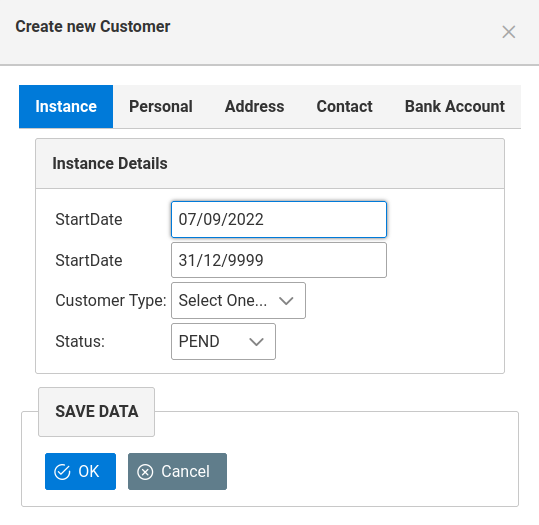
\includegraphics[width=0.50\textwidth]{imaxes/formulario-alta-cliente.png}
  \caption{Detalle del formulario de alta de clientes.}
  \label{fig:formulario-alta-cliente}
\end{figure}

Una vez finaliza la introducción de datos se pulsará el botón \emph{OK} que confirma la operación del formulario de creación. Si todo es correcto se registra el cliente en el sistema, se muestra un mensaje con el id del nuevo cliente creado y se muestran los datos del cliente creado la pantalla de visualización de la entidad.

Por defecto la fecha de Activación del cliente no se cubre, por lo que si queremos activar el cliente deberemos especificarla manualmente a través de la edición del registro del cliente creado.


\begin{figure}[H]
  \centering
  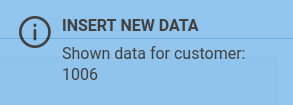
\includegraphics[width=0.3\textwidth]{imaxes/mensaje-id-cliente.png}
  \caption{Detalle del mensaje que informa del id del cliente creado.}
  \label{fig:mensaje-id-cliente}
\end{figure}


\item[\underline{\textsl{\textbf{Editar registro de histórico de cliente}}}] Esta operación sólo está disponible para usuarios con permisos de edición.
Para editar un registro de histórico se seleccionará el registro deseado del listado de históricos de la entidad y se pulsará el botón editar de la columna \textit{EDIT ROW} correspondiente. Se editarán los campos pertinentes directamente en la tabla para realizar las modificaciones oportunas teniendo en cuenta los criterios de fechas establecidos (definidos en la sección \ref{sub:histórico-conceptos} de la página \pageref{sub:histórico-conceptos}).

Al igual que para las entidades con históricos vistas en la sección del catálogo del sistema, si se cambia el estado de un cliente a cancelado, este cambio de estado se propagará a todos los registros posteriores al que cambiamos. Además se establecerá como fecha de cancelación la fecha en la que se realiza dicho cambio, propagándose ese dato por todos los registros de histórico del cliente, no sólo los que están a continuación del registro al que se le cambió el estado a cancelado.

Esta propagación de la fecha de cancelación por todos los registros del histórico  también ocurre si se modifica dicha fecha. Lo mismo ocurre si se cambia la fecha de activación del cliente.

\item[\underline{\textsl{\textbf{Añadir registro de histórico a un cliente}}}] Esta operación sólo está disponible para usuarios con permisos de edición.
Para añadir un nuevo registro de histórico sobre el cliente se seleccionará del listado el registro en el que se ubicará el nuevo registro a añadir y se pulsará el botón añadir de la columna \textit{ADD ROW} correspondiente. Aparecerá una nueva ventana emergente como la que se muestra en la operación de creación pero con los campos cubiertos con la información del registro sobre el que se va a añadir el nuevo registro y se realizarán las modificaciones oportunas sobre los mismos teniendo en cuenta los criterios de fechas establecidos (definidos en la sección \ref{sub:histórico-conceptos} de la página \pageref{sub:histórico-conceptos}).


\item[\underline{\textsl{\textbf{Borrar registro de histórico del cliente }}}] Esta operación sólo está disponible para usuarios con permisos de edición.
Para borrar un registro de histórico del cliente se seleccionará del listado el registro a borrar y se pulsará el botón amarillo de borrar de la columna \textit{DEL ROW} correspondiente.

\item[\underline{\textsl{\textbf{Borrar el cliente}}}]
Esta operación sólo está disponible para usuarios con permisos de edición.
Para borrar completamente un cliente se deben borrar uno a uno todos los registros de histórico del cliente según lo indicado en el punto anterior.
\end{description}


\subsection{Contract - Contrato}
\label{sub:contract}


Esta vista muestra la información relativa a los contratos del sistema.

Toda contratación debe llevar asociada un contrato, Dicho contacto debe ser único. Por lo general este contrato se va a generar en el momento de crear una cuenta, y por lo tanto su generación va a ser automática durante la creación de las cuentas (ver \ref{sub:account}). Sin embargo es posible que necesitemos gestionar datos relativos a la fecha de los contratos.

Un tipo de contrato viene definido por los elementos indicados en la \tablename~\ref{tab:contrato}:



\begin{table}[H]
  \centering
  \rowcolors{2}{white}{udcgray!25}
  \setlength{\leftmargini}{0.4cm}
  \resizebox{14cm}{!} {
  \begin{tabular}{|m{3cm} m{11cm}|}
  \rowcolor{udcpink!25}
  \hline
  	\textbf{Elemento} & \textbf{Descripción} \\\hline
	\textbf{CONTRACT NUMBER} & Número de contrato. Es único y se genera de forma automática.   \\
	\textbf{CREATE DATE} & Es la fecha en la que se crea el contrato. Se genera de forma automática. \\
	\textbf{SEND DATE} & Fecha de envío del contrato al cliente. Por defecto su valor es nulo (se cubrirá cuando se envíe dicho contrato. En esta versión la gestión de este valor debe ser manual). \\		
	\textbf{SIGNED DATE} & Fecha de firma del contrato por el cliente. Por defecto su valor es nulo (se cubrirá cuando se reciba la firma de dicho contrato. En esta versión la gestión de este valor debe ser manual). \\	
	\textbf{ACTIVE DATE} & Fecha de activación del contrato. Por defecto su valor es nulo (se cubrirá cuando se realice la activación de dicho contrato. En esta versión la gestión de este valor debe ser manual). \\	
	\\\hline
  \end{tabular}
  } % end /resizebox
  \caption{Datos que definen un contrato.}
  \label{tab:contrato}
\end{table}

Las operaciones definidas para esta entidad son las siguientes (nota: sólo están habilitadas para usuarios con permisos de edición):
\begin{description}
\item[\underline{\textsl{\textbf{Crear nuevo contrato}}}] Para crear un nuevo contrato se pulsará el botón \textit{New Data} situado en la parte superior de la tabla. Aparecerá una ventana emergente que mostrará un formulario con los campos a cubrir. Si no se establece ningún campo se tomarán los valores por defecto.

\item[\underline{\textsl{\textbf{Editar contrato existente}}}] Para editar un contrato existente se seleccionará del listado y se pulsará el botón editar de la columna \textit{EDIT ROW} correspondiente. Se editarán los campos pertinentes directamente en la tabla para realizar las modificaciones oportunas. 

\item[\underline{\textsl{\textbf{Borrar contrato}}}] Para borrar un contrato se seleccionará del listado y se pulsará el botón amarillo de borrar de la columna \textit{DEL ROW} correspondiente.
\end{description}





\subsubsection{Account - Cuenta}
\label{sub:account}

Esta vista muestra la información relativa a las cuenta contenidas en la cartera de cuentas de la empresa.

Una cuenta depende de un cliente, por lo que existe una relación directa entre una cuenta y su cliente, no puede existir de forma independiente. Puesto que la cuenta es la entidad del sistema que permite gestionar los distintos productos y servicios contratados por el cliente y es la responsable de la transacción económica asociada a la contratación, esto es, el \textit{pagador}, tendrá asociada una persona física o jurídica que es la que efectuará el pago y que puede coincidir con el cliente o ser otra distinta. Por lo tanto el ciclo de facturación que aplicará sobre los distintos elementos contratados vendrá dado por la cuenta asociada a los mismos y vendrá dado por el tipo de cuenta asociado a la misma.


La \tablename~\ref{tab:cuenta} recoge los elementos más relevantes en la definición de una cuenta.
Las operaciones definidas para esta entidad son las siguientes:

\begin{table}
  \centering
  \rowcolors{2}{white}{udcgray!25}
  \setlength{\leftmargini}{0.4cm}
  \resizebox{14cm}{!} {
  \begin{tabular}{|m{5cm} m{9cm}|}
  \rowcolor{udcpink!25}
  \hline
  	\textbf{Elemento} & \textbf{Descripción} \\\hline
  	\textbf{START DATE} & Fecha de inicio del período temporal para el que aplican las condiciones especificadas para dicho período.\\
  	\textbf{END DATE} & Fecha de finalización del período temporal para el que aplican las condiciones especificadas para dicho período.\\
	\textbf{CUSTOMER ID} & Identificador unívoco del cliente al que está vinculado la cuenta.\\
	\textbf{ACCOUNT TYPE} & Tipo de cuenta asociado a la cuenta. Define la información relativa a la facturación.\\
	\textbf{ACCOUNT ID} & Identificador unívoco de la cuenta generado por la aplicación.\\
	\textbf{CODE} & Código identificativo de la cuenta dentro del cliente. Sólo puede existir una cuenta con un código por cliente (aunque puede haber más cuentas con el mismo código identificativo para cuentas que pertenecen a distintos clientes).\\
	\textbf{CONTRACT NUMBER} & Número de contrato asociado a la cuenta. No puede haber más de una cuenta distinta con el mismo número de contrato..\\
	\textbf{NAME} & Nombre de la persona física o jurídica asociada a la cuenta.\\
	\textbf{1st SURNAME} & Primer apellido de la persona física o jurídica asociada a la cuenta.\\
	\textbf{2nd SURNAME} & Segundo apellido de la persona física o jurídica asociada a la cuenta.\\
	\textbf{IDENTITY CARD} & Número del documento de identificación de la persona física o jurídica asociada a la cuenta.\\	
	\textbf{ADDRESS}, \textbf{CITY}, \textbf{STATE}, \textbf{POST CODE}, \textbf{COUNTRY}  & Datos relativos a la dirección de de la persona física o jurídica asociada a la cuenta.\\	
	\textbf{CONTACT PHONE} & Número de teléfono de contacto de la persona física o jurídica asociada a la cuenta (no obligatorio).\\
	\textbf{EMAIL} & Dirección de correo electrónico de la persona física o jurídica asociada a la cuenta (no obligatorio).\\
	\textbf{IBAN}, \textbf{BANK ENTITY}, \textbf{BANK BRANCH}, \textbf{BANK CONTROL DIGIT}, \textbf{BANK ACCOUNT NUMBER} & Cuenta corriente de la persona física o jurídica asociada a la cuenta (no obligatorio).\\
	\textbf{ACTIVE DATE} & Fecha de activación de la cuenta. Común a todos los registros de histórico. Sólo cubierta cuando el cuenta se ha activado en el sistema.\\	
	\textbf{CANCELLED DATE} & Fecha de baja de la cuenta. Común a todos los registros de histórico. Sólo cubierta cuando el cuenta ha cursado baja (estado cancelado).	\\
	\textbf{STATUS} & Estado de la cuenta para el histórico actual.	
	\\\hline
  \end{tabular}
  } % end /resizebox
  \caption{Datos que definen un cuenta.}
  \label{tab:cuenta}
\end{table}

\begin{description}
\item[\underline{\textsl{\textbf{Buscar un cuenta existente}}}] Esta operación está disponible para todos los usuarios de la aplicación.
Se define un área de búsqueda en los que se definen los criterios de búsqueda a tener en cuenta:
\begin{itemize}
	\item Área Account Data: en este área se definen los criterios de búsqueda relativos a la propia cuenta:
	\begin{itemize}
		\item Contract Nr: número de contrato asociado a la cuenta.
		\item Account Id: identificador de la cuenta.
		\item Account Identity Card: número del documento de identificación de la cuenta (NIF, NIE\dots).
	\end{itemize}
	\item Área Customer Data: en este área se definen los criterios de búsqueda del cliente del que depende la cuenta.
	\begin{itemize}
		\item Customer Id: identificador del cliente asociado a la cuenta.
		\item Identity Card: número del documento de identificación del cliente asociado a la cuenta (NIF, NIE\dots).
	\end{itemize}
	\item Área Search Date: fecha de referencia de búsqueda. Se obtendrá como resultado el registro de histórico en el que esté comprendida dicha fecha. Este campo es obligatorio para realizar la búsqueda.
\end{itemize}

Una vez cubiertos los criterios indicados se pulsará el botón \emph{Search}, que mostrará un panel emergente con el listado de los registros encontrados. Seleccionaremos el elemento sobre el que queramos operar pulsando el botón amarillo de la columna \emph{Show Historic}. Se mostrará el área de históricos de la entidad con los distintos registros de histórico existentes.


\item[\underline{\textsl{\textbf{Crear nueva cuenta}}}] Esta operación sólo está habilitada para usuarios con permisos de edición.
Para crear una nueva cuenta se pulsará el botón \textit{New Data} situado en el área \emph{Create New Account} en la parte superior derecha de la ventana. Aparecerá una ventana emergente que mostrará un formulario con distintas pestañas relativas a la información a cubrir. A continuación se detallan dichas pestañas:
\begin{enumerate}
\item Pestaña Contract and Customer Data: en este apartado se define tanto el contrato asociado a la cuenta como el cliente del que depende. 
	\begin{itemize}
		\item Área Contract Data: Si queremos usar un contrato ya existente en el servicio introduciremos el número de contrato a relacionar en el campo de texto \emph{Contract Nr}. Si por el contrario queremos asociar un nuevo contrato pulsaremos el botón \emph{New Contract}, que generará un nuevo número de contrato y lo visualizará en el campo de texto \emph{Contract Nr}.
		\item Área Customer Data: Si sabemos el identificador del cliente del que dependerá la cuenta a crear, introduciremos ese valor en el campo \emph{Customer Id}. En caso contrario introduciremos el valor del documento identificativo del cliente a asociar en el área de texto Customer Identity Card y pulsaremos el botón search. Esto mostrará un listado con los clientes cuyo documento identificativo coincida con el introducido, seleccionaremos el cliente deseado y pulsaremos el botón amarillo de la columna \emph{Select} correspondiente a dicho registro. Esto cargará la información del cliente en el área Customer Data.		
	\end{itemize}		
\item Pestaña Instance Details: aquí se define, entre otros, el tipo de cuenta que va a tener asociada esta cuenta. Los campos a definir son los siguientes y son todos obligatorios:
	\begin{itemize}
	\item Start Date: fecha de inicio del registro a crear (fecha desde la que queremos que la cuenta figure como registrado en el sistema). Por defecto aparece la fecha actual.
	\item End Date: fecha de fin del registro a crear. Por defecto aparece la máxima fecha del sistema (31/12/9999). Recomendamos no modificar esta fecha.
	\item Account Type: clasificación del tipo de cuenta con el que se va a dar de alta la nueva cuenta.
	\item Status: por defecto aparece el status pending, con vistas a la provisión, pero se puede seleccionar otro.
	\end{itemize}
\item Pestaña Personal: aquí se define la información relativa a la persona física o jurídica. Los campos a definir son los siguientes y son todos obligatorios:
	\begin{itemize}
	\item Name: nombre de la persona física o jurídica asociada a la cuenta.
	\item 1st Surname: primer apellido de la persona física o jurídica asociada a la cuenta.
	\item 2nd Surname: segundo apellido de la persona física o jurídica asociada a la cuenta.
	\item ID Card Type: tipo de documento de identificación de la persona física o jurídica asociada a la cuenta. Se seleccionará el que corresponda del listado.
	\item ID Card: número del documento de identificación de la persona física o jurídica asociada a la cuenta.
	\end{itemize}
\item Pestaña Address: aquí se define la información relativa a la dirección de la persona física o jurídica asociada a la cuenta a efectos de notificación. Los campos a definir son los siguientes y son todos obligatorios:
	\begin{itemize}
	\item Address: dirección: calle o vía, número, piso, puerta, etc.
	\item Post Code: código postal.
	\item City: Ciudad.
	\item State: Provincia.
	\item Country: País.
	\end{itemize}
\item Pestaña Contact: aquí se define la información de contacto de la persona física o jurídica asociada a la cuenta. Los campos a definir son los siguientes y no son obligatorios:
	\begin{itemize}
	\item Phone: número de teléfono de contacto.
	\item Email: dirección de correo electrónico.
	\end{itemize}
\item Pestaña Bank Account: aquí se define la información de la cuenta corriente de la persona física o jurídica asociada a la cuenta. Los campos a definir son los siguientes y no son obligatorios, pero si se cubren deben cubrirse todos:
	\begin{itemize}
	\item IBAN: número de Iban (4 caracteres alfanuméricos).
	\item Bank Entity: código del banco (4 dígitos).
	\item Bank Branch: código de entidad (4 dígitos).
	\item Bank Control Digit: dígito de control (2 dígitos).
	\item Bank Account Number: número de cuenta (10 dígitos).	
	\end{itemize}	
\end{enumerate}


\begin{figure}[H]
  \centering
  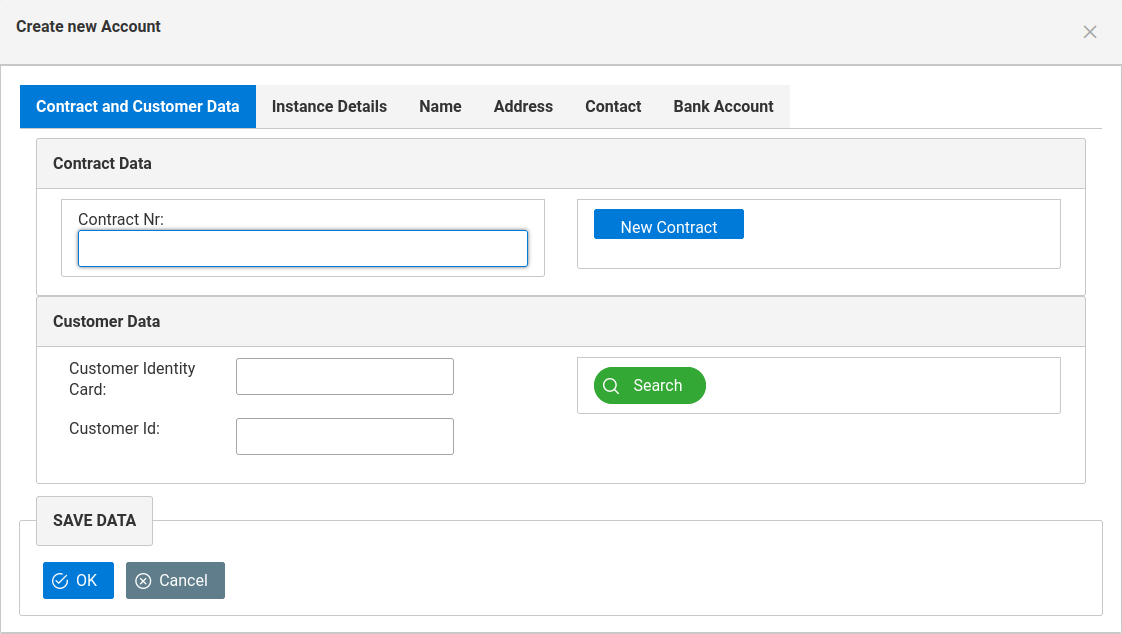
\includegraphics[width=0.9\textwidth]{imaxes/formulario-alta-cuenta.png}
  \caption{Detalle del formulario de alta de cuentas}
  \label{fig:formulario-alta-cuenta}
\end{figure}

Una vez finaliza la introducción de datos se pulsará el botón \emph{OK} que confirma la operación del formulario de creación. Si todo es correcto se registra el cuenta en el sistema, se muestra un mensaje con el id de la nueva cuenta creada y se muestran los datos de la cuenta creado la pantalla de visualización de la entidad.

Por defecto la fecha de Activación de la cuenta no se cubre, por lo que si queremos activar el cuenta deberemos especificarla manualmente a través de la edición del registro de la cuenta creada.


\begin{figure}[H]
  \centering
  
\includegraphics[width=0.35\textwidth]{imaxes/mensaje-id-cuenta.png}
  \caption{Detalle del mensaje que informa del id de la cuenta creado.}
  \label{fig:mensaje-id-cuenta}
\end{figure}


\item[\underline{\textsl{\textbf{Editar registro de histórico de cuenta}}}] Esta operación sólo está disponible para usuarios con permisos de edición.
Para editar un registro de histórico se seleccionará el registro deseado del listado de históricos de la entidad y se pulsará el botón editar de la columna \textit{EDIT ROW} correspondiente. Se editarán los campos pertinentes directamente en la tabla para realizar las modificaciones oportunas teniendo en cuenta los criterios de fechas establecidos (definidos en la sección \ref{sub:histórico-conceptos} de la página \pageref{sub:histórico-conceptos}).

Al igual que para las entidades con históricos vistas en la sección del catálogo del sistema, si se cambia el estado de un cuenta a cancelado, este cambio de estado se propagará a todos los registros posteriores al que cambiamos. Además se establecerá como fecha de cancelación la fecha en la que se realiza dicho cambio, propagándose ese dato por todos los registros de histórico de la cuenta, no sólo los que están a continuación del registro al que se le cambió el estado a cancelado.

Esta propagación de la fecha de cancelación por todos los registros del histórico  también ocurre si se modifica dicha fecha. Lo mismo ocurre si se cambia la fecha de activación de la cuenta.

\item[\underline{\textsl{\textbf{Añadir registro de histórico a un cuenta}}}] Esta operación sólo está disponible para usuarios con permisos de edición.
Para añadir un nuevo registro de histórico sobre el cuenta se seleccionará del listado el registro en el que se ubicará el nuevo registro a añadir y se pulsará el botón añadir de la columna \textit{ADD ROW} correspondiente. Aparecerá una nueva ventana emergente como la que se muestra en la operación de creación  con los campos cubiertos con la información del registro sobre el que se va a añadir el nuevo registro y se realizarán las modificaciones oportunas sobre los mismos teniendo en cuenta los criterios de fechas establecidos (definidos en la sección \ref{sub:histórico-conceptos} de la página \pageref{sub:histórico-conceptos}).


\item[\underline{\textsl{\textbf{Borrar registro de histórico de la cuenta}}}] Esta operación sólo está disponible para usuarios con permisos de edición.
Para borrar un registro de histórico de la cuenta se seleccionará del listado el registro a borrar y se pulsará el botón amarillo de borrar de la columna \textit{DEL ROW} correspondiente.

\item[\underline{\textsl{\textbf{Borrar la cuenta}}}] Esta operación sólo está disponible para usuarios con permisos de edición.
Para borrar completamente un cuenta se deben borrar uno a uno todos los registros de histórico de la cuenta según lo indicado en el punto anterior. 
\end{description}




\subsubsection{Product Instance - Producto}
\label{sub:product}

Esta vista muestra la información relativa a los productos contenidas en la cartera de productos de la empresa.

Un producto es una entidad facturable, por lo que cada instancia del mismo deberá llevar asociado el tipo impositivo asociado según marca la ley. Además el producto debe estar relacionado con una de las cuentas existentes en el sistema, no puede existir de forma independiente.


La \tablename~\ref{tab:producto} recoge los elementos más relevantes en la definición de un producto:

\begin{table}[H]
  \centering
  \rowcolors{2}{white}{udcgray!25}
  \setlength{\leftmargini}{0.4cm}
  \resizebox{14cm}{!} {
  \begin{tabular}{|m{6cm} m{8cm}|}
  \rowcolor{udcpink!25}
  \hline
  	\textbf{Elemento} & \textbf{Descripción} \\\hline
  	\textbf{START DATE} & Fecha de inicio del período temporal para el que aplican las condiciones especificadas para dicho período.\\
  	\textbf{END DATE} & Fecha de finalización del período temporal para el que aplican las condiciones especificadas para dicho período.\\
	\textbf{PRODUCT TYPE} & Tipo de producto asociado al producto.\\
	\textbf{ACCOUNT ID} & Identificador unívoco de la cuenta a la que pertenece el producto.\\
	\textbf{CODE} & Código identificativo del producto. Por defecto es el mismo que el tipo de producto asociado.\\	
	\textbf{TAX TYPE} & Tipo impositivo definido para el producto.\\
	\textbf{ACTIVE DATE} & Fecha de activación del producto. Común a todos los registros de histórico. Sólo cubierta cuando el producto se ha activado en el sistema.\\	
	\textbf{CANCELLED DATE} & Fecha de baja del producto. Común a todos los registros de histórico. Sólo cubierta cuando el producto ha cursado baja (estado cancelado).	\\
	\textbf{STATUS} & Estado del producto para el histórico actual.	
	\\\hline
  \end{tabular}
  } % end /resizebox
  \caption{Datos que definen un producto.}
  \label{tab:producto}
\end{table}



Las operaciones definidas para esta entidad son las siguientes:

\begin{description}
\item[\underline{\textsl{\textbf{Buscar un producto existente}}}] Esta operación está disponible para todos los usuarios de la aplicación.
Se define un área de búsqueda en los que se definen los criterios de búsqueda a tener en cuenta:
\begin{itemize}
	\item Área Account Data: en este área se definen los criterios de búsqueda relativos a la cuenta a la que está asociado el producto:
	\begin{itemize}
		\item Contract Nr: número de contrato asociado a la cuenta.
		\item Account Id: identificador de la cuenta.
		\item Account Identity Card: número del documento de identificación de la cuenta (NIF, NIE\dots).
	\end{itemize}
	\item Área Customer Data: en este área se definen los criterios de búsqueda del cliente del que depende la cuenta asociada al producto.
	\begin{itemize}
		\item Customer Id: identificador del cliente asociado a la cuenta.
		\item Identity Card: número del documento de identificación del cliente asociado a la cuenta (NIF, NIE\dots).
	\end{itemize}
	\item Área Search Date: fecha de referencia de búsqueda. Se obtendrá como resultado el registro de histórico en el que esté comprendida dicha fecha. Este campo es obligatorio para realizar la búsqueda.
\end{itemize}

Una vez cubiertos los criterios indicados se pulsará el botón \emph{Search}, que mostrará un panel emergente con el listado de los registros encontrados. Seleccionaremos el elemento sobre el que queramos operar pulsando el botón amarillo de la columna \emph{Show Historic}. Se mostrará el área de históricos de la entidad con los distintos registros de histórico existentes.


\item[\underline{\textsl{\textbf{Crear nueva producto}}}] Esta operación sólo está habilitada para usuarios con permisos de edición.
Para crear una nueva producto se pulsará el botón \textit{New Data} situado en el área \emph{Create New Product} en la parte superior derecha de la ventana. Aparecerá una ventana emergente que mostrará dos partes diferenciadas. Un área superior denominada \emph{Parent Data} correspondiente a la cuenta asociada al producto y una parte inferior que se corresponde con los datos de la instancia del producto.

Si sabemos el id de la cuenta a la que vamos a asociar el producto la especificaremos en el área de texto \emph{Account Id} del área \emph{Account Criteria} del apartado \emph{Parent Data}. En caso de no saber el id procederemos a cubrir alguno de los campos del formulario del apartado \emph{Parent Data} y pulsaremos el botón \emph{Search}. Aparecerá un listado con todas las cuentas resultado de la búsqueda. Seleccionaremos el registro deseado y pulsaremos el botón amarillo de la columna \emph{Select} correspondiente. Se cargará la información correspondiente en el apartado \emph{Parent Data}.

A continuación cubriremos el resto de los datos correspondientes al producto a crear y que se encuentran debajo del apartado apartado \emph{Parent Data}:
\begin{itemize}
	\item Start Date: fecha de inicio del registro a crear (fecha desde la que queremos que el producto figure como registrado en el sistema). Por defecto aparece la fecha actual.
	\item End Date: fecha de fin del registro a crear. Por defecto aparece la máxima fecha del sistema (31/12/9999). Recomendamos no modificar esta fecha.
	\item Tax Type: Tipo impositivo a aplicar al producto a efectos de facturación.
	\item Product Type: tipo de producto al que pertenece el producto a crear.
	\item Status: por defecto aparece el status pending, con vistas a la provisión, pero se puede seleccionar otro.
\end{itemize}


\begin{figure}[H]
  \centering
  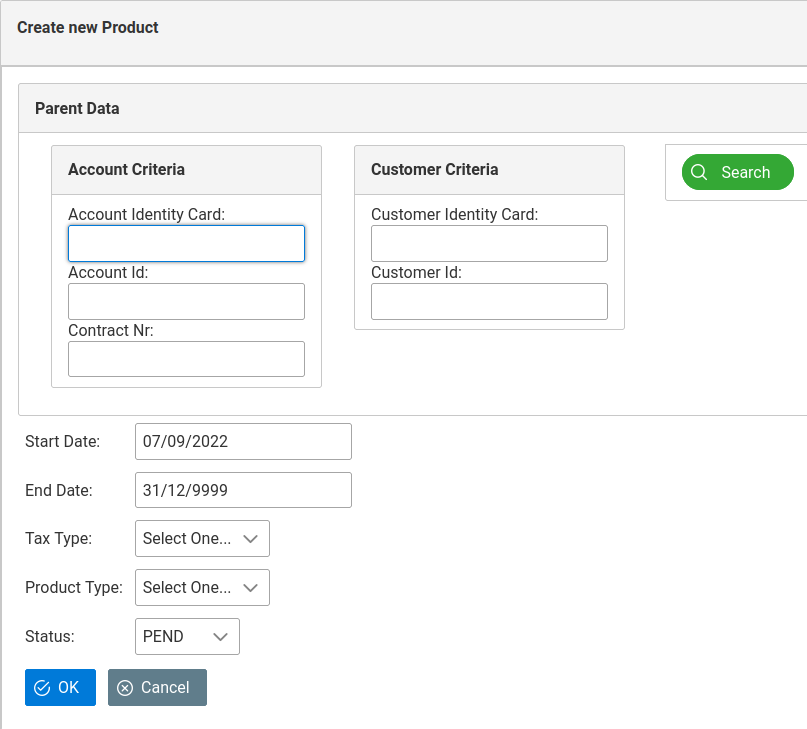
\includegraphics[width=0.70\textwidth]{imaxes/formulario-alta-producto.png}
  \caption{Detalle del formulario de alta de productos}
  \label{fig:formulario-alta-producto}
\end{figure}

Una vez finaliza la introducción de datos se pulsará el botón \emph{OK} que confirma la operación del formulario de creación. Si todo es correcto se registra el producto en el sistema y se muestran los datos del producto creado la pantalla de visualización de la entidad.

Por defecto la fecha de Activación del producto no se cubre, por lo que si queremos activar el producto deberemos especificarla manualmente a través de la edición del registro del producto creada.


\item[\underline{\textsl{\textbf{Editar registro de histórico de producto}}}] Esta operación sólo está disponible para usuarios con permisos de edición.
Para editar un registro de histórico se seleccionará el registro deseado del listado de históricos de la entidad y se pulsará el botón editar de la columna \textit{EDIT ROW} correspondiente. Se editarán los campos pertinentes directamente en la tabla para realizar las modificaciones oportunas teniendo en producto los criterios de fechas establecidos (definidos en la sección \ref{sub:histórico-conceptos} de la página \pageref{sub:histórico-conceptos}).

Al igual que para las entidades con históricos vistas en la sección del catálogo del sistema, si se cambia el estado de un producto a cancelado, este cambio de estado se propagará a todos los registros posteriores al que cambiamos. Además se establecerá como fecha de cancelación la fecha en la que se realiza dicho cambio, propagándose ese dato por todos los registros de histórico del producto, no sólo los que están a continuación del registro al que se le cambió el estado a cancelado.

Esta propagación de la fecha de cancelación por todos los registros del histórico  también ocurre si se modifica dicha fecha. Lo mismo ocurre si se cambia la fecha de activación del producto.

\item[\underline{\textsl{\textbf{Añadir registro de histórico a un producto}}}] Esta operación sólo está disponible para usuarios con permisos de edición.
Para añadir un nuevo registro de histórico sobre el producto se seleccionará del listado el registro en el que se ubicará el nuevo registro a añadir y se pulsará el botón añadir de la columna \textit{ADD ROW} correspondiente. Aparecerá una nueva ventana emergente como la que se muestra en la operación de creación sin el área de búsqueda \emph{Parent Data} y con los campos cubiertos con la información del registro sobre el que se va a añadir el nuevo registro y se realizarán las modificaciones oportunas sobre los mismos teniendo en servicio los criterios de fechas establecidos (definidos en la sección \ref{sub:histórico-conceptos} de la página \pageref{sub:histórico-conceptos}). En la \figurename~\ref{fig:nuevo-historico-producto} se puede ver un detalle del formulario correspondiente.

\begin{figure}
  \centering
  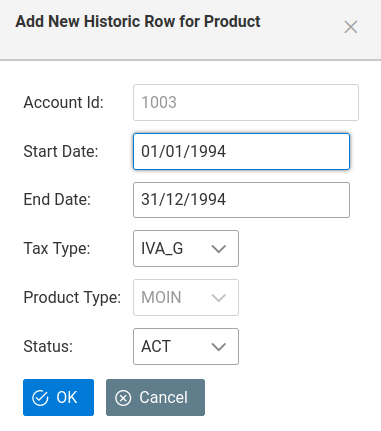
\includegraphics[width=0.4\textwidth]{imaxes/nuevo-historico-producto.png}
  \caption{Detalle del formulario para añadir un nuevo registro de histórico de producto}
  \label{fig:nuevo-historico-producto}
\end{figure}


\item[\underline{\textsl{\textbf{Borrar registro de histórico del producto}}}] Esta operación sólo está disponible para usuarios con permisos de edición.
Para borrar un registro de histórico del producto se seleccionará del listado el registro a borrar y se pulsará el botón amarillo de borrar de la columna \textit{DEL ROW} correspondiente.

\item[\underline{\textsl{\textbf{Borrar el producto}}}] Esta operación sólo está disponible para usuarios con permisos de edición.
Para borrar completamente un producto se deben borrar uno a uno todos los registros de histórico del producto según lo indicado en el punto anterior. 
\end{description}


\subsubsection{Service Instance - Servicio}
\label{sub:service}

Esta vista muestra la información relativa a los servicios contenidas en la cartera de servicios de la empresa.

Un servicio es una entidad facturable, por lo que cada instancia del mismo deberá llevar asociado el tipo impositivo asociado según marca la ley. Además un servicio debe estar asociado a uno de los productos existentes en el sistema, no puede existir de forma independiente.

\begin{table}
  \centering
  \rowcolors{2}{white}{udcgray!25}
  \setlength{\leftmargini}{0.4cm}
  \resizebox{14cm}{!} {
  \begin{tabular}{|m{4.5cm} m{11cm}|}
  \rowcolor{udcpink!25}
  \hline
  	\textbf{Elemento} & \textbf{Descripción} \\\hline
  	\textbf{START DATE} & Fecha de inicio del período temporal para el que aplican las condiciones especificadas para dicho período.\\
  	\textbf{END DATE} & Fecha de finalización del período temporal para el que aplican las condiciones especificadas para dicho período.\\
	\textbf{PRODUCT ID} & Identificador unívoco del producto al que está vinculado el servicio.\\
	\textbf{SERVICE TYPE} & Tipo de servicio asociado al servicio.\\
	\textbf{SERVICE NUMBER} & Número que identifica al servicio. Sólo debe existir un servicio con estado distinto de cancelado en el sistema con ese número.\\
	\textbf{GENERAL 1}, \textbf{GENERAL 2}, \textbf{GENERAL 3} & Campos generales que contienen información adicional del servicio (no definidos).\\	
	\textbf{TAX TYPE} & Tipo impositivo definido para el servicio.\\
	\textbf{ACTIVE DATE} & Fecha de activación del servicio. Común a todos los registros de histórico. Sólo cubierta cuando el servicio se ha activado en el sistema.\\	
	\textbf{CANCELLED DATE} & Fecha de baja del servicio. Común a todos los registros de histórico. Sólo cubierta cuando el servicio ha cursado baja (estado cancelado).	\\
	\textbf{STATUS} & Estado del servicio para el histórico actual.	
	\\\hline
  \end{tabular}
  } % end /resizebox
  \caption{Datos que definen un servicio.}
  \label{tab:servicio}
\end{table}

La \tablename~\ref{tab:servicio} recoge los elementos más relevantes en la definición de un servicio.
Las operaciones definidas para esta entidad son las siguientes:
\begin{description}
\item[\underline{\textsl{\textbf{Buscar un servicio existente}}}] Esta operación está disponible para todos los usuarios de la aplicación.
Se define un área de búsqueda en los que se definen los criterios de búsqueda a tener en cuenta:
\begin{itemize}
	\item Área Account Data: en este área se definen los criterios de búsqueda relativos a la cuenta a la que está asociado el servicio:
		\begin{itemize}
			\item Contract Nr: número de contrato asociado a la cuenta.
			\item Account Id: identificador de la cuenta.
			\item Account Identity Card: número del documento de identificación de la cuenta (NIF, NIE\dots).
		\end{itemize}
	\item Área Customer Data: en este área se definen los criterios de búsqueda del cliente del que depende la cuenta asociada al servicio.
		\begin{itemize}
			\item Customer Id: identificador del cliente asociado a la cuenta.
			\item Identity Card: número del documento de identificación del cliente asociado a la cuenta (NIF, NIE\dots).
		\end{itemize}
	\item Área Product Data: en este área se definen los criterios de búsqueda del producto del que depende el servicio. Está pensada para completar la búsqueda con otra información aportada en el resto de áreas.	
		\begin{itemize}
			\item Product Id: identificador del producto.
			\item Product Type: tipo del producto.
		\end{itemize}
	\item Área Service Data: en este área se definen los criterios de búsqueda del servicio.
		\begin{itemize}
			\item Service Nr: número del servicio a buscar.
			\item Product Type: tipo del servicio a buscar. Está pensada para completar la búsqueda con otra información aportada en el resto de áreas.
		\end{itemize}
	\item Área Search Date: fecha de referencia de búsqueda. Se obtendrá como resultado el registro de histórico en el que esté comprendida dicha fecha. Este campo es obligatorio para realizar la búsqueda.
\end{itemize}

Una vez cubiertos los criterios indicados se pulsará el botón \emph{Search}, que mostrará un panel emergente con el listado de los registros encontrados. Seleccionaremos el elemento sobre el que queramos operar pulsando el botón amarillo de la columna \emph{Show Historic}. Se mostrará el área de históricos de la entidad con los distintos registros de histórico existentes.

\item[\underline{\textsl{\textbf{Crear nueva servicio}}}] Esta operación sólo está habilitada para usuarios con permisos de edición.
Para crear una nueva servicio se pulsará el botón \textit{New Data} situado en el área \emph{Create New Service} en la parte superior derecha de la ventana. Aparecerá una ventana emergente que mostrará dos partes diferenciadas. Un área superior denominada \emph{Parent Data} correspondiente al producto asociado al servicio y una parte inferior que se corresponde con los datos de la instancia del servicio.

Si sabemos el id del producto a la que vamos a asociar el servicio la especificaremos en el área de texto \emph{Product Id} del área \emph{Product Criteria} del apartado \emph{Parent Data}. En caso de no saber el id procederemos a cubrir alguno de los campos del formulario del apartado \emph{Parent Data} de forma análoga a lo realizado para especificar los criterios de búsqueda del servicio y pulsaremos el botón \emph{Search}. Aparecerá un listado con todos los productos resultado de la búsqueda. Seleccionaremos el registro deseado y pulsaremos el botón amarillo de la columna \emph{Select} correspondiente. Se cargará la información correspondiente en el apartado \emph{Parent Data}.

A continuación cubriremos el resto de los datos correspondientes al servicio a crear y que se encuentran debajo del apartado apartado \emph{Parent Data}:
\begin{itemize}
	\item Start Date: fecha de inicio del registro a crear (fecha desde la que queremos que el servicio figure como registrado en el sistema). Por defecto aparece la fecha actual.
	\item End Date: fecha de fin del registro a crear. Por defecto aparece la máxima fecha del sistema (31/12/9999). Recomendamos no modificar esta fecha.
	\item Tax Type: Tipo impositivo a aplicar al servicio a efectos de facturación.
	\item Service Type: tipo de servicio al que pertenece el servicio a crear.	
		\item Fee Type: tipo de servicio a crear. 
	\item General 1: campo reservado a información adicional. Puede dejarse sin cubrir.
	\item General 2: campo reservado a información adicional. Puede dejarse sin cubrir.
	\item General 3: campo reservado a información adicional. Puede dejarse sin cubrir.
	\item Status: por defecto aparece el status pending, con vistas a la provisión, pero se puede seleccionar otro.
\end{itemize}

Una vez finaliza la introducción de datos se pulsará el botón \emph{OK} que confirma la operación del formulario de creación. Si todo es correcto se registra el servicio en el sistema y se muestran los datos del servicio creado la pantalla de visualización de la entidad.

Por defecto la fecha de Activación del servicio no se cubre, por lo que si queremos activar el servicio deberemos especificarla manualmente a través de la edición del registro del servicio creada.

La \figurename~\ref{fig:formulario-alta-servicio} muestra un detalle del formulario de alta de servicios.

\begin{figure}
  \centering
  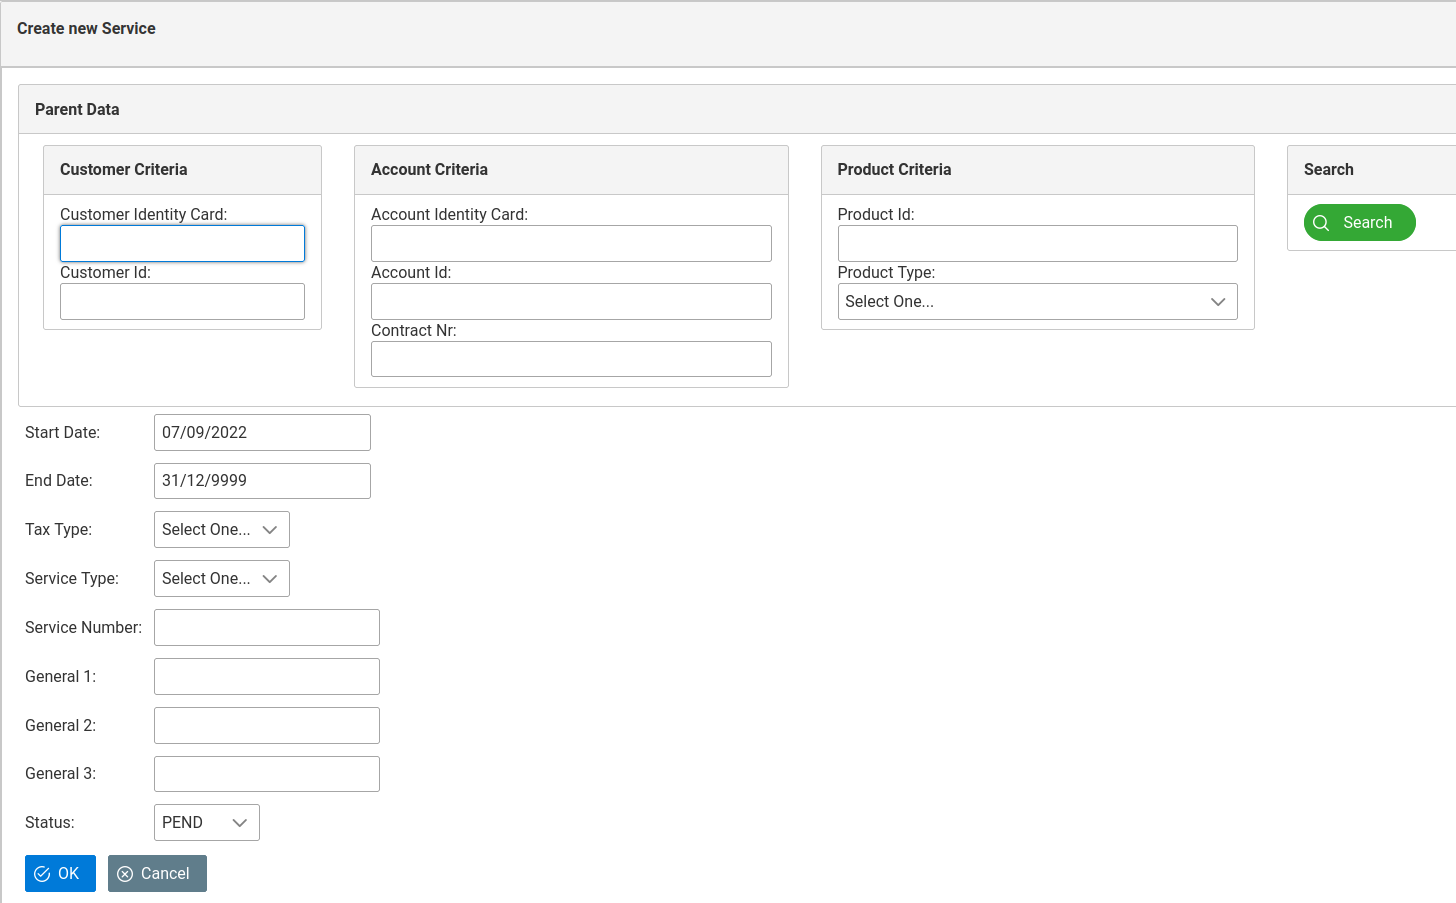
\includegraphics[width=0.9\textwidth]{imaxes/formulario-alta-servicio.png}
  \caption{Detalle del formulario de alta de servicios}
  \label{fig:formulario-alta-servicio}
\end{figure}


\item[\underline{\textsl{\textbf{Editar registro de histórico de servicio}}}] Esta operación sólo está disponible para usuarios con permisos de edición.
Para editar un registro de histórico se seleccionará el registro deseado del listado de históricos de la entidad y se pulsará el botón editar de la columna \textit{EDIT ROW} correspondiente. Se editarán los campos pertinentes directamente en la tabla para realizar las modificaciones oportunas teniendo en servicio los criterios de fechas establecidos (definidos en la sección \ref{sub:histórico-conceptos} de la página \pageref{sub:histórico-conceptos}).

Al igual que para las entidades con históricos vistas en la sección del catálogo del sistema, si se cambia el estado de un servicio a cancelado, este cambio de estado se propagará a todos los registros posteriores al que cambiamos. Además se establecerá como fecha de cancelación la fecha en la que se realiza dicho cambio, propagándose ese dato por todos los registros de histórico del servicio, no sólo los que están a continuación del registro al que se le cambió el estado a cancelado.

Esta propagación de la fecha de cancelación por todos los registros del histórico  también ocurre si se modifica dicha fecha. Lo mismo ocurre si se cambia la fecha de activación del servicio.

\item[\underline{\textsl{\textbf{Añadir registro de histórico a un servicio}}}] Esta operación sólo está disponible para usuarios con permisos de edición.
Para añadir un nuevo registro de histórico sobre el servicio se seleccionará del listado el registro en el que se ubicará el nuevo registro a añadir y se pulsará el botón añadir de la columna \textit{ADD ROW} correspondiente. Aparecerá una nueva ventana emergente como la que se muestra en la operación de creación sin el área de búsqueda \emph{Parent Data} y con los campos cubiertos con la información del registro sobre el que se va a añadir el nuevo registro y se realizarán las modificaciones oportunas sobre los mismos teniendo en servicio los criterios de fechas establecidos (definidos en la sección \ref{sub:histórico-conceptos} de la página \pageref{sub:histórico-conceptos}).

La \figurename~\ref{fig:nuevo-historico-servicio} muestra un detalle del formulario para añadir un nuevo registro al histórico de un servicio:

\begin{figure}[H]
  \centering
  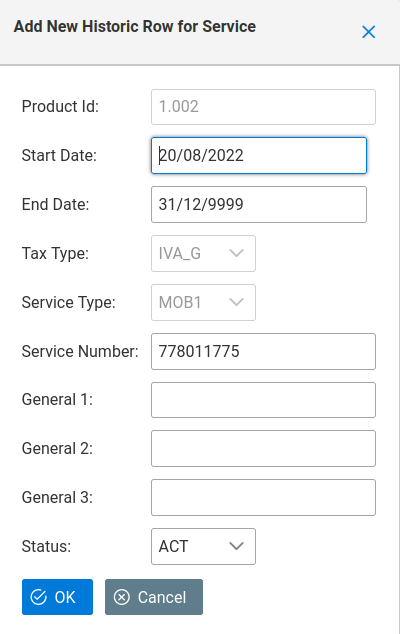
\includegraphics[width=0.40\textwidth]{imaxes/nuevo-historico-servicio.png}
  \caption{Detalle del formulario para añadir un nuevo registro de histórico de servicio}
  \label{fig:nuevo-historico-servicio}
\end{figure}


\item[\underline{\textsl{\textbf{Borrar registro de histórico del servicio}}}] Esta operación sólo está disponible para usuarios con permisos de edición.
Para borrar un registro de histórico del servicio se seleccionará del listado el registro a borrar y se pulsará el botón amarillo de borrar de la columna \textit{DEL ROW} correspondiente.

\item[\underline{\textsl{\textbf{Borrar el servicio}}}] Esta operación sólo está disponible para usuarios con permisos de edición.
Para borrar completamente un servicio se deben borrar uno a uno todos los registros de histórico del servicio según lo indicado en el punto anterior. 
\end{description}


\subsubsection{Fee Instance - Cuota}
\label{sub:fee}

Esta vista muestra la información relativa a las cuotas contenidas en la cartera de servicios de la empresa.

Una cuota debe estar asociado a un producto o servicio existentes en el sistema, no puede existir de forma independiente.

Aunque los valores de prorrateo y precio de la cuota vienen definidos por el tipo de cuota asociado a la cuota contratada, estos valores pueden cambiar en la cuota, para adaptarse a las necesidades del cliente.

La \tablename~\ref{tab:cuota} recoge los elementos más relevantes en la definición de una cuota.
Las operaciones definidas para esta entidad son las siguientes.

\begin{table}
  \centering
  \rowcolors{2}{white}{udcgray!25}
  \setlength{\leftmargini}{0.4cm}
  \resizebox{14cm}{!} {
  \begin{tabular}{|m{4cm} m{11cm}|}
  \rowcolor{udcpink!25}
  \hline
  	\textbf{Elemento} & \textbf{Descripción} \\\hline
  	\textbf{START DATE} & Fecha de inicio del período temporal para el que aplican las condiciones especificadas para dicho período.\\
  	\textbf{END DATE} & Fecha de finalización del período temporal para el que aplican las condiciones especificadas para dicho período.\\
	\textbf{PARENT ID} & Identificador unívoco de la instancia a la que está vinculada la cuota (product\_id si la cuota aplica a nivel de producto o service\_id si aplica a nivel de servicio).\\
	\textbf{CODE} & Código identificativo de la cuota. Por defecto es el mismo que el tipo de cuota asociado.\\	
	\textbf{FEE TYPE} & Tipo de cuota asociado a la cuota.\\
	\textbf{APPLICATION LEVEL} & Nivel de aplicación de la cuota (producto o servicio). Viene dado por su tipo de cuota.\\
	\textbf{PRORRATE} & Indica si la cuota es prorrateable (\textit{TRUE}) o no (\textit{FALSE}). Se toma como base el importe definido en el tipo de cuota, pero puede variar para adaptarse a las necesidades del cliente.\\
	\textbf{PRICE} & Indica el importe a facturar por dicha cuota. Se toma como base el importe definido en el tipo de cuota, pero puede variar para adaptarse a las necesidades del cliente.\\
	\textbf{ACTIVE DATE} & Fecha de activación de la cuota. Común a todos los registros de histórico. Sólo cubierta cuando la cuota se ha activado en el sistema.\\
	\textbf{CANCELLED DATE} & Fecha de baja de la cuota. Común a todos los registros de histórico. Sólo cubierta cuando la cuota ha cursado baja (estado cancelado).\\
	\textbf{STATUS} & Estado de la cuota para el histórico actual.	
	\\\hline
  \end{tabular}
  } % end /resizebox
  \caption{Datos que definen una cuota.}
  \label{tab:cuota}
\end{table}

\begin{description}
\item[\underline{\textsl{\textbf{Buscar una cuota existente}}}] Esta operación está disponible para todos los usuarios de la aplicación.
Se define un área de búsqueda en los que se definen los criterios de búsqueda a tener en cuenta:
\begin{itemize}
	\item Área Account Data: en este área se definen los criterios de búsqueda relativos a la cuenta a la que está asociada la cuota:
		\begin{itemize}
			\item Contract Nr: número de contrato asociado a la cuenta.
			\item Account Id: identificador de la cuenta.
			\item Account Identity Card: número del documento de identificación de la cuenta (NIF, NIE\dots).
		\end{itemize}
	\item Área Customer Data: en este área se definen los criterios de búsqueda del cliente del que depende la cuenta asociada a la cuota.
		\begin{itemize}
			\item Customer Id: identificador del cliente asociado a la cuenta.
			\item Identity Card: número del documento de identificación del cliente asociado a la cuenta (NIF, NIE\dots).
		\end{itemize}
	\item Área Paren Instance: en este área se definen los criterios de búsqueda de la entidad padre de la cuota. Para ello se selecciona el nivel de aplicación de la cuota a buscar. Se puede completar la búsqueda aportando información relativa a la entidad padre a la que está asociada la cuenta, para lo que se definen unos campos a cubrir. En función de si se ha seleccionado producto o servicio se muestran distintos campos:
	\begin{itemize}
 		\item \emph{Application Level: PRODUCTO} seleccionado: se mostrarán los siguientes campos a cubrir:
			\begin{itemize}
				\item Product Id: identificador del producto al que está asociado la cuota.
				\item Product Type: tipo del producto al que está asociado la cuota.
			\end{itemize}
		\item \emph{Application Level: SERVICE} seleccionado:  se mostrarán los siguientes campos a cubrir:
		\begin{itemize}
			\item Service Nr: número de servicio del servicio al que está asociado la cuota.
			\item Product Type: tipo de servicio del servicio al que está asociado la cuota.
		\end{itemize}
		
	\end{itemize}	    	
	\item Área Search Date: fecha de referencia de búsqueda. Se obtendrá como resultado el registro de histórico en el que esté comprendida dicha fecha. Este campo es obligatorio para realizar la búsqueda.
\end{itemize}

Una vez cubiertos los criterios indicados se pulsará el botón \emph{Search}, que mostrará un panel emergente con el listado de los registros encontrados para las cuotas que cumplan los criterios de búsqueda especificados. Seleccionaremos el elemento sobre el que queramos operar pulsando el botón amarillo de la columna \emph{Show Historic}. Se mostrará el área de históricos de la entidad con los distintos registros de histórico existentes.


\item[\underline{\textsl{\textbf{Crear nueva cuota}}}] Esta operación sólo está habilitada para usuarios con permisos de edición.
Para crear una nueva servicio se pulsará el botón \textit{New Data} situado en el área \emph{Create New Fee} en la parte superior derecha de la ventana. Aparecerá una ventana emergente que mostrará dos partes diferenciadas. Un área superior denominada \emph{Search Parent Data} minimizada correspondiente a la jerarquía de la entidad producto o servicio asociada a la cuota a crear y una parte inferior que se corresponde con los datos de la instancia de la cuota.

Si sabemos el id de la entidad a la que vamos a asociar la cuota la especificaremos en el área de texto \emph{Parent Id}. En caso de no saber el id procederemos a realizar la correspondiente búsqueda en el área  \emph{Search Parent Data}. Para ello desplegaremos ese área pulsando sobre \emph{Search Parent Data} y procederemos a cubrir alguno de los campos del formulario del apartado \emph{Search Parent Data} de forma análoga a lo realizado para especificar los criterios de búsqueda de la cuota y pulsaremos el botón \emph{Search}. Aparecerá un listado con todos los productos o servicios (en función del nivel de aplicación seleccionado) resultado de la búsqueda. Seleccionaremos el registro deseado y pulsaremos el botón amarillo de la columna \emph{Select} correspondiente. Se cargará la información correspondiente en el apartado \emph{Search Parent Data}, así como los datos de \emph{Application Level} y \emph{Parent Id} del área de datos de la instancia de la cuota a crear.

A continuación cubriremos el resto de los datos correspondientes a la cuota a crear y que se encuentran debajo del apartado \emph{Search Parent Data} (importante: si el apartado \emph{Search Parent Data} está desplegado es posible que no se vea todo el formulario de creación de la cuota, por lo que habrá que minimizarlo pulsando en el nombre del apartado (\emph{Search Parent Data})).
\begin{itemize}
	\item Start Date: fecha de inicio del registro a crear (fecha desde la que queremos que la cuota figure como registrado en el sistema). Por defecto aparece la fecha actual.
	\item End Date: fecha de fin del registro a crear. Por defecto aparece la máxima fecha del sistema (31/12/9999). Recomendamos no modificar esta fecha.
	\item Application Level Id: Nivel de aplicación de la cuota. Si se ha recurrido al apartado \emph{Search Parent Data} del formulario para buscar la entidad con la que se va a relacionar la cuota, este campo se cubrirá de forma automática. 
	\item Parent Id: Identificador de la entidad padre a asociar la cuota. Si se ha recurrido al apartado \emph{Search Parent Data} del formulario para buscar la entidad con la que se va a relacionar la cuota, este campo se cubrirá de forma automática. 
	\item Fee Type: tipo de servicio a crear. La información mostrada en el desplegable se cubre en función de los datos del nivel de aplicación y del tipo asociado al Parent Id especificado y viene determinado por las relaciones de tipos de cuota establecidas en el catálogo de servicio para el tipo de entidad padre de la cuota a crear.
	\item Code: código asociado a la cuota.
	\item Prorrate: define si la cuota a crear será prorrateable (\textit{TRUE}) o no (\textit{FALSE}).
	\item Price: precio de la cuota a crear.
	\item Status: por defecto aparece el status pending, con vistas a la provisión, pero se puede seleccionar otro.
\end{itemize}



\begin{figure}
  \centering
  \begin{subfigure}[b]{0.3\textwidth}
    \includegraphics[width=\textwidth]{imaxes/formulario-alta-cuota-01.png}
    \caption{Sin el área de \emph{Search Parent Data} desplegada}
    \label{fig:formulario-alta-cuota-01}
  \end{subfigure}
%  \hspace{0.1\textwidth}
  \begin{subfigure}[b]{0.69\textwidth}
    \includegraphics[width=\textwidth,height=3cm]{imaxes/formulario-alta-cuota-02.png}
    \caption{Con el área de \emph{Search Parent Data} desplegada}
    \label{fig:formulario-alta-cuota-02}
  \end{subfigure}
  \caption{Detalles del formulario de alta de cuota}
  \label{fig:alta-cuota}
\end{figure}


Una vez finaliza la introducción de datos se pulsará el botón \emph{OK} que confirma la operación del formulario de creación. Si todo es correcto se registra la cuota en el sistema y se muestran los datos de la cuota creado la pantalla de visualización de la entidad.

Por defecto la fecha de Activación de la cuota no se cubre, por lo que si queremos activar la cuota deberemos especificarla manualmente a través de la edición del registro de la cuota creada.

La \figurename~\ref{fig:alta-cuota} muestra dos detalles del formulario para añadir una nueva cuota, con y sin el \emph{Search Parent Data} desplegado.

\item[\underline{\textsl{\textbf{Editar registro de histórico de servicio}}}] Esta operación sólo está disponible para usuarios con permisos de edición.
Para editar un registro de histórico se seleccionará el registro deseado del listado de históricos de la entidad y se pulsará el botón editar de la columna \textit{EDIT ROW} correspondiente. Se editarán los campos pertinentes directamente en la tabla para realizar las modificaciones oportunas teniendo en servicio los criterios de fechas establecidos (definidos en la sección \ref{sub:histórico-conceptos} de la página \pageref{sub:histórico-conceptos}).

Al igual que para las entidades con históricos vistas en la sección del catálogo del sistema, si se cambia el estado de una cuota a cancelado, este cambio de estado se propagará a todos los registros posteriores al que cambiamos. Además se establecerá como fecha de cancelación la fecha en la que se realiza dicho cambio, propagándose ese dato por todos los registros de histórico de la cuota, no sólo los que están a continuación del registro al que se le cambió el estado a cancelado.

Esta propagación de la fecha de cancelación por todos los registros del histórico  también ocurre si se modifica dicha fecha. Lo mismo ocurre si se cambia la fecha de activación de la cuota.

\item[\underline{\textsl{\textbf{Añadir registro de histórico a una cuota}}}] Esta operación sólo está disponible para usuarios con permisos de edición.
Para añadir un nuevo registro de histórico sobre la cuota se seleccionará del listado el registro en el que se ubicará el nuevo registro a añadir y se pulsará el botón añadir de la columna \textit{ADD ROW} correspondiente. Aparecerá una nueva ventana emergente como la que se muestra en la operación de creación sin el área de búsqueda \emph{Parent Data} y con los campos cubiertos con la información del registro sobre el que se va a añadir el nuevo registro y se realizarán las modificaciones oportunas sobre los mismos teniendo en servicio los criterios de fechas establecidos (definidos en la sección \ref{sub:histórico-conceptos} de la página \pageref{sub:histórico-conceptos}).

La \figurename~\ref{fig:nuevo-historico-cuota} muestra un detalle del formulario para añadir un nuevo registro al histórico de una cuota

\begin{figure}
  \centering
  \includegraphics[width=0.425\textwidth]{imaxes/nuevo-historico-cuota.png}
  \caption{Detalle del formulario para añadir un nuevo registro de histórico de cuota}
  \label{fig:nuevo-historico-cuota}
\end{figure}



\item[\underline{\textsl{\textbf{Borrar registro de histórico de la cuota}}}] Esta operación sólo está disponible para usuarios con permisos de edición.
Para borrar un registro de histórico de la cuota se seleccionará del listado el registro a borrar y se pulsará el botón amarillo de borrar de la columna \textit{DEL ROW} correspondiente.

\item[\underline{\textsl{\textbf{Borrar la cuota}}}] Esta operación sólo está disponible para usuarios con permisos de edición.
Para borrar completamente una cuota se deben borrar uno a uno todos los registros de histórico de la cuota según lo indicado en el punto anterior. 
\end{description}



\subsubsection{Promotion Instance - Promoción}
\label{sub:promotion}

Esta vista muestra la información relativa a las promociones contenidas en la cartera de servicios de la empresa.

Una promoción debe estar asociado a un producto o servicio existentes en el sistema, no puede existir de forma independiente.

Aunque los valores de prorrateo y precio de la promoción vienen definidos por el tipo de promoción asociado a la promoción contratada, estos valores pueden cambiar en la promoción, para adaptarse a las necesidades del cliente.







Las operaciones definidas para esta entidad son las siguientes:
\begin{description}
\item[\underline{\textsl{\textbf{Buscar una promoción existente}}}] Esta operación está disponible para todos los usuarios de la aplicación.
Se define un área de búsqueda en los que se definen los criterios de búsqueda a tener en cuenta:
\begin{itemize}
	\item Área Account Data: en este área se definen los criterios de búsqueda relativos a la cuenta a la que está asociada la promoción:
		\begin{itemize}
			\item Contract Nr: número de contrato asociado a la cuenta.
			\item Account Id: identificador de la cuenta.
			\item Account Identity Card: número del documento de identificación de la cuenta (NIF, NIE\dots).
		\end{itemize}
	\item Área Customer Data: en este área se definen los criterios de búsqueda del cliente del que depende la cuenta asociada a la promoción.
		\begin{itemize}
			\item Customer Id: identificador del cliente asociado a la cuenta.
			\item Identity Card: número del documento de identificación del cliente asociado a la cuenta (NIF, NIE\dots).
		\end{itemize}
	\item Área Paren Instance: en este área se definen los criterios de búsqueda de la entidad padre de la promoción. Para ello se selecciona el nivel de aplicación de la promoción a buscar. Se puede completar la búsqueda aportando información relativa a la entidad padre a la que está asociada la cuenta, para lo que se definen unos campos a cubrir. En función de si se ha seleccionado producto o servicio se muestran distintos campos:
	\begin{itemize}
 		\item \emph{Application Level: PRODUCTO} seleccionado: se mostrarán los siguientes campos a cubrir:
			\begin{itemize}
				\item Product Id: identificador del producto al que está asociado la promoción.
				\item Product Type: tipo del producto al que está asociado la promoción.
			\end{itemize}
		\item \emph{Application Level: SERVICE} seleccionado:  se mostrarán los siguientes campos a cubrir:
		\begin{itemize}
			\item Service Nr: número de servicio del servicio al que está asociado la promoción.
			\item Product Type: tipo de servicio del servicio al que está asociado la promoción.
		\end{itemize}
		
	\end{itemize}	    	
	\item Área Search Date: fecha de referencia de búsqueda. Se obtendrá como resultado el registro de histórico en el que esté comprendida dicha fecha. Este campo es obligatorio para realizar la búsqueda.
\end{itemize}

Una vez cubiertos los criterios indicados se pulsará el botón \emph{Search}, que mostrará un panel emergente con el listado de los registros encontrados para las promociones que cumplan los criterios de búsqueda especificados. Seleccionaremos el elemento sobre el que queramos operar pulsando el botón amarillo de la columna \emph{Show Historic}. Se mostrará el área de históricos de la entidad con los distintos registros de histórico existentes.


\item[\underline{\textsl{\textbf{Crear nueva promoción}}}] Esta operación sólo está habilitada para usuarios con permisos de edición.
Para crear una nueva servicio se pulsará el botón \textit{New Data} situado en el área \emph{Create New Fee} en la parte superior derecha de la ventana. Aparecerá una ventana emergente que mostrará dos partes diferenciadas. Un área superior denominada \emph{Search Parent Data} minimizada correspondiente a la jerarquía de la entidad producto o servicio asociada a la promoción a crear y una parte inferior que se corresponde con los datos de la instancia de la promoción.

Si sabemos el id de la entidad a la que vamos a asociar la promoción la especificaremos en el área de texto \emph{Parent Id}. En caso de no saber el id procederemos a realizar la correspondiente búsqueda en el área  \emph{Search Parent Data}. Para ello desplegaremos ese área pulsando sobre \emph{Search Parent Data} y procederemos a cubrir alguno de los campos del formulario del apartado \emph{Search Parent Data} de forma análoga a lo realizado para especificar los criterios de búsqueda de la promoción y pulsaremos el botón \emph{Search}. Aparecerá un listado con todos los productos o servicios (en función del nivel de aplicación seleccionado) resultado de la búsqueda. Seleccionaremos el registro deseado y pulsaremos el botón amarillo de la columna \emph{Select} correspondiente. Se cargará la información correspondiente en el apartado \emph{Search Parent Data}, así como los datos de \emph{Application Level} y \emph{Parent Id} del área de datos de la instancia de la promoción a crear.

A continuación cubriremos el resto de los datos correspondientes a la promoción a crear y que se encuentran debajo del apartado \emph{Search Parent Data} (importante: si el apartado \emph{Search Parent Data} está desplegado es posible que no se vea todo el formulario de creación de la promoción, por lo que habrá que minimizarlo pulsando en el nombre del apartado (\emph{Search Parent Data})).
\begin{itemize}
	\item Start Date: fecha de inicio del registro a crear (fecha desde la que queremos que la promoción figure como registrado en el sistema). Por defecto aparece la fecha actual.
	\item End Date: fecha de fin del registro a crear. Por defecto aparece la máxima fecha del sistema (31/12/9999). Recomendamos no modificar esta fecha.
	\item Application Level Id: Nivel de aplicación de la promoción. Si se ha recurrido al apartado \emph{Search Parent Data} del formulario para buscar la entidad con la que se va a relacionar la promoción, este campo se cubrirá de forma automática. 
	\item Parent Id: Identificador de la entidad padre a asociar la promoción. Si se ha recurrido al apartado \emph{Search Parent Data} del formulario para buscar la entidad con la que se va a relacionar la promoción, este campo se cubrirá de forma automática. 
	\item Promotion Type: tipo de servicio a crear. La información mostrada en el desplegable se cubre en función de los datos del nivel de aplicación y del tipo asociado al Parent Id especificado y viene determinado por las relaciones de tipos de promoción establecidas en el catálogo de servicio para el tipo de entidad padre de la promoción a crear.
	\item Code: código asociado a la promoción.
	\item Discount Type: define el tipo de descuento a aplicar.
	\item Discount Value: define el descuento a aplicar.
	\item Status: por defecto aparece el status pending, con vistas a la provisión, pero se puede seleccionar otro.
\end{itemize}


\begin{figure}
  \centering
  \begin{subfigure}[b]{0.35\textwidth}
    \includegraphics[width=\textwidth]{imaxes/formulario-alta-promocion-01.png}
    \caption{Sin el área de \emph{Search Parent Data} desplegada}
    \label{fig:formulario-alta-promocion-01}
  \end{subfigure}
%  \hspace{0.1\textwidth}
  \begin{subfigure}[b]{0.64\textwidth}
    \includegraphics[width=\textwidth,height=3cm]{imaxes/formulario-alta-promocion-02.png}
    \caption{Con el área de \emph{Search Parent Data} desplegada}
    \label{fig:formulario-alta-promocion-02}
  \end{subfigure}
  \caption{Detalles del formulario de alta de promoción}
  \label{fig:alta-promocion}
\end{figure}


Una vez finaliza la introducción de datos se pulsará el botón \emph{OK} que confirma la operación del formulario de creación. Si todo es correcto se registra la promoción en el sistema y se muestran los datos de la promoción creado la pantalla de visualización de la entidad.

Por defecto la fecha de Activación de la promoción no se cubre, por lo que si queremos activar la promoción deberemos especificarla manualmente a través de la edición del registro de la promoción creada.

La \figurename~\ref{fig:alta-promocion} muestra dos detalles del formulario para añadir una nueva promoción, con y sin el \emph{Search Parent Data} desplegado.

\item[\underline{\textsl{\textbf{Editar registro de histórico de servicio}}}] Esta operación sólo está disponible para usuarios con permisos de edición.
Para editar un registro de histórico se seleccionará el registro deseado del listado de históricos de la entidad y se pulsará el botón editar de la columna \textit{EDIT ROW} correspondiente. Se editarán los campos pertinentes directamente en la tabla para realizar las modificaciones oportunas teniendo en servicio los criterios de fechas establecidos (definidos en la sección \ref{sub:histórico-conceptos} de la página \pageref{sub:histórico-conceptos}).

Al igual que para las entidades con históricos vistas en la sección del catálogo del sistema, si se cambia el estado de una promoción a cancelado, este cambio de estado se propagará a todos los registros posteriores al que cambiamos. Además se establecerá como fecha de cancelación la fecha en la que se realiza dicho cambio, propagándose ese dato por todos los registros de histórico de la promoción, no sólo los que están a continuación del registro al que se le cambió el estado a cancelado.

Esta propagación de la fecha de cancelación por todos los registros del histórico  también ocurre si se modifica dicha fecha. Lo mismo ocurre si se cambia la fecha de activación de la promoción.

\item[\underline{\textsl{\textbf{Añadir registro de histórico a una promoción}}}] Esta operación sólo está disponible para usuarios con permisos de edición.
Para añadir un nuevo registro de histórico sobre la promoción se seleccionará del listado el registro en el que se ubicará el nuevo registro a añadir y se pulsará el botón añadir de la columna \textit{ADD ROW} correspondiente. Aparecerá una nueva ventana emergente como la que se muestra en la operación de creación sin el área de búsqueda \emph{Parent Data} y con los campos cubiertos con la información del registro sobre el que se va a añadir el nuevo registro y se realizarán las modificaciones oportunas sobre los mismos teniendo en servicio los criterios de fechas establecidos (definidos en la sección \ref{sub:histórico-conceptos} de la página \pageref{sub:histórico-conceptos}).

La \figurename~\ref{fig:nuevo-historico-promo} muestra un detalle del formulario para añadir un nuevo registro al histórico de una promoción:

\begin{figure}[H]
  \centering
  \includegraphics[width=0.45\textwidth]{imaxes/nuevo-historico-promocion.png}
  \caption{Detalle del formulario para añadir un nuevo registro de histórico de promoción}
  \label{fig:nuevo-historico-promo}
\end{figure}



\item[\underline{\textsl{\textbf{Borrar registro de histórico de la promoción}}}]
Esta operación sólo está disponible para usuarios con permisos de edición.
Para borrar un registro de histórico de la promoción se seleccionará del listado el registro a borrar y se pulsará el botón amarillo de borrar de la columna \textit{DEL ROW} correspondiente.

\item[\underline{\textsl{\textbf{Borrar la promoción}}}]
Esta operación sólo está disponible para usuarios con permisos de edición.
Para borrar completamente una promoción se deben borrar uno a uno todos los registros de histórico de la promoción según lo indicado en el punto anterior. 
\end{description}




\subsubsection{HIERARCHY - JERARQUÍA}

Para visualizar de forma simple y cómoda las distintas contrataciones existentes en el sistema se ha definido una vista de jerarquía de la misma. A la misma se accede a través del menú \emph{HIERARCHY} seleccionando la opción \emph{Hierarchy View} y muestra toda la información existente en el servicio para un cliente dado: sus cuentas asociadas así como los productos y servicios contratados para cada una de ellas junto a las cuotas y promociones que tienen asociadas.

Al acceder a esta pantalla se muestra un área de búsqueda, similar a las vistas en las entidades de contratación, con las siguientes áreas:
\begin{itemize}
	\item Área Account Data: en este área se definen los criterios de búsqueda relativos a una de las cuentas que pertenece al cliente a buscar:
		\begin{itemize}
			\item Contract Nr: número de contrato de la cuenta.
			\item Account Id: identificador de la cuenta.
			\item Account Identity Card: número del documento de identificación de la cuenta (NIF, NIE\dots).
		\end{itemize}
	\item Área Customer Data: en este área se definen los criterios de búsqueda del cliente.
		\begin{itemize}
			\item Customer Id: identificador del cliente.
			\item Identity Card: número del documento de identificación del cliente (NIF, NIE\dots).
		\end{itemize}
	\item Área Product Data: en este área se definen los criterios de búsqueda de alguno de los productos contratados por el cliente, para lo que se define el campo \emph{Product Id} correspondiente al identificador del producto.
	\item Área Service Data: en este área se definen los criterios de búsqueda de alguno de los servicios contratados por el cliente, para lo que se define el campo Service Nr: número del servicio a buscar.
	\item Área Search Date: fecha de referencia de búsqueda. Se obtendrá como resultado el registro de histórico en el que esté comprendida dicha fecha. Este campo es obligatorio para realizar la búsqueda.
\end{itemize}

Una vez cubiertos los criterios indicados se pulsará el botón \emph{Search}. Si existen clientes para los criterios definidos se mostrará un recuadro debajo del área \emph{Search Criteria} con un icono de usuario, tal y como se muestra en la \figurename~\ref{fig:vista-jerarquia-01}.

\begin{figure}
  \centering
  \includegraphics[width=\textwidth]{imaxes/vista-jerarquia-01.png}
  \caption{Detalle del resultado de la búsqueda del cliente para mostrar la jerarquía de contrataciones}
  \label{fig:vista-jerarquia-01}
\end{figure}

Pulsando en el símbolo \large{$>$} se despliega el nodo raíz correspondiente al cliente, y se van mostrando por niveles las distintas entidades de contratación que dependen del cliente: cuentas, productos contratados asociados a las cuentas, servicios, cuotas y promociones asociadas a los productos y cuotas y promociones asociadas a los servicios,  tal y como se muestra en la \figurename~\ref{fig:vista-jerarquia-desplegada}:


\begin{figure}[H]
  \centering
  \includegraphics[width=0.35\textwidth]{imaxes/vista-jerarquia-desplegada.png}
  \caption{Detalle del resultado de la búsqueda del cliente para mostrar la jerarquía de contrataciones}
  \label{fig:vista-jerarquia-desplegada}
\end{figure}


Si pulsamos en cualquiera de los nodos se nos muestra la información relevante relativa a las distintas entidades que se sitúan sobre él en la jerarquía, así como la información de los históricos de la entidad correspondiente al nodo seleccionado, tal y como se puede ver en la \figurename~\ref{fig:vista-jerarquia-desplegada}.

\begin{figure}
  \centering
  \includegraphics[width=\textwidth]{imaxes/vista-jearquia-informacion-nodo.png}
  \caption{Detalle de la información mostrada al seleccionar un nodo del árbol de jerarquía de contrataciones del cliente}
  \label{fig:vista-jearquia-informacion-nodo}
\end{figure}
 \chapter{Referencia técnica}
\label{chap:ref-tecnica}

\lettrine{E}{n} este apéndice se reflejan las distintas referencias técnicas del \acrshort{tfg}:

\begin{itemize}
\item Casos de uso
\item Diagrama de clases
\item Diagrama entidad-relación
\item Estructura del código
\end{itemize}

\section{Casos de uso}
\label{chap:casos-uso}

Se definen tres tipos de usuarios de la aplicación en función de los funcionalidades que puedan realizar en la misma en función del perfil que tengan asignado. Los perfiles defindos para la aplicación son los siguientes:

\begin{itemize}
\item READ: perfil de sólo lectura. Sólamente permite visualizar la información almacenada en la aplicación, pero no puede realizar ninguna modificación, salvo la relativa a su información de contacto y su contraseña.
\item WRITE: perfil de lectura y modificación. Además de las funcionalidades descritas para el perfil READ, permite realizar modificaciones sobre las distintas entidades del sistema (altas/bajas/modificaciones).
\item ADMIN: perfil de administrador. Además de las funcionalidades descritas para el perfil WRITE, permite la gestión de usuarios (altas/bajas/modificaciones).
\end{itemize}


\subsection{Actores}
\label{sub:actores}


\begin{figure}[hp!]
  \centering
  \includegraphics[width=0.05\textwidth]{imaxes/actores.png}
  \caption{Actores del sistema}
  \label{fig:actores}
\end{figure}

El actor ADMIN representa a los usuarios de la aplicación que tienen
acceso completo a todas las funciones, incluyendo la gestión de usuarios.

Los actores  READ y  WRITE representa a cualquier usuario con un perfil READ o WRITE que haya sido dado de alta previamente por un actor ADMIN, que representa a cualquier usuario con perfil ADMIN, y disponga de un nombre de usuario y una contraseña.




\subsection{Casos de uso}
\label{sub:casos-uso}


Todos los usuarios comparten los casos de uso de acceso y los relativos a la consulta de las entidades del sistema. El actor WRITE amplía esos casos de uso con funcionalidades de creación, modificación y borrado de entidades y por último el actor ADMIN amplía esos casos de uso con el caso de uso de administración de usuarios. Las siguientes figuras (\ref{fig:cu-acceso}, \ref{fig:cu-read-write}, \ref{fig:cu-admin} de las páginas \ref{fig:cu-acceso},\ref{fig:cu-read-write},\ref{fig:cu-admin}) muestran una visión de alto nivel de los distintos casos de uso definidos en el sistema. Dichos casos de uso se analizan con más detalle en los siguientes apartados.


\begin{figure}[hp!]
  \centering
  \includegraphics[width=0.50\textwidth]{imaxes/cu_acceso.png}
  \caption{Caso de uso del acceso al sistema - Actores READ, WRITE y ADMIN}
  \label{fig:cu-acceso}
\end{figure}



\begin{figure}[hp!]
  \centering
  \includegraphics[width=0.50\textwidth]{imaxes/cu-read-write.png}
  \caption{Casos de uso de los actores READ, WRITE}
  \label{fig:cu-read-write}
\end{figure}


\begin{figure}[hp!]
  \centering
  \includegraphics[width=0.50\textwidth]{imaxes/cu-admin.png}
  \caption{Casos de uso del actor ADMIN}
  \label{fig:cu-admin}
\end{figure}




\subsubsection{Caso de uso de acceso al sistema} 
\label{sub:cu-acceso}

Para poder accede al sistema es necesario que el usuario esté dado de alta y disponga de un usuario y contraseña válidos. Desde el punto de vista del acceso existen dos casos de uso: inicio de sesión (\ref{tab:cu-inicio-sesion}, página \pageref{tab:cu-inicio-sesion}) y término de sesión(\ref{tab:cu-fin-sesion}, página \pageref{tab:cu-fin-sesion}).



\begin{table} [H]
    \centering
    \rowcolors{2}{white}{white}
    \setlength{\leftmargini}{0.4cm}
	\resizebox{14cm}{!} { % evita que la tabla sobresalga de la p\'agina, ajustando tama\'no de letra y grosor de l\'ineas
    \begin{tabular}{| m{3cm} | m{11cm} |}   
    \hline
	  \textbf{CU-01} & \textbf{Inicio de sesión} \\\hline
	  \textbf{Descripción} & Permite el acceso del usuario a la aplicación. \\\hline
	  \textbf{Actores} & READ, WRITE y ADMIN. \\\hline
	  \textbf{Precondiciones} & El usuario no tiene sesión iniciada. \\\hline
	  \textbf{Postcondiciones} & Se crea una nueva sesión en el sistema para el usuario. \\\hline
	  \textbf{Flujo básico} & 
		\begin{enumerate}
	  	\item El sistema muestra un formulario con campos de nombre de usuario y contraseña y un botón de envío de los datos del formulario.
		\item El usuario cubre el formulario con los datos correspondientes y envía la información del mismo a través del botón de envío.
	  	\item El sistema valida los datos de conexión del usuario, le crea una nueva sesión y lo redirige a la página principal.	
	  	\begin{enumerate}
		   \item \textit{\textbf{Flujo alternativo:} Si el usuario no existe, o la contraseña no es correcta, el sistema informa del
error y se reinicia el caso de uso.}
		\end{enumerate}   	
	   	\item Finaliza el caso de uso.
	  \end{enumerate} 	  	  
	  \\\hline
    \end{tabular}
    } % end /resizebox
    \caption{CU-01 Inicio de sesión}
    \label{tab:cu-inicio-sesion}
\end{table}




\begin{table} [H]
    \centering
    \rowcolors{2}{white}{white}
    \setlength{\leftmargini}{0.4cm}
	\resizebox{14cm}{!} { % evita que la tabla sobresalga de la p\'agina, ajustando tama\'no de letra y grosor de l\'ineas
    \begin{tabular}{| m{3cm} | m{11cm} |}   
    \hline
	  \textbf{CU-02} & \textbf{Término de sesión} \\\hline
	  \textbf{Descripción} & Permite al usuario terminar la sesión previamente iniciada y desconectarse del sistema. \\\hline
	  \textbf{Actores} & READ, WRITE y ADMIN. \\\hline
	  \textbf{Precondiciones} & El usuario se encuentra conectado actualmente. \\\hline
	  \textbf{Postcondiciones} & Se finaliza la sesión de usuario y se eliminan los recursos asociados. \\\hline
	  \textbf{Flujo básico} & 
		\begin{enumerate}
	  	\item El usuario da orden de finalizar la sesión mediante un botón de fin de sesión.
		\item El sistema finaliza la sesión del usuario y descarta todos los datos asociados.
	  	\item El sistema redirige al usuario hacia la pantalla inicial de acceso a la aplicación.		  
	   	\item Finaliza el caso de uso.
	  \end{enumerate} 	  	  
	  \\\hline
    \end{tabular}
    } % end /resizebox
    \caption{CU-02 Término de sesión}
    \label{tab:cu-fin-sesion}
\end{table}




\subsubsection{Casos de uso genéricos (búsqueda, creación, edición, borrado, etc.} 
\label{sub:cu-genericos}

En este apartado se muestran los casos de uso genéricos para la búsqueda, selección, creación, edición y borrado de los distintos elementos del sistema.

%%%%%%%%%%%%%%%%%%%%%%%%%%%%%%%%%%%%%%%%%%
%% CASOS DE USO GENÉRICOS PARA CREACIÓN %%
%%%%%%%%%%%%%%%%%%%%%%%%%%%%%%%%%%%%%%%%%%

\begin{table} [H]
    \centering
    \rowcolors{2}{white}{white}
    \setlength{\leftmargini}{0.4cm}
	\resizebox{14cm}{!} { % evita que la tabla sobresalga de la p\'agina, ajustando tama\'no de letra y grosor de l\'ineas
    \begin{tabular}{| m{3cm} | m{11cm} |}   
    \hline
	  \textbf{CU-03} & \textbf{Crear nuevo elemento} \\\hline
	  \textbf{Descripción} & Crear nuevo elemento. \\\hline
	  \textbf{Actores} & WRITE y ADMIN. \\\hline
	  \textbf{Precondiciones} & El usuario con perfil WRITE o ADMIN ha pulsado el botón de crear nueva entidad. \\\hline
	  \textbf{Postcondiciones} & Se añade un nuevo registro en el listado de la entidad. \\\hline
	  \textbf{Flujo básico} & 
		\begin{enumerate}
	  	\item El sistema muestra un cuadro de dialogo con los campos que describen el elemento.
\item El usuario rellena los campos deseados. Pulsa el botón de guardar.
\item El sistema comprueba que los campos obligatorios han sido completados y que los datos tienen el formato correcto. Se guardan los datos de fecha de creación y nombre de usuario, se añade al listado de la entidad, se informa al usuario que el ítem ha sido añadido y se cierra el cuadro de diálogo.
			\begin{enumerate}	
			   \item \textit{\textbf{Flujo alternativo:} Si no se cubre algún campo obligatorio o se produce algún error de validación el sistema informa del error.}			   
			\end{enumerate}
\item Finaliza el caso de uso.
	  \end{enumerate} 	  	  
	  \\\hline
    \end{tabular}
    } % end /resizebox
    \caption{CU-03 Crear nueva entidad de parametrización}
    \label{tab:cu-nuevo-elemento}
\end{table}

%%%%%%%%%%%%%%%%%%%%%%%%%%%%%%%%%%%%%%%%%
%% CASOS DE USO GENÉRICOS PARA EDICIÓN %%
%%%%%%%%%%%%%%%%%%%%%%%%%%%%%%%%%%%%%%%%%

\begin{table} [H]
    \centering
    \rowcolors{2}{white}{white}
    \setlength{\leftmargini}{0.4cm}
	\resizebox{14cm}{!} { % evita que la tabla sobresalga de la p\'agina, ajustando tama\'no de letra y grosor de l\'ineas
    \begin{tabular}{| m{3cm} | m{11cm} |}   
    \hline
	  \textbf{CU-04} & \textbf{Editar elemento seleccionado} \\\hline
	  \textbf{Descripción} & Editar elemento seleccionado. \\\hline
	  \textbf{Actores} & WRITE y ADMIN. \\\hline
	  \textbf{Precondiciones} & El usuario con perfil WRITE o ADMIN ha pulsado el botón editar para un elemento de la entidad. \\\hline
	  \textbf{Postcondiciones} & Se modifica el elemento del listado de la entidad. \\\hline
	  \textbf{Flujo básico} & 
		\begin{enumerate}
	  	\item El sistema muestra los campos editables del registro seleccionado y dos botones: guardar y cancelar.
\item El usuario modifica los campos deseados sobre el registro. 
			\begin{enumerate}	
			   \item El usuario pulsa el botón de guardar. El sistema comprueba que los campos obligatorios han sido completados y que los datos tienen el formato correcto. Se guardan los datos de fecha de creación y nombre de usuario. Se termina la edición del registro. Se informa al usuario que el ítem ha sido modificado. Se actualiza el listado de la entidad con las modificaciones realizadas.
			   \begin{enumerate}	
			   \item  \textit{\textbf{Flujo alternativo:} Si no se cubre algún campo obligatorio o se produce algún error de validación el sistema informa del error.}
			   \end{enumerate}
			   \item El usuario pulsa el botón cancelar. Se termina la edición del registro y se descartan los posibles cambios.
			\end{enumerate}
	  \item Finaliza el caso de uso.
	  \end{enumerate} 	  	  
	  \\\hline
    \end{tabular}
    } % end /resizebox
    \caption{CU-04 Editar elemento seleccionado}
    \label{tab:cu-editar-elemento}
\end{table}


\begin{table} [H]
    \centering
    \rowcolors{2}{white}{white}
    \setlength{\leftmargini}{0.4cm}
	\resizebox{14cm}{!} { % evita que la tabla sobresalga de la p\'agina, ajustando tama\'no de letra y grosor de l\'ineas
    \begin{tabular}{| m{3cm} | m{11cm} |}   
    \hline
	  \textbf{CU-05} & \textbf{Editar registro de histórico del elemento seleccionado} \\\hline
	  \textbf{Descripción} & Editar registro de histórico del elemento seleccionado. \\\hline
	  \textbf{Actores} & WRITE y ADMIN. \\\hline
	  \textbf{Precondiciones} & El usuario con perfil WRITE o ADMIN ha pulsado el botón editar para el registro de histórico para el elemento seleccionado. \\\hline
	  \textbf{Postcondiciones} & Se modifica el registro de histórico elemento del listado de la entidad  y, si es necesario, se modifican las fechas de los regisros registros anterior y posterior para que sean consecutivos. \\\hline
	  \textbf{Flujo básico} & 
		\begin{enumerate}
	  	\item El sistema muestra los campos editables del registro seleccionado y dos botones: guardar y cancelar.
        \item El usuario modifica los campos deseados sobre el registro. Si el estado del registro cambia al estado cancelado se dispara el caso de uso \ref{tab:cu-cancelar-historico} (página \pageref{tab:cu-cancelar-historico}).
			\begin{enumerate}	
			   \item El usuario pulsa el botón de guardar. El sistema comprueba que los campos obligatorios han sido completados y que los datos tienen el formato correcto. Realiza las modificaciones pertinentes en los registros de histórico anterior y posterior del elemento seleccionado, de forma que todos los registros de histórico sean correlativos. Se guardan los datos de fecha de creación y nombre de usuario tanto para el nuevo registro de histórico como para los registros adyacentes modificados. Se termina la edición del registro. Se informa al usuario que el registro ha sido modificado y se actualiza el listado de la entidad con las modificaciones realizadas.
			   \begin{enumerate}	
			   \item  \textit{\textbf{Flujo alternativo:} Si no se cubre algún campo obligatorio o se produce algún error de validación el sistema informa del error.}
			   \end{enumerate}
			   \item El usuario pulsa el botón cancelar. Se termina la edición del registro y se descartan los posibles cambios.
			\end{enumerate}
	  \item Finaliza el caso de uso.
	  \end{enumerate} 	  	  
	  \\\hline
    \end{tabular}
    } % end /resizebox
    \caption{CU-05 Editar histórico de elemento seleccionado}
    \label{tab:cu-editar-historico}
\end{table}

\begin{table} [H]
    \centering
    \rowcolors{2}{white}{white}
    \setlength{\leftmargini}{0.4cm}
	\resizebox{14cm}{!} { % evita que la tabla sobresalga de la p\'agina, ajustando tama\'no de letra y grosor de l\'ineas
    \begin{tabular}{| m{3cm} | m{11cm} |}   
    \hline
	  \textbf{CU-06} & \textbf{Cancelar el registro de histórico del elemento seleccionado} \\\hline
	  \textbf{Descripción} & Cancelar el registro de histórico del elemento seleccionado. \\\hline
	  \textbf{Actores} & WRITE y ADMIN. \\\hline
	  \textbf{Precondiciones} & El usuario con perfil WRITE o ADMIN ha seleccionado el estado cancelado para el registro de histórico que está modificando. \\\hline
	  \textbf{Postcondiciones} & Se propaga el estado de cancelado para todos los registros de histórico posteriores al registro seleccionado. \\\hline
	  \textbf{Flujo básico} & 
		\begin{enumerate}
	  	\item Se muestra un cuadro de diálogo solicitando propagar el estado cancelado para los registros posteriores al registro de histórico seleccionado.
        \item 
			\begin{enumerate}	
			   \item El usuario pulsa el botón de aceptar. El sistema propaga el nuevo estado al resto de registros de históricos posteriores al registro de histórico seleccionado. Se cierra el cuadro de diálogo.
			   \item El usuario pulsa el botón cancelar. Se cierra el cuadro de diálogo y se descarta el cambio de estado.
			\end{enumerate}
	  \item Finaliza el caso de uso.
	  \end{enumerate} 	  	  
	  \\\hline
    \end{tabular}
    } % end /resizebox
    \caption{CU-06 Cancelar el registro de histórico del elemento seleccionado}
    \label{tab:cu-cancelar-historico}
\end{table}




\begin{table} [H]
    \centering
    \rowcolors{2}{white}{white}    
    \setlength{\leftmargini}{0.4cm}
	\resizebox{14cm}{!} { % evita que la tabla sobresalga de la p\'agina, ajustando tama\'no de letra y grosor de l\'ineas
    \begin{tabular}{| m{3cm} | m{11cm} |}   
    \hline
	  \textbf{CU-07} & \textbf{Añadir registro de histórico del elemento seleccionado} \\\hline
	  \textbf{Descripción} & Añadir registro de histórico del elemento seleccionado. \\\hline
	  \textbf{Actores} & WRITE y ADMIN. \\\hline
	  \textbf{Precondiciones} & El usuario con perfil WRITE o ADMIN ha pulsado el botón añadir registro de histórico para el elemento seleccionado. \\\hline
	  \textbf{Postcondiciones} & Se añade un nuevo registro de histórico  comprendido entre el elemento seleccionado del listado de la entidad y el siguiente elemento de la lista, o a continuación del elemento seleccionado si no hay más elementos en la lista, modificando fechas de dichos regisros para que sean consecutivos. \\\hline
	  \textbf{Flujo básico} & 
		\begin{enumerate}
	  	\item El sistema muestra un formulario con una copia del registro de histórico del elemento seleccionado con los campos susceptibles de modificar habilitados. El usuario modificará las fechas de inicio y/o fin del registro, así como el resto de campos que considere oportuno. 
			\begin{enumerate}	
			   \item El usuario pulsa el botón de guardar. El sistema comprueba que los campos obligatorios han sido completados y que los datos tienen el formato correcto. Evalúa las fechas de inicio y fin y realiza las modificaciones pertinentes sobre los histórico anterior y posterior del elemento seleccionado o sólo del anterior en caso de que no hubiera más registros, de forma que todos los registros de histórico sean correlativos. Se guardan los datos de fecha de creación y nombre de usuario para el nuevo registro de histórico, así como los de fecha de modificación y usuario para los registros de histórico adyacentes modificados. Se termina la edición del registro. Se informa al usuario que el elemento ha sido añadido. Se añade el registro al listado de la entidad y se actualiza con las modificaciones realizadas.
			   \begin{enumerate}	
			   \item  \textit{\textbf{Flujo alternativo:} Si no se cubre algún campo obligatorio o se produce algún error de validación el sistema informa del error.}
			   \end{enumerate}
			   \item El usuario pulsa el botón cancelar. Se vuelve al caso de uso inicial \ref{tab:cu-listar-parametrización} (\pageref{tab:cu-listar-parametrización}).
			\end{enumerate}
	  \item Finaliza el caso de uso.
	  \end{enumerate} 	  	  
	  \\\hline
    \end{tabular}
    } % end /resizebox
    \caption{CU-07 Añadir histórico de elemento seleccionado}
    \label{tab:cu-anhadir-historico-elemento}
\end{table}


%%%%%%%%%%%%%%%%%%%%%%%%%%%%%%%%%%%%%%%%%
%% CASOS DE USO GENÉRICOS PARA BORRADO %%
%%%%%%%%%%%%%%%%%%%%%%%%%%%%%%%%%%%%%%%%%


\begin{table} [H]
    \centering
    \rowcolors{2}{white}{white}
    \setlength{\leftmargini}{0.4cm}
	\resizebox{14cm}{!} { % evita que la tabla sobresalga de la p\'agina, ajustando tama\'no de letra y grosor de l\'ineas
    \begin{tabular}{| m{3cm} | m{11cm} |}   
    \hline
	  \textbf{CU-08} & \textbf{Borrar elemento seleccionado} \\\hline
	  \textbf{Descripción} & Borrar elemento seleccionado. \\\hline
	  \textbf{Actores} & WRITE y ADMIN. \\\hline
	  \textbf{Precondiciones} & El usuario con perfil WRITE o ADMIN ha pulsado el botón de borrar para elemento de la entidad. \\\hline
	  \textbf{Postcondiciones} & Se elimina el elemento del listado de la entidad. \\\hline
	  \textbf{Flujo básico} & 
		\begin{enumerate}
	  	\item El sistema muestra un cuadro de diálogo solicitando confirmación de borrado de la entidad con dos botones: aceptar y cancelar.
		\item
			   \begin{enumerate}	
			        \item Si se pulsa aceptar se elimina del sistema el elemento seleccionado. Se informa al usuario que el elemento ha sido borrado. Se elimina el elemento del listado de la entidad. Se cierra el cuadro de diálogo.
			        \item Si se pulsa cancelar se cierra el cuadro de diálogo,
			   \end{enumerate}
	  \item Finaliza el caso de uso.
	  \end{enumerate} 	  	  
	  \\\hline
    \end{tabular}
    } % end /resizebox
    \caption{CU-08 Borrar elemento seleccionado}
    \label{tab:cu-borrar-elemento}
\end{table}



\begin{table} [H]
    \centering
    \rowcolors{2}{white}{white}
    \setlength{\leftmargini}{0.4cm}
	\resizebox{14cm}{!} { % evita que la tabla sobresalga de la p\'agina, ajustando tama\'no de letra y grosor de l\'ineas
    \begin{tabular}{| m{3cm} | m{11cm} |}   
    \hline
	  \textbf{CU-09} & \textbf{Borrar histórico del elemento seleccionado} \\\hline
	  \textbf{Descripción} & Borrar histórico elemento seleccionado. \\\hline
	  \textbf{Actores} & WRITE y ADMIN. \\\hline
	  \textbf{Precondiciones} & El usuario con perfil WRITE o ADMIN ha pulsado el botón de borrar para el registro de histórico del elemento selecconado. \\\hline
	  \textbf{Postcondiciones} & Se elimina el registro de histórico del elemento seleccionado, modificando las fechas de los regisros anterior y/o posterior para que sean consecutivos. \\\hline
	  \textbf{Flujo básico} & 
		\begin{enumerate}
	  	\item El sistema muestra un cuadro de diálogo solicitando confirmación de borrado del registro de histórico del elemento seleccionado con dos botones: aceptar y cancelar.
		\item 
			\begin{enumerate}	
			   \item El usuario pulsa el botón de aceptar. El sistema elimina del el registro de histórico del elemento seleccionado y realiza las modificaciones pertinentes en los registros de histórico anterior y posterior del elemento seleccionado, de forma que todos los registros de histórico sean correlativos. Se informa al usuario que el elemento ha sido borrado. Se elimina el elemento del listado de la entidad  y se actualiza con las modificaciones realizadas. Se cierra el cuadro de diálogo.
			   \begin{enumerate}	
			   \item  \textit{\textbf{Flujo alternativo:} Si se produce algún error el sistema informa del error.}
			   \end{enumerate}
			   \item El usuario pulsa el botón cancelar. Se vuelve al caso de uso inicial \ref{tab:cu-listar-parametrización} (\pageref{tab:cu-listar-parametrización}).
			\end{enumerate}
	  \item Finaliza el caso de uso.
	  \end{enumerate} 	  	  
	  \\\hline
    \end{tabular}
    } % end /resizebox
    \caption{CU-09 Borrar histórico del elemento seleccionado}
    \label{tab:cu-borrar-historico-elemento}
\end{table}


%%%%%%%%%%%%%%%%%%%%%%%%%%%%%%%%%%%%%%%%%%
%% CASOS DE USO GENÉRICOS PARA BÚSQUEDA %%
%%%%%%%%%%%%%%%%%%%%%%%%%%%%%%%%%%%%%%%%%%

\begin{table} [H]
    \centering
    \rowcolors{2}{white}{white}
    \setlength{\leftmargini}{0.4cm}
	\resizebox{14cm}{!} { % evita que la tabla sobresalga de la p\'agina, ajustando tama\'no de letra y grosor de l\'ineas
    \begin{tabular}{| m{3cm} | m{11cm} |}   
    \hline
	  \textbf{CU-10} & \textbf{Buscar elementos con histórico} \\\hline
	  \textbf{Descripción} & Obtiene un listado con los elementos de histórico del tipo seleccionado. \\\hline
	  \textbf{Actores} & READ, WRITE y ADMIN. \\\hline
	  \textbf{Precondiciones} & El usuario ha pulsado el botón de buscar elementos con históricos. \\\hline
	  \textbf{Postcondiciones} & Se obtiene un listado con los elementos de histórico que cumplen con los criterios de búsqueda. \\\hline
	  \textbf{Flujo básico} & 
		\begin{enumerate}
	  	\item El sistema muestra un panel emergente conteniendo el listado de datos de la entidad seleccionada atendiendo a los criterios de búsqueda indicados:
			\begin{enumerate}	
			   \item Si el criterio de búsqueda es el total de histórico se mostrará el listado de todos los elementos de ese tipo en el sistema.
			   \item Si el criterio de búsqueda es por fecha se mostrará el listado de todos los elementos para los que la fecha de búsqueda especificada se encuentra entre la fecha de inicio y fin del registro de histórico.
			\end{enumerate}
		    Las cabeceras de los campos disponen de filtros para facilitar la búsqueda de una determinada entidad.
		\item Si el usuario establece filtros, se muestran los datos que cumplen las condiciones seleccionadas en los mismos.
		\item El listado mostrará un botón para seleccionarla entidad del registro indicado a mostrar así como un aspa en la parte superior para cerrar el listado.
		       \begin{enumerate}	
			        \item Si se pulsa el botón de seleccionar el registro se dará paso al caso de uso \ref{tab:cu-obtener-historicos} (página \pageref{tab:cu-obtener-historicos}).
			        \item Si se pulsa el aspa de cierre se cierra el listado.
			\end{enumerate}
		\item Finaliza el caso de uso.				
	  \end{enumerate} 	  	  
	  \\\hline
    \end{tabular}
    } % end /resizebox
    \caption{CU-10 Buscar elementos con histórico}
    \label{tab:cu-buscar-elementos-historico}
\end{table}


\begin{table} [H]
    \centering
    \rowcolors{2}{white}{white}
    \setlength{\leftmargini}{0.4cm}
	\resizebox{14cm}{!} { % evita que la tabla sobresalga de la p\'agina, ajustando tama\'no de letra y grosor de l\'ineas
    \begin{tabular}{| m{3cm} | m{11cm} |}   
    \hline
	  \textbf{CU-11} & \textbf{Buscar relación para elementos simples} \\\hline
	  \textbf{Descripción} & Obtiene listado de los elementos padre para los que se desea mostrar la relación seleccionada . \\\hline
	  \textbf{Actores} & READ, WRITE y ADMIN. \\\hline
	  \textbf{Precondiciones} & El usuario ha pulsado el botón de buscar elementos simples para los que mostrar la relación seleccionada. \\\hline
	  \textbf{Postcondiciones} & Se muestra un listado con los elementos simples del padre para la relación seleccionada. \\\hline
	  \textbf{Flujo básico} & 
		\begin{enumerate}
	  	\item El sistema muestra un panel emergente con el listado de todos los elementos del sistema para la entidad seleccionada. Las cabeceras de los campos disponen de filtros para facilitar la búsqueda de una determinada entidad.
		\item El listado mostrará un botón para seleccionar la entidad del registro indicado a mostrar así como un aspa en la parte superior para cerrar el listado.
		       \begin{enumerate}	
			        \item Si se pulsa el botón de seleccionar el registro se dará paso a los casos de uso \ref{tab:cu-obtener-informacion-padre} (página \pageref{tab:cu-obtener-informacion-padre} \ref{tab:cu-obtener-elementos-relacionados} (página \pageref{tab:cu-obtener-elementos-relacionados} y \ref{tab:cu-obtener-elementos-candidatos} (página \pageref{tab:cu-obtener-elementos-candidatos}
			        \item Si se pulsa el aspa de cierre se cierra el listado.
			\end{enumerate}
		\item Finaliza el caso de uso.				
	  \end{enumerate} 	  	  
	  \\\hline
    \end{tabular}
    } % end /resizebox
    \caption{CU-11 Buscar relación para elementos simples}
    \label{tab:cu-buscar-relacion-elementos-simples}
\end{table}


\begin{table} [H]
    \centering
    \rowcolors{2}{white}{white}
    \setlength{\leftmargini}{0.4cm}
	\resizebox{14cm}{!} { % evita que la tabla sobresalga de la p\'agina, ajustando tama\'no de letra y grosor de l\'ineas
    \begin{tabular}{| m{3cm} | m{11cm} |}   
    \hline
	  \textbf{CU-12} & \textbf{Buscar relación para elementos con histórico} \\\hline
	  \textbf{Descripción} & Obtiene listado de los elementos padre para los que se desea mostrar la relación seleccionada. \\\hline
	  \textbf{Actores} & READ, WRITE y ADMIN. \\\hline
	  \textbf{Precondiciones} & El usuario ha pulsado el botón de buscar elementos con histórico para los que mostrar la relación seleccionada. \\\hline
	  \textbf{Postcondiciones} & Se muestra un listado con los elementos con histórico del padre para la relación seleccionada. \\\hline
	  \textbf{Flujo básico} & 
		\begin{enumerate}
	  	\item El sistema muestra un panel emergente conteniendo el listado de datos de la entidad seleccionada atendiendo a los criterios de búsqueda indicados:
			\begin{enumerate}	
			   \item Si el criterio de búsqueda es el total de histórico se mostrará el listado de todos los elementos de ese tipo en el sistema.
			   \item Si el criterio de búsqueda es por fecha se mostrará el listado de todos los elementos para los que la fecha de búsqueda especificada se encuentra entre la fecha de inicio y fin del registro de histórico.
			\end{enumerate}
		    Las cabeceras de los campos disponen de filtros para facilitar la búsqueda de una determinada entidad.
	  	
		\item El listado mostrará un botón para seleccionar la entidad del registro indicado a mostrar así como un aspa en la parte superior para cerrar el listado.
		       \begin{enumerate}	
			        \item Si se pulsa el botón de seleccionar el registro se dará paso a los casos de uso \ref{tab:cu-obtener-elementos-relacionados} (página \pageref{tab:cu-obtener-elementos-relacionados} y \ref{tab:cu-obtener-elementos-candidatos} (página \pageref{tab:cu-obtener-elementos-candidatos}
			        \item Si se pulsa el aspa de cierre se cierra el listado.
			\end{enumerate}
		\item Finaliza el caso de uso.				
	  \end{enumerate} 	  	  
	  \\\hline
    \end{tabular}
    } % end /resizebox
    \caption{CU-12 Buscar relación para elementos simples}
    \label{tab:cu-buscar-relacion-elementos-historico}
\end{table}



%%%%%%%%%%%%%%%%%%%%%%%%%%%%%%%%%%%%%%%%%%%
%% CASOS DE USO GENÉRICOS PARA SELECCIÓN %%
%%%%%%%%%%%%%%%%%%%%%%%%%%%%%%%%%%%%%%%%%%%

\begin{table} [H]
    \centering
    \rowcolors{2}{white}{white}
    \setlength{\leftmargini}{0.4cm}
	\resizebox{14cm}{!} { % evita que la tabla sobresalga de la p\'agina, ajustando tama\'no de letra y grosor de l\'ineas
    \begin{tabular}{| m{3cm} | m{11cm} |}   
    \hline
	  \textbf{CU-13} & \textbf{Obtener información de los registros de histórico del elemento} \\\hline
	  \textbf{Descripción} & Obtiene listado de los registros de histórico del elemento seleccionado. \\\hline
	  \textbf{Actores} & READ, WRITE y ADMIN. \\\hline
	  \textbf{Precondiciones} & El usuario ha pulsado el botón de mostrar históricos del elemento seleccionado. \\\hline
	  \textbf{Postcondiciones} & Se obtiene el listado con la información de los registros de histórico elemento seleccionado. \\\hline
	  \textbf{Flujo básico} & 
		\begin{enumerate}
	  	\item El sistema obtienen los registros de histórico del elemento seleccionado.
		\item Finaliza el caso de uso.				
	  \end{enumerate} 	  	  
	  \\\hline
    \end{tabular}
    } % end /resizebox
    \caption{CU-13 Obtener información de los registros de histórico del elemento}
    \label{tab:cu-obtener-historicos}
\end{table}


\begin{table} [H]
    \centering
    \rowcolors{2}{white}{white}
    \setlength{\leftmargini}{0.4cm}
	\resizebox{14cm}{!} { % evita que la tabla sobresalga de la p\'agina, ajustando tama\'no de letra y grosor de l\'ineas
    \begin{tabular}{| m{3cm} | m{11cm} |}   
    \hline
	  \textbf{CU-14} & \textbf{Obtener información del padre de la relación} \\\hline
	  \textbf{Descripción} & Obtiene la información relevante de la entidad padre de la relación seleccionada. \\\hline
	  \textbf{Actores} & READ, WRITE y ADMIN. \\\hline
	  \textbf{Precondiciones} & El usuario ha pulsado el botón de seleccionar entidad padre de la relación. \\\hline
	  \textbf{Postcondiciones} & Se obtiene la información relevante del padre de la relación seleccionado. \\\hline
	  \textbf{Flujo básico} & 
		\begin{enumerate}
	  	\item El sistema obtiene la información relevante del padre de la relación.
		\item Finaliza el caso de uso.				
	  \end{enumerate} 	  	  
	  \\\hline
    \end{tabular}
    } % end /resizebox
    \caption{CU-14 Obtener información del padre de la relación}
    \label{tab:cu-obtener-informacion-padre}
\end{table}



\begin{table} [H]
    \centering
    \rowcolors{2}{white}{white}
    \setlength{\leftmargini}{0.4cm}
	\resizebox{14cm}{!} { % evita que la tabla sobresalga de la p\'agina, ajustando tama\'no de letra y grosor de l\'ineas
    \begin{tabular}{| m{3cm} | m{11cm} |}   
    \hline
	  \textbf{CU-15} & \textbf{Obtener elementos relacionados} \\\hline
	  \textbf{Descripción} & Obtiene el listado de elementos relacionados para la entidad padre. \\\hline
	  \textbf{Actores} & READ, WRITE y ADMIN. \\\hline
	  \textbf{Precondiciones} & El usuario ha pulsado el botón de seleccionar entidad padre de la relación. \\\hline
	  \textbf{Postcondiciones} & Se obtiene un listado con los elementos relacionados con el elemento padre seleccionado. \\\hline
	  \textbf{Flujo básico} & 
		\begin{enumerate}
	  	\item El sistema obtiene el listado de todos los elementos del sistema relacionados con la entidad padre seleccionada. En caso de que los elementos relacionados sean entidades con histórico el listado obtenido atenderá a un criterio de búsqueda determinado:
	  	    \begin{enumerate}	
			   \item Si el criterio de búsqueda es el total de histórico se mostrará el listado de todos los elementos de ese tipo en el sistema.
			   \item Si el criterio de búsqueda es por fecha se mostrará el listado de todos los elementos para los que la fecha de búsqueda especificada se encuentra entre la fecha de inicio y fin del registro de histórico.
			\end{enumerate}
		\item Finaliza el caso de uso.				
	  \end{enumerate} 	  	  
	  \\\hline
    \end{tabular}
    } % end /resizebox
    \caption{CU-15 Obtener elementos relacionados}
    \label{tab:cu-obtener-elementos-relacionados}
\end{table}


\begin{table} [H]
    \centering
    \rowcolors{2}{white}{white}
    \setlength{\leftmargini}{0.4cm}
	\resizebox{14cm}{!} { % evita que la tabla sobresalga de la p\'agina, ajustando tama\'no de letra y grosor de l\'ineas
    \begin{tabular}{| m{3cm} | m{11cm} |}   
    \hline
	  \textbf{CU-16} & \textbf{Obtener elementos candidatos} \\\hline
	  \textbf{Descripción} & Obtiene el listado de elementos candidatos para la entidad padre. \\\hline
	  \textbf{Actores} & READ, WRITE y ADMIN. \\\hline
	  \textbf{Precondiciones} & El usuario ha pulsado el botón de seleccionar entidad padre de la relación. \\\hline
	  \textbf{Postcondiciones} & Se obtiene un listado con los elementos candidatos a establecer relación con el elemento padre seleccionado. \\\hline
	  \textbf{Flujo básico} & 
		\begin{enumerate}
	  	\item El sistema obtiene el listado de todos los elementos del sistema que pueden estar relacionados con la entidad padre seleccionada pero para los que todavía no se ha establecido relación. En caso de que los elementos relacionados sean entidades con histórico el listado obtenido contendrá los datos de los registros con la menor fecha de inicio.
		\item Finaliza el caso de uso.				
	  \end{enumerate} 	  	  
	  \\\hline
    \end{tabular}
    } % end /resizebox
    \caption{CU-16 Obtener elementos candidatos}
    \label{tab:cu-obtener-elementos-candidatos}
\end{table}


%%%%%%%%%%%%%%%%%%%%%%%%%%%%%%%%%%%%%%%%%%%%%%%%%%%%%%
%% CASOS DE USO GENÉRICOS PARA GESTIONAR RELACIONES %%
%%%%%%%%%%%%%%%%%%%%%%%%%%%%%%%%%%%%%%%%%%%%%%%%%%%%%%

\begin{table} [H]
    \centering
    \rowcolors{2}{white}{white}
    \setlength{\leftmargini}{0.4cm}
	\resizebox{14cm}{!} { % evita que la tabla sobresalga de la p\'agina, ajustando tama\'no de letra y grosor de l\'ineas
    \begin{tabular}{| m{3cm} | m{11cm} |}   
    \hline
	  \textbf{CU-17} & \textbf{Añadir relación} \\\hline
	  \textbf{Descripción} & Establece relación entre entre la entidad candidata y la entidad padre. \\\hline
	  \textbf{Actores} & WRITE y ADMIN. \\\hline
	  \textbf{Precondiciones} & El usuario ha pulsado el botón de añadir entidad a la relación. \\\hline
	  \textbf{Postcondiciones} & Se añade el elemento a la relación de entidades. \\\hline
	  \textbf{Flujo básico} & 
		\begin{enumerate}
	  	\item El sistema establece la relación entre la entidad padre y la entidad candidata seleccionada. Se añade la entidad candidata al listado de relaciones y se elimina del listado de candidatos.
		\item Finaliza el caso de uso.				
	  \end{enumerate} 	  	  
	  \\\hline
    \end{tabular}
    } % end /resizebox
    \caption{CU-17 Añadir relación}
    \label{tab:cu-anhadir-relacion}
\end{table}

\begin{table} [H]
    \centering
    \rowcolors{2}{white}{white}
    \setlength{\leftmargini}{0.4cm}
	\resizebox{14cm}{!} { % evita que la tabla sobresalga de la p\'agina, ajustando tama\'no de letra y grosor de l\'ineas
    \begin{tabular}{| m{3cm} | m{11cm} |}   
    \hline
	  \textbf{CU-18} & \textbf{Eliminar relación} \\\hline
	  \textbf{Descripción} & Elimina la relación existente entre la entidad seleccionada y la entidad padre. \\\hline
	  \textbf{Actores} &WRITE y ADMIN. \\\hline
	  \textbf{Precondiciones} & El usuario ha pulsado el botón de eliminar entidad de la relación. \\\hline
	  \textbf{Postcondiciones} & Se elimina el elemento de la relación de entidades. \\\hline
	  \textbf{Flujo básico} & 
		\begin{enumerate}
	  	\item El sistema elimina la relación entre la entidad padre y la entidad candidata seleccionada. Se elimina la entidad candidata al listado de relaciones y se añade al listado de candidatos.
		\item Finaliza el caso de uso.				
	  \end{enumerate} 	  	  
	  \\\hline
    \end{tabular}
    } % end /resizebox
    \caption{CU-18 Eliminar relación}
    \label{tab:cu-eliminar-relacion}
\end{table}


\paragraph{Casos de uso Gestionar ficha personal} 

Este caso de uso define las funcionalidades de gestión de la ficha personal del usuario: cambiar su contraseña o sus datos de contacto.

\begin{table} [H]
    \centering
    \rowcolors{2}{white}{white}
    \setlength{\leftmargini}{0.4cm}
	\resizebox{14cm}{!} { % evita que la tabla sobresalga de la p\'agina, ajustando tama\'no de letra y grosor de l\'ineas
    \begin{tabular}{| m{3cm} | m{11cm} |}   
    \hline
	  \textbf{CU-19} & \textbf{Mostrar ficha personal} \\\hline
	  \textbf{Descripción} & Muestra la ficha personal del usuario. \\\hline
	  \textbf{Actores} & READ, WRITE y ADMIN. \\\hline
	  \textbf{Precondiciones} & El usuario se encuentra conectado actualmente. \\\hline
	  \textbf{Postcondiciones} & Se muestra la ficha con los datos del usuario. \\\hline
	  \textbf{Flujo básico} & 
		\begin{enumerate}
	  	\item El sistema muestra la información de la ficha del usuario. Se muestra un botón para modificar la contraseña y otro botón para editar los datos de contacto del usuario.
		\item Si el usuario selecciona la opción de cambiar contraseña se da acceso al caso de uso \ref{tab:cu-cambiar-contrasenha} (página \pageref{tab:cu-cambiar-contrasenha}) y si selecciona la opción de editar se da acceso al caso de uso \ref{tab:cu-editar-ficha} (página \pageref{tab:cu-editar-ficha}) .	  
	   	\item Finaliza el caso de uso.
	  \end{enumerate} 	  	  
	  \\\hline
    \end{tabular}
    } % end /resizebox
    \caption{CU-19 Mostrar ficha personal}
    \label{tab:cu-mostrar-ficha}
\end{table}



\begin{table} [H]
    \centering
    \rowcolors{2}{white}{white}
    \setlength{\leftmargini}{0.4cm}
	\resizebox{14cm}{!} { % evita que la tabla sobresalga de la p\'agina, ajustando tama\'no de letra y grosor de l\'ineas
    \begin{tabular}{| m{3cm} | m{11cm} |}   
    \hline
	  \textbf{CU-20} & \textbf{Cambiar contraseña} \\\hline
	  \textbf{Descripción} & Cambia la contraseña. \\\hline
	  \textbf{Actores} & READ, WRITE y ADMIN. \\\hline
	  \textbf{Precondiciones} & El usuario ha pulsado el botón cambiar contraseña de la página de ficha personal. \\\hline
	  \textbf{Postcondiciones} & Se realiza el cambio de contraseña del usuario. \\\hline
	  \textbf{Flujo básico} & 
		\begin{enumerate}
	  	\item El sistema muestra dos campos: uno para introducir la contraseña y otro para confirmar la contraseña introducida. Se muestran dos botones, uno para guardar los cambios y otro para cancelar.
	  	\item El usuario introduce los datos relativos a la nueva contraseña.
		\item 
		\begin{enumerate}		
			\item Si el usuario selecciona la opción de guardar la nueva contraseña, el sistema valida que coincidan los datos de ambos campos y se guarda la nueva contraseña.
			\begin{enumerate}	
			   \item \textit{\textbf{Flujo alternativo:} Si no se cubre algún campo obligatorio o se produce algún error de validación el sistema informa del error.}		   
			\end{enumerate}
			\item Si el usuario selecciona la opción de cancelar se da al caso de uso anterior \ref{tab:cu-mostrar-ficha} (\pageref{tab:cu-mostrar-ficha}).
		\end{enumerate}
	   	\item Finaliza el caso de uso.
	  \end{enumerate} 	  	  
	  \\\hline
    \end{tabular}
    } % end /resizebox
    \caption{CU-20 Cambiar contraseña}
    \label{tab:cu-cambiar-contrasenha}
\end{table}



\begin{table} [H]
    \centering
    \rowcolors{2}{white}{white}
    \setlength{\leftmargini}{0.4cm}
	\resizebox{14cm}{!} { % evita que la tabla sobresalga de la p\'agina, ajustando tama\'no de letra y grosor de l\'ineas
    \begin{tabular}{| m{3cm} | m{11cm} |}   
    \hline
	  \textbf{CU-21} & \textbf{Editar ficha personal} \\\hline
	  \textbf{Descripción} & Editar ficha personal. \\\hline
	  \textbf{Actores} & READ, WRITE y ADMIN. \\\hline
	  \textbf{Precondiciones} & El usuario ha pulsado el botón editar ficha personal de la página de ficha personal. \\\hline
	  \textbf{Postcondiciones} & Se realizan los cambios realizados por el usuario en la ficha personal. \\\hline
	  \textbf{Flujo básico} & 
		\begin{enumerate}
	  	\item El sistema muestra varios campos editables y dos botones, uno para guardar los cambios y otro para cancelar.
		\item El usuario introduce los nuevos valores de los datos que quiere modificar.
		\item 
		\begin{enumerate}		
			\item Si el usuario selecciona la opción de guardar los cambios, el sistema valida que cumplan los criterios esperados y se guarda la nueva contraseña.
			\begin{enumerate}	
			   \item \textit{\textbf{Flujo alternativo:} Si no se cubre algún campo obligatorio o se produce algún error de validación el sistema informa del error.}		   
			\end{enumerate}
			\item Si el usuario selecciona la opción de cancelar se vuelve al caso de uso anterior \ref{tab:cu-mostrar-ficha} (\pageref{tab:cu-mostrar-ficha}).
		\end{enumerate}
	  \end{enumerate} 	  	  
	  \\\hline
    \end{tabular}
    } % end /resizebox
    \caption{CU-21 Editar ficha personal}
    \label{tab:cu-editar-ficha}
\end{table}



\subsubsection{Casos de uso Acceder a parametrización} 
\label{sub:cu-parametrizacion}

Los casos de uso aquí descritos definen las funcionalidades de gestión de los distintos elementos englobados en las entidades de parametrización. Puesto que las funcionalidades son las mismas para todas las entidades de parametrización se muestra un único caso de uso genérico para todas. 

\begin{table} [H]
    \centering
    \rowcolors{2}{white}{white}
    \setlength{\leftmargini}{0.4cm}
	\resizebox{14cm}{!} { % evita que la tabla sobresalga de la p\'agina, ajustando tama\'no de letra y grosor de l\'ineas
    \begin{tabular}{| m{3cm} | m{11cm} |}   
    \hline
	  \textbf{CU-22} & \textbf{Listar elementos de la entidad seleccionada de parametrización} \\\hline
	  \textbf{Descripción} & Listar elementos de la entidad seleccionada de parametrización. \\\hline
	  \textbf{Actores} & READ, WRITE y ADMIN. \\\hline
	  \textbf{Precondiciones} & El usuario está conectado y ha seleccionado del menú la entidad a listar de la parametrización. \\\hline
	  \textbf{Postcondiciones} & Se muestra el listado de la entidad seleccionada. \\\hline
	  \textbf{Flujo básico} & 
		\begin{enumerate}
	  	\item El sistema muestra un listado paginado de todas las entidades del sistema del tipo seleccionado. Las
cabeceras de los campos disponen de filtros para facilitar la búsqueda de una determinada entidad.
		\item Si el usuario establece filtros, se muestran los datos que cumplen las condiciones seleccionadas en los mismos.
		\item Si el usuario se correponde con el actor WRITE o ADMIN se muestra un botón de creación de nuevo elemento de la entidad, y sobre el listado de entidades existente se muestran botones de edición y borrado del registro del listado seleccionado. Todos estos botones dan acceso a sus respectivos casos de uso.
		\item Si el usuario selecciona la opción crear nuevo se da paso al \ref{tab:cu-nuevo-elemento} (\pageref{tab:cu-nuevo-elemento}.
		\item Si el usuario tiene pefil WRITE o ADMIN, selecciona un registro del listado y
		    \begin{enumerate}
		        \item Pulsa el botón de edición se da paso al caso de uso \ref{tab:cu-editar-elemento} (página \pageref{tab:cu-editar-elemento})
		        \item Pulsa el botón de borrado se da paso al caso de uso \ref{tab:cu-borrar-elemento} (página \pageref{tab:cu-borrar-elemento}).
		    \end{enumerate} 
		\item Finaliza el caso de uso.		
	  \end{enumerate} 	  	  
	  \\\hline
    \end{tabular}
    } % end /resizebox
    \caption{CU-22 Listar elementos de entidades de parametrización}
    \label{tab:cu-listar-parametrización}
\end{table}



\subsubsection{Casos de uso Acceder a catálogo} 
\label{sub:cu-catalogo}

Los casos de uso aquí descritos definen las funcionalidades de gestión de los distintos elementos englobados en las entidades de catálogo.

Las entidades del catálogo se clasifican en dos tipos:

\begin{itemize}
  \item Entidades simples - aquellas que almacenan un sólo registro por entidad en el sistema. 
  \item Entidades con histórico - aquellas para las que pueden existen distintos registros de histórico.
 \end{itemize} 

 Puesto que las funcionalidades son las mismas para todas las entidades de catálogo del mismo tipo se muestran dos casos de uso generéricos atendiendo a la tipología a tratar.



\begin{table} [H]
    \centering
    \rowcolors{2}{white}{white}
    \setlength{\leftmargini}{0.4cm}
	\resizebox{14cm}{!} { % evita que la tabla sobresalga de la p\'agina, ajustando tama\'no de letra y grosor de l\'ineas
    \begin{tabular}{| m{3cm} | m{11cm} |}   
    \hline
	  \textbf{CU-23} & \textbf{Listar elementos de la entidad simple seleccionada del catálogo} \\\hline
	  \textbf{Descripción} & Listar elementos de la entidad simple seleccionada del catálogo. \\\hline
	  \textbf{Actores} & READ, WRITE y ADMIN. \\\hline
	  \textbf{Precondiciones} & El usuario está conectado y ha seleccionado del menú la entidad simple a listar del catálogo. \\\hline
	  \textbf{Postcondiciones} & Se muestra el listado de la entidad simple seleccionada. \\\hline
	  \textbf{Flujo básico} & 
		\begin{enumerate}
	  	\item El sistema muestra un listado paginado de todas las entidades del sistema del tipo seleccionado. Las
cabeceras de los campos disponen de filtros para facilitar la búsqueda de una determinada entidad.
		\item Si el usuario establece filtros, se muestran los datos que cumplen las condiciones seleccionadas en los mismos.
		\item Si el usuario se correponde con el actor WRITE o ADMIN se muestra un botón de creación de nuevo elemento de la entidad, y sobre el listado se muestran botones de edición y borrado del registro del listado seleccionado. Dichos botones dan acceso a los correspondientes casos de uso.
		\item Si el usuario tiene pefil WRITE o ADMIN y selecciona la opción crear nuevo se da paso al \ref{tab:cu-nuevo-elemento} (\pageref{tab:cu-nuevo-elemento}.
		\item Si el usuario tiene pefil WRITE o ADMIN, selecciona un registro del listado y
		    \begin{enumerate}
		        \item Pulsa el botón de edición se da paso al caso de uso \ref{tab:cu-editar-elemento} (página \pageref{tab:cu-editar-elemento})
		        \item Pulsa el botón de borrado se da paso al caso de uso \ref{tab:cu-borrar-elemento} (página \pageref{tab:cu-borrar-elemento}).
		    \end{enumerate} 
		\item Finaliza el caso de uso.		
	  \end{enumerate} 	  	  
	  \\\hline
    \end{tabular}
    } % end /resizebox
    \caption{CU-23 Listar elementos de entidades simples del catálogo}
    \label{tab:cu-listar-catalogo-simple}
\end{table}



\begin{table} [H]
    \centering
    \rowcolors{2}{white}{white}
    \setlength{\leftmargini}{0.4cm}
	\resizebox{14cm}{!} { % evita que la tabla sobresalga de la p\'agina, ajustando tama\'no de letra y grosor de l\'ineas
    \begin{tabular}{| m{3cm} | m{11cm} |}   
    \hline
	  \textbf{CU-24} & \textbf{Listar elementos de la entidad histórica seleccionada del catálogo} \\\hline
	  \textbf{Descripción} & Listar entidad histórica de catálogo seleccionada. \\\hline
	  \textbf{Actores} & READ, WRITE y ADMIN. \\\hline
	  \textbf{Precondiciones} & El usuario está conectado y ha seleccionado del menú la entidad histórica a listar del catálogo. \\\hline
	  \textbf{Postcondiciones} & Se muestra el listado de históricos de la entidad seleccionada. \\\hline
	  \textbf{Flujo básico} & 
		\begin{enumerate}
	  	\item Se muestran un área de búsqueda con dos opciones, buscar histórico completo o buscar por fecha, y un botón para realizar la búsqueda de la entidad en función del criterio seleccionado.
	  	\item Si el usuario tiene perfil WRITE o ADMIN se muestra un botón para crear una nueva entidad.
	  	\item Si el cliente pulsa el botón de búsqueda se da paso al caso de uso \ref{tab:cu-buscar-elementos-historico} y a continuación se muestra el listado del elemento seleccionado.
	  	\item Si el usuario tiene pefil WRITE o ADMIN y selecciona la opción crear nuevo se da paso al \ref{tab:cu-nuevo-elemento} (\pageref{tab:cu-nuevo-elemento} y a continuación se muestra el listado del nuevo elemento creado.
		\item Si el usuario tiene pefil WRITE o ADMIN, sobre cada registro de histórico se mostrarán tres botones, uno para añadir registro de histórico, otro para editar el registro y otro para borrar el registro. Si el usuario selecciona un registro del listado y
		    \begin{enumerate}
		         \item Pulsa el botón de añadir se da paso al caso de uso \ref{tab:cu-anhadir-historico-elemento} (página \pageref{tab:cu-anhadir-historico-elemento})
		        \item Pulsa el botón de edición se da paso al caso de uso \ref{tab:cu-editar-elemento} (página \pageref{tab:cu-editar-elemento})
		        \item Pulsa el botón de borrado se da paso al caso de uso \ref{tab:cu-borrar-elemento} (página \pageref{tab:cu-borrar-elemento}).
		    \end{enumerate} 
		\item Finaliza el caso de uso.
	  \end{enumerate} 	  	  
	  \\\hline
    \end{tabular}
    } % end /resizebox
    \caption{CU-24 Listar elementos de la entidad histórica seleccionada del catálogo}
    \label{tab:cu-listar-catálogo-historico}
\end{table}



\subsubsection{Casos de uso Acceder a relaciones del catálogo} 
\label{sub:cu-relaciones-catalogo}

Los casos de uso aquí descritos definen las funcionalidades de gestión de los distintos elementos englobados en las relaciones existentes entre las distintas entidades de catálogo. Dichas relaciones están definida por un elemento padre y los distintos elementos que guardan relación con dicho padre.

Atendiendo al tipo de elemento del padre, las relaciones de entidades del catálogo se clasifican en dos tipos:

\begin{itemize}
 \item Relaciones en las que el padre de la relación es una entidad simple. 
  \item Relaciones en las que el padre de la relación es una entidad con histórico.
 \end{itemize} 

 Puesto que las funcionalidades son las mismas para todas las relaciones del catálogo del mismo tipo se muestran dos casos de uso generéricos atendiendo a la tipología a tratar.



\begin{table} [H]
    \centering
    \rowcolors{2}{white}{white}
    \setlength{\leftmargini}{0.4cm}
	\resizebox{14cm}{!} { % evita que la tabla sobresalga de la p\'agina, ajustando tama\'no de letra y grosor de l\'ineas
    \begin{tabular}{| m{3cm} | m{11cm} |}   
    \hline
	  \textbf{CU-25} & \textbf{Listar relaciones siendo el padre la entidad simple seleccionada del catálogo} \\\hline
	  \textbf{Descripción} & Listar elementos de la entidad simple seleccionada del catálogo. \\\hline
	  \textbf{Actores} & READ, WRITE y ADMIN. \\\hline
	  \textbf{Precondiciones} & El usuario está conectado y ha seleccionado del menú la relación de entidad simple a listar del catálogo. \\\hline
	  \textbf{Postcondiciones} & Se muestra toda la información relevante de la relación. \\\hline
	  \textbf{Flujo básico} & 
		\begin{enumerate}
	  	\item El sistema muestra un botón de buscar. Al pulsarlo se da paso al caso de uso \ref{tab:cu-buscar-relacion-elementos-simples} (página \ref{tab:cu-buscar-relacion-elementos-simples}).
	  	\item Una vez obtenida la información de la relación se muestra la información relevante de la entidad padre y el listado de entidades relacionadas con el padre.
	  	\item Si el usuario tiene perfil WRITE o ADMIN se muestra el listado de entidades candidatas a formar relación con la entidad padre y dos botones: uno para añadir una nueva relación con la entidad candidata previamente seleccionada y otro para eliminar una relación existente previamente seleccionada
	  	\begin{enumerate}
		        \item Pulsa el botón de añadir relación se da paso al caso de uso \ref{tab:cu-anhadir-relacion} (página \pageref{tab:cu-anhadir-relacion})
					\begin{enumerate}	
			   		\item  \textit{\textbf{Flujo alternativo:} Si no se ha seleccionado ningún elemento del listado de candidatos el sistema informa de la necesidad de realizar dicha selección.}
			   		\end{enumerate}		
		        \item Pulsa el botón de eliminar relación se da paso al caso de uso \ref{tab:cu-eliminar-relacion} (página \pageref{tab:cu-eliminar-relacion}).
		        \begin{enumerate}	
			   		\item  \textit{\textbf{Flujo alternativo:} Si no se ha seleccionado ningún elemento del listado de relacionados el sistema informa de la necesidad de realizar dicha selección.}
			   		\end{enumerate}		
		    \end{enumerate} 
		\item Finaliza el caso de uso.		
	  \end{enumerate} 	  	  
	  \\\hline
    \end{tabular}
    } % end /resizebox
    \caption{CU-25 Listar relaciones para elementos simples del catálogo}
    \label{tab:cu-listar-relaciones-catalogo-simple}
\end{table}


\begin{table} [H]
    \centering
    \rowcolors{2}{white}{white}
    \setlength{\leftmargini}{0.4cm}
	\resizebox{14cm}{!} { % evita que la tabla sobresalga de la p\'agina, ajustando tama\'no de letra y grosor de l\'ineas
    \begin{tabular}{| m{3cm} | m{11cm} |}   
    \hline
	  \textbf{CU-26} & \textbf{Listar relaciones siendo el padre la entidad con históricos seleccionada del catálogo} \\\hline
	  \textbf{Descripción} & Listar elementos de la entidad con históricos seleccionada del catálogo. \\\hline
	  \textbf{Actores} & READ, WRITE y ADMIN. \\\hline
	  \textbf{Precondiciones} & El usuario está conectado y ha seleccionado del menú la relación de entidad con históricos a listar del catálogo. \\\hline
	  \textbf{Postcondiciones} & Se muestra toda la información relevante de la relación. \\\hline
	  \textbf{Flujo básico} & 
		\begin{enumerate}
	  	\item El sistema muestra un botón de buscar. Al pulsarlo se da paso al caso de uso \ref{tab:cu-buscar-relacion-elementos-historico} (página \ref{tab:cu-buscar-relacion-elementos-historico}).
	  	\item Una vez obtenida la información de la relación se muestra la información relevante de la entidad padre y el listado de entidades relacionadas con el padre.
	  	\item Si el usuario tiene perfil WRITE o ADMIN se muestra el listado de entidades candidatas a formar relación con la entidad padre y dos botones: uno para añadir una nueva relación con la entidad candidata previamente seleccionada y otro para eliminar una relación existente previamente seleccionada
	  	\begin{enumerate}
		        \item Pulsa el botón de añadir relación se da paso al caso de uso \ref{tab:cu-anhadir-relacion} (página \pageref{tab:cu-anhadir-relacion})
					\begin{enumerate}	
			   		\item  \textit{\textbf{Flujo alternativo:} Si no se ha seleccionado ningún elemento del listado de candidatos el sistema informa de la necesidad de realizar dicha selección.}
			   		\end{enumerate}		
		        \item Pulsa el botón de eliminar relación se da paso al caso de uso \ref{tab:cu-eliminar-relacion} (página \pageref{tab:cu-eliminar-relacion}).
		        \begin{enumerate}	
			   		\item  \textit{\textbf{Flujo alternativo:} Si no se ha seleccionado ningún elemento del listado de relacionados el sistema informa de la necesidad de realizar dicha selección.}
			   		\end{enumerate}		
		    \end{enumerate} 
		\item Finaliza el caso de uso.		
	  \end{enumerate} 	  	  
	  \\\hline
    \end{tabular}
    } % end /resizebox
    \caption{CU-26 Listar relaciones para elementos con histórico del catálogo}
    \label{tab:cu-listar-relaciones-catalogo-historico}
\end{table}



\subsubsection{Caso de uso Acceder a instancia} 
\label{sub:cu-catalogo}


Los casos de uso aquí descritos definen las funcionalidades de gestión de los distintos elementos englobados en las entidades de instancia. Puesto que las funcionalidades son las mismas para todas las entidades de parametrización se muestra un único caso de uso genérico para todas. 


\begin{table} [H]
    \centering
    \rowcolors{2}{white}{white}
    \setlength{\leftmargini}{0.4cm}
	\resizebox{14cm}{!} { % evita que la tabla sobresalga de la p\'agina, ajustando tama\'no de letra y grosor de l\'ineas
    \begin{tabular}{| m{3cm} | m{11cm} |}   
    \hline
	  \textbf{CU-27} & \textbf{Listar la instancia de la entidad seleccionada} \\\hline
	  \textbf{Descripción} & Listar la instancia seleccionada. \\\hline
	  \textbf{Actores} & READ, WRITE y ADMIN. \\\hline
	  \textbf{Precondiciones} & El usuario está conectado y ha seleccionado del menú la instancia de la entidad a listar. \\\hline
	  \textbf{Postcondiciones} & Se muestra el listado de la instancia de la entidad. \\\hline
	  \textbf{Flujo básico} & 
		\begin{enumerate}
	  	\item Se muestra un área de búsqueda con diversos criterios de búsqueda, siendo el de fecha de búsqueda criterio obligatorio y un botón para realizar la búsqueda de la instancia en función del criterio seleccionado. Al ser las instancias elementos jeraquizados entre los criterios de búsqueda estarán los datos que definen a la 
	  	\item Si el cliente pulsa el botón de búsqueda se da paso al caso de uso \ref{tab:cu-buscar-elementos-historico}. 
	  	\item Una vez obtenida la información de la instancia se muestra la información relevante de la entidad y el listado de históricos de la instancia.
	  	\item Si el usuario tiene perfil WRITE o ADMIN se muestra un botón para crear una nueva entidad. Si pulsa dicho botón se da paso al caso de uso \ref{tab:cu-nuevo-elemento}.
	  	\item Si el usuario tiene pefil WRITE o ADMIN y selecciona la opción crear nuevo se da paso al \ref{tab:cu-nuevo-elemento} (\pageref{tab:cu-nuevo-elemento} y a continuación se muestra el listado del nuevo elemento creado.
		\item Si el usuario tiene pefil WRITE o ADMIN, sobre el listado de registros de la instancia se mostrarán tres botones, uno para añadir registro de histórico, otro para editar el registro y otro para borrar el registro. Si el usuario selecciona un registro del listado y
		    \begin{enumerate}
		         \item Pulsa el botón de añadir se da paso al caso de uso \ref{tab:cu-anhadir-historico-elemento} (página \pageref{tab:cu-anhadir-historico-elemento})
		        \item Pulsa el botón de edición se da paso al caso de uso \ref{tab:cu-editar-elemento} (página \pageref{tab:cu-editar-elemento})
		        \item Pulsa el botón de borrado se da paso al caso de uso \ref{tab:cu-borrar-elemento} (página \pageref{tab:cu-borrar-elemento}).
		    \end{enumerate} 				
		\item Finaliza el caso de uso.
	  \end{enumerate} 	  	  
	  \\\hline
    \end{tabular}
    } % end /resizebox
    \caption{CU-27 Listar la instancia de la entidad seleccionada}
    \label{tab:cu-listar-instancia}
\end{table}



\subsubsection{Caso de uso Gestionar usuarios} 
\label{sub:cu-catalogo}


El caso de uso Gestionar usuarios sólo está disponible para el actor ADMIN. A continuación se describe dicho caso de uso



\begin{table} [H]
    \centering
    \rowcolors{2}{white}{white}
    \setlength{\leftmargini}{0.4cm}
	\resizebox{14cm}{!} { % evita que la tabla sobresalga de la p\'agina, ajustando tama\'no de letra y grosor de l\'ineas
    \begin{tabular}{| m{3cm} | m{11cm} |}   
    \hline
	  \textbf{CU-28} & \textbf{Gestión de usuarios} \\\hline
	  \textbf{Descripción} & Lista los usuarios del sistema y permitiendo su edición y borrado, así como la creación de nuevos usuarios. \\\hline
	  \textbf{Actores} & ADMIN. \\\hline
	  \textbf{Precondiciones} & El usuario está conectado y ha seleccionado del menú la gestión de usuarios. \\\hline
	  \textbf{Postcondiciones} & Se muestra el listado de los usuarios del sistema. \\\hline
	  \textbf{Flujo básico} & 
		\begin{enumerate}
	  	\item El sistema muestra un listado paginado de todos los usuarios del sistema las entidades del sistema. Las cabeceras de los campos disponen de filtros para facilitar la búsqueda de una determinada entidad.
		\item Si el usuario establece filtros, se muestran los datos que cumplen las condiciones seleccionadas en los mismos.
		\item Se muestra un botón de creación de nuevo elemento de la entidad, y sobre el listado de entidades existente se muestran botones de edición y borrado del registro del listado seleccionado. Todos estos botones dan acceso a sus respectivos casos de uso.
		\item Si el usuario selecciona la opción crear nuevo se da paso al \ref{tab:cu-nuevo-elemento} (\pageref{tab:cu-nuevo-elemento}.
		\item Si el usuario pulsa el botón de edición se da paso al caso de uso \ref{tab:cu-editar-elemento} (página \pageref{tab:cu-editar-elemento})
		\item Si el usuario pulsa el botón de borrado se da paso al caso de uso \ref{tab:cu-borrar-elemento} (página \pageref{tab:cu-borrar-elemento}).		  
		\item Finaliza el caso de uso.		
	  \end{enumerate} 	  	  
	  \\\hline
    \end{tabular}
    } % end /resizebox
    \caption{CU-28 Gestión de usuarios}
    \label{tab:cu-gestión-usuarios}
\end{table}


\section{Diagrama E-R}
\label{sec:diagramaE-R}

El sistema utiliza una base de datos en PostgreSQL como almacén de datos.
En la nomenclatura de las tablas se ha utilizado la separación de palabras con guión bajo. 

Todas las tablas salvo las tablas que contienen registros de histórico utilizan como clave primaria un identificador generado de forma incremental mediante secuencias para todos los casos salvo para la tabla maestra  mt\_menu, que almacena la información del menú de la aplicación, que es un valor generado de forma manual.

Puesto que las tablas con registros de histórico pueden contener distintos registros con el mismo identificador de para un elemento de la entidad se ha definido una nueva tabla por cada una de estas entidades con registro de histórico que albergará el identificador de cada uno de los elementos de la entidad existentes, este sí generado de forma incremental mediante secuencias. La clave primaria para estas entidades se define como una clave compuesta por el identificador, la fecha de inicio y la fecha de fin.



Ya que las entidades de la aplicación se agrupan en tres grandes grupos: parametrización, catálogo y contratación (instancias) se ha acordado la siguiente nomenclatura para cada una de las tablas del grupo indicado:
\begin{itemize}
\item pt\_<entidad> hace referencia a las entidades englobadas en los elementos parametrizables (\textit{parameterization table}).
\item ct\_<entidad>\_type hace referencia a las entidades englobadas en el catálogo (\textit{catalog table}).
\item it\_<entidad> hace referencia a las entidades englobadas en el catálogo (instancias)(\textit{instances table}).
\item idt\_<entidad> hace referencia a las tablas auxiliares que almacenan el identificador de cada uno de los elementos de la entidad para la que se definen registros de histórico (\textit{identify table}).
\end{itemize}


A continuación se presentan los distintos diagramas de la E-R. Se han omitido las relaciones con la tabla de estados (pt\_status) y de entidades (pt\_entity), para hacer más legible los diagramas, ya que la inmensa mayoría de tablas guardan relación con estas tablas a través de una clave foránea.

\begin{landscape}

\begin{figure}[hp!]
  \centering
  \includegraphics[width=1\textwidth]{imaxes/er-catalogo-01.png}          	  \caption{Diagrama ER del catálogo y la parametrizacion (I)}
  \label{fig:er-catalogo-01}
\end{figure}

\begin{figure}[hp!]
  \centering
  \includegraphics[width=1\textwidth]{imaxes/er-catalogo-02.png}
  \caption{Diagrama ER del catálogo y la parametrizacion (y II)}
  \label{fig:er-catalogo-02}
\end{figure}


\end{landscape}

\begin{landscape}

\begin{figure}[hp!]
  \centering
  \includegraphics[width=1\textwidth]{imaxes/er-instancia-01.png}          	  \caption{Diagrama ER de la contratación, el catálogo y la parametrizacion (I)}
  \label{fig:er-instancia-01}
\end{figure}

\begin{figure}[hp!]
  \centering
  \includegraphics[width=1\textwidth]{imaxes/er-instancia-02.png}
  \caption{Diagrama ER de la contratación, el catálogo y la parametrizacion(y II)}
  \label{fig:er-instancia-02}
\end{figure}


\end{landscape}


\section{Estructura del código}
\label{chap:estructuraCodigo}

El proyecto se ha desarrollado usando Maven, por lo que la estructura del mismo es la siguiente:


\begin{table} [H]
    \centering
    \rowcolors{2}{white}{white}
    \setlength{\leftmargini}{0.4cm}
	\resizebox{14cm}{!} { % evita que la tabla sobresalga de la p\'agina, ajustando tama\'no de letra y grosor de l\'ineas
    \begin{tabular}{| m{4.5cm} | m{9.5cm} |}   
    \hline
	  \textbf{Carpeta} & \textbf{Descripción} 
	  \\\hline
	  \textbf{CoMaSw} & Carpeta raíz de la aplicación. Contiene el fichero \textit{\textbf{pom.xml}}, encargado de indicar las diferentes dependencias a nivel de proyecto, posibles tareas que se pueden realizar con el proyecto (compilar, desplegar, etc), así como los módulos de los que puede constar un proyecto.
	  \\\hline
	  \textbf{CoMaSw/src/main/java} & Carpeta que almacena los distintos paquetes generados para la aplicación
	  \\\hline
	  \textbf{CoMaSw/src/main/resources} & Carpeta que almacena distintos recursos de la aplicación.
	  \\\hline
	  \textbf{CoMaSw/src/main/webapp} & Carpeta que almacena las páginas \acrshort{xhtml} y ficheros de configuración orientados a la web.
	  \\\hline
	  \textbf{CoMaSwtarget/generated-sources/jooq} & Carpeta que almacena la información relativa a las páginas web.
	  \\\hline
    \end{tabular}
    } % end /resizebox
    \caption{}
    \label{tab:cu-gestión-usuarios}
\end{table}


A continuación se detalla el contenido de las distintas carpetas.



\subsection{Directorio /src/main/resources - Recursos de la aplicacion}
\label{sub:recursos}
El directorio \textit{\textbf{/src/main/resources}} contiene los distintos recursos usados por la aplicación. A continuación se ofrece un listado del contenido del mismo.


\begin{longtable}{m{3cm} m{12cm}}
    \caption{Recursos}
    \label{tab:recursos}\\  	
    \rowcolors{2}{white}{white}
    \textbf{Paquete} & \textit{\textbf{com.comasw.properties}} \newline
    Ficheros que contienen las distintas propiedades utilizadas en la aplicación.\newline
    \textit{dataBaseDefinitions.properties} que contiene información relevante para la identificación de ciertos elementos en la base de datos,
\textit{general.properties} que contiene información general para la aplicación.
\textit{modifyingProfile.properties} que indica si un perfil tiene o no asociada la funcionalidad de creación y edición de información.
\textit{pageTitle.properties} que contiene el nombre de las distintas páginas \acrshort{xhtml} creadas.
\textit{uiValues.properties} que contiene valores genéricos de componentes usados en las páginas \acrshort{xhtml}.
\textit{urlPage.properties} que contiene informaciones relativas a distintas urls.
\\\hline
	\textbf{Carpeta} & \textit{\textbf{db}} \newline
    Contiene los ficheros necesarios para exportar la base de datos.
	\\\hline
	\textbf{Fichero} & \textit{\textbf{log4j2.xml}} \newline
    Fichero de configuración de Log4j.
	\\\hline
	\textbf{Carpeta} & \textit{\textbf{META-INF}} \newline
    Contiene el fichero persistence.xml.
	\\\hline
\\\hline

\end{longtable}    



\subsection{Directorio /target/generated-sources/jooq - Clases generadas}
\label{sub:recursos}
El directorio \textit{\textbf{/target/generated-sources/jooq}} contiene las distintas clases generadas por el generador de clases de \acrshort{jooq}. A continuación se presenta el listado con el contenido del mismo



\begin{longtable}{m{3cm} m{12cm}}
    \caption{Clases generadas}
    \label{tab:paquetes}\\  	
    \rowcolors{2}{white}{white}
\textbf{Paquete} & \textit{\textbf{com/comasw/model}} \newline
	Contiene las distintas clases que definen la base de datos.\newline    
\textit{DefaultCatalog.java}, 
\textit{Keys.java}, 
\textit{Public.java}, 
\textit{Routines.java}, 
\textit{Sequences.java}, 
\textit{Tables.java},
\\\hline

	\textbf{Paquete} & \textit{\textbf{com.comasw.model.tables}} \newline
	Contiene las distintas clases que definen las distintas tablas y vistas de la base de datos.\newline
\textit{CtAccountType.java}, 
\textit{CtBillCycleType.java}, 
\textit{CtConsumptionType.java}, 
\textit{CtCustomerType.java}, 
\textit{CtFeeType.java}, 
\textit{CtProdFeeType.java}, 
\textit{CtProdServType.java}, 
\textit{CtProductType.java}, 
\textit{CtPromoConsumTypeDiscount.java}, 
\textit{CtPromoFeeTypeDiscount.java}, 
\textit{CtPromoProdType.java}, 
\textit{CtPromoServType.java}, 
\textit{CtPromotionType.java}, 
\textit{CtServFeeType.java}, 
\textit{CtServiceType.java}, 
\textit{IdtAccount.java}, 
\textit{IdtCustomer.java}, 
\textit{IdtFee.java}, 
\textit{IdtFeeType.java}, 
\textit{IdtProductFee.java}, 
\textit{IdtProduct.java}, 
\textit{IdtProductPromotion.java}, 
\textit{IdtProductService.java}, 
\textit{IdtPromotion.java}, 
\textit{IdtPromotionType.java}, 
\textit{IdtServiceFee.java}, 
\textit{IdtService.java}, 
\textit{IdtServicePromotion.java}, 
\textit{ItAccount.java}, 
\textit{ItContract.java}, 
\textit{ItCustomer.java}, 
\textit{ItFee.java}, 
\textit{ItProduct.java}, 
\textit{ItProfiles.java}, 
\textit{ItPromotion.java}, 
\textit{ItService.java}, 
\textit{ItUsers.java}, 
\textit{MtApplicationMenu.java}, 
\textit{PtApplicationLevel.java}, 
\textit{PtBillingPeriod.java}, 
\textit{PtConsumptionClass.java}, 
\textit{PtDiscountType.java}, 
\textit{PtEntityType.java}, 
\textit{PtIdentityCardType.java}, 
\textit{PtPaymentMethod.java}, 
\textit{PtStatus.java}, 
\textit{PtTaxType.java}, 
\textit{VwAccountInstance.java}, 
\textit{VwCustomerInstance.java}, 
\textit{VwFeeInstance.java}, 
\textit{VwProductFeeType.java} ,
\textit{VwProductInstance.java}, 
\textit{VwProductServiceType.java}, 
\textit{VwPromoConsumTypeDiscount.java}, 
\textit{VwPromotionFeeTypeDiscount.java}, 
\textit{VwPromotionInstance.java}, 
\textit{VwPromotionProductType.java}, 
\textit{VwPromotionServiceType.java}, 
\textit{VwServiceFeeType.java}, 
\textit{VwServiceInstance.java}, 
\textit{VwUsers.java}.
 \\\hline
	\textbf{Paquete} & \textit{\textbf{com.comasw.model.tables.pojos}}\newline
	Clases POJO de las distintas tablas de la aplicación.
\\\hline
	\textbf{Paquete} & \textit{\textbf{com.comasw.model.tables.daos}}\newline
	Clases DAO de las distintas tablas de la aplicación.
\\\hline
	\textbf{Paquete} & \textit{\textbf{com.comasw.model.tables.record}}\newline
	Clases RECORD de las distintas tablas de la aplicación.
\\\hline
	\textbf{Paquete} & \textit{\textbf{com.comasw.model.tables.interfaces}}\newline
	Interfaces para distintas tablas de la aplicación.
\\\hline

\end{longtable}    
%\include{anexos/...}

 \printglossary[type=\acronymtype,title=\nomeglosarioacronimos]
 \printglossary[title=\nomeglosariotermos]

 \bibliographystyle{IEEEtranN}
 \bibliography{\bibconfig,bibliografia/bibliografia}
 \nocite{*} %incluir la bibliografía no citada

 \clearpage
 
\end{document}

%%%%%%%%%%%%%%%%%%%%%%%%%%%%%%%%%%%%%%%%%%%%%%%%%%%%%%%%%%%%%%%%%%%%%%%%%%%%%%%%
